\documentclass[12pt,spanish,]{book}
\usepackage{lmodern}
\usepackage{amssymb,amsmath}
\usepackage{ifxetex,ifluatex}
\usepackage{fixltx2e} % provides \textsubscript
\ifnum 0\ifxetex 1\fi\ifluatex 1\fi=0 % if pdftex
  \usepackage[T1]{fontenc}
  \usepackage[utf8]{inputenc}
\else % if luatex or xelatex
  \ifxetex
    \usepackage{mathspec}
  \else
    \usepackage{fontspec}
  \fi
  \defaultfontfeatures{Ligatures=TeX,Scale=MatchLowercase}
\fi
% use upquote if available, for straight quotes in verbatim environments
\IfFileExists{upquote.sty}{\usepackage{upquote}}{}
% use microtype if available
\IfFileExists{microtype.sty}{%
\usepackage{microtype}
\UseMicrotypeSet[protrusion]{basicmath} % disable protrusion for tt fonts
}{}
\usepackage{hyperref}
\PassOptionsToPackage{usenames,dvipsnames}{color} % color is loaded by hyperref
\hypersetup{unicode=true,
            pdftitle={Diseño y análisis estadístico en las encuestas de hogares de América Latina},
            pdfauthor={Andrés Gutiérrez},
            colorlinks=true,
            linkcolor=Maroon,
            citecolor=Blue,
            urlcolor=red,
            breaklinks=true}
\urlstyle{same}  % don't use monospace font for urls
\ifnum 0\ifxetex 1\fi\ifluatex 1\fi=0 % if pdftex
  \usepackage[shorthands=off,main=spanish]{babel}
\else
  \usepackage{polyglossia}
  \setmainlanguage[]{spanish}
\fi
\usepackage[style=authoryear]{biblatex}

\addbibresource{CEPAL.bib}
\usepackage{longtable,booktabs}
\usepackage{graphicx,grffile}
\makeatletter
\def\maxwidth{\ifdim\Gin@nat@width>\linewidth\linewidth\else\Gin@nat@width\fi}
\def\maxheight{\ifdim\Gin@nat@height>\textheight\textheight\else\Gin@nat@height\fi}
\makeatother
% Scale images if necessary, so that they will not overflow the page
% margins by default, and it is still possible to overwrite the defaults
% using explicit options in \includegraphics[width, height, ...]{}
\setkeys{Gin}{width=\maxwidth,height=\maxheight,keepaspectratio}
\IfFileExists{parskip.sty}{%
\usepackage{parskip}
}{% else
\setlength{\parindent}{0pt}
\setlength{\parskip}{6pt plus 2pt minus 1pt}
}
\setlength{\emergencystretch}{3em}  % prevent overfull lines
\providecommand{\tightlist}{%
  \setlength{\itemsep}{0pt}\setlength{\parskip}{0pt}}
\setcounter{secnumdepth}{5}
% Redefines (sub)paragraphs to behave more like sections
\ifx\paragraph\undefined\else
\let\oldparagraph\paragraph
\renewcommand{\paragraph}[1]{\oldparagraph{#1}\mbox{}}
\fi
\ifx\subparagraph\undefined\else
\let\oldsubparagraph\subparagraph
\renewcommand{\subparagraph}[1]{\oldsubparagraph{#1}\mbox{}}
\fi

%%% Use protect on footnotes to avoid problems with footnotes in titles
\let\rmarkdownfootnote\footnote%
\def\footnote{\protect\rmarkdownfootnote}

%%% Change title format to be more compact
\usepackage{titling}

% Create subtitle command for use in maketitle
\providecommand{\subtitle}[1]{
  \posttitle{
    \begin{center}\large#1\end{center}
    }
}

\setlength{\droptitle}{-2em}

  \title{Diseño y análisis estadístico en las encuestas de hogares de América Latina}
    \pretitle{\vspace{\droptitle}\centering\huge}
  \posttitle{\par}
    \author{Andrés Gutiérrez\footnote{Experto regional en estadísticas sociales - Unidad de Estadística Social - Comisión Económica para América Latina y el Caribe (CEPAL) - \href{mailto:andres.gutierrez@cepal.org}{\nolinkurl{andres.gutierrez@cepal.org}}}}
    \preauthor{\centering\large\emph}
  \postauthor{\par}
      \predate{\centering\large\emph}
  \postdate{\par}
    \date{2019-06-23}

\usepackage{setspace}
%\linespread{1.5}
\usepackage{pdflscape}
\newcommand{\blandscape}{\begin{landscape}}
\newcommand{\elandscape}{\end{landscape}}
\renewcommand{\thesection}{\Roman{section}}
\renewcommand{\thesubsection}{\Alph{subsection}}
\usepackage{booktabs}
\usepackage{amsthm}
\makeatletter
\def\thm@space@setup{%
  \thm@preskip=8pt plus 2pt minus 4pt
  \thm@postskip=\thm@preskip
}
\makeatother

\begin{document}
\maketitle

{
\hypersetup{linkcolor=black}
\setcounter{tocdepth}{1}
\tableofcontents
}
\listoftables
\listoffigures
\hypertarget{resumen}{%
\chapter*{Resumen}\label{resumen}}
\addcontentsline{toc}{chapter}{Resumen}

Las encuestas de hogares son un instrumento necesario para realizar seguimiento a un conjunto amplio de indicadores requeridos para el diseño y evaluación de las políticas públicas. Las encuestas de hogares que se implementan en América Latina son de tipo y características diversas. Aunque los conceptos y procesos para su diseño y análisis guardan similitudes, este documento se enfoca principalmente en los procesos referidos a las encuestas de empleo y de propósitos múltiples, con las que los países estiman los principales indicadores relacionados con el mercado laboral, el nivel y distribución de ingresos y la condición de pobreza y las principales características sociodemográficas de la población. Se realiza un recorrido por los diferentes diseños de muestreo, las metodologías más usadas en la selección de las muestras y las estrategias de estimación de los parámetros de interés. También se revisan las técnicas utilizadas para medir el error de muestreo y los métodos disponibles para encarar desafíos como la ausencia de respuesta y la desactualización de los marcos de muestreo.

\textbf{UNBIS Keywords}. Encuestas por muestreo, encuestas de hogares, indicadores socioeconómicos.

\hypertarget{introduccion}{%
\chapter{Introducción}\label{introduccion}}

Las encuestas de hogares son un caso particular de investigación social que indaga acerca de características específicas a nivel del individuo, de la vivienda o del hogar con el fin de obtener inferencias precisas acerca de constructos de interés. Por su naturaleza, estas investigaciones están relacionadas con variables de salud, educación, ingresos y gastos, situación laboral, acceso y uso de servicios, entre muchas otras. En algunas ocasiones, las encuestas de hogares tienen como objetivo la estimación de uno o varios indicadores que resumen un constructo económico o social. Sin embargo, existe una tendencia creciente de extender las encuestas a constructos más diversos. Es así como cada vez tienen más espacio las encuestas de propósitos múltiples como una fuente relevante de información que permite monitorear indicadores sociales.

En este tipo de encuestas, el hogar es la unidad de análisis, la cual ha sido definida por la División de Estadística de la Organización de las Naciones Unidas \autocite{United-Nations_2011} como:

\begin{quote}
\begin{enumerate}
\def\labelenumi{\alph{enumi}.}
\tightlist
\item
  Un grupo de dos o más personas que se combinan para ocupar la totalidad o parte de una vivienda y para proporcionarse alimentos y posiblemente otros artículos esenciales para la vida. El grupo puede estar compuesto solo de personas relacionadas o de personas no relacionadas o de una combinación de ambos. El grupo también puede compartir sus ingresos.
\item
  Una persona que vive sola en una vivienda separada o que ocupa, como huésped, una habitación (o habitaciones) separada de una vivienda pero que no se une a ninguno de los otros ocupantes de la vivienda para formar parte de una hogar de múltiples personas.
\end{enumerate}
\end{quote}

Nótese que la anterior definición refleja la dinámica natural del cambio en las poblaciones de hogares, por lo cual se deben tener distintos enfoques para abordar el problema de la medición de indicadores sociales. No todas las encuestas se diseñan de la misma forma y no por ende debe haber una distinción entre ellas. Por ejemplo, \textcite{Kalton_Citro_1993} afirman que las encuestas de hogares pueden clasificarse en varios tipos: \emph{encuestas repetidas}, definidas como una serie de encuestas transversales aplicadas en diferentes momentos del tiempo con el mismo diseño metodológico en donde la selección de hogares se hace de forma independiente para cada aplicación; \emph{encuestas tipo panel}, para las cuales los datos son recolectados en diferentes momentos del tiempo utilizando la misma muestra de hogares en el tiempo; \emph{encuestas rotativas}, en donde un porcentaje de hogares se mantiene en un periodo de tiempo respondiendo la encuesta y en cada aplicación salen algunos hogares que son reemplazados por nuevos hogares. En América Latina, existen una gran variedad de encuestas que abordan diferentes problemáticas sociales. Todas y cada una de ellas han sido diseñadas cuidadosamente para que respondan a las necesidades de la sociedad. Este documento plantea una recopilación de las técnicas usadas tanto en su diseño, como en su análisis.

El diseño de la encuesta dependerá sistemáticamente del objetivo de la medición. \textcite{Kalton_2009} afirma que es prudente hacer un buena inversión en el desarrollo e implementación de un buen diseño para amortizar los costos de todo estudio. Por lo tanto, lo que se quiere al diseñar una encuesta de hogares es que sea un instrumento confiable, que brinde estimaciones exactas y precisas, puesto que de lo contrario no se podrían monitorear las políticas públicas y los indicadores de interés de forma consistente. Por ejemplo, uno de los indicadores sociales con mayor impacto en la actualidad es la tasa de desocupación, que mide la razón entre la cantidad de personas que se encuentran desocupados, pero que forman parte del mercado de trabajo. \textcite{Duncan_Kalton_1987} mencionan que las encuestas de hogares pueden proveer estimaciones de los parámetros poblacionales en distintos puntos del tiempo, por ejemplo, la estimación de la tasa de desempleo mensual; proveer estimaciones del cambio neto de los parámetros poblacionales entre periodos de tiempo, por ejemplo, el cambio en la tasa de desempleo entre dos meses; o incluso medir varios componentes de cambio individual, por ejemplo cambios brutos en la situación laboral de los jefes de hogar, para lo cual se requiere que la encuesta contemple un diseño de panel o rotativo.

Por supuesto, la medición de los indicadores en el mercado de trabajo es sólo un pequeño componente en el basto universo de posibilidades de medición que brindan las encuestas de hogares. Por esta razón, este tipo de levantamientos se ha convertido en una herramienta fundamental para medir indicadores sociales en todo el mundo y que, en particular, permiten que las naciones de América Latina puedan hacer seguimiento a su desarrollo económico y social. Sin embargo, este tipo de instrumentos puede ser utilizado como herramienta para monitorear el progreso de los países en términos de metas y objetivos comunes. Es así como en 2015, la Asamblea General de la Organización de las Naciones Unidas aprobó una resolución que plantea un plan de acción en favor de las personas, el planeta y la prosperidad \autocite{United_Nations_2015}. Esa resolución propone el seguimiento de 17 Objetivos de Desarrollo Sostenible (\href{https://sustainabledevelopment.un.org}{ODS}) y 169 metas de carácter integrado e indivisible que se conjugan en las dimensiones económica, social y ambiental. Para realizar el seguimiento a los ODS es posible utilizar diferentes fuentes de información, como censos, registros administrativos, registros estadísticos, proyecciones demográficas y también las encuestas de hogares \autocite{United_Nations_2016}. En particular, el seguimiento a los ODS se realiza a través de indicadores, muchos de los cuales no pudieran ser estimados de no ser por la información disponible en las encuestas de hogares. Por ejemplo, el objetivo 8 busca \emph{promover el crecimiento económico sostenido, inclusivo y sostenible, el empleo pleno y productivo y el trabajo decente para todos}. Claramente de este objetivo se desprenden indicadores que permiten conocer la evolución del país en la consecución de las metas.

Desde otra perspectiva, en el marco de la decimotercera conferencia internacional de estadísticos del trabajo en 1982, la Organización Internacional del Trabajo (OIT) adoptó algunas directrices concernientes con la medición y análisis de estadísticas oficiales de la fuerza de trabajo, del empleo y del desempleo con miras a mejorar la comparabilidad de las cifras y mejorar su utilidad en los países \autocite{OIT_1982}. En esta resolución se hace un énfasis especial en que las encuestas de hogares constituyen un medio apropiado de recopilación de datos sobre la población económicamente activa y que la planeación de estas investigaciones en los países debería ceñirse a las normas internacionales. Por consiguiente, la resolución afirma que las encuestas de hogares deberían:

\begin{enumerate}
\def\labelenumi{\arabic{enumi}.}
\tightlist
\item
  Brindar datos de la población económicamente activa.
\item
  Proveer estadísticas básicas de sus actividades durante el año, así como las relaciones entre el empleo, ingreso y otras características económicas y sociales.
\item
  Proveer datos sobre otros temas particulares para responder a las necesidades a largo plazo y de índole permanente.
\end{enumerate}

En el año 2013, la OIT decidió revisar esta resolución y propuso algunos cambios en el marco de la 19 Conferencia Internacional de Estadísticos del Trabajo en donde se acogieron algunas modificaciones en términos de los objetivos de medición y el alcance de los sistemas nacionales de estadísticas del trabajo, el concepto de trabajo en todas sus formas, el empleo, la medición de las personas en situación de subutilización de la fuerza de trabajo, métodos de recopilación de datos, entre otras \autocite{OIT_2013}. Es así como los Institutos Nacionales de Estadística (INE) de América Latina no sólo planean las encuestas de hogares de tal forma que puedan responder a los nuevos retos en términos de la estimación de los parámetros de interés en cuento al trabajo remunerado o no remunerado para mantener la comparabilidad de las estadísticas laborales entre los países proporcionando nuevos y mejores indicadores para contribuir al análisis de la dinámica del mercado laboral, sino que se actualizan paulatinamente para poder brindar la información que la sociedad necesita a medida que evoluciona el constructo social de interés.

Es importante resaltar que los indicadores de bienestar (en términos de ingresos y gastos) también hacen parte del conjunto de parámetros que se pueden estimar desde las encuestas de hogares. Medir el ingreso a partir de las encuestas de hogares se constituye en un reto metodológico para los institutos nacionales de estadística en el mundo, y particularmente en América Latina. Es recomendable seguir las directrices de la Comisión Económica para Europa que revisten una actualización de los estándares internacionales, recomendaciones y buenas prácticas en la medición del ingreso en los hogares. Por ejemplo, el llamado Grupo de Canberra ha revisado exhaustivamente el tópico de la estimación del ingreso estudiando las prácticas de algunos países en términos del aseguramiento de la calidad y la publicación de este tipo de estadísticas oficiales y ha provisto la siguiente definición de ingreso en el hogar \autocite{United-Nations_2011}:

\begin{quote}
\emph{El ingreso del hogar se compone de las entradas monetarias, en especie o en servicios que por lo general son frecuentes y regulares, están destinadas al hogar o a los miembros del hogar por separado y se reciben a intervalos anuales o con mayor frecuencia. Durante el período de referencia en el que se reciben, tales entradas están potencialmente disponibles para el consumo efectivo y, habitualmente, no reducen el patrimonio neto del hogar.}
\end{quote}

Con base en lo anterior, el uso de las encuestas de hogares para estimar el ingreso reviste retos metodológicos mayores puesto que los entrevistados deben responder con precisión cuando se les indague por este constructo que contiene los ingresos personales de cada individuo en el hogar, como sueldos y salarios, ganancias, ingresos del empleo, pensiones, etc. y también los ingresos del hogar, incluidas las rentas por alquiler y los ingresos generados por el comercio. Por lo tanto, el diseño de la encuesta debe tener en cuenta la definición de un instrumento que sea relevante para el respondiente y le permita identificar y, en algunas ocasiones, recordar la información con un cierto grado de exactitud. Por ejemplo, si el respondiente es empleado regular, el instrumento de medición debería planearse de tal manera que el entrevistado pueda recordar información de interés, como los rubros de seguridad social hechos por su empleador. Por otro lado, si se requiere que el respondiente brinde información acerca de un determinado periodo de tiempo, el planteamiento de la pregunta, la forma de indagar y el entrenamiento de los encuestadores pueden sesgar sistemáticamente la respuesta y por consiguiente inducir estimaciones poco confiables. Mucho se ha investigado al respecto de cómo realizar preguntas certeras en este tipo de levantamientos y el lector interesado puede consultar los trabajos de \textcite{Biemer_Lyberg_2003}, \textcite{Presser_Rothgeb_Couper_Lessler_Martin_Martin_Singer_2004}, y \textcite{Groves_Fowler_Couper_Lepkowski_Singer_Tourangeau_2009}.

Este documento pretende revisar algunas de las metodologías más usadas por los INE de América Latina en cuanto al diseño y análisis estadístico de las encuestas de hogares y puede servir de guía técnica a los estadísticos de la región involucrados en los proceso técnicos de este tipo de encuestas. De la misma forma, este documento considera conjuntamente los dos principales momentos de las encuestas: el diseño y el análisis. Nótese que estos momentos están escindidos por el levantamiento de la información en campo y parten la realización de la encuesta en dos. Los lectores que están familiarizados con la investigación social a través de las encuestas de hogares encontrarán que las encuestas se planean teniendo en cuenta muchos pormenores que podrían suceder en campo, pero que este diseño en la mayoría de ocasiones toma distancia de la información que se recolecta en campo. Es por esto que el trabajo de las encuestas asciende cuando se logra plasmar la información en forma de base de datos. En este segundo momento es cuando se debe asegurar que lo que se planificó efectivamente sea incorporado en el análisis de esta información. Desde esta perspectiva, este documento puede verse en dos partes: los capítulos 2, 3 y 4 abordan el diseño, mientras que los capítulos 4, 5 y 6 y 7 abordan el análisis. Esta distinción así como los procesos que la componen se presenta en la Figura 1.

\begin{figure}
\centering
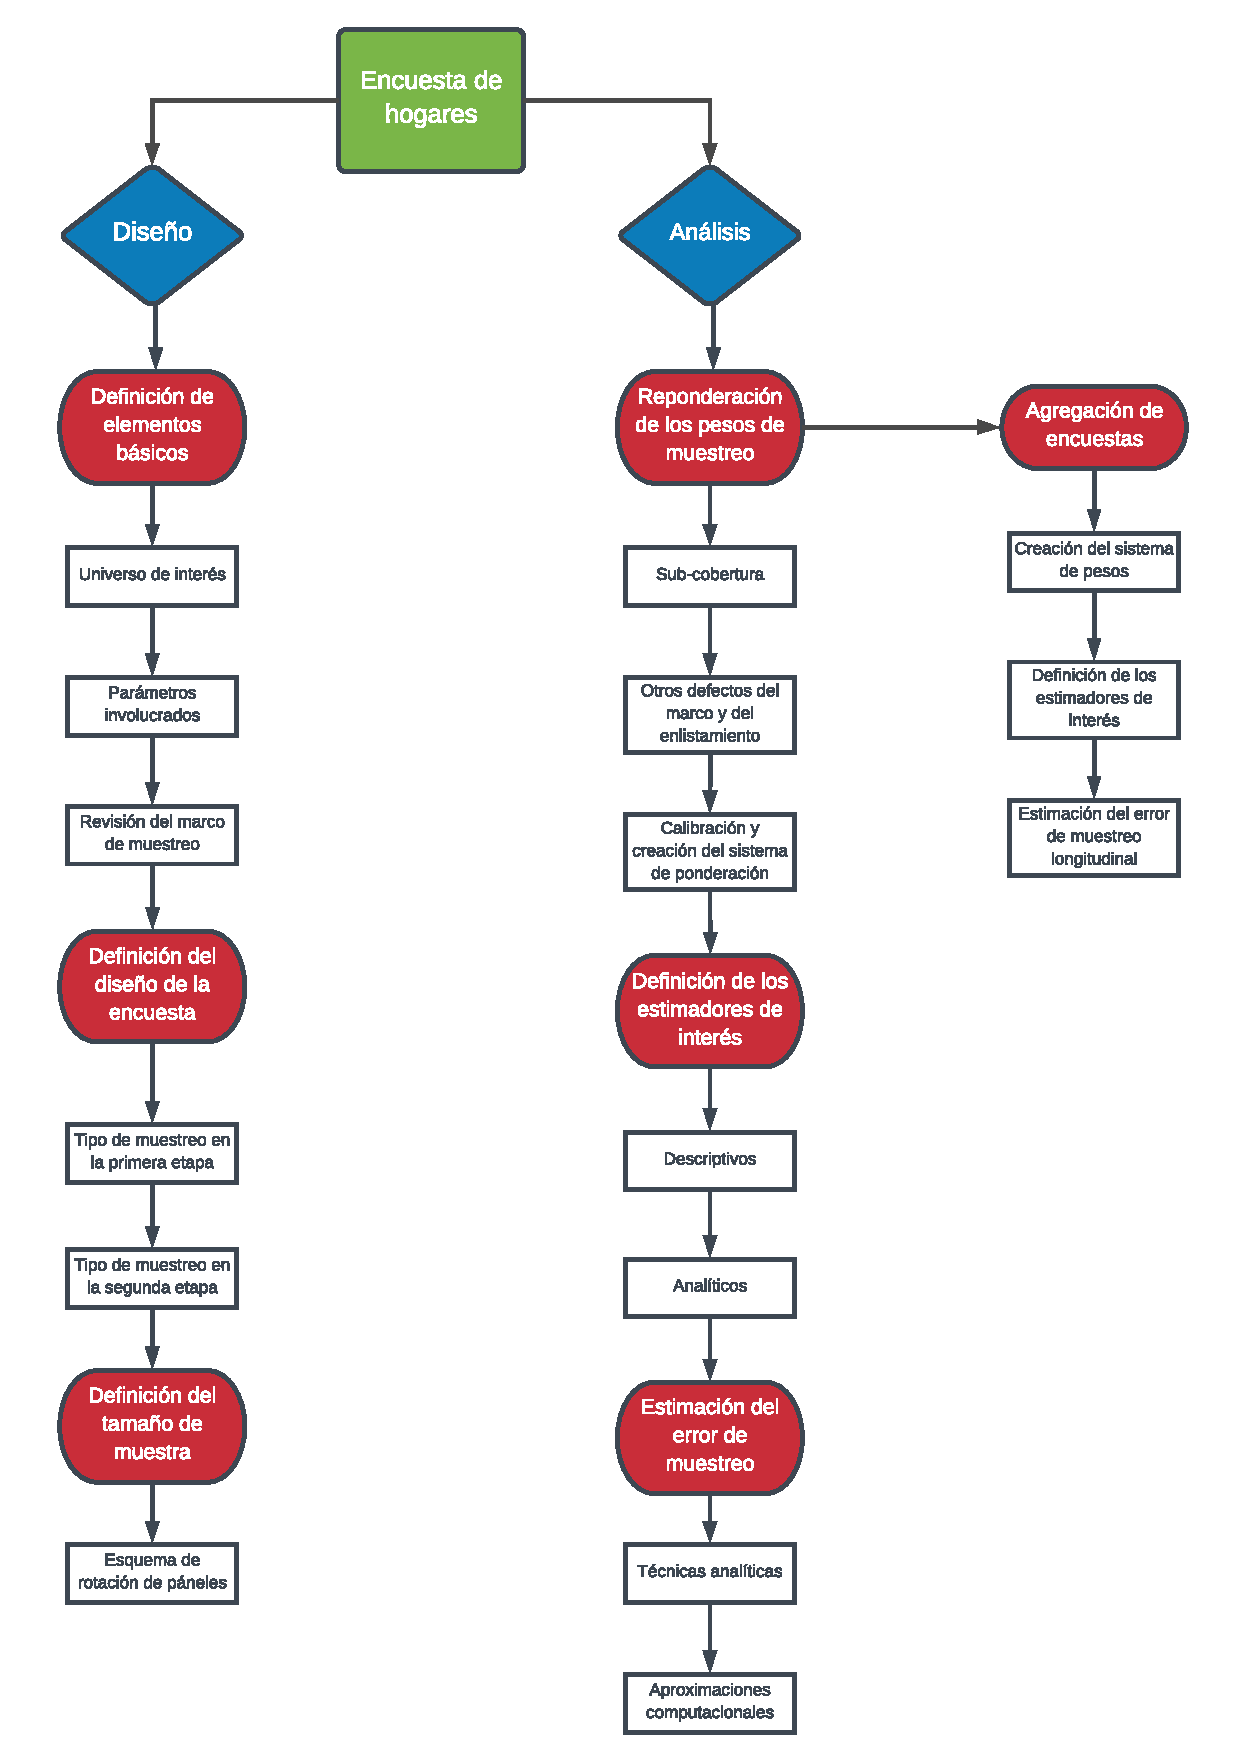
\includegraphics{Pics/1.pdf}
\caption{Esquema de procesos en el análisis y diseño de una encuesta de hogares.}
\end{figure}

En el primer capítulo se considera una breve introducción a la problemática de las encuestas de hogares. En el capítulo dos se aborda con más detalle los elementos básicos que se consideran por lo regular en los diseños de las encuestas de hogares. Un aspecto relevante de este documento es que, si bien considera que las encuestas de hogares tienen muchos elementos en común, diferencia de forma cuidadosa las particularidades de cada encuesta. Por ejemplo, en este capítulo se trata el tema del diseño de las encuestas rotativas y se profundiza en los diferentes parámetros que se pueden considerar en este tipo de operaciones; asimismo, describe las características metodológicas que se deben considerar al momento de diseñar la encuesta y revisa los conceptos esenciales que determinarán el tipo de aplicación que se debe considerar. El capítulo tres describe los principales diseños de muestreo que se utilizan en este tipo de estudios y expone de forma estándar los conceptos de estratificación y aglomeración de las poblaciones. El capítulo cuatro complementa estos conceptos con varias aplicaciones prácticas para determinar el tamaño de muestra adecuado para lograr los objetivos de la investigación. A pesar de que la literatura relacionada con la práctica del muestreo es relativamente abundante, existen pocos ejemplos prácticos que logren representar la problemática del tamaño de muestra y el lector podrá encontrar herramientas ilustrativas basadas en múltiples escenarios de la problemática social.

Pasando a la parte del análisis de las encuestas, el capítulo cinco revisa los procesos de imputación y ponderación en la encuesta. Los procesos de imputación tratan de recuperación tanta información como sea posible para que el investigador pueda contar con una base de datos rectangular y completa. Luego de esto, es necesario aplicar los factores de expansión a la información contenida en la base de datos para que se puedan realizar inferencias a nivel nacional o regional. Sin embargo, en aquellos casos en donde la imputación no resulta ser una técnica adecuada para completar la información faltante, es necesario realizar ajustes sistemáticos en los factores de expansión para que la muestra efectiva siga siendo una muestra representativa de toda la población. El capítulo seis analiza las principales metodologías de estimación, tanto de los parámetros de interés como de sus errores de muestreo. Si hay algo que distingue el análisis de las encuestas de cualquier otro tipo de estudio estadístico es que las propiedades importantes como insesgamiento, consistencia y eficiencia están basadas en el diseño de muestreo y no en supuestos metodológicos ligados a algún modelo estocástico. Es por esto que se presta especial atención a la estimación del error de muestreo, que no es otra cosa que una función de la varianza de las estimaciones, y se presentan las metodologías más comunes en términos de aproximaciones teóricas y computacionales al error de muestreo. El capítulo siete presenta de forma detallada los procesos que se surten cuando se agregan encuestas a lo largo de un periodo de tiempo. Acudiendo a la perspectiva del autor, el capítulo ocho presenta los criterios de calidad que se deberían tener en cuenta para decidir si una cifra, resultante de un proceso de estimación estadística basada en encuestas de hogares, debería ser o no publicada a la sociedad. Por úlitmo, el capítulo nueve presenta una discusión acerca del uso presente de las encuestas de hogares y los retos que depara el futuro en materia de la medición de indicadores sociales a través de las encuestas de hogares. Asimismo, en los anexos se contempla una revisión del software que se utiliza actualmente en los INE para llevar a cabo esta ardua tarea de diseñar y analizar las encuestas de hogares, una revisión rápida de algunas de las encuestas de la región, así como algunas directrices que se deberían considerar al momento de documentar los procesos asociados a las encuestas de hogares.

\hypertarget{elementos-basicos-y-planeacion}{%
\chapter{Elementos básicos y planeación}\label{elementos-basicos-y-planeacion}}

El fortalecimiento continuo de las investigaciones sociales es un objetivo que los institutos nacionales de estadística procuran sistemáticamente. En el caso de aquellas operaciones que conllevan la recolección de información primaria y que involucran la selección y medición de hogares y sus miembros, mantener una documentación adecuada que describa las razones por las cuales se ha optado por cierta metodología de recolección en particular es un requisito fundamental para cumplir este cometido. En este apartado se exploran diferentes métodos de recolección de la información y se discuten las diferentes particularidades en la planeación de una encuesta de hogares.

\hypertarget{universo-muestra-y-unidades}{%
\section{Universo, muestra y unidades}\label{universo-muestra-y-unidades}}

El término encuesta se encuentra directamente relacionado con una población finita compuesta de individuos a los cuales es necesario observar y medir. Este proceso muchas veces es realizado por medio de una entrevista. El conjunto de unidades de interés recibe el nombre de \emph{población objetivo} o \emph{universo} y sobre ellas se obtiene la información de interés para el estudio. Por ejemplo, \emph{la Encuesta Nacional de Empleo y Desempleo} de Ecuador define su población objetivo como todas las personas mayores de 10 años residentes en viviendas particulares en Ecuador.

Las \emph{unidades de análisis} corresponden a los diferentes niveles de desagregación establecidos para consolidar el diseño de la encuesta y sobre los que se presentan los resultados de interés. En México, la \emph{Encuesta Nacional de Ingresos y Gastos de los Hogares} define como unidades de análisis el ámbito al que pertenece la vivienda: urbano alto, complemento urbano y rural. Por otro lado, la \emph{Gran Encuesta Integrada de Hogres} de Colombia tiene cobertura nacional y sus unidades de análisis están definidas por 13 grandes ciudades junto con sus áreas metropolitanas.

Como se explicará más adelante, es muy difícil contar con una lista actualizada de todos los hogares del país; por lo tanto, para recolectar la información de la población objetivo, el diseño de una encuesta de hogares en América Latina plantea la necesidad de seleccionar en varias etapas ciertas \emph{unidades de muestreo} que sirven como medio para seleccionar finalmente a los hogares y personas que participarán de la muestra. Cuando se requiere seleccionar personas, se hace necesario seleccionar un subconjunto de zonas geográficas; para cada zona seleccionada, se procede a seleccionar a su vez un subconjunto de secciones cartográficas, que antecede a la selección de hogares y, finalmente, para cada hogar se seleccionan las personas; siendo estas las unidades de observación. Por ejemplo, se puede citar la experiencia de Brasil con la \emph{Pesquisa Nacional por Amostra de Domicilios} que se realiza por medio de una muestra de viviendas en tres etapas: las unidades primarias de muestreo (UPM) son los municipios, mientras que las unidades secundarias de muestreo (USM) son los sectores censales, que conforman una malla territorial conformada en el último Censo Demográfico. Por último, las unidades finales en ser seleccionadas son las viviendas.

\textcite[pág. 105]{Duncan_Kalton_1987} afirman que la composición de la población de interés en las encuestas de hogares cambia durante el tiempo, puesto que lo individuos nacen, mueren, migran, e incluso pasan a ser parte de organizaciones que hacen que pierdan su estatus de unidad de observación. Nótese que la población objetivo de la mayoría de encuestas de hogares en América Latina se refiere a la población civil excluyendo miembros de organizaciones militares, personas en cárceles, hospitales, etc. De igual forma, se debe tener en cuenta que existen nuevos hogares que pueden crearse o desintegrarse. Por ende, los equipos técnicos de los INE que están a cargo del diseño de las encuestas de hogares, que miden de forma transversal a la población de interés, deben tener en cuenta que, aunque los objetivos de la encuesta no cambian en el tiempo, sí lo hace la población objetivo y se deben plantear esquemas de seguimiento y actualización que den cuenta de esta realidad.

\hypertarget{periodicidad-en-el-tiempo}{%
\section{Periodicidad en el tiempo}\label{periodicidad-en-el-tiempo}}

Los institutos nacionales de estadística - que son los entes encargados de administrar, diseñar, analizar y difundir los resultados de las encuestas - no realizan este tipo de levantamientos de manera aislada; de hecho una característica fundamental de estas operaciones estadísticas es que se han convertido en un insumo fundamental para realizar un seguimiento periódico de muchos indicadores de interés. Por lo tanto, muchas encuestas de hogares se realizan de forma sistemática en el tiempo. Es por esto que la planeación de la encuesta debe contemplar esta periodicidad para que el levantamiento de la información primaria en campo se haga de manera más eficiente y, de la misma forma, que la estimación de estos indicadores se pueda realizar ajustándose a los recursos de la operación. Como se mencionó anteriormente, dado que la población es dinámica en el tiempo, la planeación y análisis de este tipo de encuestas es desafiante, puesto que si la composición de la población y las características de los elementos se considerara fija, una encuesta transversal (realizada una sola vez en un periodo de tiempo largo) sería suficiente para realizar estimaciones precisas que resuelvan los objetivos del estudio.

En algunas ocasiones, basta con realizar un medición simple en un punto específico del tiempo para completar los objetivos de la investigación. Este es el caso de las encuestas de ingresos y gastos cuya periodicidad es en promedio es cada 10 años y las cuales son utilizadas para, entre muchos otros propósitos, actualizar la canasta básica familiar, de la cual se derivan los insumos básicos para la medición de la pobreza \autocite{CEPAL_2018}. Para otro tipo de problemáticas, como por ejemplo el seguimiento al mercado de trabajo, es necesario recurrir a la medición periódica a través de encuestas de hogares, en donde los cambios naturales en las características de la población hacen que realizar una medición simple en un punto del tiempo sea inviable a la luz del seguimiento y monitoreo de los indicadores de interés.

Por consiguiente, al momento de realizar la planeación de una encuesta continua o periódica se debe tener en cuenta que, a pesar de que crezca la dificultad en el diseño, es posible obtener información más oportuna para la toma de decisiones y la formulación de políticas públicas. De esta manera, y teniendo en cuenta que el tiempo hace que la estructura de las poblaciones cambie, sin importar si la constituyen individuos, hogares, familias, negocios, etc., las unidades de observación deben ser consideradas como parte de la población de interés cuando nacen, inmigran o alcanzan un umbral predefinido de edad. Asimismo, las unidades salen de la población de interés cuando mueren, emigran, o se involucran en instituciones (como el servicio militar). Por ejemplo, si las unidades son los hogares, es evidente que la población no es la misma en diferentes puntos del tiempo (por ejemplo, en dos años distintos) puesto que se crean nuevas unidades cuando los jóvenes dejan a sus padres y forman nuevos hogares independientes, o cuando ocurre una separación o un divorcio; en donde un hogar se divide en dos. Además, los hogares en donde todos sus miembros han fallecido dejan de ser parte de la población objetivo. De la misma forma, dos hogares dejan de ser parte de la población objetivo cuando se unen a través de un matrimonio o algún tipo de unión civil. Teniendo en cuenta el papel dinámico de las poblaciones y los objetivos de investigación es posible plantear diferentes tipos de levantamientos; a continuación enumeramos algunas categorías de encuestas que las oficinas nacionales de estadística realizan en la región.

\hypertarget{encuestas-transversales}{%
\subsection{Encuestas transversales}\label{encuestas-transversales}}

Este tipo de encuestas son diseñadas para recolectar información únicamente en un punto específico del tiempo, o sobre un periodo de referencia, y proveen toda la información pertinente acerca de la población particular restringida a un tiempo y periodo de recolección específico. Puesto que el propósito fundamental de este tipo de encuestas no se centra en las comparaciones intertemporales, no es posible estimar cambios de ningún tipo, a no ser que se realicen indagaciones retrospectivas. El siguiente cuadro muestra un esquema de este tipo de operaciones estadísticas en donde se observa una muestra de una población específica en un periodo de tiempo específico (Tiempo 2). Dado que es una muestra transversal, no hay un patrón de repetición en los restantes periodos.

\begin{longtable}[]{@{}ccccccc@{}}
\toprule
Muestra & Tiempo 1 & Tiempo 2 & Tiempo 3 & Tiempo 4 & Tiempo 5 & Tiempo 6\tabularnewline
\midrule
\endhead
1 & & \textbf{x} & & & &\tabularnewline
2 & & \textbf{x} & & & &\tabularnewline
3 & & \textbf{x} & & & &\tabularnewline
4 & & \textbf{x} & & & &\tabularnewline
5 & & \textbf{x} & & & &\tabularnewline
6 & & \textbf{x} & & & &\tabularnewline
\bottomrule
\end{longtable}

\hypertarget{encuestas-repetidas}{%
\subsection{Encuestas repetidas}\label{encuestas-repetidas}}

Cuando existe interés en realizar un seguimiento del fenómeno en observación durante el tiempo, entonces se utilizan encuestas repetidas que recolectan información de manera periódica. Este tipo de encuestas proveen información acerca de la dinámica de la composición de la población en el tiempo. De esta forma, en cada levantamiento se observa una muestra de la población en un tiempo determinado. Por ejemplo, el siguiente cuadro muestra un acercamiento gráfico a este tipo de encuestas en donde se evidencia el carácter sistemático de estas operaciones estadísticas; además de mostrar que no es posible medir cambios individuales porque las muestras son independientes en el tiempo.

\begin{longtable}[]{@{}ccccccc@{}}
\toprule
Muestra & Tiempo 1 & Tiempo 2 & Tiempo 3 & Tiempo 4 & Tiempo 5 & Tiempo 6\tabularnewline
\midrule
\endhead
1 & \textbf{x} & & & & &\tabularnewline
2 & & \textbf{x} & & & &\tabularnewline
3 & & & \textbf{x} & & &\tabularnewline
4 & & & & \textbf{x} & &\tabularnewline
5 & & & & & \textbf{x} &\tabularnewline
6 & & & & & & \textbf{x}\tabularnewline
\bottomrule
\end{longtable}

\hypertarget{encuestas-panel}{%
\subsection{Encuestas panel}\label{encuestas-panel}}

Las encuestas en panel están diseñadas para recolectar información periódica sobre la misma muestra en diferentes puntos del tiempo. Por definición, las unidades de muestreo son las mismas en los diferentes periodos de tiempo y, de manera general, se miden las mismas variables en cada levantamiento. Por la caracterización propia de este tipo de encuestas, sí es posible medir los cambios individuales y cambios netos sobre la población de la que se seleccionó la muestra. Sin embargo, como la muestra no cambia en ningún momento del tiempo, las inferencias que se realicen estarán supeditadas a la población de la cual se seleccionó la muestra en un principio. Si la población cambia su estructura, no será posible captar este cambio puesto que las inferencias resultantes de este tipo de encuestas no son representativas de la población actual. El siguiente cuadro muestra un esquema propio de las encuestas de panel en donde los individuos que fueron seleccionados la primera vez son observados a lo largo del tiempo.

\begin{longtable}[]{@{}ccccccc@{}}
\toprule
Muestra & Tiempo 1 & Tiempo 2 & Tiempo 3 & Tiempo 4 & Tiempo 5 & Tiempo 6\tabularnewline
\midrule
\endhead
1 & \textbf{x} & \textbf{x} & \textbf{x} & \textbf{x} & \textbf{x} & \textbf{x}\tabularnewline
2 & \textbf{x} & \textbf{x} & \textbf{x} & \textbf{x} & \textbf{x} & \textbf{x}\tabularnewline
3 & \textbf{x} & \textbf{x} & \textbf{x} & \textbf{x} & \textbf{x} & \textbf{x}\tabularnewline
4 & & & & & &\tabularnewline
5 & & & & & &\tabularnewline
6 & & & & & &\tabularnewline
\bottomrule
\end{longtable}

\hypertarget{encuestas-de-panel-dividido}{%
\subsection{Encuestas de panel dividido}\label{encuestas-de-panel-dividido}}

Para hacerle frente a las dificultades propias de las encuestas de panel y poder observar tanto los cambios individuales, como los cambios en la estructura de la población, se crearon las encuestas de panel dividido. Estas operaciones estadísticas son una combinación del diseño de panel puro y del diseño repetido y su objetivo es realizar inferencias precisas acerca de los cambios de una cohorte a través del tiempo y, al mismo tiempo, del cambio en estructura de la población actual. De esta forma, se realiza el seguimiento continuo, periódico y sistemático de una muestra a través del tiempo, pero en cada levantamiento se incluyen nuevos elementos seleccionados de la población actual. Como se señalará más adelante, este tipo de encuestas cubre con eficiencia la mayoría de indicadores de interés en un estudio de investigación social. El siguiente cuadro muestra una caracterización de estos levantamientos que fijan una muestra de panel a lo largo del tiempo, a la vez que se añaden nuevas observaciones.

\begin{longtable}[]{@{}ccccccc@{}}
\toprule
Muestra & Tiempo 1 & Tiempo 2 & Tiempo 3 & Tiempo 4 & Tiempo 5 & Tiempo 6\tabularnewline
\midrule
\endhead
1 & \textbf{x} & \textbf{x} & \textbf{x} & \textbf{x} & \textbf{x} & \textbf{x}\tabularnewline
2 & \textbf{x} & & & & &\tabularnewline
3 & & \textbf{x} & & & &\tabularnewline
4 & & & \textbf{x} & & &\tabularnewline
5 & & & & \textbf{x} & &\tabularnewline
6 & & & & & \textbf{x} &\tabularnewline
7 & & & & & & \textbf{x}\tabularnewline
\bottomrule
\end{longtable}

\hypertarget{encuestas-de-panel-rotativo}{%
\subsection{Encuestas de panel rotativo}\label{encuestas-de-panel-rotativo}}

Mantener una muestra de panel es un proceso costoso desde una perspectiva económica, pero también desde el desgaste de la fuente. Es evidente que a medida que el tiempo transcurra la propensión a responder será más baja, puesto que el entrevistado se sentirá agotado al ser visitado una y otra vez. Por lo tanto, se definen las encuestas de panel rotativo para poder realizar inferencias parciales - restringidas a periodos de tiempo específicos - del cambio individual y a la vez captar el cambio estructural de la población. Estas encuestas incorporan nuevos elementos de la población y a la vez mantienen elementos comunes con mediciones anteriores. Obviando las dificultades que acarrea la ausencia de respuesta, las encuestas panel definen un traslape completo entre las muestras de dos puntos cualesquiera en el tiempo; sin embargo, en las encuestas rotativas existe un traslape parcial, por lo que se reduce el efecto del desgaste del panel (sobre la población inicial) y el efecto de la pérdida de muestra. Además, la inclusión de nuevos elementos en la muestra provee información pertinente del cambio en la composición estructural de la población. El siguiente cuadro ejemplifica el diseño de las encuestas rotativas.

\begin{longtable}[]{@{}ccccccc@{}}
\toprule
Muestra & Tiempo 1 & Tiempo 2 & Tiempo 3 & Tiempo 4 & Tiempo 5 & Tiempo 6\tabularnewline
\midrule
\endhead
1 & \textbf{x} & & & & &\tabularnewline
2 & \textbf{x} & \textbf{x} & & & &\tabularnewline
3 & \textbf{x} & \textbf{x} & \textbf{x} & & &\tabularnewline
4 & & \textbf{x} & \textbf{x} & \textbf{x} & &\tabularnewline
5 & & & \textbf{x} & \textbf{x} & \textbf{x} &\tabularnewline
6 & & & & \textbf{x} & \textbf{x} & \textbf{x}\tabularnewline
8 & & & & & \textbf{x} & \textbf{x}\tabularnewline
9 & & & & & & \textbf{x}\tabularnewline
\bottomrule
\end{longtable}

\hypertarget{rotacion-de-paneles}{%
\section{Rotación de páneles}\label{rotacion-de-paneles}}

Algunas encuestas de hogares en América Latina permiten que un hogar sea visitado en más de una ocasión con el fin de tener estimaciones precisas acerca de los cambios de estado que el hogar o las personas que lo habitan puedan sufrir. Por ejemplo, un hogar que en un periodo estuvo en condición de pobreza extrema, puede estar en otro periodo en condición de pobreza o inclusive puede pasar a estar fuera de la pobreza; en las encuestas de fuerza laboral, una persona puede pasar de estar empleada en un periodo a desempleada en otro periodo. Estos cambios y la dinámica propia que conllevan son de interés para los investigadores y deben ser contemplados desde una perspectiva más amplia en cuanto a su diseño. Nótese que este tipo de variaciones sobre los individuos necesariamente tiene que ser captada a través de un componente de panel, por lo que las encuestas transversales o repetidas no serían viables para realizar estas estimaciones.

En América Latina hay una gran variedad de encuestas de hogares que utilizan diseños rotativos (ver anexo). Por ejemplo, la \emph{Encuesta Permanente de Hogares} en Argentina renueva periódicamente el conjunto de hogares que serán entrevistados mediante un esquema\footnote{Un esquema de rotación \(x(y)z\), se define como aquel en donde la vivienda entra al panel por \(x\) meses, se excluye por los siguientes \(y\) meses y este patrón se repite \(z\) veces en el tiempo.} de rotación \(2(2)2\) que selecciona a las viviendas para ser entrevistadas en dos periodos consecutivos, luego los siguientes dos periodos esas viviendas salen de la selección, para finalmente volver a ser encuestadas en los siguiente dos periodos. De esta forma, un hogar es seguido a lo largo de 18 meses y esto permite cumplir con los objetivos de la encuesta. Este esquema induce algunas propiedades interesantes, que pueden ser ejemplificadas usando el siguiente cuadro definido para los cuatro trimestres de los años 2016, 2017, 2018 en cuatro grupos de muestra A, B, C y D.

\begin{itemize}
\tightlist
\item
  Entre el primer y el segundo periodo de medición hay un traslape del 50\% de hogares. En particular, nótese que entre 2016-T1 y 2016-T2, la muestra se conserva en un 50\%, puesto que \(a1\) y \(d1\) se repiten. Esto mismo sucede en cada trimestre del esquema rotacional.
\item
  En el tercer periodo no habrá traslape con el primer periodo. Nótese que 2016-T1 y 2016-T3 no existe ningún elemento en común. De la misma manera, entre 2016-T2 y 2016-T4, no existe ningún elemento en común. Este mismo patrón se encuentra a lo largo del esquema rotacional.
\item
  En el cuarto periodo se tendrá un 25\% de traslape con el primer periodo. Nótese, por ejemplo, que entre 2017-T1 y 2017-T4, \(d3\) se repite; de la misma manera, entre 2017-T4 y 2018-T3, \(d4\) se repite.
\item
  Finalmente en el quinto periodo se volverá a tener un 50\% de traslape con respecto al primer periodo. Por ejemplo, 2016-T1 y 2017-T1 comparten el 50\% de la muestra \(a1\) y \(b1\); asimismo, 2017-T1 y 2018-T1 comparten el 50\% de la muestra \(c3\) y \(b3\).
\end{itemize}

\begin{longtable}[]{@{}cccccc@{}}
\caption{\emph{Rotación de páneles en un diseño 2(2)2.}}\tabularnewline
\toprule
Año & Trimestre & A & B & C & D\tabularnewline
\midrule
\endfirsthead
\toprule
Año & Trimestre & A & B & C & D\tabularnewline
\midrule
\endhead
2016 & T1 & \emph{a1} & \emph{b1} & \emph{c1} & \emph{d1}\tabularnewline
& T2 & \emph{a1} & \emph{b2} & \emph{c2} & \emph{d1}\tabularnewline
& T3 & \emph{a2} & \emph{b2} & \emph{c2} & \emph{d2}\tabularnewline
& T4 & \emph{a2} & \emph{b1} & \emph{c3} & \emph{d2}\tabularnewline
2017 & T1 & \emph{a1} & \emph{b1} & \emph{c3} & \emph{d3}\tabularnewline
& T2 & \emph{a1} & \emph{b2} & \emph{c4} & \emph{d3}\tabularnewline
& T3 & \emph{a2} & \emph{b2} & \emph{c4} & \emph{d4}\tabularnewline
& T4 & \emph{a2} & \emph{b3} & \emph{c3} & \emph{d4}\tabularnewline
2018 & T1 & \emph{a3} & \emph{b3} & \emph{c3} & \emph{d3}\tabularnewline
& T2 & \emph{a3} & \emph{b4} & \emph{c4} & \emph{d3}\tabularnewline
& T3 & \emph{a4} & \emph{b4} & \emph{c4} & \emph{d4}\tabularnewline
& T4 & \emph{a4} & \emph{b3} & \emph{c5} & \emph{d4}\tabularnewline
\bottomrule
\end{longtable}

Otro ejemplo de una encuesta que utilizada rotación de paneles es la \emph{Encuesta Continua de Empleo} que, aplicada por el Instituto Nacional de Estadística de Bolivia, hace uso de una metodología mixta que permite el seguimiento continuo y transversal a la tasa de desempleo y a la tasa de subocupación, así como el seguimiento a los cambios que se presentan entre los periodos de interés (trimestres y semestres), a través del análisis longitudinal de los datos en el sector urbano (pues el diseño no es rotativo en el sector rural, debido a la baja incidencia de desempleo en esta zona). En este esquema rotacional 4(0)1 una vivienda es entrevistada durante cuatro trimestres consecutivos, y luego sale del panel definitivamente. Un ejemplo de este tipo de esquemas se presenta en el siguiente cuadro.
- Nótese que entre el primer y el segundo periodo de medición hay un traslape del 75\% de hogares. En particular, entre 2016-T1 y 2016-T2, la muestra se conserva en tres cuartas partes puesto que \(a1\), \(c1\) y \(d1\) se repiten. Esto mismo sucede en cada trimestre del esquema rotacional.
- Por otro lado, entre el primer y el tercer periodo habrá un traslape del 50\%. Nótese que entre 2016-T1 y 2016-T3, la mitad de la muestra se conserva puesto que \(a1\) y \(c1\) se repiten. Este mismo patrón se encuentra a lo largo del esquema rotacional.
- Entre el primer y el cuarto periodo se tendrá un 25\% de traslape. Nótese, por ejemplo, que entre 2017-T1 y 2017-T4, \(a2\) se repite; de la misma manera, entre 2017-T4 y 2018-T3, \(d3\) se repite.
- Finalmente entre el primer y quinto periodo no se tiene ningún tipo de traslape.

\begin{longtable}[]{@{}llllll@{}}
\caption{\emph{Rotación de páneles en un diseño 4(0)1.}}\tabularnewline
\toprule
Año & Trimestre & A & B & C & D\tabularnewline
\midrule
\endfirsthead
\toprule
Año & Trimestre & A & B & C & D\tabularnewline
\midrule
\endhead
2016 & T1 & \emph{a1} & \emph{b1} & \emph{c1} & \emph{d1}\tabularnewline
& T2 & \emph{a1} & \emph{b2} & \emph{c1} & \emph{d1}\tabularnewline
& T3 & \emph{a1} & \emph{b2} & \emph{c2} & \emph{d1}\tabularnewline
& T4 & \emph{a1} & \emph{b2} & \emph{c2} & \emph{d2}\tabularnewline
2017 & T1 & \emph{a2} & \emph{b2} & \emph{c2} & \emph{d2}\tabularnewline
& T2 & \emph{a2} & \emph{b3} & \emph{c2} & \emph{d2}\tabularnewline
& T3 & \emph{a2} & \emph{b3} & \emph{c3} & \emph{d2}\tabularnewline
& T4 & \emph{a2} & \emph{b3} & \emph{c3} & \emph{d3}\tabularnewline
2018 & T1 & \emph{a3} & \emph{b3} & \emph{c3} & \emph{d3}\tabularnewline
& T2 & \emph{a3} & \emph{b4} & \emph{c3} & \emph{d3}\tabularnewline
& T3 & \emph{a3} & \emph{b4} & \emph{c4} & \emph{d3}\tabularnewline
& T4 & \emph{a3} & \emph{b4} & \emph{c4} & \emph{d4}\tabularnewline
\bottomrule
\end{longtable}

Los diseños de las encuestas de hogares deben tener en cuenta la rotación de los paneles y el número de veces que es visitado un hogar. Esta caracterización depende directamente de los indicadores a los cuales la encuesta debe responder. Por ejemplo, el diseño de rotación debe ser diferente si el interés se centra en indicadores de cambio trimestral, a si se requieren indicadores de cambio anual. Por ejemplo, si el objetivo está en comparar las estimaciones de la tasa de desocupación el mismo mes entre diferentes años, el diseño 4(0)1 no es conveniente puesto que el traslape anual es nulo. En cualquier caso debe existir un esquema longitudinal, pero la diferencia principal radica en el tiempo en el que un hogar pertenecerá al panel. Por supuesto, hay que tener en cuenta que la tasa de ausencia de respuesta y pérdida de muestra por desgaste crecerá en la medida en que se le pida a un hogar una participación más duradera en el tiempo.

La definición de los indicadores de interés debe primar sobre el diseño de las encuestas de hogares. Por ejemplo, si el objetivo de la encuesta se centra en la estimación del cambio del indicador en dos periodos de tiempo, entonces el cálculo de la precisión de las estimaciones debe tener en cuenta que las muestras no son independientes y por lo tanto se debe calcular la varianza de la primera ronda, la varianza de la segunda ronda y la correlación entre las dos rondas de interés. Estos tres componentes deben intervenir en el cálculo de los coeficientes de variación, así como en la determinación del tamaño de muestra en cada ronda. En efecto, como lo afirma \textcite[pág. 236]{McLaren_Steel_2001}, para la estimación de tendencias, definidas a partir de series de tiempo macroeconómicas de los parámetros de interés en los estudios de fuerza laboral, el mejor patrón encontrado es el 1(2)m, en donde la vivienda entra en un primer mes en el panel, se excluye por los siguientes dos meses y este patrón se repite \(m\) veces consecutivas. A partir de allí la vivienda ya no vuelve a ser incluida en el estudio. En resumen, por la naturaleza de las encuestas de hogares en la región, al momento de pensar en incluir o cambiar la estructura rotacional en el sistema de encuestas de hogares, se debería considerar en primer lugar el esquema de repartición de paneles mensual. Una mirada más profunda de este tipo de análisis longitudinales se encuestar presente en el último capítulo de este documento.

\hypertarget{parametros-de-interes}{%
\section{Parámetros de interés}\label{parametros-de-interes}}

Las encuestas son usadas para producir estimaciones de parámetros que describen la situación de una población, respondiendo a los objetivos de la investigación. Por lo general, y como se describirá más adelante, el conocimiento de la población a cualquier nivel está reflejado en forma de totales, o de funciones de totales. Es por esta razón que este documento se enfoca y profundiza en las características inferenciales de los totales, puesto que la generalización a otros parámetros es inmediata. De esta manera, un \textbf{total poblacional} se define como la suma de las observaciones de una variable de interés, notada como \(y\), en la población. Se calcula mediante la siguiente ecuación:

\[t_y = \sum_U y_k\]
En donde \(U\) hace referencia al universo de estudio e \(y_k\) hace referencia a la variable de interés en el \(k\)-ésimo individuo. Por ejemplo, en una investigación social se puede realizar una encuesta para estimar el total de gasto de los hogares de un país en productos específicos de comida y bebidas no alcohólicas. En este ejemplo, la población \(U\) corresponde a los hogares, mientras que la variable \(y\) corresponde al gasto en comida y bebidas no alcohólicas, que es observada en el \(k\)-ésimo hogar, y notada como \(y_k\).

Un caso particular de este parámetro es el \textbf{tamaño poblacional} que designa la cantidad de unidades que conforman una población y se denota como \(N\). Por lo general, este parámetro es regularmente conocido, o al menos se tiene una aproximación de esta cantidad. En una encuesta de hogares, este parámetro podría denotar el número de hogares en el país - el cual no es conocido literalmente, aunque sí se conocen aproximaciones (o proyecciones) a esta cantidad con base en los resultados de los censos de población y vivienda - o el número de habitantes del país - el cual tampoco es conocido exactamente, aunque sí se cuente con proyecciones poblacionales.

Tal vez el parámetro más relevante en la investigación social lo constituye el \textbf{promedio poblacional} que describe la cantidad que debería ser asignada a cada individuo de la población si hubiese una asignación equitativa de la variable de interés. De esta forma, el promedio se define como la suma de las observaciones de la variable en la población dividida por el tamaño poblacional \(N\) y se calcula mediante la siguiente expresión:

\[\bar{y}_U = \frac{t_y}{N}\]

Por ejemplo, en una encuesta de hogares es posible estimar el ingreso medio de la población, definido como el total de los ingresos de todos los hogares del país dividido entre el número de habitantes del país. En este caso la variable de interés \(y\) es el ingreso per cápita. De la misma forma, también se podría estimar el gasto promedio de los hogares en educación; en donde la variable de interés \(y\) es el gasto de todos lo miembros del hogar en este concepto (sin importar la edad ni el nivel propedéutico) y \(N\) sería el número de hogares del país.

La incidencia de los fenómenos sociales sobre los hogares o personas puede ser medida a través de la \textbf{proporción poblacional}, que es un parámetro definido como un promedio sobre una variable dicotómica \(z_k\) que toma el valor de 1 si el \(k\)-ésimo individuo tiene el atributo de interés y de 0 en otro caso. Se calcula mediante la siguiente ecuación:

\[P_U=\frac{\sum_U z_k}{N}\]

Por ejemplo, la proporción de personas en condición de pobreza es una proporción sobre toda la población, en donde la variable de interés \(z\) indica si el ingreso per cápita de un individuo es menor que la línea de pobreza; \textcite{CEPAL_2018} presenta los pormenores metodológicos del cálculo de la pobreza en los países de América Latina y el Caribe. Por otro lado, la \textbf{razón poblacional} se calcula como el cociente entre dos totales, el primer total asociado a una variable de interés \(y\), el segundo total asociado a una variable de interés \(z\). Este parámetro se calcula mediante la siguiente expresión:

\[R_U=\frac{t_y}{t_z}\]

en donde \(t_y\) es el total poblacional asociado a la variable \(y\), \(t_z\) es el total asociado a la variable \(z\). Por ejemplo, en la medición del mercado de trabajo, la tasa de desocupación es una razón entre el total de personas desocupadas y el total de personas activas. Nótese que para clasificar a una persona como desocupada, ocupada, activa o inactiva, es necesario realizar una indagación en la encuesta a cada uno de los miembros del hogar; por lo tanto ambas cantidades, numerador y denominador, corresponden a cantidades desconocidas de antemano. Es más, la condición de ocupación de las personas puede variar entre los periodos de observación. Con respecto a indicadores de pobreza, otro tipo de parámetros pueden expresarse como razones poblacionales; es el caso de la brecha de pobreza y de la incidencia de la pobreza expresada en términos de un umbral de poder adquisitivo \autocite{Foster_Greer_Thorbecke_1984}. Este tipo de indicadores complejos se pueden expresar mediante la siguiente relación

\[
F_{\alpha} = \frac{1}{N} \sum_U \left(\frac{u-y_k}{u}\right)^{\alpha}
\]

En donde \(y_k\) determina el ingreso del individuo \(k\), \(u\) se refiere al umbral que establece la línea de pobreza y \(\alpha\) pertenece al intervalo \((0, 1)\). Por ejemplo, en el caso en el que \(\alpha = 0\), este indicador calcula la tasa de pobreza, que es la incidencia de este fenómeno en la población; si \(\alpha = 1\), este indicador calcula la brecha de la pobreza, que es la cantidad de dinero que se necesitaría en promedio para que un país no tuviera personas en situación de pobreza. En este punto vale la pena resaltar que en la definición de los parámetros básicos que se quieren estimar en una encuesta, el papel de los totales poblacionales es absolutamente relevante. De igual manera, existen otros parámetros que pueden ser considerados complejos - no por su forma funcional, sino por los procesos complejos que hay detrás del levantamiento de la información primaria - pero que al igual que los mencionados anteriormente resultan ser también una función de totales poblacionales. Por ejemplo, considere el \textbf{cambio neto} de los totales de la variable de interés \(y\) en dos periodos de tiempo (\(t_1\) y \(t_2\)) dado por la siguiente expresión:

\[
\Delta_y = t_{y}^2 - t_{y}^1
\]

Este tipo de parámetros son muy comunes en las encuestas que se realizan para conocer la estructura y los cambios del mercado de trabajo. Por ejemplo, la siguiente tabla muestra la composición del mercado de trabajo en una población observada en dos periodos de interés (las cifras están en millones). De esta forma, los totales marginales de la tabla corresponden a los \textbf{cambios netos} que permiten una comparación simple con el periodo anterior. Específicamente, es posible observar que hay 313 mil empleados menos, 80 mil desempleados menos y 393 mil inactivos más en el segundo periodo, en comparación al primero.

\begin{longtable}[]{@{}lllll@{}}
\caption{\emph{Composición del mercado de trabajo en dos periodos de tiempo}}\tabularnewline
\toprule
Condición & Ocupado & Desocupado & Inactivo & Total\tabularnewline
\midrule
\endfirsthead
\toprule
Condición & Ocupado & Desocupado & Inactivo & Total\tabularnewline
\midrule
\endhead
Ocupado & 9222 & 128 & 662 & 10012\tabularnewline
Desocupado & 221 & 322 & 151 & 694\tabularnewline
Inactivo & 256 & 164 & 5941 & 6361\tabularnewline
Total & 9699 & 614 & 6754 & 17067\tabularnewline
\bottomrule
\end{longtable}

Una comparación más profunda está dada en términos de los \textbf{cambios brutos}, que corresponden a las entradas de la tabla cruzada. De esta manera, los cambios en la fuerza de trabajo de un periodo a otro, se explican porque el 92.1\%=(9222/10012)\% de los empleados conservó su empleo; el 31.8\% de los desempleados y el 4.0\% de los inactivos consiguió un nuevo empleo; el 6.6\% de los empleados es ahora inactivo en la fuerza laboral y el 1.3\% de los empleados perdió su empleo. Así mismo, el 46.4\% de los desempleados conservó su clasificación; el 1.3\% de los empleados perdió su empleo y el 2.6\% de los inactivos entró a la fuerza laboral como desempleado; el 31.8\% de los desempleados es ahora empleado y el 21.8\% de los desempleados es ahora inactivo.

\hypertarget{ejemplos-de-indicadores-de-interes-y-su-relacion-con-los-tipos-de-encuestas}{%
\subsection{Ejemplos de indicadores de interés y su relación con los tipos de encuestas}\label{ejemplos-de-indicadores-de-interes-y-su-relacion-con-los-tipos-de-encuestas}}

En esta sección se relacionan algunos de los parámetros anteriormente mencionados con los tipos más comunes de encuestas. Estos ejemplos nos presentan algunas indicaciones del tipo de encuestas que se encuentran en América Latina y examinan el raciocinio detrás de estos levantamientos. Tomando en consideración las características generales de las encuesta de hogares, \textcite{Duncan_Kalton_1987} mencionan las siguientes situaciones, ejemplificadas a continuación.

\begin{itemize}
\item
  \textbf{Estimación de parámetros poblacionales en un punto del tiempo}. Por ejemplo, suponga que se quiere estimar el \emph{ingreso per cápita promedio por área (rural - urbano) en las regiones de un país}. En este tipo de estudios, la encuestas aptas serían las transversales, las repetidas, las de panel rotativo y las de panel dividido. Nótese que las encuestas de panel puro no son aptas para captar este parámetro puesto que la muestra no es representativa de la población en el momento actual, sino que, por el contrario, es representativa de la población en el momento en la cual se extrajo la muestra.
\item
  \textbf{Estimación de cambios netos}. Si se quisiera estimar la \emph{diferencia en el número de ocupados de la fuerza de trabajo entre el segundo trimestre de 2018 y el primer trimestre de 2018 en un país}, entonces las encuestas aptas serían las repetidas, las de panel rotativo y las de panel dividido. Una encuesta transversal no sería apta para lograr esta estimación, puesto que su frecuencia de realización no es trimestral. De la misma forma que en el parámetro anterior, las encuestas de panel puro no son aptas para captar este parámetro puesto que la muestra no es representativa de la población en el momento actual.
\item
  \textbf{Estimación de cambios brutos y componentes individuales}. Para estimar el \emph{porcentaje de personas ocupadas en el segundo trimestre de 2018 que estuvieron desocupadas en el primer trimestre de 2018 en un país} es necesario que la encuesta tenga algún patrón de selección de los mismos individuos en los dos periodos. De esta forma, las únicas encuestas aptas para estimar este cambio bruto son las de panel, panel rotativo y panel dividido. Las encuestas transversales o repetidas no podrían arrojar este tipo de estimativas puesto que su diseño no considera a los mismos individuos en la muestra en dos periodos de tiempo.
\item
  \textbf{Estimación de la incidencia de eventos en un periodo de tiempo}. Suponga que se quiere estimar la \emph{proporción de mujeres que fueron víctimas de un evento de violencia en los úlitmos seis meses en un país}. En este caso todas las encuestas resultarían aptas mediante ligeras modificaciones en el diseño. Por ejemplo, la encuesta transversal debería preguntar de forma retrospectiva; las encuestas repetidas podrían ser agregadas en los últimos seis meses, las encuestas de tipo panel rotativo y divididas deberían preguntar en cada medición de los últimos seis meses por este evento.
\item
  \textbf{Estimación de la incidencia de eventos raros en el tiempo}. Por ejemplo, si se quisiera estimar la \emph{proporción de personas con una enfermedad rara}, es posible que las encuestas transversales y de tipo panel no sean aptas. En el primer caso, dado que el evento es raro por definición, los requerimientos de tamaño de muestra en una encuesta transversal sobrepasarían el presupuesto y los costos de la encuesta; en el segundo caso, además de las consideraciones anteriormente planteadas del tamaño de muestra, por la misma definición de evento raro, tampoco sería plausible que en el panel se presentaran estos eventos en los individuos a través del tiempo. Por otro lado, al agregar las encuestas repetidas, las de panel rotativas y la parte nueva del panel dividido, sería posible llegar al tamaño de muestra adecuado para poder captar esta incidencia de forma precisa y eficiente.
\end{itemize}

Estos últimos ejemplos muestran la importancia de contar con procedimientos adecuados de acumulación de datos y encuestas a lo largo de un periodo de interés, por ejemplo de forma anual o semestral. La acumulación de datos genera todo tipo de parámetros en una ventana más amplia del tiempo. Es posible acumular datos eficientemente por medio de la agregación de encuestas repetidas. De esta forma se definiría una agregación de datos vertical que añade filas, puesto que en cada levantamiento aparecen nuevos individuos, dado que el diseño de las encuestas repetidas selecciona diferentes individuos en cada punto del tiempo. Este es el caso de la \emph{Gran Encuesta Integrada de Hogares de Colombia} que está diseñada para tener representatividad a niveles de desagregación mayores, juntando los individuos observados en los doce levantamientos continuos en un año. Por otro lado, las encuestas de panel permiten un tipo diferente de agregación, no basado en individuos, sino en variables en el tiempo. A diferencia de las encuestas repetidas, las encuestas de panel, panel rotativo o panel dividido permiten observar a los individuos en diferentes periodos de tiempo y la agregación puede hacerse de forma horizontal, manteniendo a los individuos en las filas y añadiendo columnas cada vez que se observe una nueva medición en un periodo de tiempo diferente.

\hypertarget{seleccion-de-la-muestra}{%
\chapter{Selección de la muestra}\label{seleccion-de-la-muestra}}

Todas las encuestas de hogares en la región comparten el mismo principio inferencial: la selección de una pequeña muestra que puede representar la población de todo un país. Por supuesto, ante este objetivo tan ambicioso, es necesario contar con procedimientos robustos, probados y capaces de pasar los filtros más críticos y agudos. Tal vez en este momento de la historia, la práctica de estos procedimientos ya no genere ningún tipo de asombro, pero el lector podría animarse a contemplar todas los posibles escenarios que una sociedad enfrentaría ante la ausencia de las encuestas de hogares y sus repercusiones en materia del desarrollo social. Es innegable la potencia y el poder que hay detrás de estas operaciones estadísticas que están sustentadas en el muestreo probabilístico que induce una inferencia que procede de lo particular a lo general, puesto que al seleccionar una muestra, esta sirve como base para obtener conclusiones acerca de la población. Al final la muestra será un vehículo adecuado para representar las características más importantes de la población en estudio, en la forma en que justamente las variables se incorporan en el formulario de la encuesta. \textcite{Gutierrez_2016} afirma que el muestreo es un procedimiento que responde a la necesidad de información estadística precisa sobre la población y los conjuntos de elementos que la conforman; el muestreo probabilístico trata con investigaciones parciales sobre la población que apuntan a inferir a la población completa y en general está basado en los siguientes principios:

\begin{itemize}
\tightlist
\item
  \emph{Aleatorización}: las unidades incluidas en la muestra son seleccionadas mediante un proceso probabilístico. De esta forma, además de eliminar los posibles sesgos de selección, la muestra resultante será válida para cualquier proceso de inferencia, puesto que se basa en el conjunto de todas las muestras que se pueden obtener con el esquema de muestreo definido.
\item
  \emph{Inclusión}: todas las unidades de la población tienen una probabilidad no nula de ser incluidas en la muestra. Lo anterior quiere decir que el procedimiento de selección le da chance de ser seleccionado a todas las unidades que componen la población. De esta manera, la muestra final puede estar compuesta por cualquier combinación plausible de hogares o individuos.
\end{itemize}

Por supuesto, para que los anteriores principios se cumplan a cabalidad, es necesario contar con un instrumento que permita seleccionar a los hogares del país de forma exhaustiva y completa; esto quiere decir que el instrumento debería contener todos y cada uno de los hogares de la población. Dado que no existe una lista que permita identificar y ubicar cada uno de los hogares de la población, entonces se deben contemplar otras posibilidades que permitan lograr el objetivo. Debido al principio natural de la aglomeración social de las poblaciones humanas, es posible lograr este cometido de manera indirecta a través de la definición de marcos de muestreo de áreas.

\hypertarget{marcos-de-muestreo-estratificacion-y-aglomeracion}{%
\section{Marcos de muestreo: estratificación y aglomeración}\label{marcos-de-muestreo-estratificacion-y-aglomeracion}}

Para realizar el proceso de selección sistemática de los hogares es necesario contar con un marco de muestreo que sirva de vínculo entre los hogares y las unidades de muestreo y que permita tener acceso a la población de interés. Como regla general, el marco de muestreo debe permitir \emph{identificar} y \emph{ubicar} a todos los hogares que conforman la población objetivo. Como lo afirma \textcite{Gutierrez_2016}, el marco de muestreo más utilizado en este tipo de encuestas es de áreas geográficas que vinculan directamente a los hogares o personas. Por esta razón, los diseños de muestreo de estas encuestas se apoyan en la aglomeración natural de los hogares en segmentos cartográficos, que a su vez están contenidos en agrupaciones mayores. ¿Cómo se aglomeran las personas y cómo podemos realizar un diseño de muestreo con base en esta forma de aglomeración? Pues bien, las personas se aglomeran en hogares, los cuales a su vez se aglomeran en comunidades más grandes: barrios, comunas, segmentos. Estas comunidades forman ciudades y la reunión de estas divisiones es el país. Por lo tanto, a pesar de que ningún país tiene a disposición una lista actualizada de todos los hogares junto con su ubicación e identificación, sí existe en todos los países una lista actualizada de los segmentos cartográficos presentes en las zonas urbanas y rurales. De esta forma, si se selecciona de forma probabilística una muestra de sectores y dentro de cada sector se selecciona de forma probabilística una muestra de hogares, entonces de forma indirecta estaremos seleccionando una muestra de hogares que puede representar la realidad de todo un país.

Como se mencionó anteriormente, una característica esencial de los diseños de las encuestas de hogares es que la selección de las unidades finales de muestreo debe surtir varias etapas, de acuerdo a las agrupaciones definidas en los marcos de muestreo, que usualmente son marcos de área obtenidos de la división geográfica del país, región o municipio en áreas menores mutuamente excluyentes. Los institutos de estadística en América Latina hacen grandes esfuerzos para mantener actualizados sus marcos de muestreo. Por ejemplo, la \emph{Encuesta Nacional de Hogares} de Costa Rica utiliza un marco muestral construido a partir de los censos nacionales de población y vivienda de 2011 y corresponde a un marco de áreas en donde sus unidades son superficies geográficas asociadas con las viviendas. Este marco en particular permite la definición de UPM con 150 viviendas en las zonas urbanas y 100 viviendas en las zonas rurales. En general, el marco está conformado por 10461 UPM (64.5\% urbanas y 35.5\% rurales). \textcite{Gambino_Silva_2009} mencionan que, en la práctica, la consecución de los marcos de lista de lo hogares en la última etapa del muestreo puede tornarse difícil puesto que dentro del conglomerado no es obvio observar de manera exhaustiva los hogares, especialmente cuando la frontera del conglomerado es una línea imaginaria. Por ejemplo en lo urbano, la distinción entre dos conglomerados está demarcada claramente por las calles que conforman la ciudad; sin embargo, en la ruralidad, difícilmente existen caminos que puedan servir para delimitar los conglomerados. De la misma manera, esta delimitación se torna compleja cuando han ocurrido cambios en la infraestructura del área y aparecen nuevas construcciones.

Observe que en general, ante el estudio de un fenómeno social, las desagregaciones geográficas más amplias constituyen un interés natural para los usuarios de las encuestas; es así como los investigadores que planean las encuestas quisieran poder desagregar la información por las regiones geográficas más grandes, que a su vez tienen cierta independencia política y administra. Las estadísticas nacionales que se publican a partir de las encuestas de hogares, cobran mayor relevancia a nivel de regiones, estados o departamentos. Este tipo de desagregaciones geográficas se conocen con el nombre de estratos. Inclusive los diseños de las encuestas de hogares han ido evolucionando para permitir que este tipo de agregaciones tenga representatividad en la encuesta. Aunado a lo anterior, si la característica de interés con la cual se planea la encuesta hace que la distribución de la población sea altamente sesgada, como en el caso de los ingresos o gastos, es recomendable crear un estrato de inclusión forzosa con las unidades más importantes en la población. Esta práctica asegura que el error de muestreo sea más bajo. Algunos países hacen uso de la información censal para definir una estratificación socio económica sobre los segmentos cartográficos del marco de muestreo utilizando para tal fin algunas preguntas del censo de población más reciente. Esta práctica representa una ventaja metodológica porque, en la mayoría de encuestas, los parámetros de interés tienen un comportamiento estructural diferente en cada uno de los subgrupos poblacionales creados, tendiendo a tener una mayor precisión en la estimación de los parámetros de interés. Por ejemplo, utilizando las preguntas del censo, es posible crear un índice de condiciones de vivienda y con este definir algunos grupos de viviendas mutuamente excluyentes que contengan viviendas parecidas dentro de ellos, pero que entre ellos sean muy disimiles. De esta forma, es posible estratificar los sectores cartográficos de todo un país y generar estimaciones más precisas de los indicadores sociales (como pobreza, ingreso medio, etc.) si el diseño de muestreo contempla este tipo de estratificación.

Para el caso de la \emph{Gran Encuesta Integrada de Hogares} en Colombia, los criterios de estratificación forman dos grupos: el primero correspondiente a las 24 capitales junto con sus correspondientes áreas metropolitanas y el segundo correspondiente al resto de cabeceras municipales, centros poblados y la ruralidad dispersa. Además, la encuesta también contempla criterios de estratificacion económica a nivel municipal como nivel de urbanización y estructura de la población, basada en la proporción de habitantes con necesidades básicas insatisfechas. De la misma manera, el diseño de la muestra maestra del Instituto Nacional de Estadística y Geografía de México contempla este tipo de estratificación basada en los indicadores generados con la información del Censo de Población y Vivienda 2010. Previo al proceso de estratificación sociodemográfica, fue necesario construir y seleccionar una serie de variables que lograran, en conjunto, separar el universo de UPM en agrupaciones que mejoraran las principales estimaciones de las diferentes encuestas usuarias del Marco de Muestreo \autocite{INEGI_MX_2012}.

De la misma manera, ante la ausencia de un marco de muestreo de hogares y personas en los países de la región, el diseño de las encuestas de hogares se dice complejo puesto que involucra varias etapas de selección y estratificación. Por ende, los marcos de muestreo están conformados por unidades primarias de muestreo (UPM) que se definen como segmentos cartográficos individuales, como una agrupación de segmentos o incluso como una división de segmentos masivos. Por ejemplo, tomemos en consideración el estrato urbana, en donde las UPM corresponden a manzanas (o agregaciones o particiones de manzanas), mientras que en el caso rural, las UPM corresponden a comunidades (o agregaciones o particiones de comunidades). En cualquier caso, la unidad de observación está constituida por las viviendas ocupadas particulares donde residen personas. En general, salvo en algunos países, las UPM no tienen el mismo tamaño dentro de los estratos; es decir no están constituidas por un número igual de viviendas. El caso es más evidente es la ruralidad, en donde podría ocurrir que una única UPM agrupe un conjunto de viviendas con demasiada heterogeneidad y una alta dispersión geográfica. Es así como es posible encontrar UPM con pocas viviendas o UPM con demasiadas viviendas. Esto constituye una desventaja técnica a la hora de establecer metodologías apropiadas para la recolección de la información primaria y además para la estimación de los errores de muestreo que se derivan de la encuestas de hogares y por esto algunos países están considerando la re-definición de las UPM como unidades con un número uniforme de viviendas.

Es usual que tras el levantamiento de un nuevo censo se actualice el marco de muestreo con el que se seleccionarán las viviendas y hogares para todas las encuestas subsiguientes. Por la naturaleza de los censos, los INE deben recorrer la geografía de los países produciendo una nueva cartografía que derivará en la actualización de los marcos de muestreo. Por ejemplo, considere un país que cuente con un marco de muestreo que consta de cien mil UPM y, para cada una de estas, se ha logrado construir una estratificación socioeconómica que estuvo basada en la información recolectada en el último censo de población y vivienda. \textcite[pág. 183]{Kish_1965} afirma que la selección de UPM con tamaño desigual acarrea algunos problemas técnicos como que el tamaño de muestra final se convierte en una variable aleatoria, que depende de la probabilidad de selección de las UPM más grandes o más pequeñas. Lo anterior aumenta la incertidumbre en el costo final del operativo, pues si se seleccionan UPM con pocas viviendas, se deberán seleccionar nuevas UPM para cumplir con la cuota de viviendas o bien colapsar algunas otras UPM para mantener la selección inicial.

Con base en lo anterior, se esperaría que la actualización de la cartografía y de los marcos de muestreo se realizara cada diez años. Es importante que estas actualizaciones conlleven a una definición de los marcos de muestreo que permitan tener mayor fluidez en los procesos logísticos de selección de hogares y que induzcan una mejora en la precisión de las estimaciones de los parámetros de interés. Por ejemplo, una forma muy conveniente de abordar este desafío es creando UPM que contengan, en la medida de lo posible, un mismo número de viviendas y, de esta manera, mantener una distribución uniforme en cada estrato. Siguiendo el consejo de \textcite[pág. 212]{Valliant_Dever_Kreuter_2013}, si el equipo de planeación de la encuesta tiene la flexibilidad de definir las UPM, como usualmente es el caso en las encuestas de hogares, entonces las UPM definitivamente deberían estar conformadas por una cantidad igual de viviendas.

\hypertarget{disenos-de-muestreo}{%
\section{Diseños de muestreo}\label{disenos-de-muestreo}}

Una vez que los marcos de muestreo se han refinado y se ha definido una estratificación apropiada para las UPM que las componen, es necesario realizar el proceso de muestreo en etapas para la selección final de los hogares. Este proceso de selección debe inducir insesgamiento, además de ser eficiente; por tanto, el procedimiento de muestreo le asigna una probabilidad de selección conocida a cada posible muestra. Por supuesto, esta asignación de probabilidades se realiza de manera teórica. Luego de establecer este conjunto de probabilidades, una única muestra es escogida mediante un mecanismo aleatorio que siga a cabalidad esta configuración estocástica inducida por estas probabilidades que se conocen antes de comenzar el operativo de campo. Al diseñar un muestreo probabilístico, el investigador es el encargado de asignar estas probabilidades, mediante la definición del diseño de muestreo \autocite{Sarndal_Swensson_Wretman_2003}. Nótese que, basado en el anterior principio, estas probabilidades deben ser distintas de cero puesto que, de lo contrario, no se podría garantizar una inferencia insesgada, puesto que estaría excluyendo algunos sectores cartográficos del país. Además, estas mismas probabilidades se utilizan para crear los factores de expansión que definen todo el proceso de estimación, junto con el cálculo de los errores de muestreo, como se verá más adelante.

Existen muchas formas de seleccionar una muestra de hogares y cada una de ellas induce una medida de probabilidad sobre los elementos que conforman la población de interés. En general, asociado a cada esquema particular de muestreo se define una única función que asocia a cada hogar \(k\) con una probabilidad de inclusión en la muestra \(s\), definida de la siguiente manera:

\[\pi_k = Pr (k \in s)\]

Estas probabilidades de inclusión de los hogares, inducidas por los diseños de muestreo asociados a cada encuesta, cumplen con las siguientes propiedades

\begin{enumerate}
\def\labelenumi{\arabic{enumi}.}
\tightlist
\item
  \(\pi_k > 0\)
\item
  \(\sum_U \pi_k = n\)
\end{enumerate}

Observe que la primera propiedad garantiza que ningún hogar será excluido de la selección inicial. Si bien no todos lo hogares serán seleccionados para pertenecer a la muestra \(s\), todos tendrán un chance de ser escogidos por el mecanismo de selección aleatoria. En segunda medida, el tamaño de la muestra de hogares estará inducido por la magnitud de las probabilidades de inclusión. Por esta razón, una encuesta con una tamaño de muestra grande asignará una mayor probabilidad de inclusión a todos los hogares, que una encuestas de tamaño de muestra más modesto. A continuación se presenta una lista no exhaustiva de diseños de muestreo utilizados en encuestas de hogares para la publicación de estadísticas oficiales, junto con la forma particular que toman las probabilidades de inclusión en cada esquema.

\hypertarget{muestreo-aleatorio-simple}{%
\subsection*{Muestreo aleatorio simple}\label{muestreo-aleatorio-simple}}
\addcontentsline{toc}{subsection}{Muestreo aleatorio simple}

Este diseño de muestreo supone que es posible realizar una enumeración de todas las posibles muestras de tamaño fijo y escoger una de ellas mediante una selección aleatoria que asigne la misma probabilidad a cada una. Para ejecutar este diseño de muestreo es necesario tener información suficiente y exhaustiva de la ubicación e identificación de todas las unidades de interés. Su uso es común en las etapas finales de selección de las encuestas, en donde los hogares o personas se seleccionan con las misma probabilidad. Nótese que una vez se ha escogido la UPM, una parte del operativo de campo deberá estar dedicada al enlistamiento de todas las viviendas en le conglomerado. Cuando se haya realizado este empadronamiento, entonces es posible asignarle la misma probabilidad de inclusión a cada hogar en la UPM. Por ende, las probabilidades de inclusión en el muestreo aleatorio simple sin reemplazo son todas iguales y dadas por la siguiente expresión:
\[\pi_k = Pr(k \in s) =  \frac{\binom{1}{1}\binom{N-1}{n-1}}{\binom{N}{k}} = \frac{n}{N}\]

Una variante de este tipo de esquemas de selección de muestras de hogares dentro de la UPM es el muestreo sistemático, en donde se ordena el marco con algún patrón predefinido y posteriormente se selecciona un primer hogar (como arranque aleatorio). A partir de ese primer hogar seleccionado, se incluyen los restantes hogares en la muestra mediante saltos sistemáticos equiespaciados por el siguiente factor \(a = N/n\), conocido como el intervalo de salto. Por ejemplo, una muestra sistemática podría ser:
\[s=\{2, 12, 22, 32, 42\}\].

En donde el primer hogar elegido en la UPM fue el segundo y con saltos sistemáticos de diez hogares se va encuestando los restantes hogares en la lista. En este diseño la probabilidad de inclusión también es uniforme para cada hogar en la UPM y está dada por la siguiente expresión
\[\pi_k = Pr(k \in s) = \frac{1}{a} \approx \frac{n}{N}\]

\hypertarget{muestreo-proporcional-al-tamano}{%
\subsection*{Muestreo proporcional al tamaño}\label{muestreo-proporcional-al-tamano}}
\addcontentsline{toc}{subsection}{Muestreo proporcional al tamaño}

Este tipo de muestreo utiliza como insumo una característica de información auxiliar cuantitativa, también conocida como medida de tamaño (MOS, por sus siglas en inglés). Para la ejecución de este diseño, es menester que el marco de muestreo contenga el valor correspondiente a la medida de tamaño. Este muestreo es utilizado con frecuencia en las etapas iniciales de selección de las encuestas, particularmente en la selección de las UPM que harán parte de la muestra. De esta forma, los conglomerados o UPM con más hogares o personas (medida de tamaño) tendrán una mayor probabilidad de ser seleccionados en la muestra. Por consiguiente, las probabilidades de inclusión en la muestra para las UPM serán desiguales y proporcionales a la medida de tamaño. Observe que la cantidad de individuos en las UPM es una cifra conocida, puesto que es el resultado directo de los censos de población y vivienda.
Una de las ventajas de este tipo de muestreos es que hace más eficiente la estimación de los indicadores de interés. Para que esto ocurra, la medida de tamaño debe estar linealmente relacionada con la característica de interés. Esto a menudo ocurre en las problemáticas sociales, puesto que a mayor número de hogares, se observa una mayor incidencia de estas problemáticas. Por ejemplo, restringidos a un estrato particular, es evidente que en las UPM con mas hogares se observarán mayor número de personas pobres, o de ingresos bajos, o desempleados, etc. La razón detrás de esto es muy simple y poderosa. Por último, la medida de tamaño no necesariamente tiene que estar definida como el conteo simple de hogares o personas dentro de las UPM, también puede definirse como la raíz cuadrada de este conteo o como una función compuesta de conteos de subpoblaciones. Siendo \(N_i\) la medida de tamaño de la \(i\)-ésima UPM \(U_i\), es decir el número de hogares que componen esa UPM; \(n_I\) el número de UPM que serán seleccionadas en cada estrato y \(N\) la sumatoria (o total) del número de hogares en todas las UPM del estrato (es decir, el número de hogares en el estrato) se tiene que las probabilidades de inclusión a la muestra \(s_I\) están dadas por la siguientes expresión:

\[\pi_k = Pr(U_i \in s_I) = n_I * \frac{N_i}{N}\]

\hypertarget{muestreo-estratificado}{%
\subsection*{Muestreo estratificado}\label{muestreo-estratificado}}
\addcontentsline{toc}{subsection}{Muestreo estratificado}

Esta familia de diseños de muestreo permite realizar inferencias precisas en subgrupos poblacionales de interés, usualmente definidos como agregaciones geográficas grandes. Por ejemplo, si se quieren estimaciones de la incidencia de la pobreza en las regiones geográficas de un país específico, entonces es pertinente que esta división geográfica sea considerada para la definición de los estratos. Como se mencionó al inicio de este capítulo, estas divisiones territoriales se forman de manera natural, puesto que los estratos ya están definidos como regiones de interés en el seguimiento de los indicadores sociales. Además, una consecuencia directa de la estratificación es que cada subgrupo tendrá un marco de muestreo de UPM independiente, disyunto y mutuamente excluyente. Esta última caracterización induce una de las mayores ventajas del muestreo estratificado puesto que hay independencia entre los estratos. Esto significa que, al interior de cada estrato, se pueden ejecutar distintas estrategias de muestreo de forma independiente. Es común que en los países de América Latina las áreas geográficas más grandes conformen los estratos (regiones, departamentos y ciudades), asimismo una desagregación común en investigación social es la división territorial del país: urbano y rural. Evidentemente, la realidad social del entorno urbano difiere tanto del entorno rural que bien vale la pena considerar esta escisión en el diseño de muestreo de las encuestas de hogares.

Las probabilidades de inclusión definidas por este diseño de muestreo variarán en función de cada estrato. Por ejemplo, si en cada estrato (\(h=1, \ldots, H\)) se hubiese planeado un diseño aleatorio simple, entonces las probabilidades de inclusión estarían dadas por la siguiente expresión

\[\pi_k = Pr(k \in s_h) = \frac{n_h}{N_h}\]

Por supuesto, es posible que la estrategia de muestreo cambie dependiendo de los estratos. Por ejemplo, en la planificación de las encuestas de uso de tiempo, una de las características de interés por las cuales se quiere indagar es la cantidad de horas que hombres y mujeres dedican a actividades de trabajo no remuneradas. Esta realidad cambia dramáticamente entre zonas rurales y urbanas, tanto que los operativos de campo difieren estructuralmente entre zonas haciendo que, a su vez, los diseños de muestreo cambien radicalmente. Para este tipo de encuestas de hogares, la flexibilidad que tienen los diseños estratificados es un baluarte valioso que permite que los operativos de campo lleguen a buen término.

\hypertarget{muestreo-de-conglomerados}{%
\subsection*{Muestreo de conglomerados}\label{muestreo-de-conglomerados}}
\addcontentsline{toc}{subsection}{Muestreo de conglomerados}

Este diseño de muestreo surge como contraparte a la imposibilidad de generar una muestra de hogares directamente de un marco de muestreo que enliste todos y cada uno de los hogares en un país. De hecho, de forma hipotética, si fuese posible, los costos generados por una muestra aleatoria simple serían tan altos que la harían inviable desde el punto de vista presupuestario. Así, ante la ausencia de un marco de muestreo de las unidades de interés, y aprovechando el principio de aglomeración de las poblaciones humanas (que forman hogares y se aglomeran en segmentos, ciudades, regiones, etc.) la idea general detrás de este diseño es la conformación de unidades homogéneas entre sí (conglomerados), de las cuales se extraerá una muestra y para cada elemento del conglomerado se realizará un proceso exhaustivo de medición censal. De esta forma, es natural definir a las UPM como los conglomerados. Luego de seleccionar una muestra de estas UPM se realiza un censo de hogares sobre cada una de las UPM seleccionadas. Nótese que este proceso logístico induce un esquema económico en términos presupuestales, puesto que limita el operativo de campo a un cierto número de UPM que se deben medir exhaustivamente.

A pesar de que esta estrategia resulte conveniente desde el punto de vista económico, logístico y operativo, ciertamente no lo es desde el punto de vista de la eficiencia estadística, puesto que los errores de muestreo que se producen al utilizar esta metodología son bastante más elevados que la estrategia simple, puesto que al realizar el proceso de aglomeración, generalmente la variación interna de los conglomerados es muy baja y la variación entre conglomerados tiende a ser muy alta, generando mayor incertidumbre en la inferencia de la encuesta. Para superar estos inconvenientes se podría pensar en un esquema de muestreo que aumente el tamaño de la muestra de conglomerados; sin embargo, este aumento puede llegar a ser tan grande que, en algunos estratos, se deberían seleccionar todas las UPM. Por supuesto, se trata de un esquema inviable en la práctica, pero que da paso al esquema de muestreo más común en las encuestas de hogares: la selección por etapas.

\hypertarget{muestreo-en-varias-etapas}{%
\subsection*{Muestreo en varias etapas}\label{muestreo-en-varias-etapas}}
\addcontentsline{toc}{subsection}{Muestreo en varias etapas}

En este esquema de muestreo, la idea general es retomar los principios del muestreo de conglomerados y realizar un submuestreo de hogares dentro de los conglomerados o UPM seleccionados inicialmente. Este submuestreo puede ser tan incluyente como sea necesario. En general, en América Latina son muy comunes los esquemas de selección en dos etapas: en la primera etapa se selecciona una muestra de UPM y en la segunda etapa se selecciona una muestra de hogares en aquellas UPM seleccionadas en la primera etapa. Sin pérdida de generalidad, es posible encontrar en algunos cuantos países esquemas en más de dos etapas. Por ejemplo, en una primera etapa se seleccionan municipios; en una segunda etapa se seleccionan UPM dentro de los municipios seleccionados; y en la segunda etapa se selecciona una muestra de hogares en aquellas UPM seleccionadas en la segunda etapa. Si un municipio es incluido en la muestra es posible realizar un proceso de aglomeración continúa sistemática, hasta llegar a la unidad de observación. Por ejemplo, en una ciudad seleccionada, es posible hacer un submuestreo de sus secciones cartográficas, luego seleccionar sectores cartográficos (contenidos en las secciones) y por último seleccionar hogares o personas. En América Latina todas las encuestas de hogares seleccionan sus muestras haciendo uso de esta técnica.

Si el esquema de muestreo incluye la selección de municipios en la primera etapa, el diseño de muestreo apropiado en esta instancia deberá ser proporcional a una medida de tamaño, que puede ser el número de habitantes de los municipios. De esta forma, con una probabilidad muy grande, a veces igual a uno, las ciudades más importantes (con más habitantes) serán siempre parte del estudio. Por otro lado, es posible que en algunas encuestas exista un submuetreo de personas dentro del hogar. En este caso, \textcite{Clark_Steel_2007} aclaran que la escogencia de las personas dentro de los hogares no debería ser aleatoria simple puesto que ciertos grupos poblacionales podrían estar sub-representados o sobre-presentados. En general, el muestreo en varias etapas tiene dos características esenciales que lo hacen robusto, en términos estadísticos, y eficiente al momento de planear la logística del levantamiento de información; estas son:

\begin{itemize}
\tightlist
\item
  La independencia: que implica que no hay ninguna correlación en el diseño de muestreo de las unidades primarias de muestreo. Esto quiere decir que en cada UPM se puede ejecutar con independencia cualquier estrategia de muestreo que se crea apropiada para seleccionar la submuestra de hogares.
\item
  La invarianza: que implica que sin importar qué diseño de muestreo se ejecutó en la primera etapa para seleccionar las UPM, la segunda etapa de selección podrá ejecutarse de manera independiente de la primera etapa. Es decir, el submuestreo de los hogares es independiente del muestreo de las UPM.
\end{itemize}

Un esquema de selección bastante usado en las encuestas de hogares de América Latina es el relacionado con los diseños auto-ponderados, lo cuales, en la primera etapa de muestreo seleccionan \(n_I\) UPM con probabilidad proporcional al número de hogares que la habitan; es decir:

\[Pr(U_i \in S_i) = \pi_i = n_I \frac{N_i}{N}\]

En la segunda etapa de muestreo se seleccionan hogares dentro de las UPM que fueron incluidas en la etapa anterior. Esta selección de hogares se hace con un muestreo aleatorio simple, pero el tamaño de la submuestra es fijo para cada UPM. Es decir, no importa si una UPM es mucho más grande o más pequeña que las otras, el número de hogares que serán seleccionados será siempre el mismo. Por ejemplo, se podrían seleccionar \(n_0 = 10\) hogares por UPM, siempre. De esta forma, en la segunda etapa, la probabilidad de que el \(k\)-ésimo hogar sea seleccionado en la submuestra \(s_i\) de la UPM \(U_i\) que fue seleccionada en la muestra de la primera etapa \(s_I\), está dada por la siguiente expresión:

\[Pr(k \in s_i | U_i \in s_I ) = \pi_{k|i} = \frac{n_0}{N_i}\]

En los esquemas auto-ponderados, a pesar de tener dos diseños de muestreo diferentes en dos etapas (proporcional al tamaño y aleatorio simple), la probabilidad de inclusión de los hogares es siempre la misma para todos los hogares, como se puede ver en la siguiente expresión:

\[\pi_k = \pi_{k|i} * \pi_i = \frac{n_0}{N_i} \frac{n_I* N_i}{N} = \frac{n_0*n_I}{N} = \frac{n}{N}\]

Nótese que \(n = n_0 * n_I\) es el número total de hogares que serán seleccionados, puesto que resulta ser la multiplicación del número de UPM que fueron seleccionadas en la primera etapa por el número de hogares que serán submuestreados en cada UPM en la segunda etapa. Este tipo de esquemas se utiliza cuando se quiere controlar el trabajo de campo y las cuotas por ciudad o municipio. Por otro lado, una particularidad de las encuestas de hogares es que, casi siempre, las personas y los hogares comparten las mismas probabilidades de inclusión. La razón de esto es que, en la mayoría de encuestas, el submuestreo de las personas es exhaustivo (censo en el hogar) y por ende, la probabilidad de inclusión en el submuestreo es forzosa.
\[\pi_k^{per} = Pr(persona \in hogar) =  1\]

Por lo anterior, se tiene que la probabilidad de inclusión de las personas en la muestra es idéntica a la del hogar:

\[1 * \pi_{k|i} * \pi_i = 1 * \frac{n}{N} = \frac{n}{N}\]

\hypertarget{muestreo-en-dos-fases}{%
\subsection*{Muestreo en dos fases}\label{muestreo-en-dos-fases}}
\addcontentsline{toc}{subsection}{Muestreo en dos fases}

En algunos casos en donde el marco de muestreo contiene poca o deficiente información para proponer un diseño de muestreo eficiente, el investigador puede obtener información acerca de la población para construir un nuevo marco de muestreo reducido. En la primera fase, se selecciona una muestra de tamaño grande, conocida como \emph{muestra maestra}. Para cada uno de los elementos en esa muestra se debe obtener información sobre una o más variables auxiliares con el fin de estratificar de mejor manera o simplemente para obtener muestras sucesivas y comparables a lo largo del ciclo de vida de la encuesta. En la segunda fase, con la ayuda de la información obtenida en la primera fase, se selecciona una submuestra mediante un diseño de muestreo conveniente.

Un ejemplo de este tipo de diseños de muestreo se da en el caso de México, en donde el INEGI ha planteado la construcción de una muestra maestra que permita seleccionar submuestras para las encuestas de hogares más importantes a la vez que se va recopilando información de los hogares pertenecientes a esta muestra maestra. En \textcite{INEGI_MX_2012}, se menciona que \textless{}\textless{}a partir de la construcción del Marco Maestro de Muestreo 2012, se diseñó la Muestra Maestra para lograr mantener actualizada de forma continua la información de las viviendas particulares dentro de esta muestra. El diseño de la muestra maestra consideró y respetó las UPM formadas y la estratificación con que fue construido el marco de muestreo por lo que heredó la mayoría de sus propiedades. El diseño de la Muestra Maestra está basado en la cobertura, tamaño y distribución de las encuestas continuas y periódicas del INEGI. Los tamaños de muestra en viviendas para estas encuestas junto con el promedio óptimo de viviendas a seleccionar dentro de una UPM determinaron el número de UPM a seleccionar para la Muestra Maestra 2012\textgreater{}\textgreater{}. De esta forma, la muestra maestra constituye un elemento esencial para el levantamiento de la Encuesta Nacional de Ocupación y Empleo, la Encuesta Nacional sobre la Confianza del Consumidor, la Encuesta Nacional de Victimización y Percepción sobre Seguridad Pública, la Encuesta Nacional de Gasto de los Hogares, entre algunas otras.

\hypertarget{el-diseno-de-muestreo-estandar-en-una-encuesta-de-hogares}{%
\section{El diseño de muestreo estándar en una encuesta de hogares}\label{el-diseno-de-muestreo-estandar-en-una-encuesta-de-hogares}}

A continuación se describe de manera genérico cómo es un diseño de muestreo típico de una encuesta de hogares en la región. Por supuesto, en la vida práctica existen variantes que se pueden alejar un poco de esta generalización, pero que en general mantienen la misma estructura. Se debe mencionar también que el diseño de muestreo de muchas de las encuestas de hogares que se realizan actualmente mantienen el mismo espíritu de los diseños que anteriormente sirvieron para levantar la información primaria. Es decir, el nivel de innovación en este campo no se da de forma intempestiva, y más bien se podría afirmar que cada vez que se rediseña una encuesta de hogares, el punto de partida será el diseño anterior de la encuesta, lo cual es oportuno si es que se quiere mantener la comparabilidad de las cifras entre los levantamientos periódicos. De esta forma, en general el diseño de muestreo de un encuesta de hogares es probabilístico estratificado y bietápico:

\begin{itemize}
\tightlist
\item
  Se realiza una estratificación por zona: urbano/rural y en algunos casos por región.
\item
  Dentro de cada estrato se realiza un muestreo bietápico. En la primera etapa se seleccionan los conglomerados cartográficos, conocidos como unidades primarias de muestreo (UPM) siguiendo un diseño de muestreo proporcional al número de viviendas, hogares o personas del conglomerado; y en la segunda etapa se escoge aleatoriamente un número fijo de hogares dentro de cada UPM siguiendo un diseño de muestreo aleatorio simple.
\end{itemize}

Este tipo de esquemas tienen una consecuencia importante en cuanto a la eficiencia estadística. Nótese que en la segunda etapa de muestreo, la variación que se pueda presentar entre los hogares seleccionados en una misma UPM es muy baja con respecto a la variación que se puede presentar entre diferentes UPM. Por el principio de representatividad, las personas se aglomeran de manera natural y forman conglomerados homogéneos. Es decir, dentro de una misma UPM, los hogares tendrán características sociales bastante similares. En particular, estos hogares tendrán similares realidades en cuanto a su ingreso, gasto, desocupación, analfabetismo, educación, etc. No es de esperarse encontrar un hogar con altos niveles de ingreso y gasto, cuyos integrantes tienen un nivel de educación muy alto, habitando una vivienda que se encuentre en un sector marginal o deprimido de la ciudad, en donde no hay acceso alcantarillado, servicio de electricidad o agua potable; aunque podría suceder, no es lo que se esperaría. De la misma forma, no es de esperar que un hogar pobre, cuyo ingreso per cápita es bastante bajo y no alcanza para cubrir las necesidades básicas de sus habitantes, ocupe una vivienda ubicada en un sector acaudalado. De la misma manera, en este tipo de investigaciones sociales, la varianza existente entre los conglomerados es inmensa al compararla con la variación dentro de los conglomerados. Por esta razón, es de esperarse que existan diferencias significativos entre las UPM que componen la muestra, puesto que la realidad de una UPM en un sector deprimido no es la misma que la de una UPM en un sector opulento. Esta es una realidad en América Latina que ha ocupado la agenda política y legislativa de las últimas décadas y que en general hace que los diseños de muestreo tengan esta caracterización. Retomaremos esta particularidad en los posteriores capítulos, cuando se aborde el tema de la eficiencia estadística y la medición del error de muestreo.

A continuación se definirán todos los elementos involucrados en la selección de una muestra de hogares. En general, los diseños de muestreo de las encuestas de hogares estimarán el total de cada UPM \(t_i\) mediante una sub-muestra seleccionada desde el marco de muestreo compuesto por los sectores cartográficos definidos en el último censo. Suponga que la población de hogares \(U\) se divide en \(N_I\) UPM, que definen una partición de la población, llamados también \textbf{conglomerados} y denotadas como \(U_I=\{U_1,\ldots,U_{N_I}\}\) (\(U_I\) es la población de todas las UPM en un país y \(N_I\) es el número total de UPM dentro del país). Note que la \(i\)-ésima UPM \(U_i\) \(i=1,\dots,N_I\) contiene \(N_i\) hogares. Luego, el proceso de selección se surte de la siguiente manera:

\begin{itemize}
\tightlist
\item
  Una muestra \(s_I\) de UPM es seleccionada de \(U_I\) de acuerdo a un diseño de muestreo \(p_I(s_I)\). El tamaño de la muestra de UPM se denota como \(n_I\). Nótese que \(s_I\) representa la muestra aleatoria de UPM que fue seleccionada de acuerdo a la medida de probabilidad \(p_I(s_I)\).
\item
  Para cada UPM \(U_i\) \(i=1,\dots,n_I\) en la muestra seleccionada \(s_I\), se realiza de forma independiente un submuestreo de hogares, de tal forma que en cada UPM existirá una muestra \(s_i\) de hogares de acuerdo a un diseño de muestreo \(p_i(s_i)\). Nótese que \(s_i\) representa la muestra aleatoria de hogares que fue seleccionada en la segunda etapa de acuerdo a la medida de probabilidad \(p_i(s_i)\).
\end{itemize}

Por lo tanto, en la primera etapa se han identificado todos los sectores cartográficos de país y se ha generado el marco de muestreo de las UPM que se separan en grupos mutuamente excluyentes, según las variables de estratificación explícita previamente definidas; dentro de cada estrato se selecciona la muestra de UPM en donde la probabilidad que tiene cada UPM de pertenecer a la muestra está determinada por el número de personas o viviendas (medida de tamaño). En esta etapa es importante tener en cuenta que se seleccionará un número mayor de UPM en los estratos más grandes; evidentemente las regiones con más habitantes tendrán una muestra de UPM más grande, aunque esta relación no siempre es lineal. A pesar de que la medida de tamaño permite que las UPM con mayor cantidad de hogares tengan una mayor probabilidad de ser escogidas, esta diferencia en las probabilidades de selección se compensa en la segunda etapa de muestreo, debido a que cada hogar tendrá igual probabilidad de ser elegido en la muestra dentro del estrato. Es pertinente observar que, para la segunda etapa se requiere contar con un listado exhaustivo de todos los hogares dentro de todas las UPM seleccionadas. Este proceso de selección requerirá de un empadronamiento previo que, no solo actualice el número de hogares, sino que permita identificarlos y ubicarlos dentro de la UPM. De esta manera, y de forma aleatoria simple, se elige una muestra de hogares y su tamaño no varía entre UPM.

\hypertarget{tamano-de-muestra}{%
\chapter{Tamaño de muestra}\label{tamano-de-muestra}}

Uno de los tópicos que a menudo se dan por sentado en la literatura del diseño y análisis de encuestas de hogares es el tamaño de muestra. De hecho, en los libros de estadística y muestreo se establecen las características principales de los esquemas de muestreo y las propiedades estocásticas de los estimadores sin profundizar en que la muestra debe seleccionarse y que esta selección depende de cuántos hogares se necesiten en el estudio. De hecho, al hablar del tamaño de muestra en una encuesta de hogares, no solo se debe hacer referencia a los hogares, sino también a las personas. En efecto, la determinación del tamaño de muestra también depende del propósito de la encuesta. Por ejemplo, considere una encuesta de propósito múltiples que se levanta cada año con el fin de indagar acerca de múltiples fenómenos demográficos, sociales, educativos, y de condiciones de vida; en este contexto, se debe tener en cuenta que el tamaño de muestra definido debe ser útil, pertinente y apropiado para todas los indicadores que se desean medir. En este capítulo, el lector podrá encontrar una guía útil para identificar la mejor ruta a la hora de abordar el cálculo del tamaño de muestra en las encuestas de hogares.

Uno de los primeros paradigmas con el que se debe lidiar es el de la independencia entre las observaciones. Este es un supuesto que gobierna gran parte de la teoría de análisis estadístico, pero que infortunadamente no se aplica en el contexto de las encuestas de hogares. Evidentemente, ante los retos que se debe enfrentar y las diversas estrategias de recolección de información, las fórmulas que se desprenden del supuesto de que los observaciones corresponden a una muestra de variables independientes e idénticamente distribuidas no son plausibles. La estratificación, las múltiples etapas y la aglomeración de las unidades de muestreo hacen que este supuesto no se cumpla en la práctica y por tanto, utilizar las expresiones tradicionales que se encuentran en los libros introductorios de estadística guiará a tamaños de muestra insuficientes. El problema del tamaño de muestra en encuestas de hogares ha sido abordado por diferentes autores con diferentes enfoques. Quizás uno de los más aceptados es aquel que define un factor de ajuste, llamado efecto de diseño (DEFF), en función de la correlación que hay entre la variable de interés con las unidades primarias de muestreo. A partir de este efecto de diseño se calcula el número de personas que deben ser encuestadas para minimizar un error de muestreo predefinido.

En general, en encuestas de hogares se parte de un marco de muestreo de áreas que agrupa a toda la población de un país. Estas áreas están definidas como agregaciones cartográficas o UPM y contienen a su vez a los hogares en donde se encuentran las personas que son susceptibles de ser entrevistadas. Sin embargo, debido a la agrupación natural de las personas en hogares, a veces los cálculos se hacen complejos, máxime conociendo que la población de interés es un subconjunto de los habitantes de los hogares. Por otro lado, debido a que el marco de muestreo comúnmente usado por las Oficinas Nacionales de Estadística (ONE) es una lista de UPM que agrupa a toda la población del país, se hace necesario más allá de calcular el tamaño de muestra de las personas, también calcular el tamaño de muestra de UPM y hogares en la muestra. Por lo tanto, en este documento se pretende sintetizar los mecanismos de asignación de muestra en tres escenarios que son comunes en la práctica estadística del diseño de encuestas de hogares:

\begin{enumerate}
\def\labelenumi{\arabic{enumi}.}
\item
  Primer escenario: asignación del tamaño de muestra en problemas de inferencia que tienen que ver con la estimación de parámetros de personas. En este escenario se presenta la metodología apropiada para calcular el tamaño de muestra de UPM, hogares y finalmente personas.
\item
  Segundo escenario: cuando la variable de diseño y en general, las variables más importantes de la encuestas están presentes a nivel de hogar, entonces no es necesario realizar un submuestreo de personas. Partiendo de la lógica presentada en el escenario anterior, se presenta la metodología adecuada para calcular el tamaño de muestra de UPM y de hogares.
\item
  Tercer escenario: un caso menos común en los países de América Latina se presenta cuando el marco de muestreo empadrona las personas dentro de las UPM y además la encuesta sólo pretende observar características asociadas a los habitantes del hogar (y por tanto no intenta observar características ni del hogar ni de la vivienda). En este caso no hay un submuestreo de hogares.
\end{enumerate}

En general, al definir las expresiones de tamaño de muestra, es menester ser cuidadoso con la notación, para lo cual suponemos una población \(U\) de \(N\) elementos sobre la que se desea seleccionar una muestra \(s\) de \(n\) elementos en los cuales se quiere medir una característica de interés. En algunos casos, la población \(U\) no constituye la población de interés sino que la contiene; es decir, si se define a \(U_d\) como la población de interés, entonces \(U_d \subseteq U\). En términos de notación, se tiene lo siguiente:

\begin{itemize}
\tightlist
\item
  \(N\) es el tamaño de la población \(U\).
\item
  \(n\) es el tamaño de la muestra \(s\).
\item
  \(N_{I}\) es el número de UPM en el marco de muestreo.
\item
  \(n_{I}\) es el número de UPM que se selecciona en la muestra de la primera etapa \(s_I\).
\item
  \(N_{II}\) es el número de hogares existentes en el país.
\item
  \(n_{II}\) es el número de hogares seleccionados en la muestra de la segunda etapa \(s_{II}\).
\item
  \(\bar{n}\) es el número de personas promedio que se van a seleccionar en cada UPM.
\item
  \(\bar{n}_{II}\) es el número de hogares promedio que se van a seleccionar en cada UPM.
\item
  \(\rho\) es el coeficiente de correlación intraclase, calculado para la variable de interés sobre las UPM.
\item
  \(b\) es el número promedio de personas por hogar.
\item
  \(r\) es el porcentaje de personas con la característica de interés.
\item
  \(z_{\alpha}\) es el percentil (\(1- \alpha/2\)) asociado a una distribución normal estándar y a la confianza que se requiera en la inferencia.
\end{itemize}

Para introducir las metodologías apropiadas, junto con las expresiones adecuadas, en cada escenario se definirán las cantidades de interés, se dará una breve introducción al problema y se realizarán los cálculos detenidamente con muchos ejemplos de encuestas reales. Para mantener la uniformidad en los cálculos, todos los ejemplos suponen una población de tamaño \(N=50\) millones, con \(N_{II} = 12\) millones de hogares, para el cual se desea obtener una muestra con una confianza del 90\%. En cada escenario se supone que el país está dividido en \(N_{I} =30\) mil UPM, conformadas por segmentos cartográficos (agregaciones de manzanas).

\hypertarget{primer-escenario-tamano-de-muestra-para-upm-hogares-y-personas}{%
\section{Primer escenario: tamaño de muestra para UPM, hogares y personas}\label{primer-escenario-tamano-de-muestra-para-upm-hogares-y-personas}}

Cuando la unidad de observación sean las personas, sin importar que la variable de interés esté a nivel de hogar, será necesario siempre basar nuestros cálculos en el tamaño de muestra de las personas. Por ejemplo, para tener una inferencia apropiada al estimar el ingreso medio percápita, el porcentaje de personas pobres o el porcentaje de personas con una característica particular es necesario definir a la población objetivo como todas las personas que componen un hogar para posteriormente medir la variable de interés que será observada para todas ellas.

Con estos elementos es posible realizar simulaciones de algunos escenarios de muestreo, que indiquen el tamaño de muestra necesario en cada una de las etapas de la selección de la muestra. Si fuese posible sistematizar los elementos más importantes a la hora de calcular el tamaño de muestra en una encuesta de hogares, sería necesario recurrir a los siguientes pasos de manera ordenada:

\begin{itemize}
\item
  \textbf{Definir la población de interés de manera explícita}. En particular es necesario aclarar si la unidad de análisis son las personas o los hogares. De esta forma, se debe fijar los valores para \(r\) y \(b\). Si la unidad de análisis son todas las personas del hogar, entonces el porcentaje de personas con la característica de interés será \(r = 1\), de otra forma \(r<1\). Por otro lado, el número promedio de personas por hogar \(b\) dependerá de la región o estrato en la que se requiera el cálculo.
\item
  \textbf{Definir el número promedio de hogares}. El número promedio de hogares que se desea encuestar en cada una de las UPM está dado por \(\bar{n}_{II}\). Este proceso debería ser repetido de forma iterativa en los pasos subsiguientes para poder evaluar la calidad del diseño. De las varias escogencias de \(\bar{n}_{II}\) será necesario escoger solo una.
\item
  \textbf{Calcular el número promedio de personas que serán encuestadas}. Al igual que en el paso anterior es necesario probar varios escenarios que redundarán en la escogencia de un número óptimo de personas por UPM. Los valores de \(\bar{n}\) dependen directamente del paso anterior al escoger \(\bar{n}_{II}\). Debido a que la selección de las personas está supeditada a la selección de los hogares, entonces \(\bar{n}\) se puede descomponer manteniendo la relación con \(r\) y \(b\), de la siguiente manera:
  \[
  \bar{n} = \bar{n}_{II} * r * b
  \]
\item
  \textbf{Calcular el efecto de diseño}. Es necesario definir (o calcular con encuestas o censos anteriores) la correlación intraclase de la variable de interés con el agrupamiento por UPM \(\rho\). Luego de esto se debe calcular el efecto de diseño \(DEFF\) como función de \(\rho\) y de \(\bar{n}\). Ahora, el efecto de diseño \(DEFF\), definido como una función de la correlación existente entre la variable de interés y la conformación de las UPM, está dado por la siguiente expresión
  \[
  DEFF \approx 1 + (\bar{n} - 1)\rho
  \]
\item
  \textbf{Calcular el tamaño de muestra de personas}. A partir de las expresiones de tamaño de muestra para diseños de muestreo complejos, calcular el tamaño de muestra necesario para lograr una precisión adecuada en la inferencia. En primer lugar, si lo que se quiere estimar es un promedio \(\bar{y}_U\), el tamaño de muestra necesario para alcanzar un error relativo máximo de \(\delta\) \% es de
  \[
  n \geq \dfrac{S^2_{y_U}DEFF}{\dfrac{\delta^2 \bar{y}_U^2}{z_{\alpha}^2}+\dfrac{S^2_{y_U}DEFF}{N}}
  \]
\end{itemize}

Por otro lado, si lo que se quiere estimar es una proporción \(P\), entonces la expresión apropiada para calcular el tamaño de muestra estará dada por
\[
n \geq \dfrac{P\ (1-P)\ DEFF}{\dfrac{\delta^2P^2}{z_{\alpha}^2 }+\dfrac{P\ (1-P) \ DEFF}{N}}
\]

\begin{itemize}
\tightlist
\item
  \textbf{Calcular el tamaño de muestra de hogares}. Es necesario calcular el número total de hogares de deben ser seleccionados para lograr entrevistar a todas las personas que serán observadas en el punto anterior. El número de hogares que deben se seleccionados estará determinado por las cantidades \(n\), \(b\) y \(r\), de la siguiente forma
\end{itemize}

\[
n_{II} = \dfrac{n}{r * b}
\]

\begin{itemize}
\tightlist
\item
  \textbf{Calcular el número de UPMS}. Los hogares y las personas se observan a partir de las UPM. En este paso final es necesario calcular el número de UPM que deben ser seleccionadas en el muestreo a partir de la relación
\end{itemize}

\[
n_{I} = \frac{n}{\bar{n}} 
= \frac{n_{II}}{\bar{n}_{II}}
\]

\hypertarget{ejemplo-proporcion-de-personas-pobres}{%
\subsection*{Ejemplo: proporción de personas pobres}\label{ejemplo-proporcion-de-personas-pobres}}
\addcontentsline{toc}{subsection}{Ejemplo: proporción de personas pobres}

Suponga que el parámetro de interés es el porcentaje de personas pobres (cuyo ingreso está por debajo de un umbral preestablecido) y se quiere hacer inferencia con un error relativo máximo del 5\%. Por estudios anteriores en este país, se ha estimado que la proporción de personas pobres está alrededor de \(P = 4\)\%. Nótese que la población objetivo está conformada por todos los habitantes del hogar puesto que \(r = 100\)\%. En este país se ha estimado que el tamaño promedio del hogar es de alrededor de \(b = 3.5\) personas. Por último, según levantamientos anteriores, la correlación intraclase de la característica de interés con las unidades primarias de muestre es \(\rho = 0.034\).

La siguiente tabla resume los resultados del ejercicio para \(\bar{n}_{II} =\) 10 hogares por UPM, los cuales implican que por cada UPM se entrevistarían en promedio a \(\bar{n}\) 35 personas. Con lo anterior se obtendría un efecto de diseño \(DEFF =\) 2.2, para un total de personas en la muestra de \(n =\) 55936 que serán observados a partir de la selección de \(n_{II} =\) 15982 hogares en \(n_{I} =\) 1598 UPM.

\begin{longtable}[]{@{}cccccc@{}}
\toprule
\begin{minipage}[b]{0.16\columnwidth}\centering
Hogares promedio por UPM\strut
\end{minipage} & \begin{minipage}[b]{0.19\columnwidth}\centering
Personas promedio por UPM\strut
\end{minipage} & \begin{minipage}[b]{0.09\columnwidth}\centering
DEFF\strut
\end{minipage} & \begin{minipage}[b]{0.13\columnwidth}\centering
Muestra de UPM\strut
\end{minipage} & \begin{minipage}[b]{0.13\columnwidth}\centering
Muestra de hogares\strut
\end{minipage} & \begin{minipage}[b]{0.13\columnwidth}\centering
Muestra de personas\strut
\end{minipage}\tabularnewline
\midrule
\endhead
\begin{minipage}[t]{0.16\columnwidth}\centering
10\strut
\end{minipage} & \begin{minipage}[t]{0.19\columnwidth}\centering
35\strut
\end{minipage} & \begin{minipage}[t]{0.09\columnwidth}\centering
2.2\strut
\end{minipage} & \begin{minipage}[t]{0.13\columnwidth}\centering
1598\strut
\end{minipage} & \begin{minipage}[t]{0.13\columnwidth}\centering
15982\strut
\end{minipage} & \begin{minipage}[t]{0.13\columnwidth}\centering
55936\strut
\end{minipage}\tabularnewline
\bottomrule
\end{longtable}

Por supuesto que es posible plantear otros escenarios a medida que se evalúe el efecto que conlleva el cambio del número de hogares que se seleccionan en cada UPM. Por ejemplo, el investigador podría proponer que se seleccionarán en promedio 5 hogares por UPM, lo cual cambiaría el número de UPM que serían seleccionadas en la muestra de la primera etapa, así como también el número total de personas que serían seleccionadas en todo el operativo. Debido a que el efecto de diseño es una función del número de hogares promedio a seleccionar en las UPM, esta cifra también variará. A continuación se muestran algunos resultados que permiten establecer estos escenarios cuando se varía el tamaño de muestra promedio de hogares por UPM. La escogencia del escenario ideal se debe dar en términos de la conveniencia logística y presupuestal en el estudio.

\begin{longtable}[]{@{}cccccc@{}}
\toprule
\begin{minipage}[b]{0.16\columnwidth}\centering
Hogares promedio por UPM\strut
\end{minipage} & \begin{minipage}[b]{0.19\columnwidth}\centering
Personas promedio por UPM\strut
\end{minipage} & \begin{minipage}[b]{0.09\columnwidth}\centering
DEFF\strut
\end{minipage} & \begin{minipage}[b]{0.13\columnwidth}\centering
Muestra de UPM\strut
\end{minipage} & \begin{minipage}[b]{0.13\columnwidth}\centering
Muestra de hogares\strut
\end{minipage} & \begin{minipage}[b]{0.13\columnwidth}\centering
Muestra de personas\strut
\end{minipage}\tabularnewline
\midrule
\endhead
\begin{minipage}[t]{0.16\columnwidth}\centering
5\strut
\end{minipage} & \begin{minipage}[t]{0.19\columnwidth}\centering
18\strut
\end{minipage} & \begin{minipage}[t]{0.09\columnwidth}\centering
1.6\strut
\end{minipage} & \begin{minipage}[t]{0.13\columnwidth}\centering
2315\strut
\end{minipage} & \begin{minipage}[t]{0.13\columnwidth}\centering
11575\strut
\end{minipage} & \begin{minipage}[t]{0.13\columnwidth}\centering
40512\strut
\end{minipage}\tabularnewline
\begin{minipage}[t]{0.16\columnwidth}\centering
10\strut
\end{minipage} & \begin{minipage}[t]{0.19\columnwidth}\centering
35\strut
\end{minipage} & \begin{minipage}[t]{0.09\columnwidth}\centering
2.2\strut
\end{minipage} & \begin{minipage}[t]{0.13\columnwidth}\centering
1598\strut
\end{minipage} & \begin{minipage}[t]{0.13\columnwidth}\centering
15982\strut
\end{minipage} & \begin{minipage}[t]{0.13\columnwidth}\centering
55936\strut
\end{minipage}\tabularnewline
\begin{minipage}[t]{0.16\columnwidth}\centering
15\strut
\end{minipage} & \begin{minipage}[t]{0.19\columnwidth}\centering
52\strut
\end{minipage} & \begin{minipage}[t]{0.09\columnwidth}\centering
2.8\strut
\end{minipage} & \begin{minipage}[t]{0.13\columnwidth}\centering
1359\strut
\end{minipage} & \begin{minipage}[t]{0.13\columnwidth}\centering
20386\strut
\end{minipage} & \begin{minipage}[t]{0.13\columnwidth}\centering
71351\strut
\end{minipage}\tabularnewline
\begin{minipage}[t]{0.16\columnwidth}\centering
20\strut
\end{minipage} & \begin{minipage}[t]{0.19\columnwidth}\centering
70\strut
\end{minipage} & \begin{minipage}[t]{0.09\columnwidth}\centering
3.4\strut
\end{minipage} & \begin{minipage}[t]{0.13\columnwidth}\centering
1239\strut
\end{minipage} & \begin{minipage}[t]{0.13\columnwidth}\centering
24787\strut
\end{minipage} & \begin{minipage}[t]{0.13\columnwidth}\centering
86756\strut
\end{minipage}\tabularnewline
\begin{minipage}[t]{0.16\columnwidth}\centering
25\strut
\end{minipage} & \begin{minipage}[t]{0.19\columnwidth}\centering
88\strut
\end{minipage} & \begin{minipage}[t]{0.09\columnwidth}\centering
3.9\strut
\end{minipage} & \begin{minipage}[t]{0.13\columnwidth}\centering
1167\strut
\end{minipage} & \begin{minipage}[t]{0.13\columnwidth}\centering
29186\strut
\end{minipage} & \begin{minipage}[t]{0.13\columnwidth}\centering
102152\strut
\end{minipage}\tabularnewline
\begin{minipage}[t]{0.16\columnwidth}\centering
30\strut
\end{minipage} & \begin{minipage}[t]{0.19\columnwidth}\centering
105\strut
\end{minipage} & \begin{minipage}[t]{0.09\columnwidth}\centering
4.5\strut
\end{minipage} & \begin{minipage}[t]{0.13\columnwidth}\centering
1119\strut
\end{minipage} & \begin{minipage}[t]{0.13\columnwidth}\centering
33582\strut
\end{minipage} & \begin{minipage}[t]{0.13\columnwidth}\centering
117538\strut
\end{minipage}\tabularnewline
\begin{minipage}[t]{0.16\columnwidth}\centering
35\strut
\end{minipage} & \begin{minipage}[t]{0.19\columnwidth}\centering
122\strut
\end{minipage} & \begin{minipage}[t]{0.09\columnwidth}\centering
5.1\strut
\end{minipage} & \begin{minipage}[t]{0.13\columnwidth}\centering
1085\strut
\end{minipage} & \begin{minipage}[t]{0.13\columnwidth}\centering
37976\strut
\end{minipage} & \begin{minipage}[t]{0.13\columnwidth}\centering
132915\strut
\end{minipage}\tabularnewline
\begin{minipage}[t]{0.16\columnwidth}\centering
40\strut
\end{minipage} & \begin{minipage}[t]{0.19\columnwidth}\centering
140\strut
\end{minipage} & \begin{minipage}[t]{0.09\columnwidth}\centering
5.7\strut
\end{minipage} & \begin{minipage}[t]{0.13\columnwidth}\centering
1059\strut
\end{minipage} & \begin{minipage}[t]{0.13\columnwidth}\centering
42366\strut
\end{minipage} & \begin{minipage}[t]{0.13\columnwidth}\centering
148282\strut
\end{minipage}\tabularnewline
\begin{minipage}[t]{0.16\columnwidth}\centering
45\strut
\end{minipage} & \begin{minipage}[t]{0.19\columnwidth}\centering
158\strut
\end{minipage} & \begin{minipage}[t]{0.09\columnwidth}\centering
6.3\strut
\end{minipage} & \begin{minipage}[t]{0.13\columnwidth}\centering
1039\strut
\end{minipage} & \begin{minipage}[t]{0.13\columnwidth}\centering
46754\strut
\end{minipage} & \begin{minipage}[t]{0.13\columnwidth}\centering
163640\strut
\end{minipage}\tabularnewline
\bottomrule
\end{longtable}

\hypertarget{ejemplo-ingreso-promedio-por-persona}{%
\subsection*{Ejemplo: ingreso promedio por persona}\label{ejemplo-ingreso-promedio-por-persona}}
\addcontentsline{toc}{subsection}{Ejemplo: ingreso promedio por persona}

Suponga que se desea estimar el ingreso promedio por hogar con un error relativo máximo del 2\%. La variable de interés (ingreso) es continua y se estima que la media oscila alrededor de \(\bar{y}_U=1180\) dólares con una varianza de \(S^2_{y_U}=1845.94^2\). En este caso, la población objetivo son todos los habitantes del hogar por lo cual \(r = 100\)\%. La composición del hogar se calcula en \(b = 3.79\) personas por hogar. Por último, según levantamientos anteriores, la correlación intraclase de la característica de interés es \(\rho = 0.035\). Nótese que la correlación intraclase cambia con respecto a la característica que se desee medir.

La siguiente tabla muestra los resultados del ejercicio al seleccionar \(\bar{n}_{II} =\) 15 hogares por UPM, que a su vez implica que por cada UPM se encontrarían en promedio \(\bar{n}\) 57 personas por UPM. Con lo anterior se obtendría un efecto de diseño \(DEFF =\) 3, para un total de personas en la muestra de \(n =\) 48861 que serán observados a partir de la selección de \(n_{II} =\) 12892 hogares en \(n_{I} =\) 859 UPM.

\begin{longtable}[]{@{}cccccc@{}}
\toprule
\begin{minipage}[b]{0.16\columnwidth}\centering
Hogares promedio por UPM\strut
\end{minipage} & \begin{minipage}[b]{0.19\columnwidth}\centering
Personas promedio por UPM\strut
\end{minipage} & \begin{minipage}[b]{0.09\columnwidth}\centering
DEFF\strut
\end{minipage} & \begin{minipage}[b]{0.13\columnwidth}\centering
Muestra de UPM\strut
\end{minipage} & \begin{minipage}[b]{0.13\columnwidth}\centering
Muestra de hogares\strut
\end{minipage} & \begin{minipage}[b]{0.13\columnwidth}\centering
Muestra de personas\strut
\end{minipage}\tabularnewline
\midrule
\endhead
\begin{minipage}[t]{0.16\columnwidth}\centering
15\strut
\end{minipage} & \begin{minipage}[t]{0.19\columnwidth}\centering
57\strut
\end{minipage} & \begin{minipage}[t]{0.09\columnwidth}\centering
3\strut
\end{minipage} & \begin{minipage}[t]{0.13\columnwidth}\centering
859\strut
\end{minipage} & \begin{minipage}[t]{0.13\columnwidth}\centering
12892\strut
\end{minipage} & \begin{minipage}[t]{0.13\columnwidth}\centering
48861\strut
\end{minipage}\tabularnewline
\bottomrule
\end{longtable}

A continuación se muestran algunos resultados que permiten establecer otros escenarios de muestreo cuando se varía el tamaño de muestra promedio de hogares por UPM. Recuérdese que cualquiera de estos escenarios es válido, desde el punto de vista de la eficiencia estadística, aunque no todos serán válidos si se tienen en cuenta otros aspectos como los logísticos o presupuestales. Por ejemplo, si se escogiera el penúltimo escenario, entonces para 50 hogares por UPM, se debería encuestar en promedio a 190 personas, lo cual reduciría el número de UPM a 662, pero aumentaría el tamaño de muestra general a 33098 personas, lo cual involucraría mayores costos de contratación de encuestadores, supervisores y seguramente un operativo de campo de más días de duración.

\begin{longtable}[]{@{}cccccc@{}}
\toprule
\begin{minipage}[b]{0.16\columnwidth}\centering
Hogares promedio por UPM\strut
\end{minipage} & \begin{minipage}[b]{0.19\columnwidth}\centering
Personas promedio por UPM\strut
\end{minipage} & \begin{minipage}[b]{0.09\columnwidth}\centering
DEFF\strut
\end{minipage} & \begin{minipage}[b]{0.13\columnwidth}\centering
Muestra de UPM\strut
\end{minipage} & \begin{minipage}[b]{0.13\columnwidth}\centering
Muestra de hogares\strut
\end{minipage} & \begin{minipage}[b]{0.13\columnwidth}\centering
Muestra de personas\strut
\end{minipage}\tabularnewline
\midrule
\endhead
\begin{minipage}[t]{0.16\columnwidth}\centering
5\strut
\end{minipage} & \begin{minipage}[t]{0.19\columnwidth}\centering
19\strut
\end{minipage} & \begin{minipage}[t]{0.09\columnwidth}\centering
1.6\strut
\end{minipage} & \begin{minipage}[t]{0.13\columnwidth}\centering
1422\strut
\end{minipage} & \begin{minipage}[t]{0.13\columnwidth}\centering
7108\strut
\end{minipage} & \begin{minipage}[t]{0.13\columnwidth}\centering
26938\strut
\end{minipage}\tabularnewline
\begin{minipage}[t]{0.16\columnwidth}\centering
10\strut
\end{minipage} & \begin{minipage}[t]{0.19\columnwidth}\centering
38\strut
\end{minipage} & \begin{minipage}[t]{0.09\columnwidth}\centering
2.3\strut
\end{minipage} & \begin{minipage}[t]{0.13\columnwidth}\centering
1000\strut
\end{minipage} & \begin{minipage}[t]{0.13\columnwidth}\centering
10001\strut
\end{minipage} & \begin{minipage}[t]{0.13\columnwidth}\centering
37902\strut
\end{minipage}\tabularnewline
\begin{minipage}[t]{0.16\columnwidth}\centering
15\strut
\end{minipage} & \begin{minipage}[t]{0.19\columnwidth}\centering
57\strut
\end{minipage} & \begin{minipage}[t]{0.09\columnwidth}\centering
3.0\strut
\end{minipage} & \begin{minipage}[t]{0.13\columnwidth}\centering
859\strut
\end{minipage} & \begin{minipage}[t]{0.13\columnwidth}\centering
12892\strut
\end{minipage} & \begin{minipage}[t]{0.13\columnwidth}\centering
48861\strut
\end{minipage}\tabularnewline
\begin{minipage}[t]{0.16\columnwidth}\centering
20\strut
\end{minipage} & \begin{minipage}[t]{0.19\columnwidth}\centering
76\strut
\end{minipage} & \begin{minipage}[t]{0.09\columnwidth}\centering
3.6\strut
\end{minipage} & \begin{minipage}[t]{0.13\columnwidth}\centering
789\strut
\end{minipage} & \begin{minipage}[t]{0.13\columnwidth}\centering
15783\strut
\end{minipage} & \begin{minipage}[t]{0.13\columnwidth}\centering
59816\strut
\end{minipage}\tabularnewline
\begin{minipage}[t]{0.16\columnwidth}\centering
25\strut
\end{minipage} & \begin{minipage}[t]{0.19\columnwidth}\centering
95\strut
\end{minipage} & \begin{minipage}[t]{0.09\columnwidth}\centering
4.3\strut
\end{minipage} & \begin{minipage}[t]{0.13\columnwidth}\centering
747\strut
\end{minipage} & \begin{minipage}[t]{0.13\columnwidth}\centering
18672\strut
\end{minipage} & \begin{minipage}[t]{0.13\columnwidth}\centering
70766\strut
\end{minipage}\tabularnewline
\begin{minipage}[t]{0.16\columnwidth}\centering
30\strut
\end{minipage} & \begin{minipage}[t]{0.19\columnwidth}\centering
114\strut
\end{minipage} & \begin{minipage}[t]{0.09\columnwidth}\centering
4.9\strut
\end{minipage} & \begin{minipage}[t]{0.13\columnwidth}\centering
719\strut
\end{minipage} & \begin{minipage}[t]{0.13\columnwidth}\centering
21560\strut
\end{minipage} & \begin{minipage}[t]{0.13\columnwidth}\centering
81711\strut
\end{minipage}\tabularnewline
\begin{minipage}[t]{0.16\columnwidth}\centering
50\strut
\end{minipage} & \begin{minipage}[t]{0.19\columnwidth}\centering
190\strut
\end{minipage} & \begin{minipage}[t]{0.09\columnwidth}\centering
7.6\strut
\end{minipage} & \begin{minipage}[t]{0.13\columnwidth}\centering
662\strut
\end{minipage} & \begin{minipage}[t]{0.13\columnwidth}\centering
33098\strut
\end{minipage} & \begin{minipage}[t]{0.13\columnwidth}\centering
125443\strut
\end{minipage}\tabularnewline
\begin{minipage}[t]{0.16\columnwidth}\centering
100\strut
\end{minipage} & \begin{minipage}[t]{0.19\columnwidth}\centering
379\strut
\end{minipage} & \begin{minipage}[t]{0.09\columnwidth}\centering
14.2\strut
\end{minipage} & \begin{minipage}[t]{0.13\columnwidth}\centering
619\strut
\end{minipage} & \begin{minipage}[t]{0.13\columnwidth}\centering
61857\strut
\end{minipage} & \begin{minipage}[t]{0.13\columnwidth}\centering
234439\strut
\end{minipage}\tabularnewline
\bottomrule
\end{longtable}

\hypertarget{ejemplo-proporcion-de-adultos-mayores-en-condicion-de-discriminacion}{%
\subsection*{Ejemplo: proporción de adultos mayores en condición de discriminación}\label{ejemplo-proporcion-de-adultos-mayores-en-condicion-de-discriminacion}}
\addcontentsline{toc}{subsection}{Ejemplo: proporción de adultos mayores en condición de discriminación}

Suponga que la incidencia del fenómeno está alrededor de \(P = 5.5\)\% y que la población objetivo son los adultos mayores y se estima que en promedio hay \(r = 4.6\)\% de adultos mayores por hogar, cuyo tamaño promedio es de alrededor de \(b = 5\) personas. Además, se quiere hacer inferencia con un error relativo máximo del 15\%. Por último, según levantamientos anteriores, la correlación intraclase de la característica de interés es \(\rho = 0.7\).

La siguiente tabla muestra los resultados del ejercicio, que implica que seleccionar \(\bar{n}_{II} =\) 20 hogares por UPM implicaría un promedio de \(\bar{n}\) 4.6 adultos mayores (casos de interés) por UPM. Con lo anterior se obtendría un efecto de diseño \(DEFF =\) 3.5, para un total de adultos mayores en la muestra de \(n =\) 7272 que serán observados a partir de la selección de \(n_{II} =\) 31617 hogares en \(n_{I} =\) 1581 UPM.

\begin{longtable}[]{@{}cccccc@{}}
\toprule
\begin{minipage}[b]{0.16\columnwidth}\centering
Hogares promedio por UPM\strut
\end{minipage} & \begin{minipage}[b]{0.19\columnwidth}\centering
Personas promedio por UPM\strut
\end{minipage} & \begin{minipage}[b]{0.09\columnwidth}\centering
DEFF\strut
\end{minipage} & \begin{minipage}[b]{0.13\columnwidth}\centering
Muestra de UPM\strut
\end{minipage} & \begin{minipage}[b]{0.13\columnwidth}\centering
Muestra de hogares\strut
\end{minipage} & \begin{minipage}[b]{0.13\columnwidth}\centering
Muestra de casos\strut
\end{minipage}\tabularnewline
\midrule
\endhead
\begin{minipage}[t]{0.16\columnwidth}\centering
20\strut
\end{minipage} & \begin{minipage}[t]{0.19\columnwidth}\centering
4.6\strut
\end{minipage} & \begin{minipage}[t]{0.09\columnwidth}\centering
3.5\strut
\end{minipage} & \begin{minipage}[t]{0.13\columnwidth}\centering
1581\strut
\end{minipage} & \begin{minipage}[t]{0.13\columnwidth}\centering
31617\strut
\end{minipage} & \begin{minipage}[t]{0.13\columnwidth}\centering
7272\strut
\end{minipage}\tabularnewline
\bottomrule
\end{longtable}

Nótese que en este caso la muestra en los 31617 hogares induce un operativo muy grande que implicaría la observación de \(31617 * 5 = 158085\) personas, de las cuales \(n =\) 7272, serían los casos de interés. Como se ha visto en los anteriores ejemplos, es posible plantear otros escenarios a medida que se evalúe el efecto que conlleva el cambio del número de hogares que se seleccionan en cada UPM. A continuación se muestran algunos resultados que permite establecer estos escenarios cuando se varía el tamaño de muestra promedio de hogares por UPM.

\begin{longtable}[]{@{}cccccc@{}}
\toprule
\begin{minipage}[b]{0.16\columnwidth}\centering
Hogares promedio por UPM\strut
\end{minipage} & \begin{minipage}[b]{0.19\columnwidth}\centering
Personas promedio por UPM\strut
\end{minipage} & \begin{minipage}[b]{0.09\columnwidth}\centering
DEFF\strut
\end{minipage} & \begin{minipage}[b]{0.13\columnwidth}\centering
Muestra de UPM\strut
\end{minipage} & \begin{minipage}[b]{0.13\columnwidth}\centering
Muestra de hogares\strut
\end{minipage} & \begin{minipage}[b]{0.13\columnwidth}\centering
Muestra de casos\strut
\end{minipage}\tabularnewline
\midrule
\endhead
\begin{minipage}[t]{0.16\columnwidth}\centering
5\strut
\end{minipage} & \begin{minipage}[t]{0.19\columnwidth}\centering
1.1\strut
\end{minipage} & \begin{minipage}[t]{0.09\columnwidth}\centering
1.1\strut
\end{minipage} & \begin{minipage}[t]{0.13\columnwidth}\centering
1985\strut
\end{minipage} & \begin{minipage}[t]{0.13\columnwidth}\centering
9926\strut
\end{minipage} & \begin{minipage}[t]{0.13\columnwidth}\centering
2283\strut
\end{minipage}\tabularnewline
\begin{minipage}[t]{0.16\columnwidth}\centering
10\strut
\end{minipage} & \begin{minipage}[t]{0.19\columnwidth}\centering
2.3\strut
\end{minipage} & \begin{minipage}[t]{0.09\columnwidth}\centering
1.9\strut
\end{minipage} & \begin{minipage}[t]{0.13\columnwidth}\centering
1716\strut
\end{minipage} & \begin{minipage}[t]{0.13\columnwidth}\centering
17157\strut
\end{minipage} & \begin{minipage}[t]{0.13\columnwidth}\centering
3946\strut
\end{minipage}\tabularnewline
\begin{minipage}[t]{0.16\columnwidth}\centering
15\strut
\end{minipage} & \begin{minipage}[t]{0.19\columnwidth}\centering
3.5\strut
\end{minipage} & \begin{minipage}[t]{0.09\columnwidth}\centering
2.7\strut
\end{minipage} & \begin{minipage}[t]{0.13\columnwidth}\centering
1626\strut
\end{minipage} & \begin{minipage}[t]{0.13\columnwidth}\centering
24387\strut
\end{minipage} & \begin{minipage}[t]{0.13\columnwidth}\centering
5609\strut
\end{minipage}\tabularnewline
\begin{minipage}[t]{0.16\columnwidth}\centering
20\strut
\end{minipage} & \begin{minipage}[t]{0.19\columnwidth}\centering
4.6\strut
\end{minipage} & \begin{minipage}[t]{0.09\columnwidth}\centering
3.5\strut
\end{minipage} & \begin{minipage}[t]{0.13\columnwidth}\centering
1581\strut
\end{minipage} & \begin{minipage}[t]{0.13\columnwidth}\centering
31617\strut
\end{minipage} & \begin{minipage}[t]{0.13\columnwidth}\centering
7272\strut
\end{minipage}\tabularnewline
\begin{minipage}[t]{0.16\columnwidth}\centering
25\strut
\end{minipage} & \begin{minipage}[t]{0.19\columnwidth}\centering
5.8\strut
\end{minipage} & \begin{minipage}[t]{0.09\columnwidth}\centering
4.3\strut
\end{minipage} & \begin{minipage}[t]{0.13\columnwidth}\centering
1554\strut
\end{minipage} & \begin{minipage}[t]{0.13\columnwidth}\centering
38848\strut
\end{minipage} & \begin{minipage}[t]{0.13\columnwidth}\centering
8935\strut
\end{minipage}\tabularnewline
\begin{minipage}[t]{0.16\columnwidth}\centering
30\strut
\end{minipage} & \begin{minipage}[t]{0.19\columnwidth}\centering
6.9\strut
\end{minipage} & \begin{minipage}[t]{0.09\columnwidth}\centering
5.1\strut
\end{minipage} & \begin{minipage}[t]{0.13\columnwidth}\centering
1536\strut
\end{minipage} & \begin{minipage}[t]{0.13\columnwidth}\centering
46074\strut
\end{minipage} & \begin{minipage}[t]{0.13\columnwidth}\centering
10597\strut
\end{minipage}\tabularnewline
\begin{minipage}[t]{0.16\columnwidth}\centering
50\strut
\end{minipage} & \begin{minipage}[t]{0.19\columnwidth}\centering
11.5\strut
\end{minipage} & \begin{minipage}[t]{0.09\columnwidth}\centering
8.3\strut
\end{minipage} & \begin{minipage}[t]{0.13\columnwidth}\centering
1500\strut
\end{minipage} & \begin{minipage}[t]{0.13\columnwidth}\centering
74983\strut
\end{minipage} & \begin{minipage}[t]{0.13\columnwidth}\centering
17246\strut
\end{minipage}\tabularnewline
\begin{minipage}[t]{0.16\columnwidth}\centering
100\strut
\end{minipage} & \begin{minipage}[t]{0.19\columnwidth}\centering
23.0\strut
\end{minipage} & \begin{minipage}[t]{0.09\columnwidth}\centering
16.4\strut
\end{minipage} & \begin{minipage}[t]{0.13\columnwidth}\centering
1472\strut
\end{minipage} & \begin{minipage}[t]{0.13\columnwidth}\centering
147222\strut
\end{minipage} & \begin{minipage}[t]{0.13\columnwidth}\centering
33861\strut
\end{minipage}\tabularnewline
\bottomrule
\end{longtable}

\hypertarget{segundo-escenario-tamano-de-muestra-para-upm-y-hogares}{%
\section{Segundo escenario: tamaño de muestra para UPM y hogares}\label{segundo-escenario-tamano-de-muestra-para-upm-y-hogares}}

En algunas ocasiones la variable de interés y la unidad de observación están a nivel de hogar. Por ejemplo, cuando todas las variables de interés se miden en la vivienda. En este caso es posible modificar el algoritmo de la sección anterior para seleccionar únicamente a los hogares en la muestra, sin necesidad de realizar un submuestreo de personas. En este caso algunas cantidades desaparecen porque no son objeto de la población de hogares, por ejemplo \(r\) y \(b\); algunas otras expresiones deben ser redefinidas al contexto de los hogares, como por ejemplo, el coeficiente de correlación intraclase \(\rho\), el efecto de diseño y todas las expresiones de tamaños de muestra. En todo caso, la adaptación del algoritmo se describe a continuación.

\begin{itemize}
\item
  \textbf{Definir el número promedio de hogares}. El número promedio de hogares que se desea encuestar en cada una de las UPM está dado por \(\bar{n}_{II}\). Esta cifra sigue siendo el insumo más importante del algoritmo y se propone crear escenarios de muestreo a partir de su modificación y evaluación del tamaño de muestra final.
\item
  \textbf{Calcular el efecto de diseño}. Es necesario definir (o calcular con encuestas o censos anteriores) la correlación intraclase \(\rho_{II}\)de la variable de interés \emph{a nivel del hogar} con el agrupamiento por UPM definido por la división cartográfica del último censo. Además de los anterior, el efecto de diseño \(DEFF\) será función del tamaño de muestra promedio de hogares por UPM \(\bar{n}_{II}\), como se muestra a continuación:
  \[
  DEFF \approx 1 + (\bar{n}_{II} - 1)\rho_{II}
  \]
\item
  \textbf{Tamaño de muestra de hogares}. Partiendo de las expresiones de tamaño de muestra generales para muestreos complejos y teniendo en cuenta que la población de interés son lo hogares y que la variable de interés \(y_{II}\) está a nivel de hogar, entonces el tamaño de muestra necesario para alcanzar un error relativo máximo de \(\delta\) \% es de
  \[
  n_{II} \geq \dfrac{S^2_{y_{II}}DEFF}{\dfrac{\delta^2 \bar{y}_{II}^2}{z_{\alpha}^2}+\dfrac{S^2_{y_{II}}DEFF}{N_{II}}}
  \]
  La expresión apropiada para calcular el tamaño de muestra para una proporción estará dada por
  \[
  n_{II} \geq \dfrac{P_{II}\ (1-P_{II})\ DEFF}{\dfrac{\delta^2P^2_{II}}{z_{\alpha}^2 }+\dfrac{P_{II}\ (1-P_{II}) \ DEFF}{N_{II}}}
  \]
\item
  \textbf{Cálculo del número de UPMs}. Los hogares se observan a partir de las UPM. En este paso final es necesario calcular el número de UPM que deben ser seleccionadas en el muestreo a partir de la relación
  \[
  n_{I} = \frac{n_{II}}{\bar{n}_{II}}
  \]
\end{itemize}

\hypertarget{ejemplo-gasto-promedio-del-hogar}{%
\subsection{Ejemplo: gasto promedio del hogar}\label{ejemplo-gasto-promedio-del-hogar}}

Suponga que se desea estimar el promedio de gasto en dólares en los hogares del país con un error relativo máximo admisible del 3.5\%. La variable de interés (gasto) es continua y se estima que la media oscila alrededor de \(\bar{y}_U=1407\) dólares con una varianza de \(S^2_{y_U}=2228^2\). En este ejemplo se supone que el país está dividido en \(N_I = 10\) mil UPM y la correlación intraclase de la característica de interés, medida a nivel del hogar, con las UPM es de \(\rho_{II} = 0.173\).

La siguiente tabla muestra los resultados del ejercicio para \(\bar{n}_{II} =\) 12 hogares por UPM, que serán observados a partir de la selección de \(n_{I} =\) 1338 UPM y \(n_{I} =\) 16056 hogares que inducen un efecto de diseño \(DEFF =\) 2.9.

\begin{longtable}[]{@{}cccc@{}}
\toprule
Hogares promedio por UPM & DEFF & Muestra de UPM & Muestra de hogares\tabularnewline
\midrule
\endhead
12 & 2.9 & 1338 & 16056\tabularnewline
\bottomrule
\end{longtable}

A continuación se muestran algunos resultados que permiten establecer otros escenarios de muestreo al variar el tamaño de muestra promedio de hogares por UPM. Nótese que, por ejemplo, en el caso de seleccionar 20 hogares por UPM, se debería seleccionar una muestra de 23695 hogares en tan solo 1185 UPM. Por otro lado, si sólo se seleccionaran 2 hogares por UPM, se tendrían que visitar 3246 UPM en todo el país, aunque el número de encuestas totales descendería a 6493. Para este tipo de operativos, en donde los cuestionarios de gasto de los hogares están acompañados de un operativo exhaustivo que le permite al investigador conocer los hábitos de consumo del hogar de forma desagregada, y en donde se visita el hogar durante un periodo de tiempo determinado, tal vez sea más conveniente seleccionar más hogares por UPM y menos UPM para que el operativo de campo no exija la contratación de demasiado personal en campo. Al estar agrupados en menos UPM, se podrían definir un mejor levantamiento de la información con un equipo mediano de personas; de lo contrario, se debería contratar bastante más personal que cubra las UPM dispersas a lo largo del país.

\begin{longtable}[]{@{}cccc@{}}
\toprule
Hogares promedio por UPM & DEFF & Muestra de UPM & Muestra de hogares\tabularnewline
\midrule
\endhead
2 & 1.2 & 3246 & 6493\tabularnewline
4 & 1.5 & 2102 & 8407\tabularnewline
6 & 1.9 & 1720 & 10320\tabularnewline
8 & 2.2 & 1529 & 12233\tabularnewline
10 & 2.6 & 1414 & 14145\tabularnewline
12 & 2.9 & 1338 & 16056\tabularnewline
14 & 3.2 & 1283 & 17967\tabularnewline
16 & 3.6 & 1242 & 19877\tabularnewline
18 & 3.9 & 1210 & 21787\tabularnewline
20 & 4.3 & 1185 & 23695\tabularnewline
\bottomrule
\end{longtable}

\hypertarget{ejemplo-proporcion-de-hogares-sin-agua-potable}{%
\subsection{Ejemplo: proporción de hogares sin agua potable}\label{ejemplo-proporcion-de-hogares-sin-agua-potable}}

Suponga que se desea obtener una muestra con un error relativo máximo admisible del 10\% sobre la variable de interés (necesidades básicas insatisfechas en agua) y el parámetro de interés es el porcentaje de hogares con esta carencia. En este país, se estima que la proporción de hogares con esta condición asciende a \(P = 7.5\)\%. En este ejemplo se supone que la correlación intraclase de la característica de interés con las UPM es de \(\rho_{II} = 0.045\).

La siguiente tabla muestra los resultados del ejercicio para \(\bar{n}_{II} =\) 10 hogares por UPM, que serán observados a partir de la selección de \(n_{I} =\) 436 UPM y \(n_{II} =\) 4357 hogares que inducen un efecto de diseño \(DEFF =\) 1.3.

\begin{longtable}[]{@{}cccc@{}}
\toprule
Hogares promedio por UPM & DEFF & Muestra de UPM & Muestra de hogares\tabularnewline
\midrule
\endhead
10 & 1.3 & 436 & 4357\tabularnewline
\bottomrule
\end{longtable}

A continuación se muestran algunos resultados que permiten establecer otros escenarios de muestreo al variar el tamaño de muestra promedio de hogares por UPM. Observe que el efecto de diseño DEFF es directamente proporcional al número de hogares entrevistados por UPM y al tamaño de muestra de hogares final; de la misma manera, es inversamente proporcional al número de UPM.

\begin{longtable}[]{@{}cccc@{}}
\toprule
Hogares promedio por UPM & DEFF & Muestra de UPM & Muestra de hogares\tabularnewline
\midrule
\endhead
5 & 1.1 & 758 & 3790\tabularnewline
10 & 1.3 & 436 & 4357\tabularnewline
15 & 1.5 & 328 & 4924\tabularnewline
20 & 1.6 & 274 & 5490\tabularnewline
25 & 1.8 & 242 & 6057\tabularnewline
30 & 2.0 & 221 & 6624\tabularnewline
35 & 2.2 & 205 & 7190\tabularnewline
40 & 2.3 & 194 & 7757\tabularnewline
45 & 2.5 & 185 & 8323\tabularnewline
\bottomrule
\end{longtable}

\hypertarget{tercer-escenario-tamano-de-muestra-para-upm-y-personas}{%
\section{Tercer escenario: tamaño de muestra para UPM y personas}\label{tercer-escenario-tamano-de-muestra-para-upm-y-personas}}

En algunos casos en donde la variable de interés esté a nivel de persona y el cuestionario de la encuesta no induzca preguntas acerca del hogar, y además exista un inventario detallado de las personas que residen en cada UPM, es posible evadir la selección de los hogares e ir directamente a la selección de personas. En este caso, la lógica del cálculo del tamaño de muestra se mantiene modificando en cierta manera el algoritmo de las secciones anteriores, tal como se ilustra a continuación.

\begin{itemize}
\item
  \textbf{Definir la población de interés de manera explícita}. En este caso solo se mantiene la expresión correspondiente a \(r\) que denota el porcentaje de personas con la característica de interés en la población.
\item
  \textbf{Definir el número promedio de personas}. El número promedio de personas que se desea encuestar en cada una de las UPM está dado por \(\bar{n}\). Al igual que en las secciones anteriores, se recomienda hacer una evaluación sobre esta cantidad para determinar posibles escenarios de muestreo. Nótese que, debido al efecto de \(r\), la siguiente relación se mantiene
  \[
  \bar{n}^e = \bar{n} * r
  \]
  En donde \(\bar{n}^e\) denota el número promedio de encuestas realizadas en cada UPMS sobre la población de interés.
\item
  \textbf{Calcular el efecto de diseño}. Es necesario definir el efecto de diseño \(DEFF\) como una función de la correlación existente entre la variable de interés y la conformación de las UPM \(\rho^e\), está dado por la siguiente expresión
  \[
  DEFF^e \approx 1 + (\bar{n}^e - 1)\rho^e
  \]
\item
  \textbf{Tamaño de muestra de personas}. A partir de las expresiones de tamaño de muestra para muestreos complejos, calcular el tamaño de muestra necesario para lograr una precisión adecuada en la inferencia. En primer lugar, el tamaño de muestra necesario para alcanzar un error relativo máximo de \(\delta\) \% es de
  \[
  n^e \geq \dfrac{S^2_{y_U}DEFF^e}{\dfrac{\delta^2 \bar{y}_U^2}{z_{\alpha}^2}+\dfrac{S^2_{y_U}DEFF^e}{N}}
  \]
  Si lo que se quiere estimar es una proporción \(P\), entonces la expresión apropiada para calcular el tamaño de muestra estará dada por
  \[
  n^e \geq \dfrac{P\ (1-P)\ DEFF^e}{\dfrac{\delta^2P^2}{z_{\alpha}^2 }+\dfrac{P\ (1-P) \ DEFF^e}{N}}
  \]
\item
  \textbf{Tamaño de muestra final}. Es necesario calcular el número total de personas que deben ser seleccionados para lograr observar a quienes hacen parte de la población objetivo. Esta cantidad está dada por la siguiente expresión.
  \[
  n = n^e / r
  \]
\item
  \textbf{Cálculo del número de UPMs}. Finalmente, las personas se observan a partir de las UPM. En este paso final es necesario calcular el número de UPM que deben ser seleccionadas en el muestreo a partir de la relación.
  \[
  n_{I} = \frac{n}{\bar{n}} 
  = \frac{n^e}{\bar{n}^e}
  \]
\end{itemize}

\hypertarget{ejemplo-ingreso-promedio-en-personas-empleadas}{%
\subsection{Ejemplo: ingreso promedio en personas empleadas}\label{ejemplo-ingreso-promedio-en-personas-empleadas}}

Suponga que se desea estimar el ingreso promedio en las personas empleadas con un error relativo máximo admisible del 2\%. La variable de interés (ingreso) es continua y se estima que la media oscila alrededor de \(\bar{y}_U=1458\) dólares con una varianza de \(S^2_{y_U}=2191^2\). Nótese que la población objetivo son todas las personas empleadas, cuya proporción se estima en \(r = 46\)\%. La correlación intraclase de la característica de interés es \(\rho = 0.038\).

La siguiente tabla muestra los resultados del ejercicio al seleccionar \(\bar{n}_{II} =\) 50 personas por UPM, que a su vez implica que por cada UPM se encontrarían en promedio \(\bar{n}\) 23 personas ocupadas por UPM. Con lo anterior se obtendría un efecto de diseño \(DEFF =\) 1.8, para un total de personas en la muestra de \(n =\) 60933 de las cuales habrían \(n_e =\) 28029 ocupados repartidos en \(n_{I} =\) 1219 UPM.

\begin{longtable}[]{@{}cccccc@{}}
\toprule
\begin{minipage}[b]{0.17\columnwidth}\centering
Personas promedio por UPM\strut
\end{minipage} & \begin{minipage}[b]{0.20\columnwidth}\centering
Casos promedio por UPM\strut
\end{minipage} & \begin{minipage}[b]{0.08\columnwidth}\centering
DEFF\strut
\end{minipage} & \begin{minipage}[b]{0.12\columnwidth}\centering
Muestra de UPM\strut
\end{minipage} & \begin{minipage}[b]{0.12\columnwidth}\centering
Muestra de Casos\strut
\end{minipage} & \begin{minipage}[b]{0.15\columnwidth}\centering
Muestra de personas\strut
\end{minipage}\tabularnewline
\midrule
\endhead
\begin{minipage}[t]{0.17\columnwidth}\centering
50\strut
\end{minipage} & \begin{minipage}[t]{0.20\columnwidth}\centering
23\strut
\end{minipage} & \begin{minipage}[t]{0.08\columnwidth}\centering
1.8\strut
\end{minipage} & \begin{minipage}[t]{0.12\columnwidth}\centering
1219\strut
\end{minipage} & \begin{minipage}[t]{0.12\columnwidth}\centering
28029\strut
\end{minipage} & \begin{minipage}[t]{0.15\columnwidth}\centering
60933\strut
\end{minipage}\tabularnewline
\bottomrule
\end{longtable}

A continuación se muestran algunos resultados que permiten establecer otros escenarios de muestreo cuando se varía el tamaño de muestra promedio de hogares por UPM.

\begin{longtable}[]{@{}cccccc@{}}
\toprule
\begin{minipage}[b]{0.17\columnwidth}\centering
Personas promedio por UPM\strut
\end{minipage} & \begin{minipage}[b]{0.20\columnwidth}\centering
Casos promedio por UPM\strut
\end{minipage} & \begin{minipage}[b]{0.08\columnwidth}\centering
DEFF\strut
\end{minipage} & \begin{minipage}[b]{0.12\columnwidth}\centering
Muestra de UPM\strut
\end{minipage} & \begin{minipage}[b]{0.12\columnwidth}\centering
Muestra de Casos\strut
\end{minipage} & \begin{minipage}[b]{0.15\columnwidth}\centering
Muestra de personas\strut
\end{minipage}\tabularnewline
\midrule
\endhead
\begin{minipage}[t]{0.17\columnwidth}\centering
25\strut
\end{minipage} & \begin{minipage}[t]{0.20\columnwidth}\centering
12\strut
\end{minipage} & \begin{minipage}[t]{0.08\columnwidth}\centering
1.4\strut
\end{minipage} & \begin{minipage}[t]{0.12\columnwidth}\centering
1857\strut
\end{minipage} & \begin{minipage}[t]{0.12\columnwidth}\centering
21360\strut
\end{minipage} & \begin{minipage}[t]{0.15\columnwidth}\centering
46435\strut
\end{minipage}\tabularnewline
\begin{minipage}[t]{0.17\columnwidth}\centering
50\strut
\end{minipage} & \begin{minipage}[t]{0.20\columnwidth}\centering
23\strut
\end{minipage} & \begin{minipage}[t]{0.08\columnwidth}\centering
1.8\strut
\end{minipage} & \begin{minipage}[t]{0.12\columnwidth}\centering
1219\strut
\end{minipage} & \begin{minipage}[t]{0.12\columnwidth}\centering
28029\strut
\end{minipage} & \begin{minipage}[t]{0.15\columnwidth}\centering
60933\strut
\end{minipage}\tabularnewline
\begin{minipage}[t]{0.17\columnwidth}\centering
75\strut
\end{minipage} & \begin{minipage}[t]{0.20\columnwidth}\centering
34\strut
\end{minipage} & \begin{minipage}[t]{0.08\columnwidth}\centering
2.3\strut
\end{minipage} & \begin{minipage}[t]{0.12\columnwidth}\centering
1006\strut
\end{minipage} & \begin{minipage}[t]{0.12\columnwidth}\centering
34695\strut
\end{minipage} & \begin{minipage}[t]{0.15\columnwidth}\centering
75424\strut
\end{minipage}\tabularnewline
\begin{minipage}[t]{0.17\columnwidth}\centering
100\strut
\end{minipage} & \begin{minipage}[t]{0.20\columnwidth}\centering
46\strut
\end{minipage} & \begin{minipage}[t]{0.08\columnwidth}\centering
2.7\strut
\end{minipage} & \begin{minipage}[t]{0.12\columnwidth}\centering
899\strut
\end{minipage} & \begin{minipage}[t]{0.12\columnwidth}\centering
41360\strut
\end{minipage} & \begin{minipage}[t]{0.15\columnwidth}\centering
89913\strut
\end{minipage}\tabularnewline
\begin{minipage}[t]{0.17\columnwidth}\centering
125\strut
\end{minipage} & \begin{minipage}[t]{0.20\columnwidth}\centering
58\strut
\end{minipage} & \begin{minipage}[t]{0.08\columnwidth}\centering
3.1\strut
\end{minipage} & \begin{minipage}[t]{0.12\columnwidth}\centering
835\strut
\end{minipage} & \begin{minipage}[t]{0.12\columnwidth}\centering
48023\strut
\end{minipage} & \begin{minipage}[t]{0.15\columnwidth}\centering
104398\strut
\end{minipage}\tabularnewline
\bottomrule
\end{longtable}

\hypertarget{ejemplo-proporcion-de-analfabetas-pobres}{%
\subsection{Ejemplo: proporción de analfabetas pobres}\label{ejemplo-proporcion-de-analfabetas-pobres}}

Suponga que se quiere estimar la proporción de incidencia de la pobreza sobre la población analfabeta con un error relativo máximo admisible del 15\%. Se ha estimado que alrededor del \(r = 14\)\% de las personas del país no saben leer ni escribir. Por otro lado, tal como se vio en un ejemplo anterior, el fenómeno de la pobreza está estimado en \(P = 4\)\%. y la correlación intraclase de la característica de interés es \(\rho^e = 0.045\).

La siguiente tabla muestra los resultados del ejercicio al seleccionar \(\bar{n}_{II} =\) 100 personas por UPM, que a su vez implica que por cada UPM se encontrarían en promedio \(\bar{n}\) 14 personas que no saben leer ni escribir por UPM. Con lo anterior se obtendría un efecto de diseño \(DEFF =\) 1.6, para un total de personas en la muestra de \(n =\) 32671 de las cuales habrían \(n_e =\) 4574 ocupados repartidos en \(n_{I} =\) 327 UPM.

\begin{longtable}[]{@{}cccccc@{}}
\toprule
\begin{minipage}[b]{0.17\columnwidth}\centering
Personas promedio por UPM\strut
\end{minipage} & \begin{minipage}[b]{0.20\columnwidth}\centering
Casos promedio por UPM\strut
\end{minipage} & \begin{minipage}[b]{0.08\columnwidth}\centering
DEFF\strut
\end{minipage} & \begin{minipage}[b]{0.12\columnwidth}\centering
Muestra de UPM\strut
\end{minipage} & \begin{minipage}[b]{0.12\columnwidth}\centering
Muestra de Casos\strut
\end{minipage} & \begin{minipage}[b]{0.15\columnwidth}\centering
Muestra de personas\strut
\end{minipage}\tabularnewline
\midrule
\endhead
\begin{minipage}[t]{0.17\columnwidth}\centering
100\strut
\end{minipage} & \begin{minipage}[t]{0.20\columnwidth}\centering
14\strut
\end{minipage} & \begin{minipage}[t]{0.08\columnwidth}\centering
1.6\strut
\end{minipage} & \begin{minipage}[t]{0.12\columnwidth}\centering
327\strut
\end{minipage} & \begin{minipage}[t]{0.12\columnwidth}\centering
4574\strut
\end{minipage} & \begin{minipage}[t]{0.15\columnwidth}\centering
32671\strut
\end{minipage}\tabularnewline
\bottomrule
\end{longtable}

Es posible plantear otros escenarios a medida que se evalúe el efecto que conlleva el cambio del número de hogares que se seleccionan en cada UPM. A continuación se muestran algunos resultados que permite establecer estos escenarios cuando se varía el tamaño de muestra promedio de hogares por UPM.

\begin{longtable}[]{@{}cccccc@{}}
\toprule
\begin{minipage}[b]{0.17\columnwidth}\centering
Personas promedio por UPM\strut
\end{minipage} & \begin{minipage}[b]{0.20\columnwidth}\centering
Casos promedio por UPM\strut
\end{minipage} & \begin{minipage}[b]{0.08\columnwidth}\centering
DEFF\strut
\end{minipage} & \begin{minipage}[b]{0.12\columnwidth}\centering
Muestra de UPM\strut
\end{minipage} & \begin{minipage}[b]{0.12\columnwidth}\centering
Muestra de Casos\strut
\end{minipage} & \begin{minipage}[b]{0.15\columnwidth}\centering
Muestra de personas\strut
\end{minipage}\tabularnewline
\midrule
\endhead
\begin{minipage}[t]{0.17\columnwidth}\centering
25\strut
\end{minipage} & \begin{minipage}[t]{0.20\columnwidth}\centering
3.5\strut
\end{minipage} & \begin{minipage}[t]{0.08\columnwidth}\centering
1.1\strut
\end{minipage} & \begin{minipage}[t]{0.12\columnwidth}\centering
917\strut
\end{minipage} & \begin{minipage}[t]{0.12\columnwidth}\centering
3211\strut
\end{minipage} & \begin{minipage}[t]{0.15\columnwidth}\centering
22936\strut
\end{minipage}\tabularnewline
\begin{minipage}[t]{0.17\columnwidth}\centering
50\strut
\end{minipage} & \begin{minipage}[t]{0.20\columnwidth}\centering
7.0\strut
\end{minipage} & \begin{minipage}[t]{0.08\columnwidth}\centering
1.3\strut
\end{minipage} & \begin{minipage}[t]{0.12\columnwidth}\centering
524\strut
\end{minipage} & \begin{minipage}[t]{0.12\columnwidth}\centering
3665\strut
\end{minipage} & \begin{minipage}[t]{0.15\columnwidth}\centering
26179\strut
\end{minipage}\tabularnewline
\begin{minipage}[t]{0.17\columnwidth}\centering
75\strut
\end{minipage} & \begin{minipage}[t]{0.20\columnwidth}\centering
10.5\strut
\end{minipage} & \begin{minipage}[t]{0.08\columnwidth}\centering
1.4\strut
\end{minipage} & \begin{minipage}[t]{0.12\columnwidth}\centering
392\strut
\end{minipage} & \begin{minipage}[t]{0.12\columnwidth}\centering
4120\strut
\end{minipage} & \begin{minipage}[t]{0.15\columnwidth}\centering
29429\strut
\end{minipage}\tabularnewline
\begin{minipage}[t]{0.17\columnwidth}\centering
100\strut
\end{minipage} & \begin{minipage}[t]{0.20\columnwidth}\centering
14.0\strut
\end{minipage} & \begin{minipage}[t]{0.08\columnwidth}\centering
1.6\strut
\end{minipage} & \begin{minipage}[t]{0.12\columnwidth}\centering
327\strut
\end{minipage} & \begin{minipage}[t]{0.12\columnwidth}\centering
4574\strut
\end{minipage} & \begin{minipage}[t]{0.15\columnwidth}\centering
32671\strut
\end{minipage}\tabularnewline
\begin{minipage}[t]{0.17\columnwidth}\centering
125\strut
\end{minipage} & \begin{minipage}[t]{0.20\columnwidth}\centering
17.5\strut
\end{minipage} & \begin{minipage}[t]{0.08\columnwidth}\centering
1.7\strut
\end{minipage} & \begin{minipage}[t]{0.12\columnwidth}\centering
287\strut
\end{minipage} & \begin{minipage}[t]{0.12\columnwidth}\centering
5029\strut
\end{minipage} & \begin{minipage}[t]{0.15\columnwidth}\centering
35921\strut
\end{minipage}\tabularnewline
\bottomrule
\end{longtable}

\hypertarget{algunas-consideraciones-adicionales}{%
\section{Algunas consideraciones adicionales}\label{algunas-consideraciones-adicionales}}

Cuando la encuesta se ha planeado para que tenga representatividad para algún conjunto de estratos, es necesario replicar estas mismas expresiones en cada uno de los subgrupos de interés. Por otro lado, las anteriores aproximaciones al cálculo de tamaño de muestra son insuficientes ante la realidad de la ausencia de respuesta y las desactualizaciones de los marcos de muestreo de UPM.

\hypertarget{el-efecto-de-diseno-en-los-estratos}{%
\subsection{El efecto de diseño en los estratos}\label{el-efecto-de-diseno-en-los-estratos}}

La estructura de cálculo del tamaño de muestra tiene como insumo central al efecto de diseño. Una expresión generalizada que da cuenta del efecto de aglomeración en los diseños de muestreo en varias etapas \autocite{Park_Lee_2006} es la siguiente:

\[
DEFF \approx 1 + (\bar{m} - 1)\rho
\]

En donde \(\bar{m}\) representa el número promedio de hogares seleccionados dentro de cada UPM y \(\rho\) es el coeficiente de correlación intraclase, que representa el grado de homogeneidad de la variable de interés dentro de cada hogar. Sin embargo, esta cifra cambia dependiendo de si la inferencia de la encuesta de hogares se quiere realizar a nivel nacional o a nivel regional. Por ejemplo, \textcite[capítulo 7]{United_Nations_2005} presenta el comportamiento de esta medida a lo largo de tres encuestas de hogares en Brasil: la \emph{Pesquisa Nacional por Amostra de Domicílios} (PNAD), la \emph{Pesquisa Mensal de Emprego} (PME) y la \emph{Pesquisa de Padrões de Vida} (PPV). En general, estas encuestas utilizan estratificación y selección de UPM con probabilidades desiguales; además, el tamaño promedio de las UPM es de 250 viviendas, de las cuales son seleccionadas 13 por la PNAD, 20 en la PME y 16 y 8 viviendas en la PPV en la zona rural y urbana, respectivamente.

Basado en lo anterior, se nota que los efectos de diseño no solo son diferentes para cada parámetro que se desea estimar sino que varían de acuerdo a la subpoblación en la que se realice la estimación. Por ejemplo, considere el parámetro \emph{proporción de hogares con electricidad}; en la PNAD se ha estimado que el efecto de diseño para este parámetro es de 7.92 a nivel nacional, de 1.03 en las áreas metropolitanas, de 4.43 en las ciudades grandes y de 7.27 en las áreas rurales. Por lo anterior, y basado en la expresión que define el efecto de diseño, se observa que, fijando \(\bar{m}=10\), el coeficiente de correlación intraclase varía dependiendo de la zona. En efecto, \(\rho= 0.76\) a nivel nacional, \(\rho= 0.0033\) en las zonas metropolitanas, \(\rho= 0.38\) en las ciudades grandes y \(\rho= 0.69\) en las áreas rurales. Lo anterior implica que hay una mayor heterogeneidad de los hogares con electricidad entre las UPM a nivel nacional y en las áreas rurales, es decir algunos hogares tienen electricidad y otros no entre las UPM. Sin embargo, en las zonas metropolitanas la variación de esta variable entre las UPM es casi nula, es decir que todos lo hogares tienen electricidad entre las UPM de estas zonas.

Por otro lado, para la misma encuesta PNAD, los efectos de diseño para el número promedio de cuartos usados como dormitorios es de 2.14 a nivel nacional, de 2.37 en las áreas metropolitanas, de 1.72 en las ciudades grandes y de 2.09 en las áreas rurales. Considerando que \(\bar{m}=10\), el coeficiente de correlación intraclase es de \(\rho= 0.12\) a nivel nacional, \(\rho= 0.15\) en las zonas metropolitanas, \(\rho= 0.08\) en las ciudades grandes y \(\rho= 0.12\) en las áreas rurales. Lo anterior implica que hay una mayor homogeneidad del número de cuartos utilizados como dormitorio entre las UPM del país y de las zonas que lo componen. Al conocer el valor que toma el efecto de diseño para la estimación de un parámetro de interés, es posible crear escenarios de simulación que permitan establecer el tamaño de muestra en la planeación de las encuestas de hogares. Las anteriores expresiones corresponden al número de individuos que deberían ser seleccionados en cada subgrupo de interés. Por lo tanto, estos cálculos deben ser hechos tantas veces como subgrupos de interés exista en la encuesta, adecuando cada expresión a su contraparte poblacional. Por ejemplo, si el interés está en hacer inferencia en dos estratos: el rural y el urbano, entonces se debe calcular estas expresiones dos veces, una para cada estrato. Al final, el tamaño de muestra nacional será la sumatoria de los tamaños de muestra en cada uno de los estratos del país.

\hypertarget{ajustes-de-subcobertura}{%
\subsection{Ajustes de subcobertura}\label{ajustes-de-subcobertura}}

Debido a las características propias de las encuestas de hogares, siempre se presentará un fenómeno que puede ser descrito como una realidad: \emph{existirá ausencia de respuesta en las encuestas de hogares}. En estos términos, los institutos nacionales de estadística deben tomar medidas preventivas al momento de adjudicar los tamaños de muestra en cada estrato, puesto que contar con un tamaño efectivo de muestra mucho menor al planeado inicialmente puede conllevar problemas de sesgo y de precisión en las estimaciones de las cifras nacionales o regionales, con las cuales se aborda la política económica y de desarrollo de los países de la región.

En encuestas de hogares cuyo diseño es longitudinal, no solamente se debe abordar el problema de la ausencia de respuesta al momento de la aplicación de la encuesta, sino que debe ser visto de manera integral y más general debido a que un hogar que pertenezca a un panel puede decidir no participar más después de un par de visitas. Es así como la atrición se convierte en un problema que enmarca la ausencia de respuesta como un fenómeno al cual se debe prestar atención para evitar problemas de sesgo y baja confiabilidad.

\textcite{Kalton_2009} advierte que el diseño de la encuesta debe tener en cuenta el ajuste de submuestras; por ejemplo, para estimar el cambio de la condición de pobreza o indigencia en los hogares es necesario realizar un ajuste al tamaño de muestra inicial para que al final de la aplicación de la encuesta el tamaño de muestra efectivo cumpla con los requerimientos de precisión de la inferencia estadística. Los INE pueden estimar, con base en su basta experiencia en la realización de encuestas, la probabilidad de que una persona (o jefe de hogar) responda al instrumento. Si esta probabilidad es denotada como \(\phi=Pr(k \in s_r)\), en donde \(s_r\) denota el subconjunto de respondientes efectivos, entonces los tamaños de muestra de individuos y hogares serán ajustados al dividirlos por \(\phi\). De esta forma, si esta probabilidad fue estimada en \(\phi = 0.8\), entonces todos los tamaños de muestra calculados en los pasos anteriores deberán ser ajustados como

\[n_{final} = \frac{n_{inicial}}{0.8}\]

Por último, si la información auxiliar lo permite, este ajuste debería realizarse de manera diferenciada en cada uno de los estratos. Por ejemplo, si se conoce que este fenómeno de ausencia de respuesta tiene una mayor incidencia en lo rural que en lo urbano, entonces este ajuste debería tenerse en cuenta de forma diferenciada.

\hypertarget{sustituciones-y-reemplazos}{%
\subsection{Sustituciones y reemplazos}\label{sustituciones-y-reemplazos}}

Una práctica común en los operativos de campo de las encuestas de hogares en Latinoamérica es sustituir las UPM y viviendas para las cuales no se ha obtenido respuesta. Por ejemplo, se consideraría el reemplazo de las UPM cuando no se puede acceder al sitio geográfico por diferentes razones, como por ejemplo problemas de orden público o seguridad, algún cambio importante en la infraestructura de la zona, o porque no se tiene el consentimiento informado de las autoridades de la comunidad. En este caso, si no se puede acceder a la UPM, no se puede tampoco acceder a ninguno de los hogares que la integran. Los esquemas de sustituciones y reemplazos en las encuestas de hogares utiliza, por lo general, la metodología de \emph{estratificación implícita} que permite seleccionar de manera automática a los reemplazos adecuados de acuerdo a la conformación de subgrupos poblacionales similares.

La estratificación implícita es usada cuando la encuesta está enfocada en un tema particular y, para su ejecución exitosa, requiere el uso del muestreo sistemático con probabilidades desiguales en la selección de las UPM, es decir en la definición del diseño de muestreo de la primera etapa. Según \textcite[pág. 46]{United_Nations_2008}, en la mayoría de países la secuencia podría empezar con el estrato urbano, desagregado por departamento, a su vez desagregado por municipio; el estrato rural, de forma similar, es desagregado por departamento, a su vez desagregado por comuna o vereda. Observe que la selección sistemática de UPM está condicionada a la medida de tamaño utilizada en la primera etapa, es decir el número de viviendas que la componen. De esta forma, la estratificación implícita consiste en que, para cada estrato explícito (urbano, rural, regiones, etc.) se crea una lista ordenada de UPM. Esta lista estará ordenada por los estratos implícitos definidas en la planeación de la encuesta (departamento, municipio) y dentro de cada subgrupo se ordenan las UPM en orden descendente (o ascendente). De esta forma, esta metodología constituye un método objetivo de selección de reemplazos, puesto que si no se puede acceder a la UPM seleccionada originalmente, su reemplazo será la inmediatamente anterior (o posterior) en la lista estratificada implícitamente. Este procedimiento seleccionará como reemplazo a la UPM ubicada en el mismo municipio, dentro del mismo departamento, en la misma zona y con un número similar de viviendas, respetando el principio de representatividad. De otra forma, si no se considera un procedimiento similar a la estratificación implícita, los reemplazos de las UPM podrían ser seleccionados aleatoriamente en otro departamento y con un número de viviendas mucho más grande o mucho más pequeño, añadiendo sesgo a la selección inicial.

Aunque la estratificación implícita permite acotar el sesgo generado por la ausencia de respuesta de las UPM, \textcite[págs. 348 - 349]{Vehovar_1999} advierte que se debe tener precaución en cuanto a los usos de esta práctica puesto que también puede conllevar sesgos importantes en las estimaciones de interés. Lo anterior se desprende del hecho de que los individuos ubicados en zonas donde sí es posible acceder diferirán significativamente de aquellos individuos ubicados en las zonas de difícil acceso; es evidente que se trata de dos realidades diferentes. Por esta razón es útil que, después de haber valorado los posibles sesgos, si se ha tomado la determinación de realizar las sustituciones sobre las UPM de difícil acceso, se realice un seguimiento exhaustivo en cada levantamiento que permita clasificar el esquema de recolección de información primaria y se valore su impacto en la precisión de los estimadores resultantes.

\hypertarget{ausencia-de-respuesta-imputacion-y-reponderacion}{%
\chapter{Ausencia de respuesta: imputación y reponderación}\label{ausencia-de-respuesta-imputacion-y-reponderacion}}

Todas las encuestas de hogares sufren del fenómeno de la ausencia de respuesta en algunas de las variables de interés. En algunas ocasiones y aún después de un diseño cuidadoso y una planificación logística exhaustiva, esta problemática puede ser tan grande que los resultados de la encuesta pueden quedar en entredicho. Por esta razón, este problema debe ser considerado como una faceta normal, si bien no deseable, en el desarrollo de este tipo de estudios y la planificación y el diseño de todos los levantamientos de información a través de encuestas debe contemplar varios ajustes que prevean las consecuencias de este fenómeno. Es por esto que la última sección del capítulo cuatro abordó el tema del ajuste de subcobertura, que garantiza que el tamaño de muestra efectivo sea el adecuado para realizar un inferencia precisa. De otra forma, si el diseño de la enceusta no tiene en cuenta estos ajustes, el tamaño de muestra final se verá reducido puesto que muchos hogares no contestarán algunas preguntas del cuestionarios, y en algunos casos, muchos hogares no contestarán la totalidad del cuestionario. Existe un consenso completo de que la ausencia de respuesta puede perjudicar severamente la calidad de las estadísticas calculadas y publicadas en una encuesta. \textcite{Little_Rubin_2002} establecen tres tipos de mecanismos de ausencia de respuesta.

\begin{itemize}
\tightlist
\item
  \textbf{Completamente aleatoria} \emph{(Missing At Random - MAR)}: cuando la probabilidad de que un individuo responda no depende de la característica de interés, ni de alguna otra covariable auxiliar. Por ejemplo, en una encuesta del mercado de trabajo, podría existir ausencia de respuesta que no dependa del estado actual de ocupación del respondiente, ni de su edad, ni de la UPM en donde está la vivienda, ni de su género, ni de su nivel educativo, ni de ninguna otra característica auxiliar. De esta forma, se puede considerar que esta ausencia de respuesta está dispersa de manera uniforme sobre toda la población. Es decir que cuando el investigador produzca estadísticas descriptivas sobre las personas que respondieron la encuestas, ese procentaje de personas sea muy similar y tenga un comportamiento uniforme sobre todas las posibles covariables que afecten al individuo. El siguiente gráfico podría mostrar algunos indicios de que el patrón de ausencia de respuesta podría ser MCAR puesto que el porcentaje de respuesta es similar en las variables auxiliares.
\end{itemize}

\begin{figure}
\centering
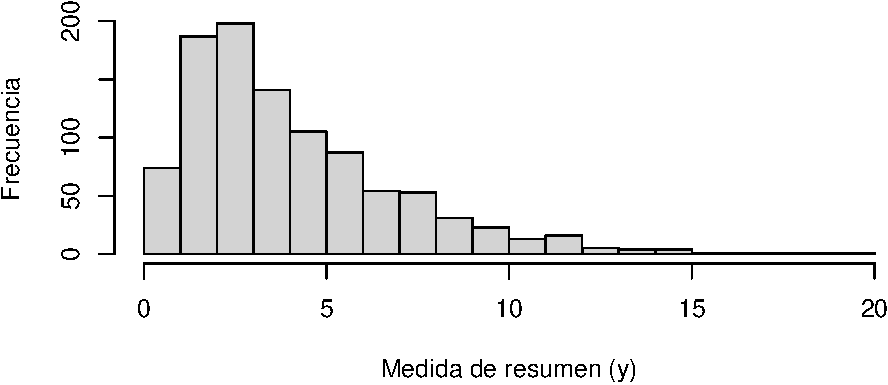
\includegraphics{EH-CEPAL_files/figure-latex/unnamed-chunk-1-1.pdf}
\caption{\label{fig:unnamed-chunk-1}Patrón de respuesta MCAR}
\end{figure}

\begin{itemize}
\tightlist
\item
  \textbf{Aleatoria dependiente de covariables} \emph{(Missing At Random - MAR)}: cuando la probabilidad de que un individuo responda depende de algunas covariables auxiliares, pero no depende de la característica de interés. Por ejemplo, en una encuesta de fuerza laboral, la ausencia de respuesta puede depender de la edad del respondientes, o del sexo, o incluso del nivel económico del individuo, pero no depende de su clasificación laboral. El siguiente gráfico muestra que el patrón de ausencia de respuesta podría ser MAR puesto que el sexo y la zona del respondiente están influenciando el porcentaje de respuesta, aunque no el estado de ocupación.
\end{itemize}

\begin{figure}
\centering
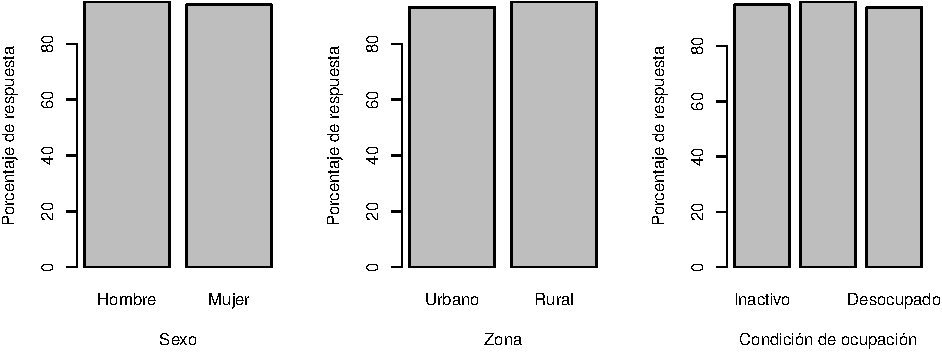
\includegraphics{EH-CEPAL_files/figure-latex/unnamed-chunk-2-1.pdf}
\caption{\label{fig:unnamed-chunk-2}Patrón de respuesta MAR}
\end{figure}

\begin{itemize}
\tightlist
\item
  \textbf{No aleatoria} \emph{(Missing Not At Random - MNAR)}: cuando la ausencia de respuesta depende de la característica de interés. Por ejemplo, en la encuesta de fuerza laboral, es posible que los no respondientes dependan de su clasificación laboral. En este caso puede suceder que los desocupados sean los que sistemáticamente no respondan la encuesta. El siguiente gráfico muestra indicios de que el patrón de respuesta es MNAR puesto que la condición de ocupación es la que influencia el porcentaje de respuesta.
\end{itemize}

\begin{figure}
\centering
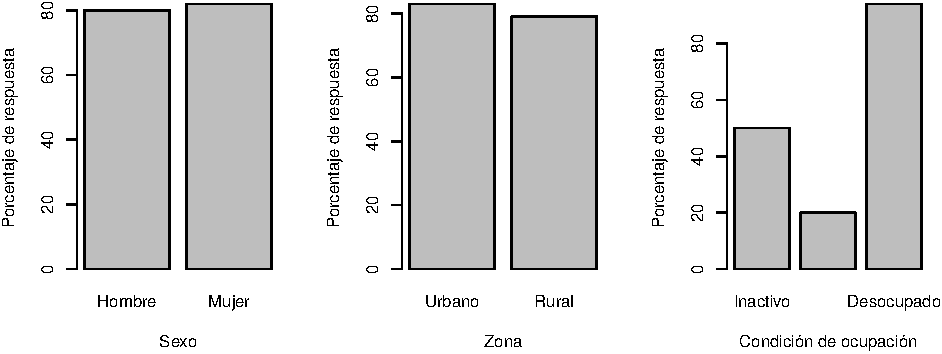
\includegraphics{EH-CEPAL_files/figure-latex/unnamed-chunk-3-1.pdf}
\caption{\label{fig:unnamed-chunk-3}Patrón de respuesta MNAR}
\end{figure}

Nótese que a pesar de que se hayan tomado las medidas de ajuste necesarias en el diseño de la encuesta, cuando ya ha terminado el proceso de recolleción de infomración, se debe lidiar con la ausencia de respuesta para evitar sesgos y aumentar la precisión de la encuesta. La literatura especializada examina dos metodologías diferentes pero complementarias en el ejercicio de una encuesta: la prevención de la ausencia de respuesta (antes de que ocurra) y las técnicas de estimación necesarias para tener en cuenta la ausencia de respuesta de manera apropiada en el proceso de inferencia, después de la recolección de los datos. Si el mecanismo de ausencia de respuesta se asume MCAR, es posible contemplar en el proceso de inferencia únicamente a aquellas unidades que tienen registros completos y eliminar de la base de datos a aquellas unidades que no contestaron (\emph{list-wise deletion}). A pesar de que este tipo de análisis es simple, para evitar subestimaciones de los parámetros de interés, se debe realizar un ajuste de los factores de expansión inducidos por el diseño muestral, que originalmente fue planeado con un tamaño de muestra más grande que el efectivo. De esta forma, es posible suponer que la muestra de respondientes corresponde a una submuestra completamente aleatoria de la población y utilizar los principios de los diseños en dos fases. \textcite[capítulo 11]{Heeringa_West_Berglund_2010} afirman que este tipo de análisis, además de inducir posibles sesgos si el supuesto MCAR no se cumple, reduce la eficiencia de la inferencia debido al decremento del tamaño de muestra efectivo. Por lo tanto, en la mayoría de encuestas, este supuesto no se asume y se realiza un ajuste adicional después de que ha ocurrido la ausencia de respuesta. Es por esto que \textcite[sección 15.5]{Sarndal_Swensson_Wretman_2003} afirman que las principales técnicas para tratar la ausencia de respuesta son el ajuste a los pesos de muestreo y la imputación. El ajuste por ponderación implica aumentar los pesos aplicados en la estimación de los valores y de los encuestados para compensar los valores que se pierden debido a la ausencia de respuesta, mientras que la imputación implica la sustitución de los valores faltantes por valores artificiales.

Siguiendo la notación en \textcite{Sarndal_Lundstrom_2006}, consideramos una muestra seleccionada \(s\) de unidades de interés; como resultado del proceso de observación se denota a \(r\) como el conjunto de unidades que respondieron a uno o más de los \(I\) variables de interés. Una unidad que no respondió a ninguna de las variables del estudio pertenecerá entonces al conjunto \(s−r\). Así mismo, el conjunto de unidades que respondieron a una variable particular es denotado por \(r_i\). Observe que, en general, todos los \(r_i\) tendrán tamaños diferentes y además estarán contenidos en \(r\); de esta forma, se tiene que:

\[
r_i\subseteq r \subseteq s
\]

La siguiente figura ilustra cómo, después de la recolección de datos, hay individuos que no respondieron a una o todas las variables de la encuesta. En esta ilustración, las unidades están representadas por las filas y las variables por las columnas. Observe que lo primeros tres individuos contestaron a todas las preguntas del cuestionario; el cuarto individuo no contestó las últimas dos preguntas; el quinto individuo no contestó ni la primera ni la última pregunta; el sexto individuo no contesto a la tercera pregunta; y así sucesivamente, hasta llegar a los últimos dos individuos quienes no contestaron a ninguna pregunta del cuestionario. Para este ejemplo particular, se observa que \(I=8\), \(n=\#(s)=14\), \(\#(r_1)=10\), \(\#(r_1)=10\), \(\#(r_2)=9\), \(\#(r_3)=10\), \(\#(r_4)=10\), \(\#(r_5)=11\), \(\#(r_6)=10\), \(\#(r_7)=10\), \(\#(r_8)=8\) y \(\#(r_8)=12\).

\begin{figure}
\centering
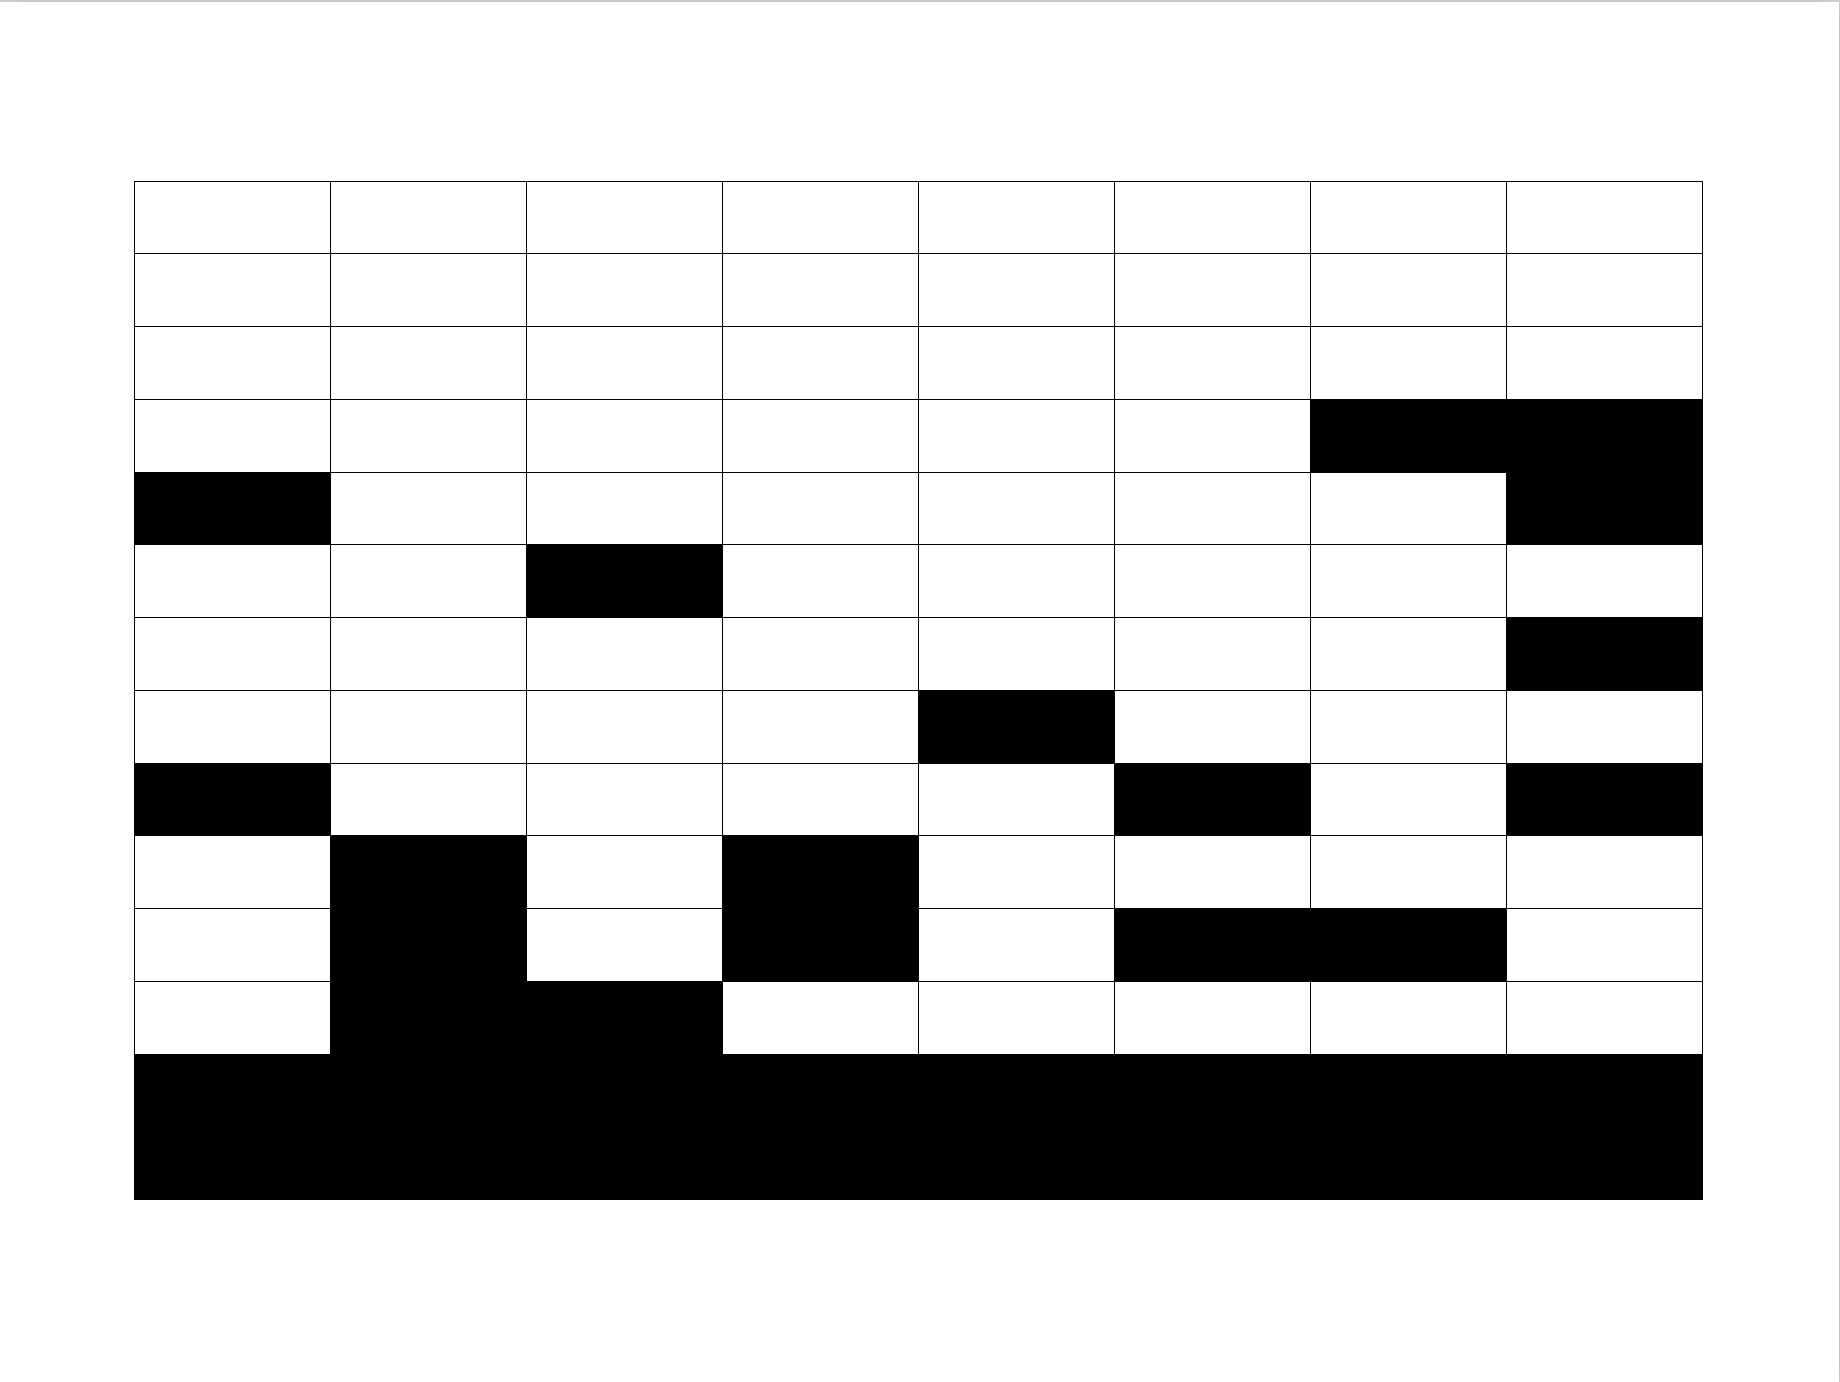
\includegraphics[width=3.125in,height=\textheight]{Pics/j1.png}
\caption{\emph{Un conjunto de datos después del proceso de observación.}}
\end{figure}

Al lidiar con la ausencia de respuesta podemos distinguir varios enfoques para la estimación. El más extremo se conoce como el \textbf{enfoque de eliminación}, en donde se conservan para el análisis únicamente aquellas unidades que han respondido a todas y cada una de las pregutnas del cuestionario; es decir que aqueelas unidades que no respondierona al menos una pregunta serán eliminadas del análisis. Note que en este enfoque sólo las unidades del conjunto \(r\) se consideran para el análisis posterior. Por supuesto, en general, esto no es aconsejable puesto que trae problemas de sesgo, dado que las unidades que contestaron todo el cuestionario generalmente difieren de forma estructural de las unidades que no contestaron; además trae problemas de eficiencia estadística, puesto que el tamaño de la muestra efectiva, después de la eliminación de unidades, será insuficiente para garantizar los mínimos requeridos en la inferencia. La siguiente figura muestra que, teneindo en cuenta el ejemplo anterior, solo tres unidades serían tenidas en cuenta para el análisis de la información, mientras que nueve unidades, que no contestaron al menos una pregunta, más las tres unidades que no contestaron ninguna pregunta, serían eliminadas del análisis estadístico. Es decir, la mayoría de unidades de la muestra incial serían descartadas.

\begin{figure}
\centering

\includegraphics[width=3.125in,height=\textheight]{Pics/j2.png}
\caption{\emph{Enfoque de eliminación: todas las unidades que no pertencen a \(r\) con eliminadas.}}
\end{figure}

El segundo enfoque se denomina \textbf{imputación total}, y se trata de imputar todos los valores faltantes del conjunto de observaciones. Es decir, los valores de las personas que no respondieron al menos a una variable en todo el cuestionario serán imputados. En este enfoque, la imputación se utiliza para tratar la ausencia de respuesta del ítem y la ausencia de respuesta de la unidad al mismo tiempo. La siguiente figura muestra un ejemplo de las unidades que serían consideradas para el análisis después de la imputación. Nótese entonces que las tres unidades que respondieron todas las preguntas del cuestionario entran al análisis sin nigun ajuste; mientras que las nueve unidades que no respondieron a todo el cuestionario entran al análisis habiendose imputado las celdas correspondientes a la ausencia de respuesta; además, las dos unidades que no respondieron ninguna pregunta del cuestionario también entran al análisis puesto que todas sus respuestas fueron imputadas. Luego, en este enfoque todas las unidades en el conjunto \(s\) se consideran para el análisis posterior.

Observe que si \(y_k\) es una observación faltante y es imputada, entonces \(\hat{y}_k\) denotará el valor imputado obtenido por cualquiera de los métodos de imputación que se describirán más adelante. Luego, como en este enfoque se imputan valores para todas las observaciones faltantes, ya sea por unidad o por no respuesta del ítem, se tendrá un conjunto de datos completos con los valores

\[
y_{\circ \  k} = 
\begin{cases}
y_k, \ \text{for $k \in r_i$} \\
\hat{y}_k, \ \text{for $k \in s - r_i$}
\end{cases}
\]

\begin{figure}
\centering
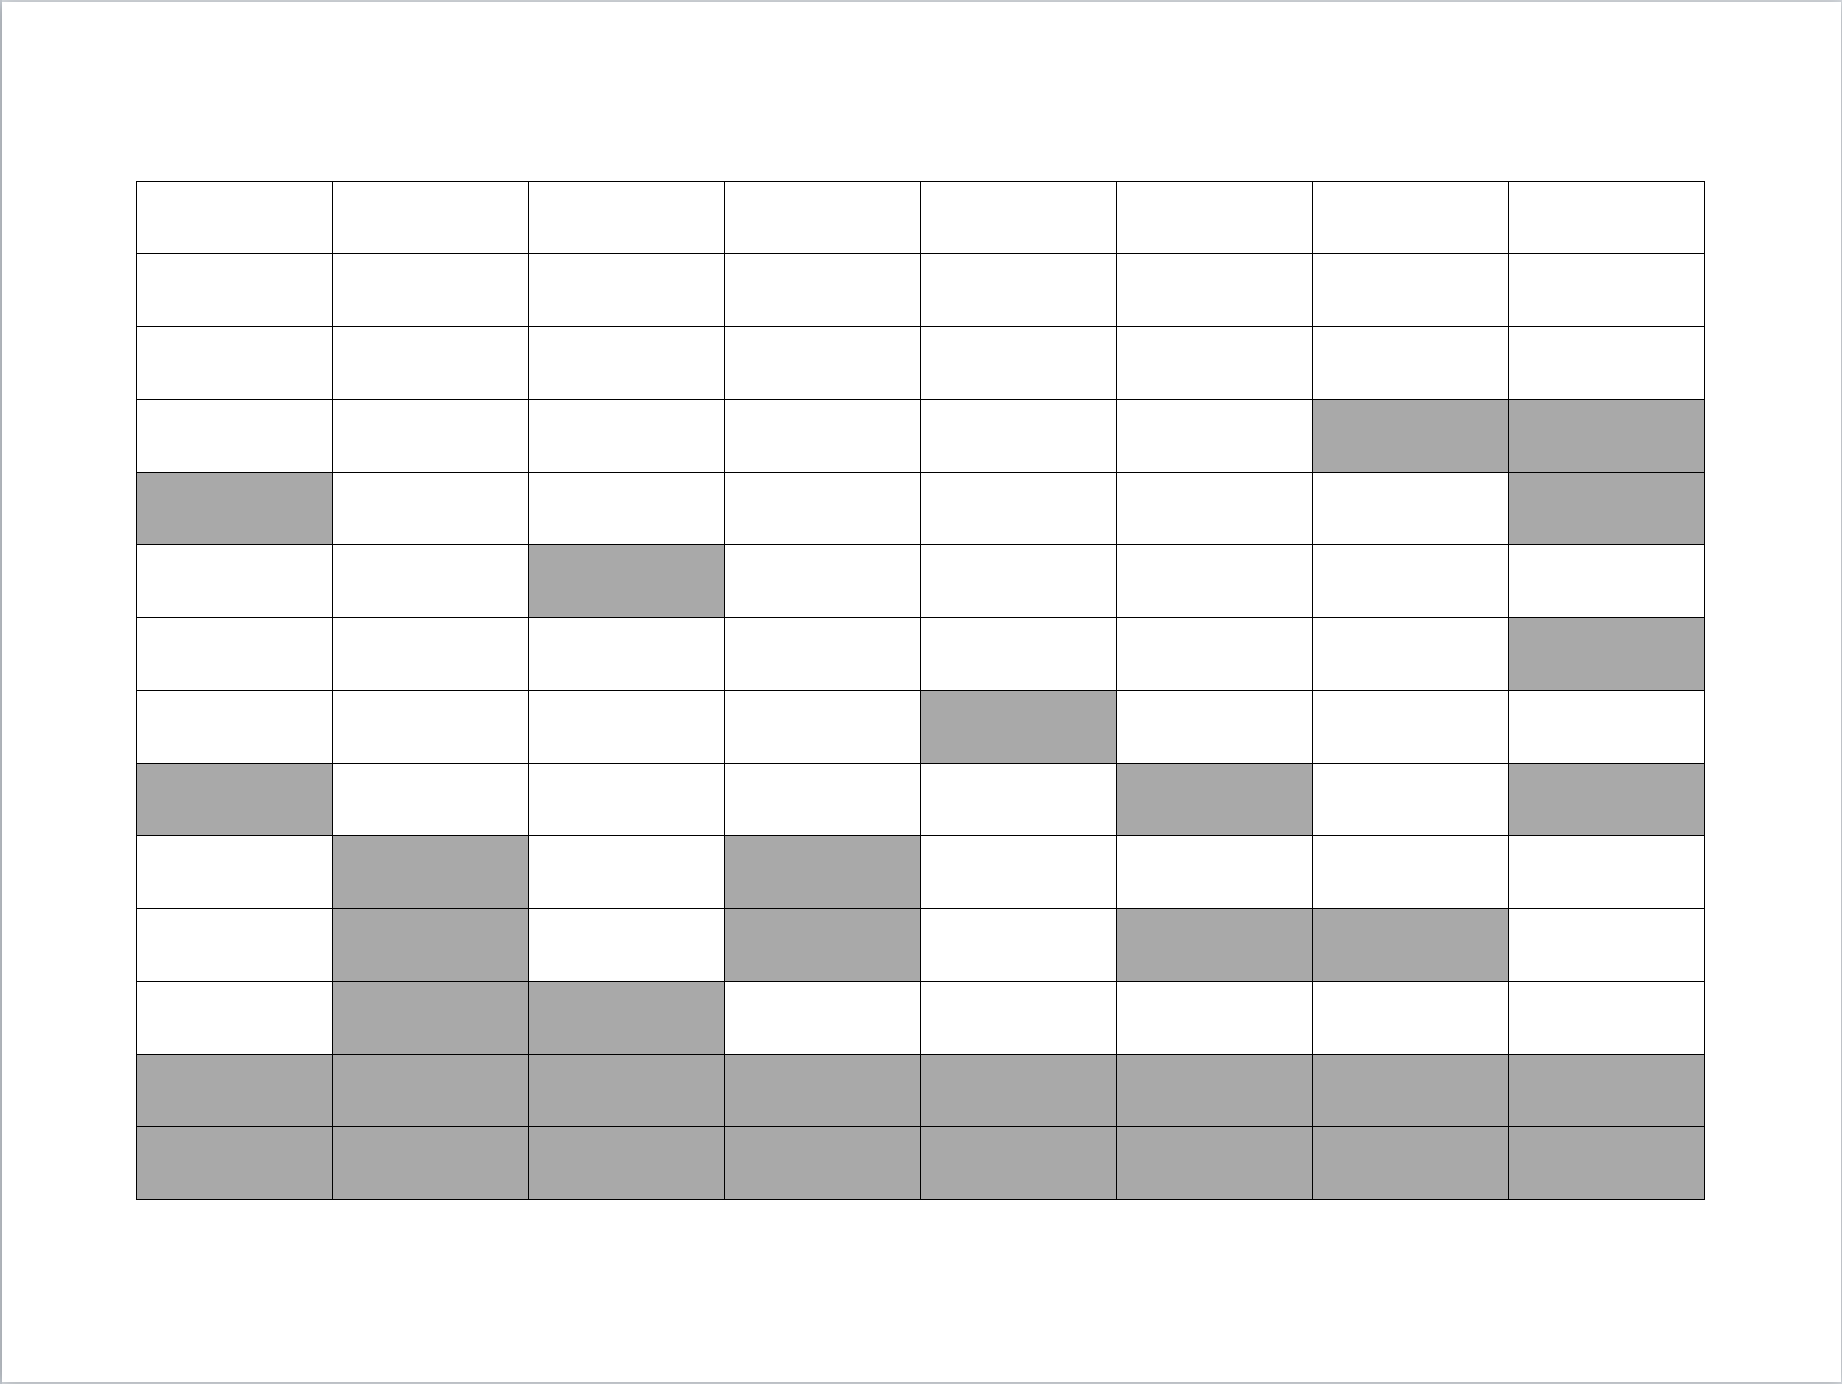
\includegraphics[width=3.125in,height=\textheight]{Pics/j3.png}
\caption{\emph{Imputation total: todas las unidades que no están en \(s-r\) son imputadas (las celdas en gris indican los valores que fueron imputados).}}
\end{figure}

El tercer enfoque se denomina \textbf{ponderación total} y se utiliza para cada variable de interés en el estudio, una a la vez. En este enfoque nunca se utiliza la imputación, puesto que existirán tantos conjuntos de pesos y ponderaciones como variables con valores faltantes. Para este esquema, se utilizan pesos \(w_k^{(i)}\) para cada variable \(i \in I\) que compensan la ausencia de respuesta de la unidad. Si todos los \(r_i\) son diferentes, cada variable de estudio requirá un peso diferente. Siguiendo con los ejemplos de las ilustraciones, se nota que la primera variable del cuestionario fue respondida por 10 personas, y cuatro personas no respondieron esta pregunta. Por lo tanto, en este enfoque se crearán pesos \(w_k^{(1)}\) para cada \(k\in s\) que ponderen satisfactoriamente la información recolectada en esta variable. Sin emabrgo, este conjunto de pesos no será único, puesto que, en particular, la segunda variable del cuestionario fue respondida por nueve personas, y tres personas no respondieron esta pregunta. Por lo tanto, en este enfoque se crearán pesos \(w_k^{(2)}\) para cada \(k\in s\) que ponderen esta información recolectada en esta variable. Nótese que en general \(w_k^{(1)} \neq w_k^{(2)}\) y, por ende, cada una de las \(I=8\) variables del estudio tendrá su propio conjunto de ponderadores.

\begin{figure}
\centering
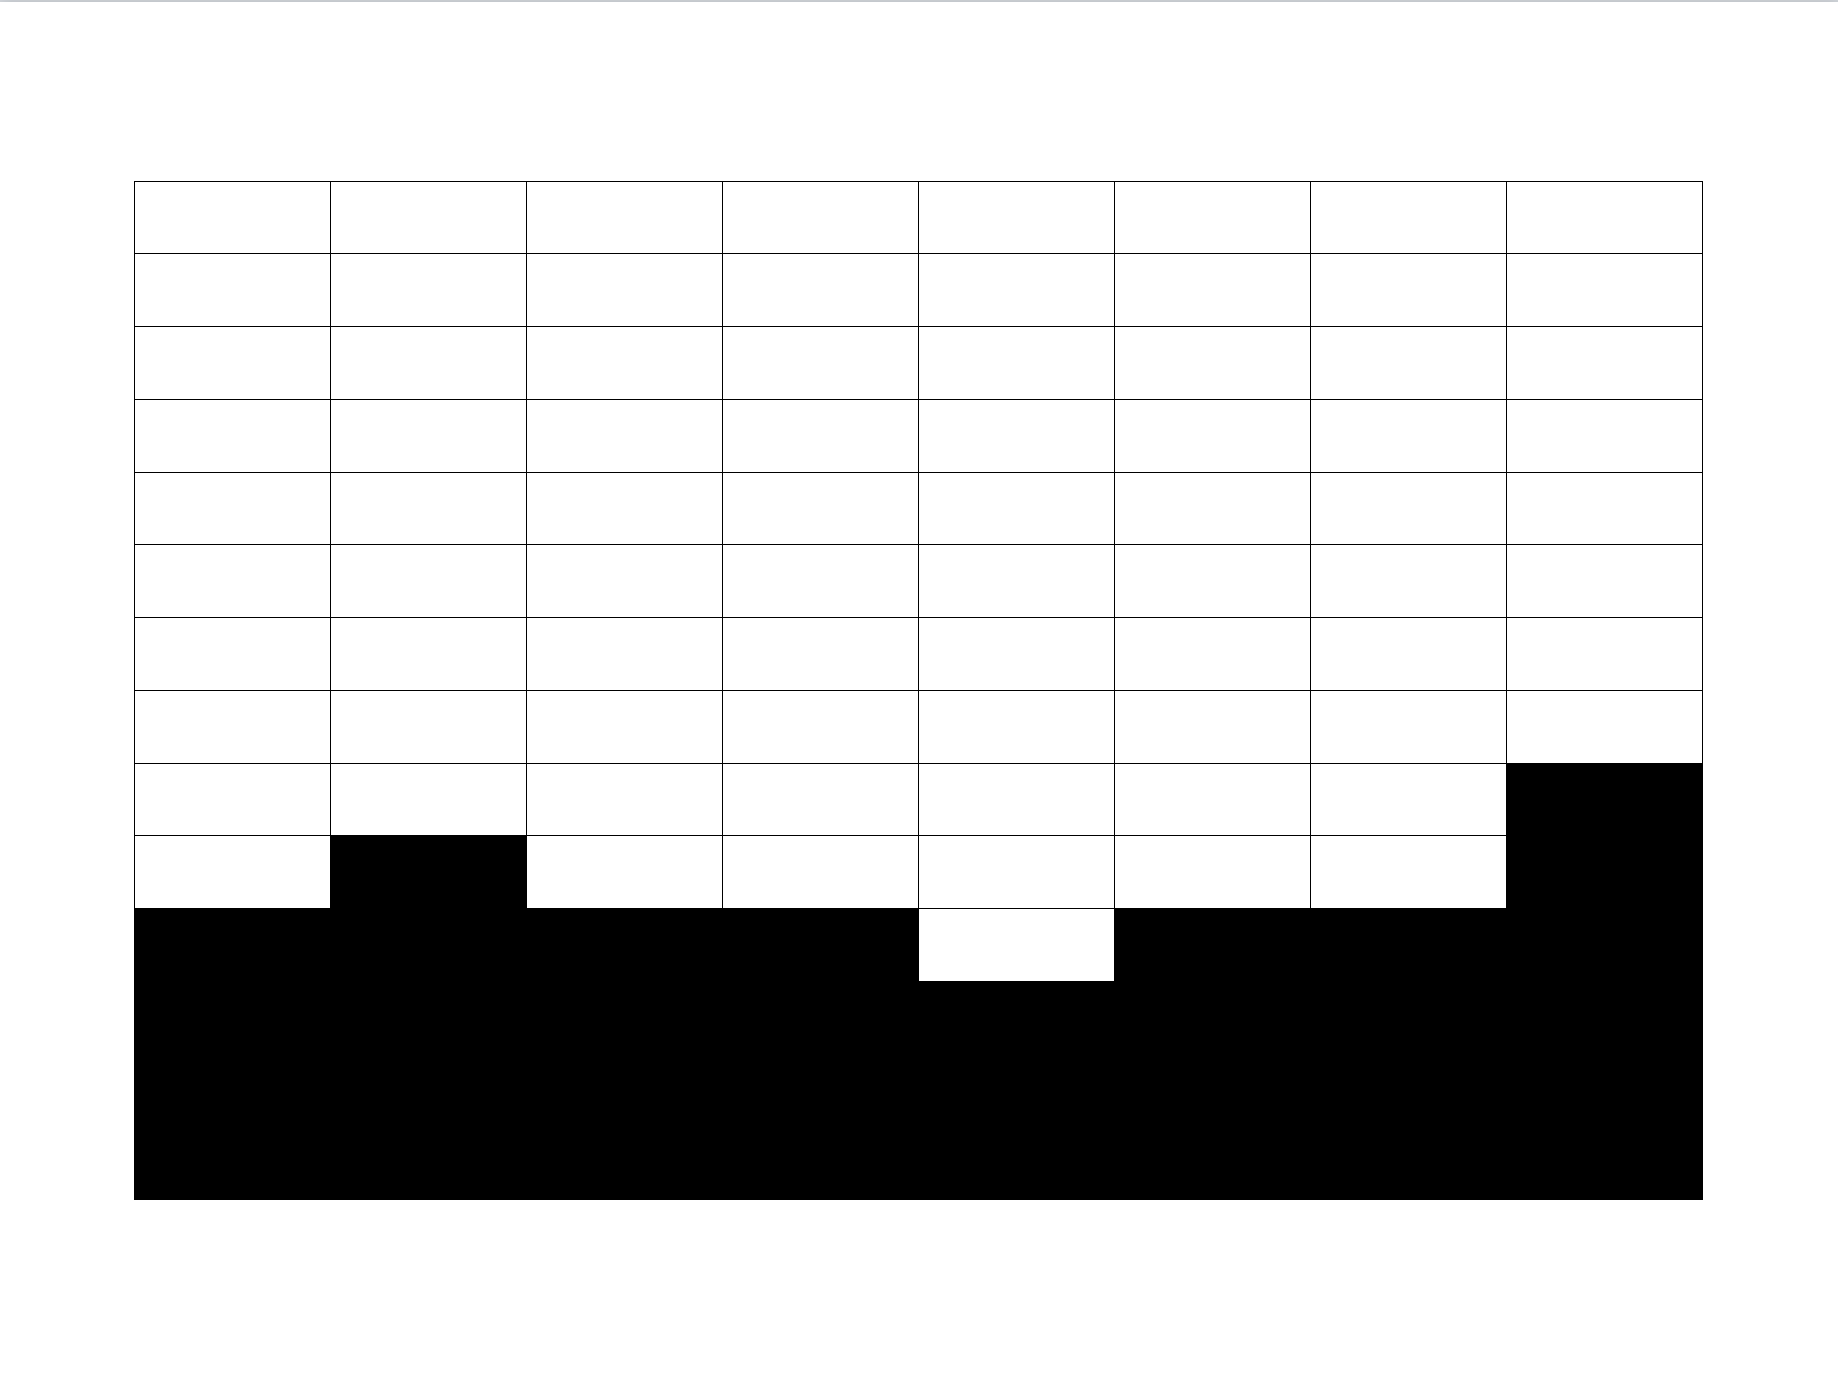
\includegraphics[width=3.125in,height=\textheight]{Pics/j4.png}
\caption{\emph{Ponderación total: cada variable tendrá un conjunto de pesos diferente. No se utiliza ningún método de imputación.}}
\end{figure}

Por último, el enfoque recomendado es una combinación de los procediemintos de imputación y ponderación y se conoce como \textbf{enfoque combinado} que imputa los valores de las celdas ausentes para los individuos que tienen al menos un valor faltante, exceptuando a aquellos que tienen todos los valores faltantes. De esta forma, los individuos que no contestaron ninguna pregunta del cuestionario son eliminados del análisis, mientras que los restantes serán considerado en el análisis con sus respuestas originales o con la imputación de las celdas vacías. En resumen, este enfoque implica que la imputación se utilice para tratar sólo la ausencia de respuesta del ítem, mientras que la ponderación se utilice únicamente para tratar la ausencia de respuesta del individuo. Retomando el ejemplo, el siguiente gráfico permite observar que los dos últimos individuos de la muestra fueron totalmente descartados puesto que no contestaron ninguna pregunta del cuestionario; además, para la primera variable, los valores del quinto y noveno individuo fueron imputados. De la misma manera, para la segunda variable, los valores de lso individuos 10, 11 y 12, fueron imputados; y así sucesivamente, hasta llegar a la última variable en donde los valores de los indivioduos tres, cuatro, seis y ocho fueron imputados.

\begin{figure}
\centering
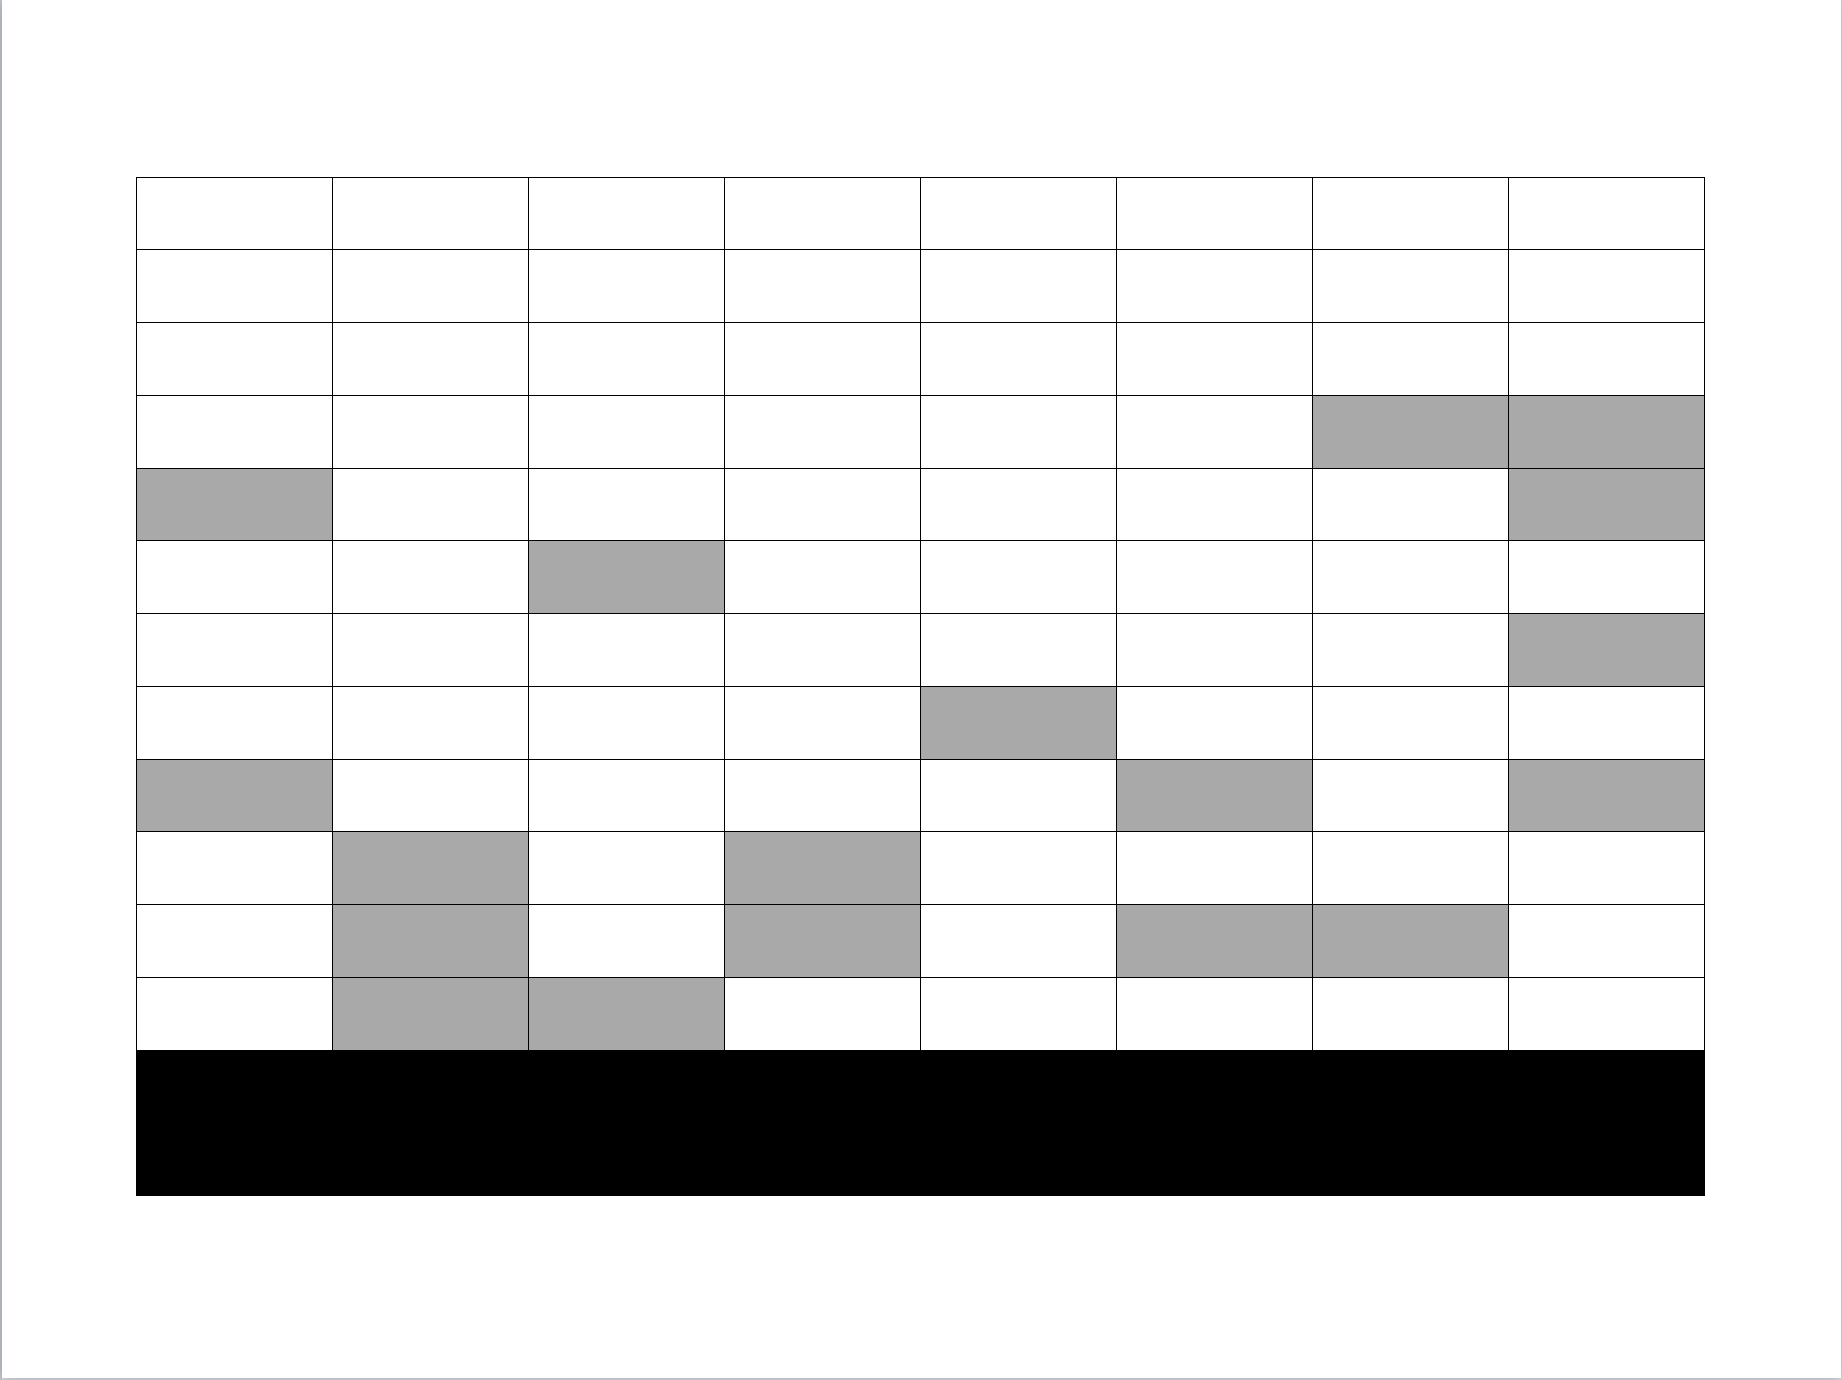
\includegraphics[width=3.125in,height=\textheight]{Pics/j5.png}
\caption{\emph{Enfoque combinado: las unidades que no respondieron a ningún ítem son eliminadas del análisis y los respondientes parciales son imputados.}}
\end{figure}

En la realidad de las encuestas de hogares, lo más común es encontrar que se presente ausencia de respuesta tanto de unidad como de ítem. En estos casos, se aconseja imputar primero y luego descartar los individuos que no contestaron a niguna pregunta, de esta forma al final se obtendrá una matriz de datos rectangular completa. Por tanto, el conjunto de datos completados (originales o imputados) para la variable \(y\) es \(\{y_{\circ \  k}: k\in r\}\), en donde

\[
y_{\circ \  k} = 
\begin{cases}
y_k, \ \text{for $k \in r_i$} \\
\hat{y}_k, \ \text{for $k \in r - r_i$}
\end{cases}
\]

\hypertarget{imputacion}{%
\section{Imputación}\label{imputacion}}

El término imputación se refiere al conjunto de técnicas por las cuales los valores faltantes en una o más variables se reemplazan con infrmación plausible con el objetivo de lograr valores sustitutivos en una base de datos que pueda ser analizada posteriormente. Este proceso introduce un nuevo elemento de error, conocido como el error de imputación, debido a la incertidumbre que introducen los valores no observados. Cuando se tiene ausencia de respuesta por ítem, las técnicas de imputación se prefieren antes que la utilización de los esquemas de ponderación en la muestra. De esta manera, es posible crear un conjunto completo y rectangular de datos mediante la imputación de los valores faltantes, puesto que después de realizar la imputación, se espera que todos los valores del cuestionario de un individuo contengan información y no exista ningún vacío. Para lograr la sutitución de los valores faltantes con infomración plausible, es posible encontrar donantes apropiados, en la misma muestra que se ha conseguido, definidos como respondientes que comparten características demográficas similares con el individuo que no respondió. Por lo tanto, la información del respondiente donante (o una función de estos valores) se copiará en las celdas vacías del no respondiente. Para encontrar los donantes es posible realizar un análisis estadístico con base en métodos de clasificación. Dentro de los métodos de imputación más usados en encuestas de hogares se encuentran los siguientes:

\begin{itemize}
\tightlist
\item
  Imputación promedio (\emph{mean value imputation}) que utiliza la media de la variable (dentro de las UPM o en un subconjunto apropiado de datos). En este caso, si se encuentra un valor faltante, inmediantamente será reemplazado por el promedio de los datos de los respondientes en esta variable.
\item
  Imputación por paquete caliente (\emph{hot deck imputation}) que reemplaza los valores faltantes por los valores de un donante que es un respondiente de la encuesta en el mismo levantamiento. En este caso, el valor faltante es reemplazado por la información del individuo escogido de antemano.
\item
  Imputación por paquete frío (\emph{cold deck imputation}) que reemplaza los valores faltantes por los valores de un donante que es un respondiente de encuesta en un levantamiento anterior. En este caso, el valor faltante es reemplazado por la información auxiliar de un individuo escogido de encuestas anteriores.
\item
  Imputación estadística que se apoya en un modelo (de regresión, generalmente) en donde la variable dependiente es aquella que se quiere imputar y las covariables se derivan del restante conjunto de datos. En este caso, el valor faltante es reemplazado por la predicción (o una función) del modelo ajustado con la información en la muestra.
\end{itemize}

Como se mencionó anteriormente, cuando se trata de imputación, se pueden definir dos tipos de métodos. La imputación de la unidad completa, que se produce cuando toda la información de un individuo es imputada, y la imputación del ítem, que se da cuando un único valor de un individuo es imputado. Observe que la imputación de la unidad se utiliza para hacerle frente a la ausencia de respuesta de la unidad, cuando no hay datos para el individuo, mientras que la imputación del ítem se utiliza para la no respuesta del ítem, cuando no todos los valores se proporcionan para un individuo, pero algunos sí.

La imputación se realiza a menudo en grupos no traslapados \(g= 1, \ldots, G\), donde la unión de \(s_1, \ldots, s_G\) equivale a la muestra completa \(s\). Se pueden utilizar diferentes métodos para cada grupo, pero dentro de cada grupo se debe utilizar el mismo método de imputación. Esto se debe a que pueden existir diferentes covariables disponibles para cada grupo. Cuando la disponibilidad de las variables auxiliares (covariables) es limitada, es posible considerar una jerarquía de métodos de imputación. De esta forma, para los grupos con más información disponible, es posible utilizar métodos más sofisticados de imputación; mientras que para grupos con menos información auxiliar disponbible, se deben usar métodos de imputación más simples. \textcite{Sarndal_Lundstrom_2006} presentan una discusión acerca del uso de esta técnica en combinación con los estimadores utilizados en las encuestas de hogares que proveen estadísticas oficiales. A continuación, se presenta una compilación no exhaustiva de algunos de los principales métodos de imputación que se utilizan en las encuestas de hogares.

\hypertarget{imputacion-por-regresion}{%
\subsubsection*{Imputación por regresión}\label{imputacion-por-regresion}}
\addcontentsline{toc}{subsubsection}{Imputación por regresión}

En este método determinístico, el valor imputado para el valor faltate \(y_k\) se calcula utilizando una regresión lineal.
\[\hat{y}_k = \mathbf{x}_k \hat{\boldsymbol{\beta}}_i\]
Donde,
\[
\hat{\boldsymbol{\beta}}_i = (\sum_{r_i} a_k\mathbf{x}_k\mathbf{x}_k')^{-1}
\sum_{r_i} a_k\mathbf{x}_ky_k
\]
El vector de coeficientes de regresión \(\hat{\boldsymbol{\beta}}_i\) se produce a partir de un ajuste de regresión múltiple utilizando los datos \((y_k, \mathbf{x}_k)\) disponibles para cada unidad \(k \in r_i\) con pesos \(a_k\) especificados adecuadamente. Nótese que, en general, las predicciones del modelo de regresión no necesariamente serán valores observados en algún otro individuo de la muestra. Por lo tanto, este método inducirá valores imputados que no han sido observados en la encuesta. Además, se deberán generar tantos modelos de regresión como variables con valores faltantes existan.

\hypertarget{imputacion-de-razon}{%
\subsubsection*{Imputación de razón}\label{imputacion-de-razon}}
\addcontentsline{toc}{subsubsection}{Imputación de razón}

Un caso especial del anterior método se da cuando solo se tiene acceso a una sola covariable (positiva) \(\mathbf{x}_k = x_k\), y definiendo \(a_k = \frac{1}{x_k}\). En este caso, la estimación del coeficiente de regresión será

\[
\hat{{\beta}}_i = \frac{\sum_{r_i}y_k}{\sum_{r_i}x_k} = R_i
\]

Y por tanto, la imputación para el valor faltante se convierte en

\[\hat{y}_k = x_k \hat{\beta}_i = x_k \frac{\sum_{r_i}y_k}{\sum_{r_i}x_k} = x_k R_i\]

Este método se utiliza a menudo cuando la misma variable se mide en dos momentos diferentes en la misma encuesta. Por ejemplo, si \(y\) indica la variable de estudio en el momento actual, \(x\) indica la variable en el punto de tiempo anterior, entonces el coeficiente utilizado para la imputación es la relación entre los dos puntos en el tiempo.

\hypertarget{imputacion-de-promedio}{%
\subsubsection*{Imputación de promedio}\label{imputacion-de-promedio}}
\addcontentsline{toc}{subsubsection}{Imputación de promedio}

El caso más sencillo de la imputación por regresión se da cuando \(a_k = x_k = 1\) para todo \(k \in r_i\). En este escenario, el valor imputado se convierte en

\[\hat{y}_k  = \frac{\sum_{r_i}y_k}{\sum_{r_i}1}= \bar{y}_{r_i}\]

Por lo tanto, todos los valores faltantes recibirán el mismo valor imputado, que es justamente el promedio de la variable en el conjunto de respondientes. Nótese que no se requiere de ninguna información adicional en este método.

\hypertarget{el-vecino-mas-cercano}{%
\subsubsection*{El vecino más cercano}\label{el-vecino-mas-cercano}}
\addcontentsline{toc}{subsubsection}{El vecino más cercano}

Si asumimos que valores similares de \(x\) producirán valores similares de \(y\), podemos ``pedir prestado'' un valor de \(y\) para imputar el valor faltante de un ``vecino'' con valores similares en \(x\). En este caso, el valor imputado para la unidad \(k\) está dado por

\[\hat{y}_k = y_{l(k)}\]

Dónde \(l(k)\) es el ``elemento donante'', determinado al minimizar una ecuación de distancia. Enn el caso más simple, para una sola covariable de imputación \(x_k\), la distancia entre los posibles donantes \(l\) a la unidad \(k\) es:

\[
D_{lk} = |x_k - x_l|
\]

El donante \(l\) al elemento \(k\) es aquel individuo en el conjunto \(r\) con la menor distancia \(D_{lk}\) entre todos los posibles elementos \(l\in r\). Para el caso en donde se contemple más de una covariable de imputación, es posible considerar la siguiente distancia

\[
D_{lk} = \left( \sum_{j=1}^J h_j (x_{jk} - x_{jl})^2 \right)
\]

En donde \(h_j\) se utiliza para ponderar adecuadamente cada una de las \(J\) covariables de la matriz de imputación.

\hypertarget{imputacion-hot-deck}{%
\subsubsection*{Imputación Hot Deck}\label{imputacion-hot-deck}}
\addcontentsline{toc}{subsubsection}{Imputación Hot Deck}

La imputación por regresión y el vécino más cercano son métodos que asumen una fuerte relación entre la variable de interés \(y\) y las covariables \(\mathbf{x}\). Sin embargo, en algunas aplicaciones esta relación no se puede establecer fácilmente, y no es plausible validar los supuestos de modelación que otros métodos requieren. Por lo tanto, en este tipo de técnica, el valor imputado para el individuo \(k\) está dado por:

\[\hat{y}_k = y_{l(k)}\]

Donde el valor imputado \(y_{l(k)}\) es proporcionado por un donante seleccionado aleatoriamente del conjunto de datos de la variable de interés. Este método no se recomienda cuando existen mejores opciones, ya que no se cuenta con información auxiliar para determinar un buen sustituto.

\hypertarget{imputacion-multiple}{%
\subsubsection*{Imputación múltiple}\label{imputacion-multiple}}
\addcontentsline{toc}{subsubsection}{Imputación múltiple}

Cuando existe información auxiliar que permita relacionar las covariables con la variable de interés, es posible establecer mejores modelos que no solo mantienen el insesgamiento de la inferencia, sino que estiman con bastante precisión el error de muestreo. Con respecto a esta última categoría de imputación, es posible completar el conjunto de datos utilizando información auxiliar de los respondientes en la encuesta (o encuestas anteriores, si se trata de un diseño rotativo) y la información disponible a nivel de la población para predecir los valores faltantes usando un modelo de regresión. Una de las técnicas más robustas es la imputación múltiple que consiste en formular un modelo probabilístico entre la variable de interés y las covariables disponibles en la encuesta \autocite{Rubin_1987}. Suponga que este modelo es de la forma

\[y_k = f(\mathbf{x_k},\boldsymbol{\beta}) + \varepsilon_k \]
En donde \(\varepsilon_k\) es un término de error aleatorio. Una vez formulado el modelo, y debido a la naturaleza estocástica de \(\varepsilon_k\), es posible generar \(Q>1\) realizaciones de la variable de interés para los registros faltantes; esto se logra de manera muy sencilla, simulando \(Q\) valores del término de error. De esta forma, se generan \(Q\) conjuntos de datos completos. Para cada conjunto de datos, se generarán \(Q\) estimaciones de interés que luego se promedian para obtener una estimación puntual.

\hypertarget{ejemplo-imputacion-en-una-encuesta-de-ingresos-y-gastos}{%
\subsection{Ejemplo: imputación en una encuesta de ingresos y gastos}\label{ejemplo-imputacion-en-una-encuesta-de-ingresos-y-gastos}}

Una vez que se ha discutido acerca de los propósitos de la imputación en una encuesta de hogares, se debe escoger un método (o métodos) de imputación y una vez establecido el mecanismo de imputación, generar el conjunto de datos rectangular y completo. En esta sección analizaremos, a la luz de las particularidades de una encuesta de hogares de ingresos y gastos, los pasos que se deben surtir para completar un proceso de imputación. Por sus características, este tipo de encuestas presenta tasas elevadas de ausencia de respuesta de ítem, aunque también de individuo.

En general, el levantamiento común de este tipo de encuestas se centra en un trabajo de campo masivo que visita al hogar en varias ocasiones, pidiéndole al respondiente que diligencie sendos cuestionarios, y registre toda la información asociada al gasto y a los ingresos del hogar, durante un periodo de al menos dos semanas. Por supuesto, para que esto pueda realizarse, es necesario contar con la colaboración activa de todos los miembros del hogar. En el mejor de los casos, el encuestador habrá visitado varias veces el domicilio del hogar en el periodo de observación y tendrá un formulario totalmente diligenciado. Sin embargo, en muchas otras ocasiones, a pesar del seguimiento exhaustivo del encuestados, no se obtendrá el gasto de la totalidad de las categorías de la encuesta, sino que se obtendrá infomración parcial que se transformará en celdas vacías por la ausencia de respuesta. En el peor de los casos se obtendrán cuestionarios diligenciados en porcentaje tan bajo, que al final serán declarados como faltantes, lo cual se transforma en ausencia de respuesta de ese hogar.

El siguiente ejemplo trata de ilustrar de manera escueta cómo se debería realizar el procedimiento de imputación en una encuesta de ingresos y gastos. El lector encontrará varios pasos en esta metodología, puesto que antes de imputar las variables de interés, es ncesario conocer qué covariables se relacionan fuertemente con las variables que se quieren imputar. Además de eso, es necesario primero imputar todas las covariables en primer lugar y reemplazar sus valores faltantes con información plausible que pueda ser utilziada en los modelos que se ajusten. Suponga que, para el conjunto de hogares que se consideró con fines de imputación, se observaron al menos las siguientes variables:

\begin{itemize}
\tightlist
\item
  Tamaño del hogar.
\item
  Número de hombres y mujeres dentro del hogar.
\item
  Número de niños y adultos en el hogar.
\item
  Edad del jefe de hogar.
\item
  Estado de ocupación del jefe de hogar.
\item
  Grado educativo más alto del jefe de hogar.
\item
  Número de personas empleadas en el hogar.
\end{itemize}

El camino que se seguirá en este ejemplo será primero la imputación de los ingresos, como principal covariable del gasto y del consumo. Una vez que se imputaron las covariables, el segundo paso de este proceso se relaciona con la imputación de los filtros, que son las preguntas que se realizan para conocer si un hogar ha adquirido un bien o servicio específico. El resultado de este paso produjo el tercer paso dedicado a la imputación de los valores de gasto anualizados en cada unidad. Esta serie de pasos metodológicos ha sido recomendados por diferentes agencias de estadística, incluyendo institutos y oficinas nacinoales de estadística. Por ejemplo, \textcite{Hayes_Watson_2009} y \textcite{Sun_2010} siguen esta metodología en el \emph{Australian Bureau of Statistics} para imputación en la encuesta \emph{Household, Income and Labour Dynamics in Australia (HILDA)}

\hypertarget{imputacion-del-ingreso}{%
\subsubsection*{Imputación del ingreso}\label{imputacion-del-ingreso}}
\addcontentsline{toc}{subsubsection}{Imputación del ingreso}

En primer lugar, debe ser notado que tanto teórica como empíricamente, los ingresos han demostrado ser un potente predictor de los gastos \autocite{Starick_Watson_2011}. Si la base de datos contiene hogares que reportaron un ingreso nulo en todo el año, es posible que esos valores se consideren como faltantes porque se asume que los hogares no deben tener ingresos nulos durante todo un año. Además, los hogares con ingresos superiores a un límite también pueden ser considerados como valores atípicos y luego ser imputados.

La imputación del ingreso está basada en un enfoque de modelos predictivos y la técnica que se podría utilizar para imputar esta covariable es la del vecino más cercano con regresión. De esta forma, se define un modelo lineal para las unidades encuestadas y luego se estiman los coeficientes de regresión para obtener un valor pronosticado que se computa para las unidades que faltan. Así, para cada unidad con información faltante en el ingreso, se identifica un solo donante que corresponderá al hogar cuyo ingreso disponible es más cercano a la predicción del modelo de regresión. Por ende, todos los componentes de los ingresos son imputados por el donante. El modelo lineal se describe como se indica a continuación y la predicción de los ingresos para los hogares faltantes se calcula utilizando una regresión lineal.

\[\tilde{y}_k = \mathbf{x}_k \hat{\boldsymbol{\beta}}_i\]

Donde, \(\tilde{y}_k\) es el valor pronosticado del ingreso disponible para el hogar \(k\), \(\mathbf{x}_k\) es el vector de las covariables del modelo, y los coeficientes de regresión estimados están dados por:

\[
\hat{\boldsymbol{\beta}}_i = (\sum_{r_i} a_k\mathbf{x}_k\mathbf{x}_k')^{-1}
\sum_{r_i} a_k\mathbf{x}_ky_k
\]

Este vector de coeficiente de regresión \(\hat{\boldsymbol{\beta}}_i\) se produce a partir de un ajuste de regresión múltiple utilizando los datos \((y_k, \mathbf{x}_k)\) disponibles para cada unidad \(k \in r_i\) con pesos \(a_k\) especificados adecuadamente. De aquí en adelante, esta covariable fue imputada a nivel de hogar y la información necesaria (incluida en \(\mathbf{x}_k\)) para hacerlo se resume de la siguiente manera:

\begin{itemize}
\tightlist
\item
  \textbf{Composición del hogar}: número de adultos, número de niños, número de hombres, número de mujeres, edad adulta media, edad media de los niños, edad de la persona más joven, edad de la persona mayor, edad del jefe de hogar, grado educativo más alto del jefe de hogar.
\item
  \textbf{Ocupación y fuerza de trabajo}: situación laboral del jefe de hogar, número de personas empleadas, número de desempleados en el hogar.
\item
  \textbf{Calidad de la vivienda}: creada creado a partir de la sección de calidad de la vivienda, incluye por ejemplo, un índice de hacinamiento (como la relación entre número de habitaciones utilizadas principalmente para dormir y el número de personas en el hogar), el material de las paredes, y la principal fuente de agua potable en el hogar.
\item
  \textbf{Ubicación del hogar}: municipalidad y provincia, como primera y segunda desagregación cartográfica del país.
\end{itemize}

Asumiendo que valores similares de las predicciones del modelo lineal \(\tilde y\) producirán valores similares en las observaciones del ingreso \(y\), podríamos pedir prestado un valor real de ingreso \(y\) para imputar el valor faltante con la infmración de este vecino que tiene valores similares en las predicciones \(\tilde y\) del modelo lineal. Así, el valor imputado para la unidad \(k\) es dada por

\[\hat{y}_k = y_{l(k)}\]

Donde \(l(k)\) es el ``elemento donante'', determinado por minimizar una medida simple de distancia entre todos posibles donantes \(l\) a la unidad \(k\). Esta distancia está dada por:

\[
D_{lk} = |\tilde y_k - y_l|
\]

El donante \(l\) al elemento \(k\) será aquel hogar en el conjunto \(r_i\) con la menor distancia \(D_{lk}\) entre todos los posibles hogares \(l\in r_i\). Como regla general, todo los donantes deben estar ubicados en la misma provincia que la unidad faltante. La siguiente figura muestra un diagrame de caja junto con el histograma de los ingresos (antes de la imputación), así como la relación lineal entre los valores pronosticados derivados del modelo y los valores imputados tomados de los donantes.

\begin{figure}
\centering
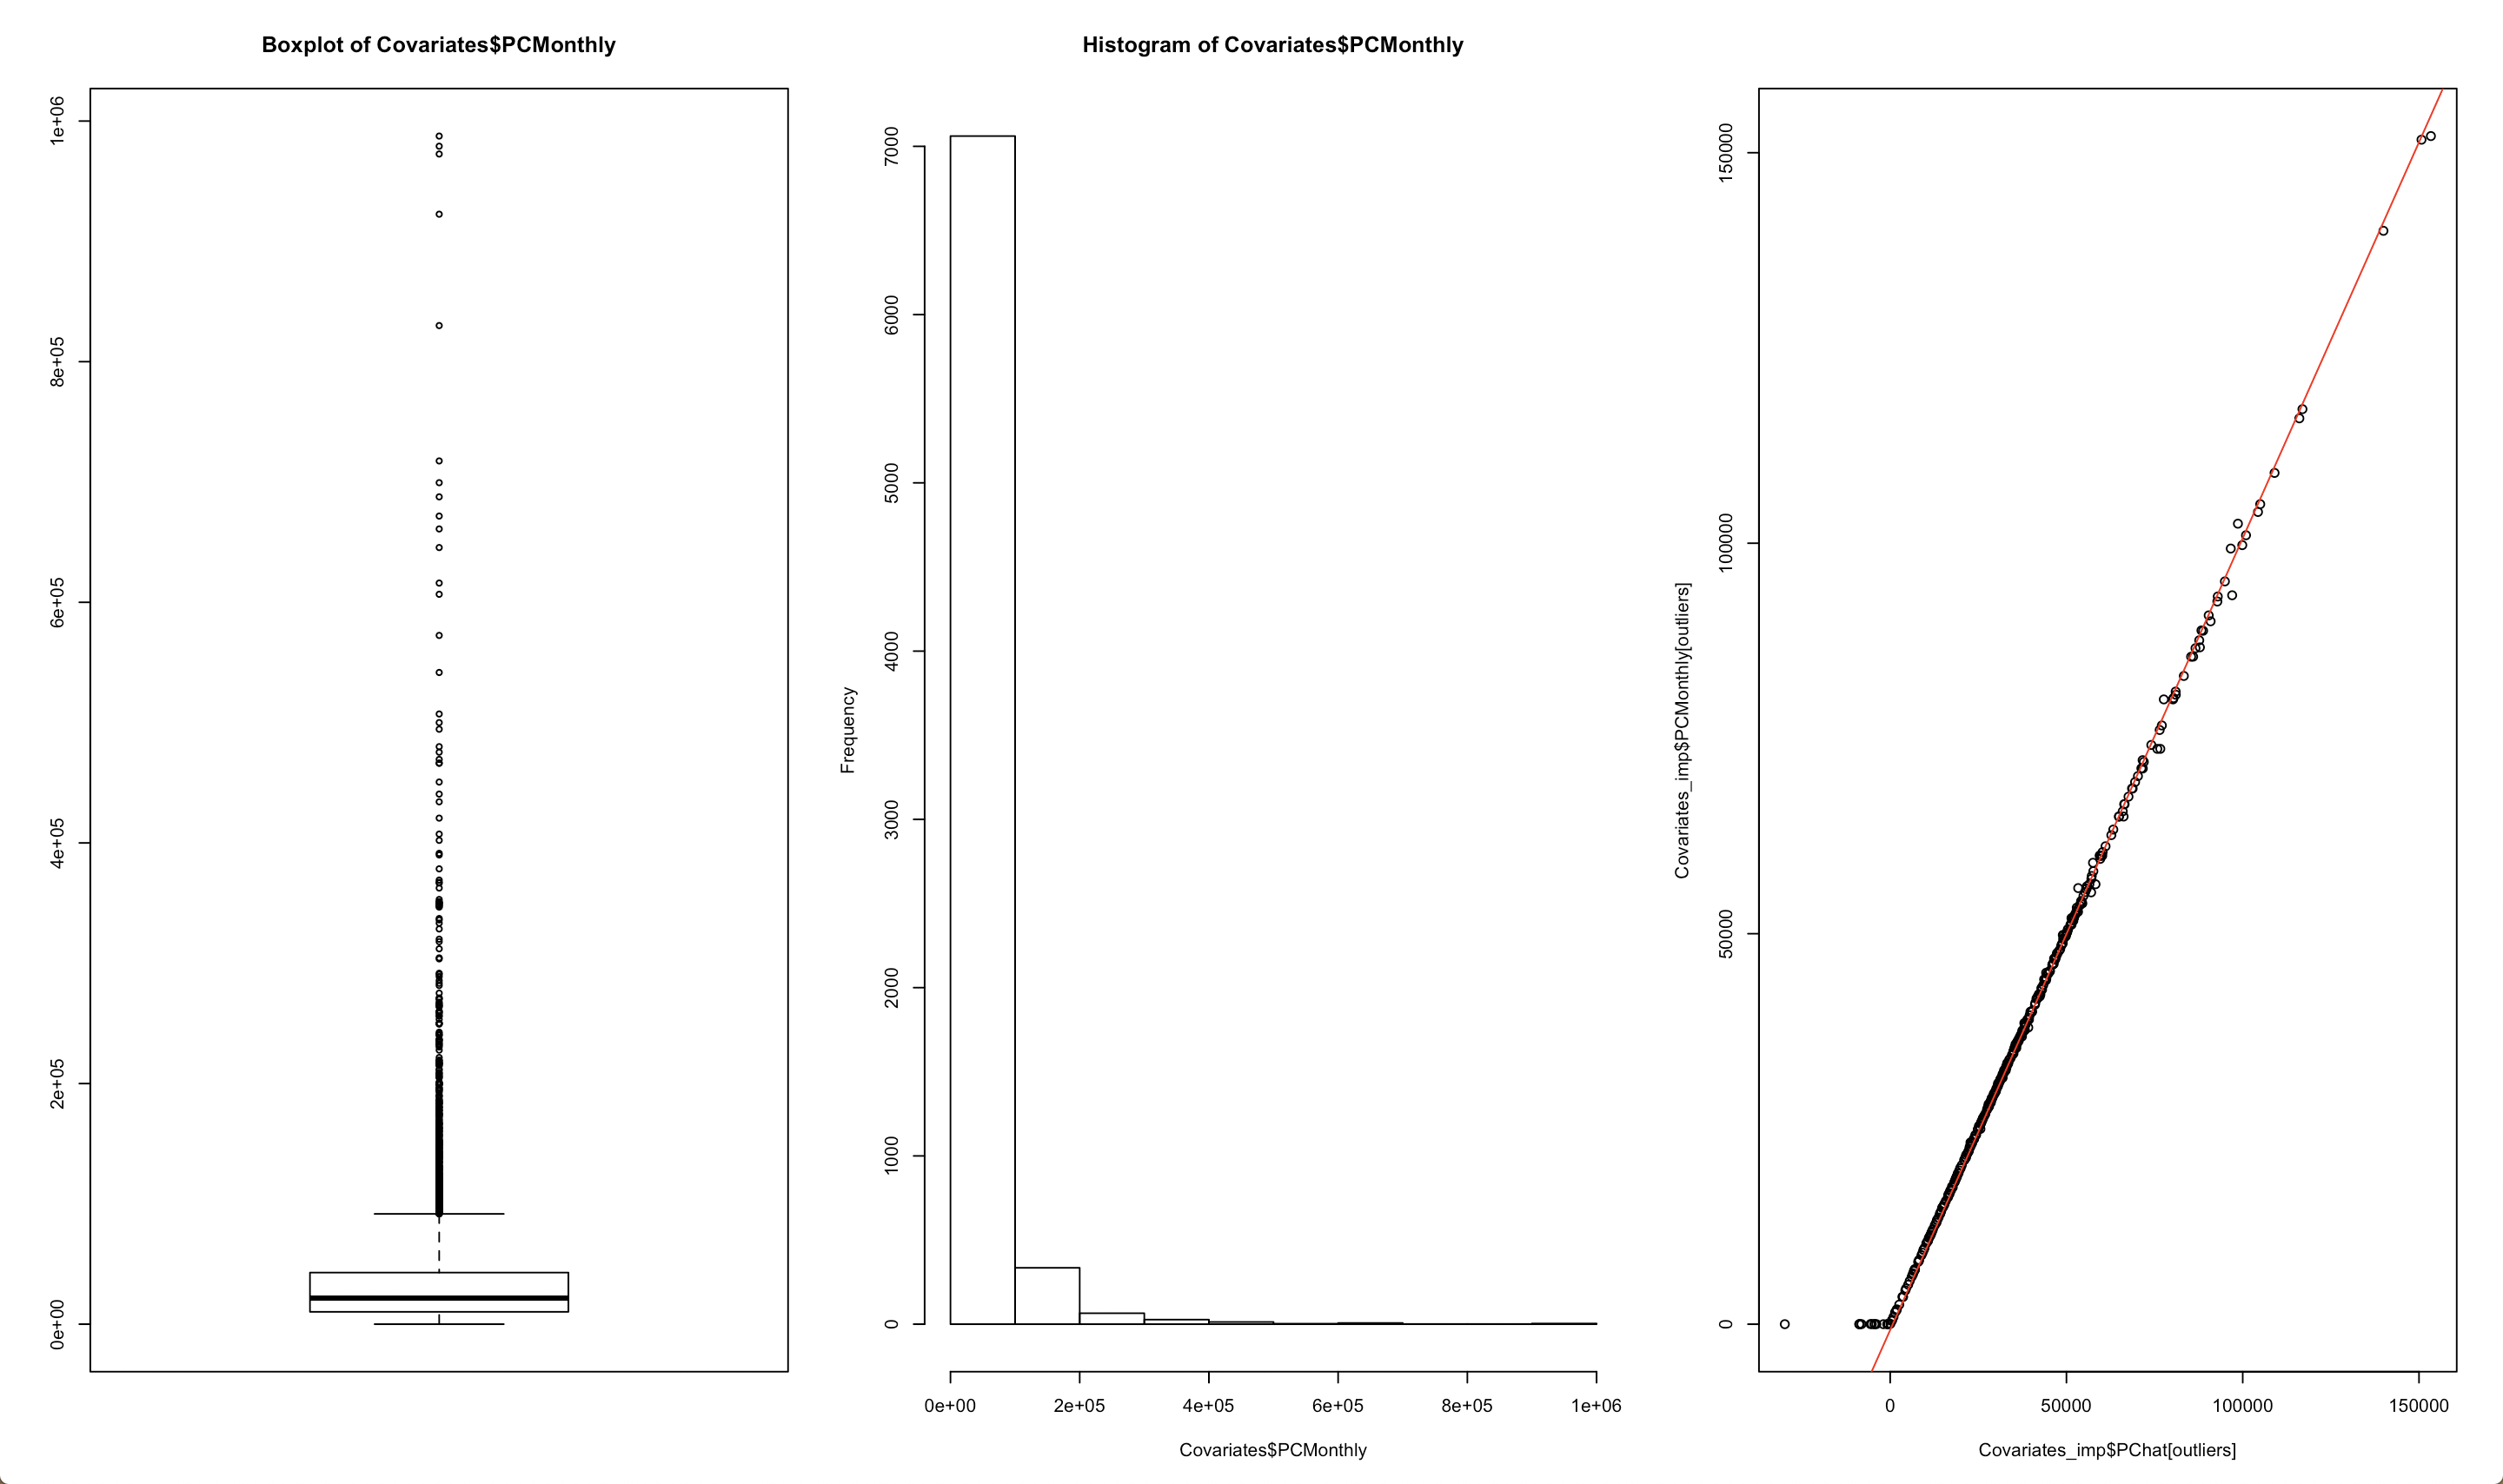
\includegraphics[width=\textwidth,height=5.20833in]{Pics/10.png}
\caption{\emph{Distribución de los ingresos (izquierda y centro) y Relación entre los valores predichos e imputados para los hogares con datos de ingresos faltantes (derecha).}}
\end{figure}

\hypertarget{imputacion-del-filtro}{%
\subsubsection*{Imputación del filtro}\label{imputacion-del-filtro}}
\addcontentsline{toc}{subsubsection}{Imputación del filtro}

El siguiente paso, luego de haber logrado imputar con éxito las covariables determinantes del gasto es precisamente utilizarlas para lograr imputar el gasto en bienes o servicios. Por lo general, las encuestas de ingresos y gastos preguntan si el hogar consumió o adquirió cierto bien o servicio específico. En caso de responder afirmativamente, se pregunta por la cantidad de dinero gastado en el bien o servicio y por la cantidad de artículos adquiridos en el periodo de referencia; en caso de responder negativamente, se procede a preguntar por el siguiente bien o servicio. Por supuesto, diferentes artículos tiene diferentes tasas de respuesta en sus filtros. De aquí en adelante, el valor a ser imputado en esta etapa es dicotóminco: sí o no. Si el valor imputado hubiera sido no, eso significaría que el hogar no debería tener ningún gasto asociado a ese ítem. Debido a la naturaleza del filtro, un modelo de regresión logística es conveniente para modelar la ausencia de respuesta en el filtro. De esta manera, la probabilidad de consumo (o compra)a un artículo \(i\) en particular es \(p_k = Pr(Filter_i = 1)\) y puede ser estimada por medio del siguiente modelo:

\[
\tilde{p}_k = logit^{-1}(\mathbf{x}_k \hat{\boldsymbol{\beta}}_i) =
\frac{exp(\mathbf{x}_k \hat{\boldsymbol{\beta}}_i)}{1+exp(\mathbf{x}_k \hat{\boldsymbol{\beta}}_i)}
\]

Las covariables incluidas en la matriz \(\mathbf{x}\) podrían ser las mismas utilizados para la imputación de los ingresos y, por supuesto, los ingresos en sí. Es decir, las covariables incluidas serían la composición del hogar, el estado ocupación y fuerza de trabajo de los miembros del hogar, la calidad de la vivienda, la ubicación del hogar y los ingresos del hogar. Asumiendo que los similares valores de \(\tilde p\) producirán valores de filtro similares, podemos ``pedir prestado'' un valor de filtro para imputar el que falta de un vecino con un valor similar de \(\tilde p\). Por lo tanto, el valor imputado del filtro para la unidad \(k\) es dada por

\[\hat{y}_k = y_{l(k)}\]

Donde \(l(k)\) es el ``elemento donante'', determinado por la minimización de una distancia simple entre los posibles donantes \(l\) a la unidad \(k\), dada por:

\[
D_{lk} = |\tilde p_k - p_l|
\]

Nótese que el donante \(l\) al elemento \(k\) es el elemento en el conjunto \(r_i\) con el valor más pequeño de la distancia \(D_{lk}\) entre todos los posibles \(l \in r_i\). Por regla general, todo los donantes deben estar en la misma provincia que la unidad con el valor faltante. Por ejemplo, considere el artículo arroz, para el cual algunos hogares no proveyeron ninguna respuesta asociada al filtro de compra. Como este es un artículo de consumo masivo en nuestra región, se supondría que la mayoría de hogares respondiera que efectivamente ha comprado arroz en el periodo de refernecia. De esta manera, al utilizar la regresión logística como modelo para la ausencia de respuesta del filtro del arroz, es posible encontrar que la distribución de las probabilidades estimadas de compra de arroz esté sesgada hacia el valor uno y alejada del valor cero, como lo muestra la siguiente figura. Está claro que la distribución de estas los valores imputados también debería estar cargada hacia el uno, reflejando la realidad de la compra de un artículo esencial como el arroz.

\begin{figure}
\centering
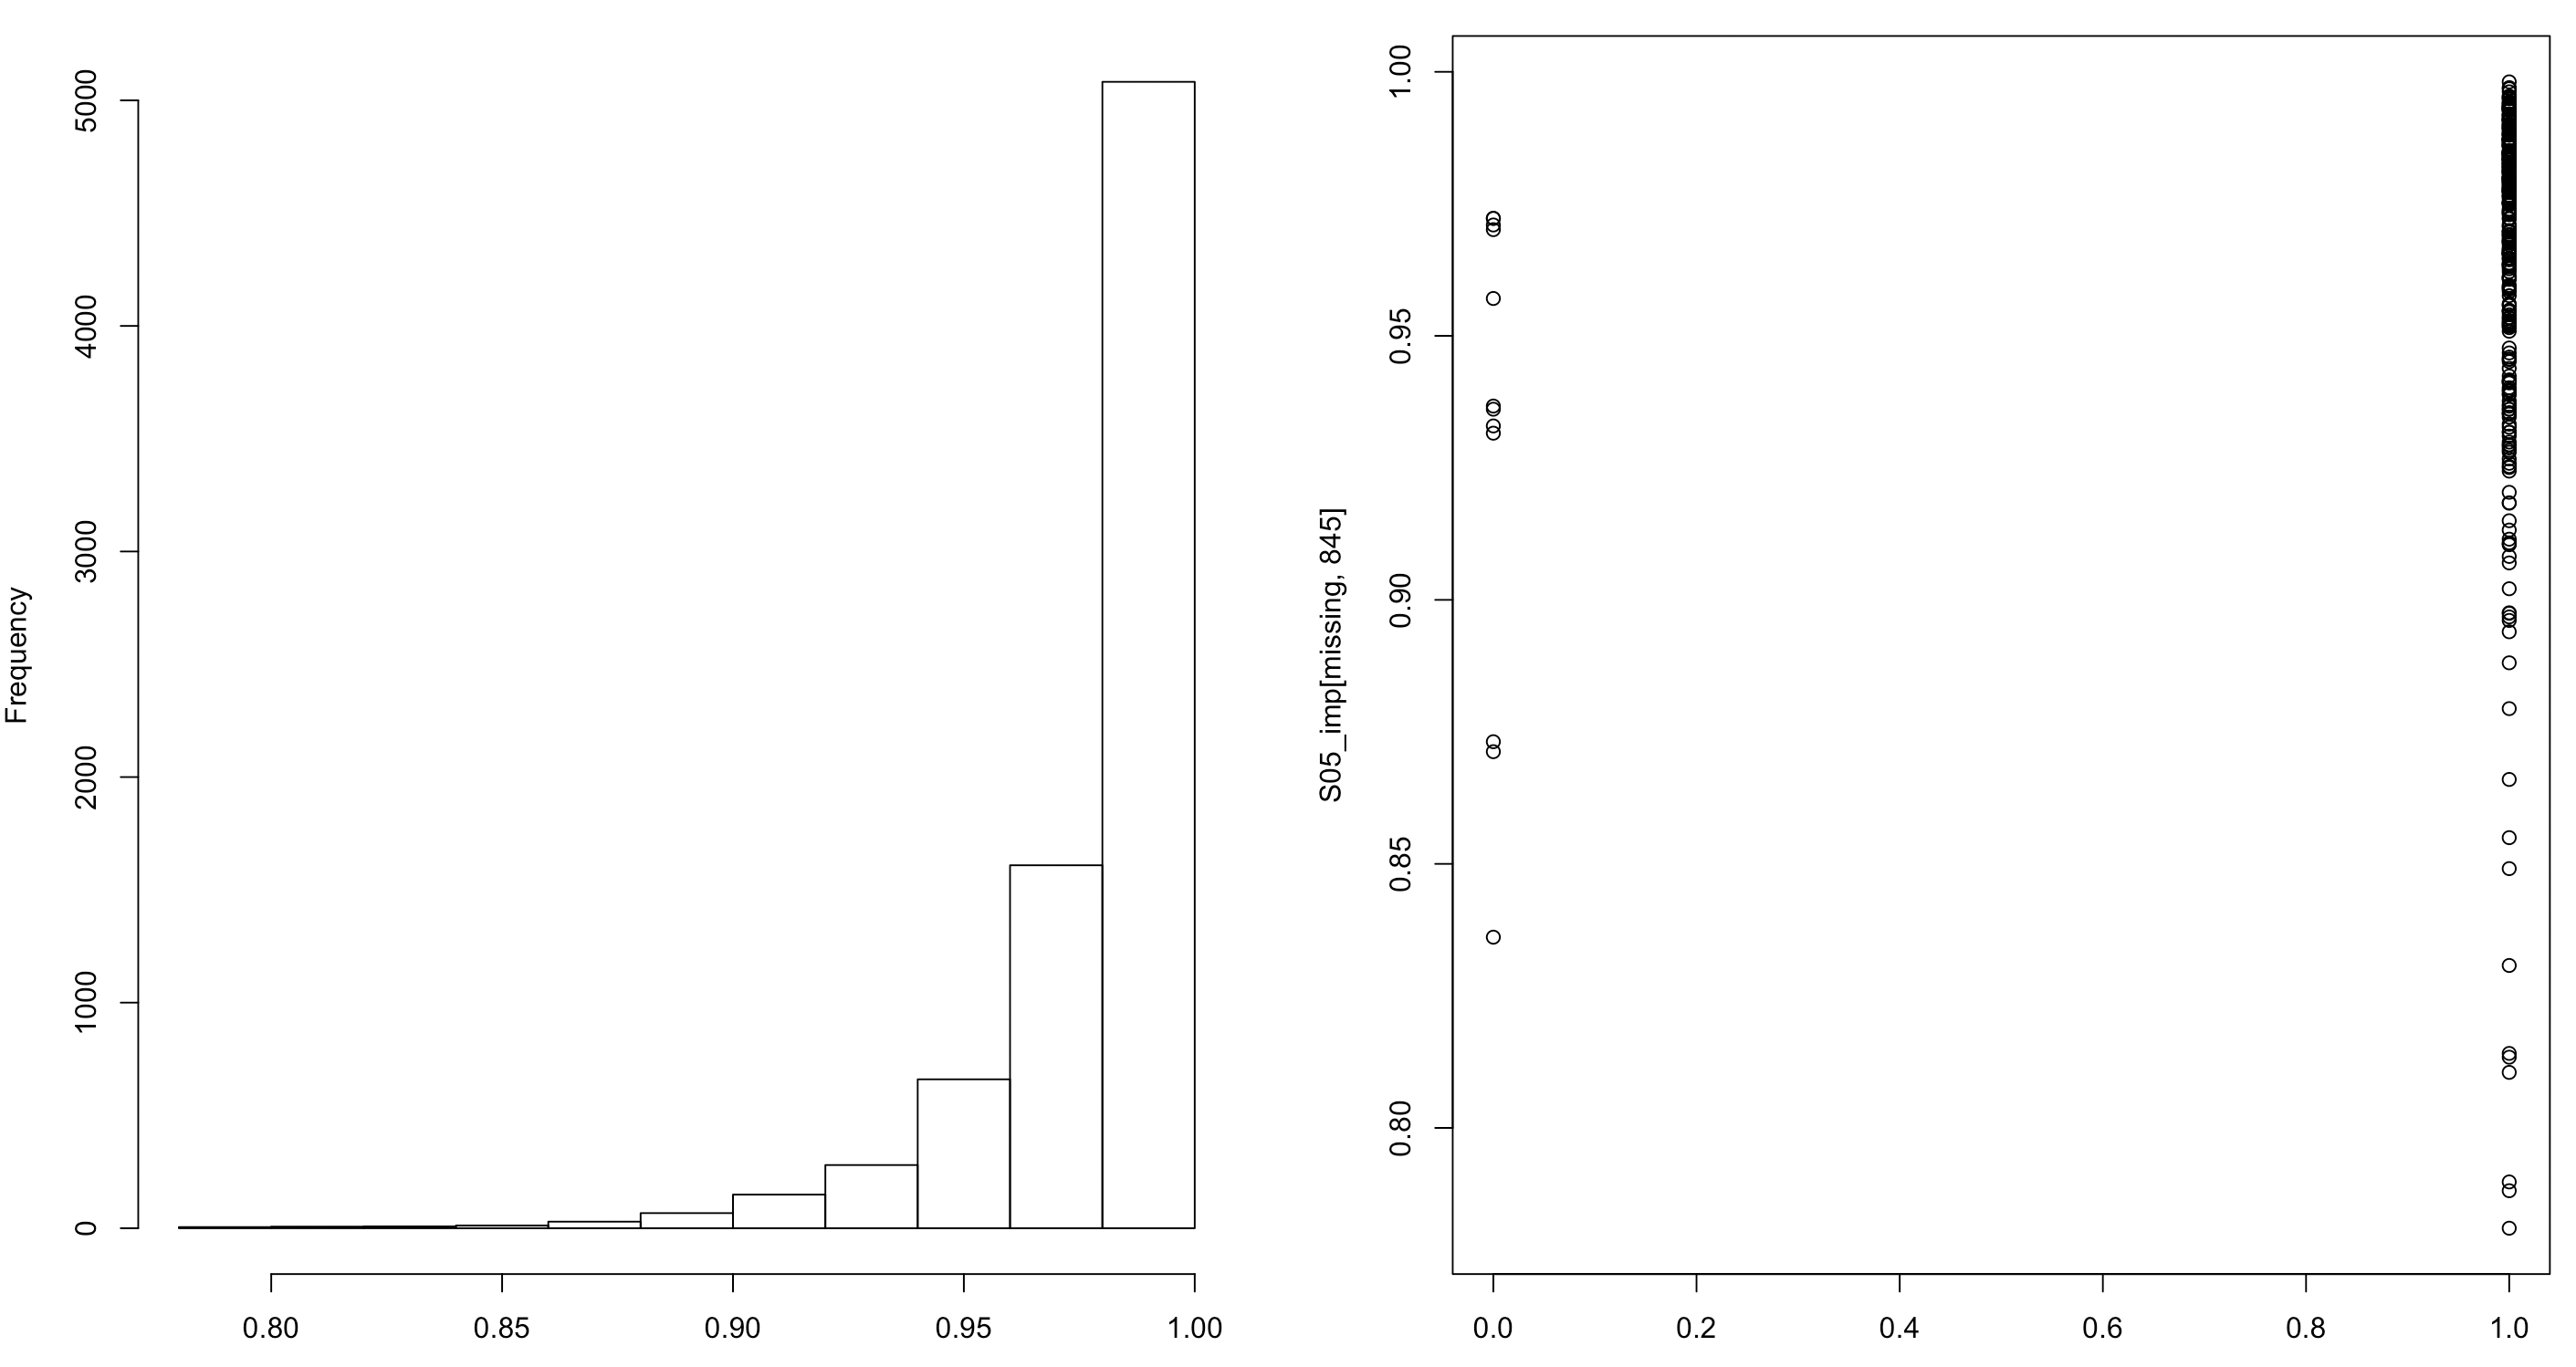
\includegraphics[width=\textwidth,height=5.20833in]{Pics/11.png}
\caption{\emph{Distribución de las probabilidades estimadas de compra de arroz (izquierda) y valores imputados para los hogares con valores faltantes en el filtro (derecha).}}
\end{figure}

Por otro lado, el filtro para algunos artículos de bajo consumo estará más sesgado hacia el valor cero. La siguiente figura muestra la distribución de las probabilidades estimadas de compra de un artículo de bajo consumo, así como los valores imputados.

\begin{figure}
\centering
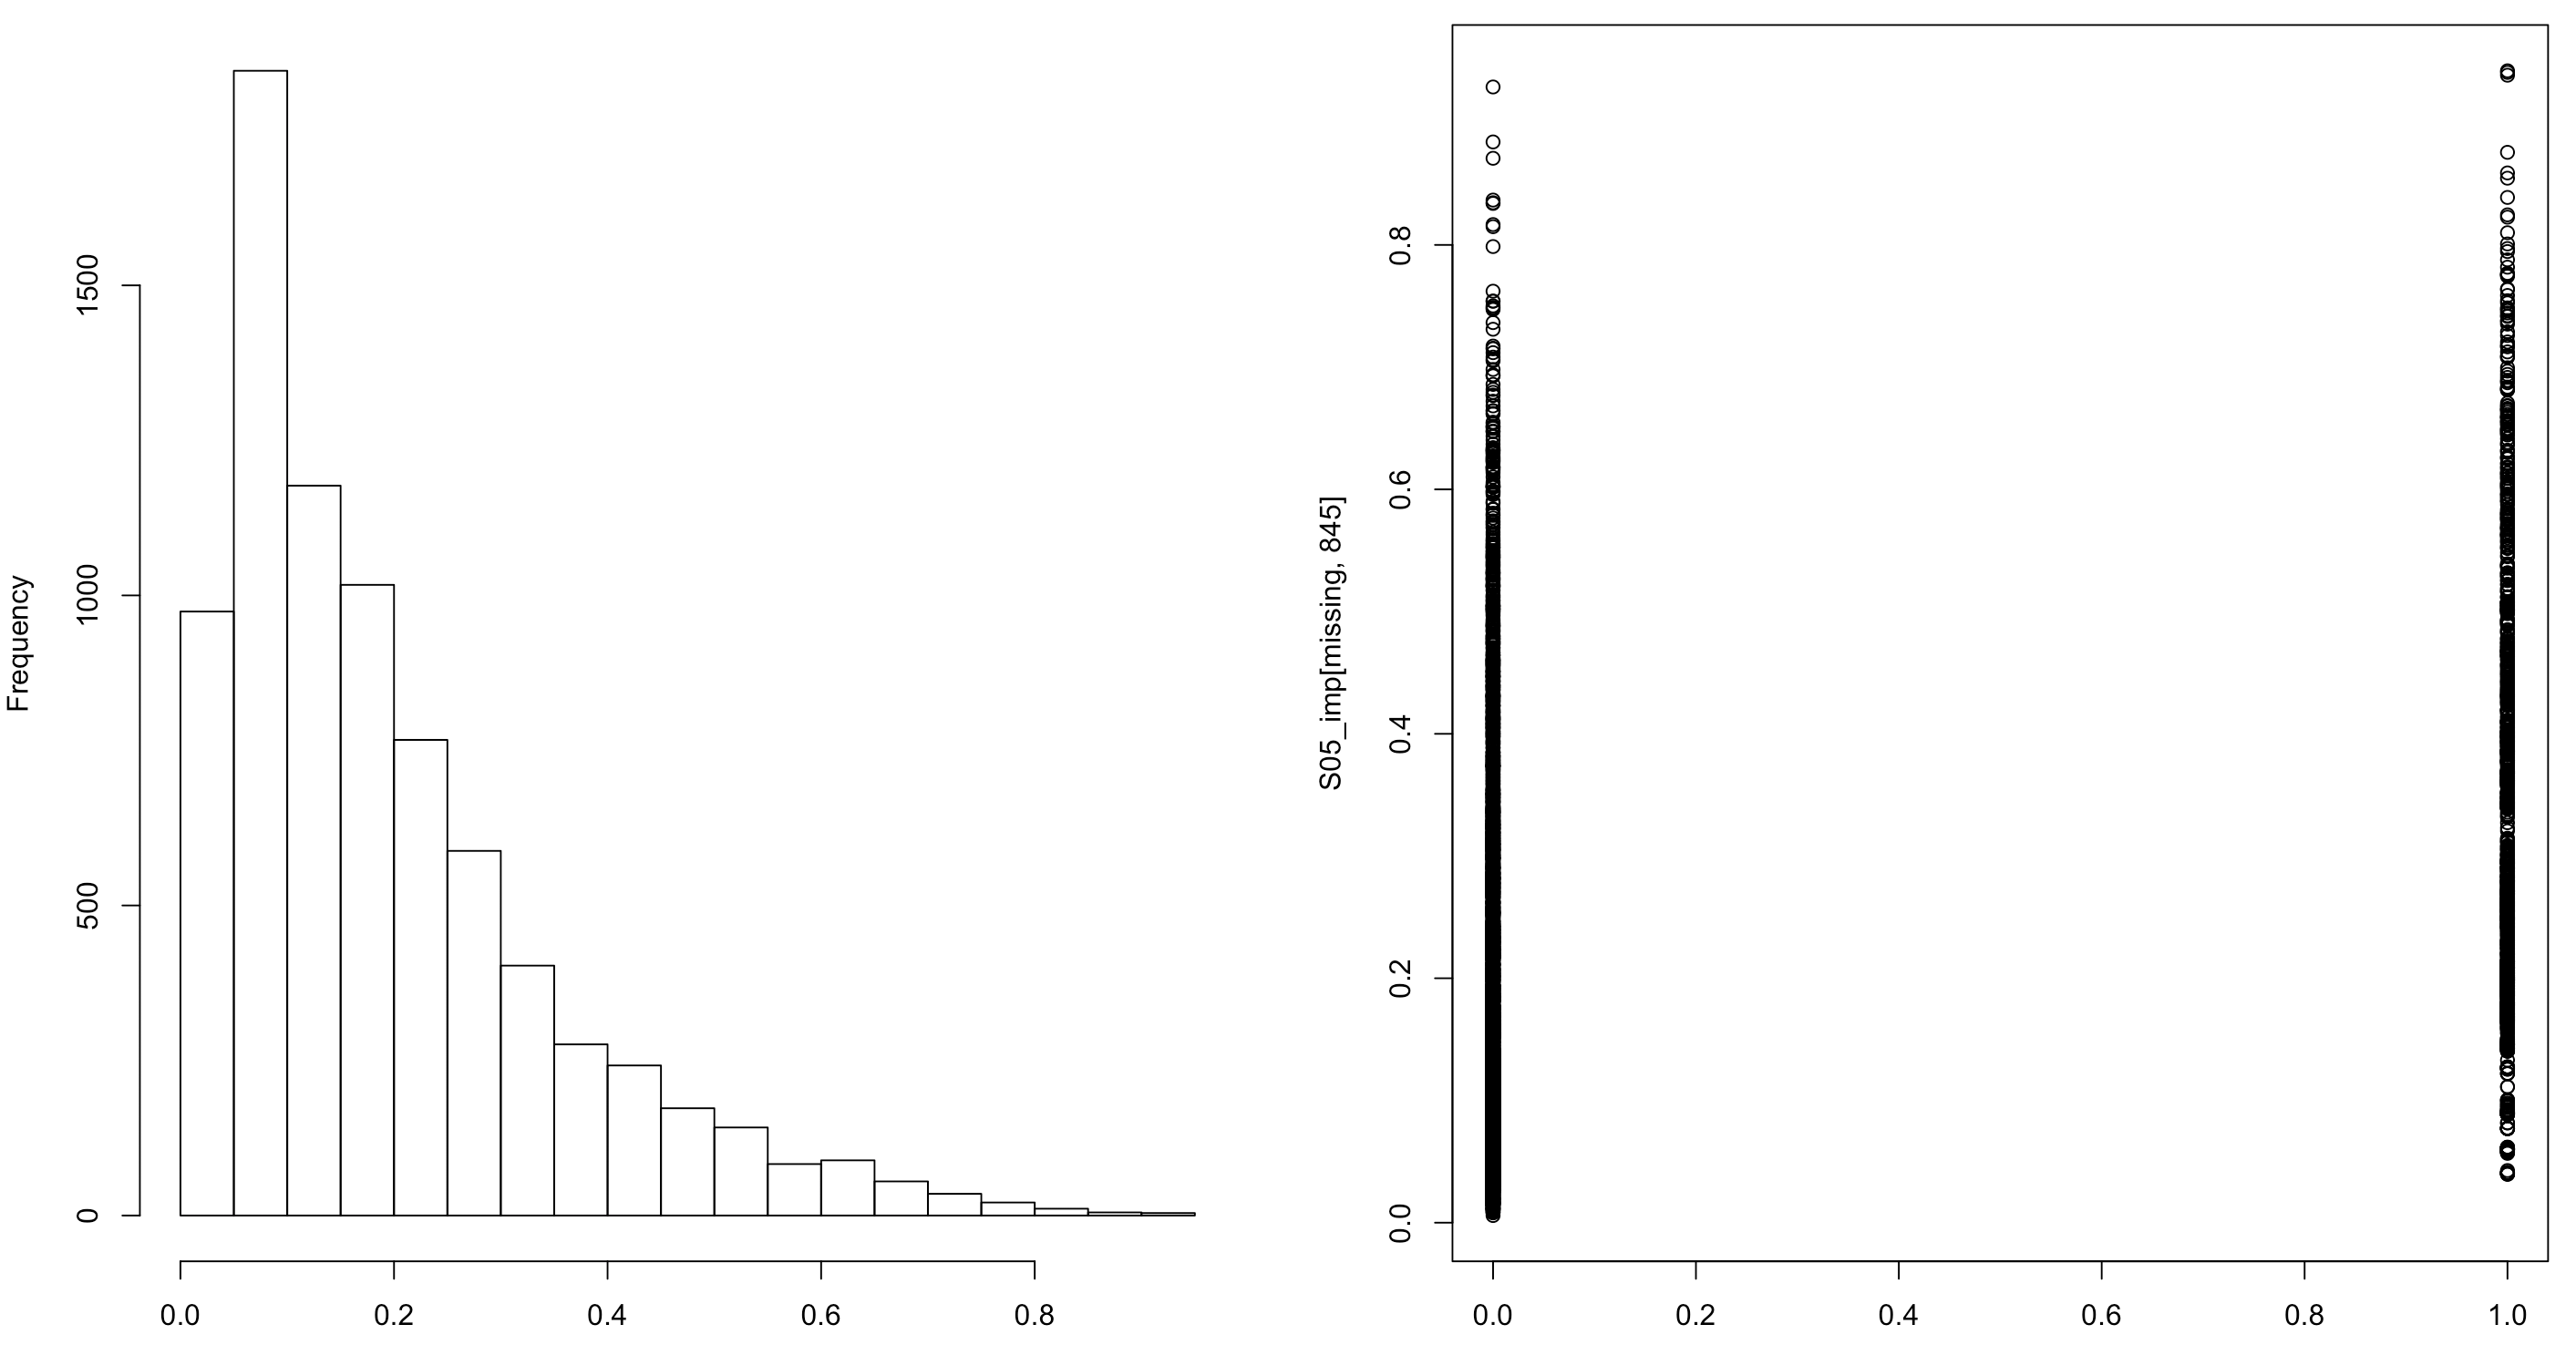
\includegraphics[width=\textwidth,height=5.20833in]{Pics/12.png}
\caption{\emph{Distribución de la probabilidad estimada de compra de un artículo de bajo consumo (izquierda) y sus valores imputados para los hogares que no respondieron el filtro (derecha).}}
\end{figure}

\hypertarget{imputacion-del-gasto}{%
\subsubsection*{Imputación del gasto}\label{imputacion-del-gasto}}
\addcontentsline{toc}{subsubsection}{Imputación del gasto}

Éste es el paso final del proceso de imputación y está fuertemente influenciado por los resultados de la imputación de la pregunta de filtro. En este paso, los hogares cuyo valor imputado de filtro es cero automáticamente tendrá un cero imputado como la cantidad de dinero gastado en ese artículo. Es decir, si el resultado de la imputación en el filtro es cero, esto implica directamente que el hogar no compró (o produjo) el artículo en el periodo de referencia, y por tanto la frecuencia de compra, la cantidad que ítems comprados y la cantidad de dinero gastado en ese artículo debe ser cero. Las unidades restantes deben tener un valor observado o imputado de uno en el filtro, y por lo tanto los valores faltantes del gasto deben ser imputados.

Observe que el grupo de donantes está restringido a los que tienen un valor de gasto distinto de cero en el artículo específico. Es decir, para aquellas unidades con un valor de filtro distinto de cero, un donante debe ser identificado. Para la imputación del gasto, la técnica del vecino más cercano con el método de regresión puede considerarse en el mismo sentido que fue implementado en la imputación de los ingresos. Por lo tanto, se considera un modelo lineal en donde las covariables incluidas en la matriz \(\mathbf{x}\) son la composición del hogar, el estado de ocupación y fuerza de trabajo, la calidad de la vivienda, la ubicación del hogar y los ingresos.

Volviendo a los ejemplos anteriores,la siguiente figura muestra la distribución de los gastos imputados sobre el arroz. Se nota que la cantidad de dinero gastado en este artículo es baja y que la relación entre los valores pronosticados del modelo y los valores imputados es fuertemente lineal.

\begin{figure}
\centering
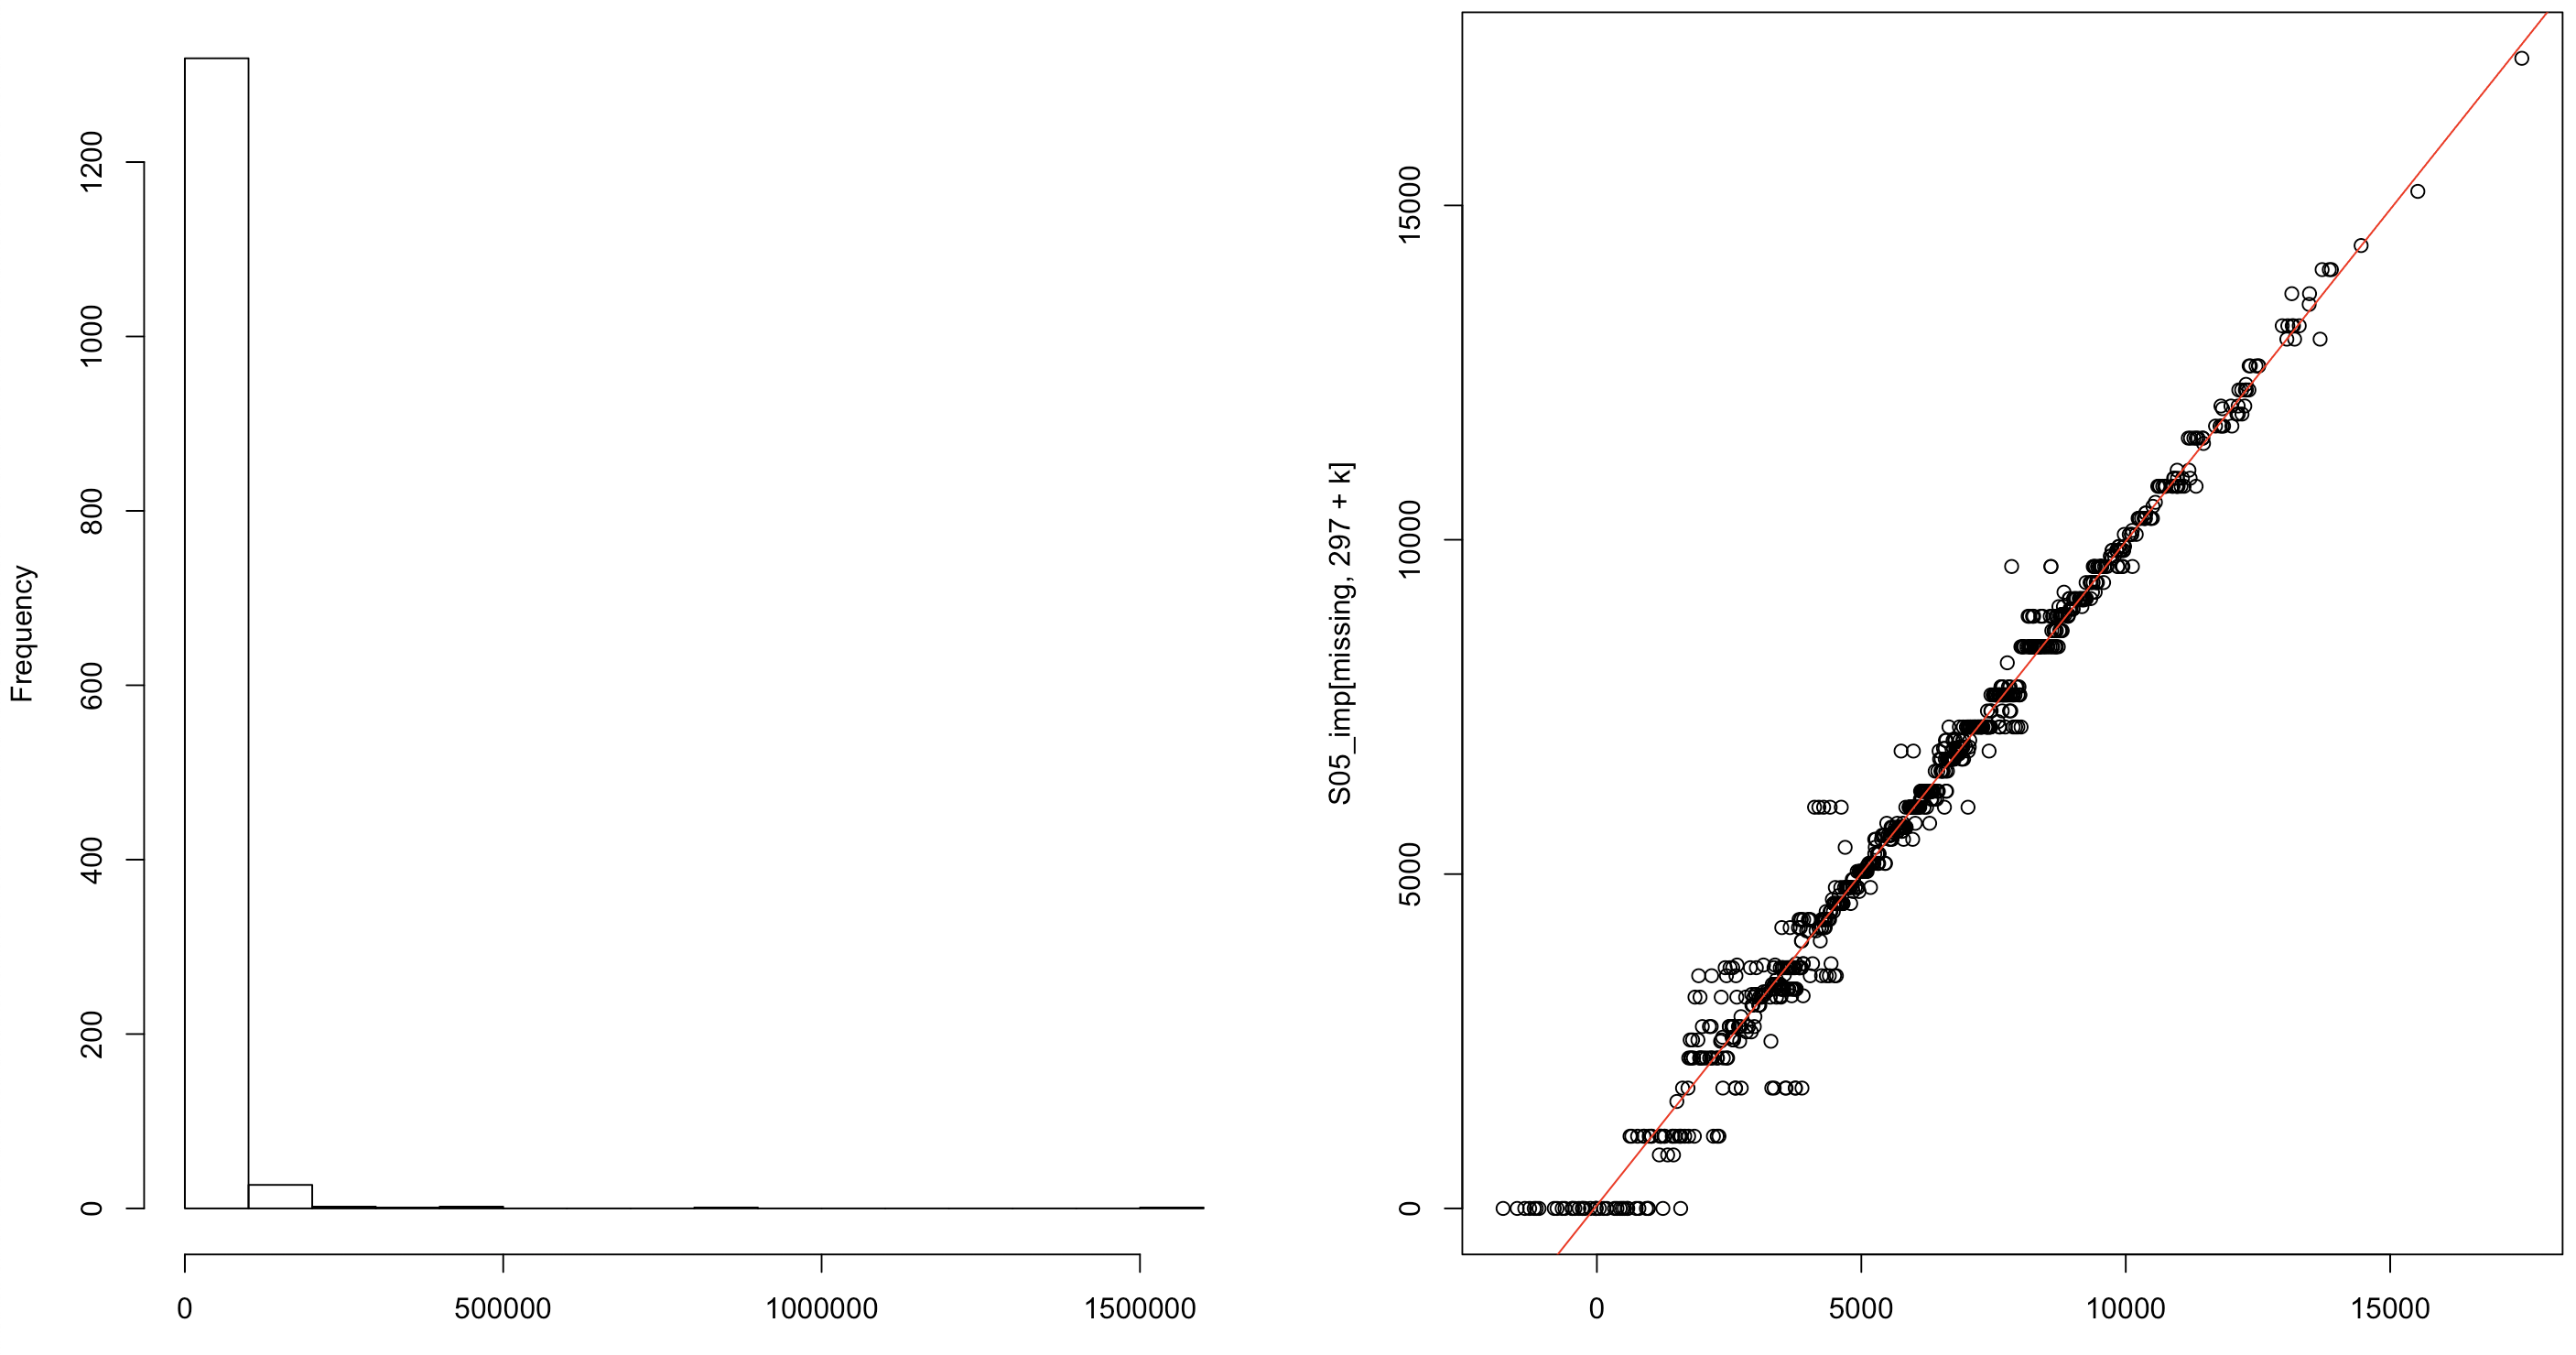
\includegraphics[width=\textwidth,height=5.20833in]{Pics/13.png}
\caption{\emph{Distribución de los gastos imputados sobre el arroz (izquierda) y relación entre los valores predichos e imputados para los hogares con valores faltantes en el gasto (derecha).}}
\end{figure}

\hypertarget{reponderacion-de-los-pesos-de-muestreo}{%
\section{Reponderación de los pesos de muestreo}\label{reponderacion-de-los-pesos-de-muestreo}}

Los procesos de inferencia estadistica establecidos en cualquier encuesta de hogares descansan sobre el principio de representatividad que afirma que es posible seleccionar una muestra y representar con bastante precisión y exactitud la realidad de la población de interés. A su vez, las propiedades estadísticas de la inferencia en encuestas de hogares descansan sobre las probabilidades de inclusión generadas por el diseño de muestreo que se implementó en la encuesta. En general el peso de muestreo \(w_k\) asociado a un individuo \(k\) en la muestra \(s\) es una función del inverso de la probabilidad de inclusión del individuo, así

\[
w_k \propto \frac{1}{Pr(k\in s)}
\]

Como se mencionó anteriormente, para conservar estabilidad en los pesos de muestreo, es posible definir diseños de muestreo auto-ponderados, en donde las unidades finales de muestreo tengan las misma probabilidad de inclusión, sin importar el tamaño de la unidad primaria de muestreo que la contiene. Este tipo de diseños es útil porque induce mayor control sobre las estimaciones finales. Es de notar que la conformación de los pesos de muestreo se transforma en un reto metodológico para el investigador, puesto que debe ajustarse a la realidad de la región en donde las poblaciones de los municipios se expanden cada vez más en el sector urbano y los marcos de muestreo de las áreas geográficas se desactualizan con rapidez. Varias soluciones a este problema han sido planteadas \autocite{Gambino_Silva_2009} y todas ellas requieren de esfuerzos económicos, logísticos y técnicos. Por ende, los equipos de los INE (a todo nivel) deben ser flexibles y adecuarse a esta realidad cambiante de la movilidad de las poblaciones, sobre todo en las áreas urbanas.

En condiciones ideales el marco de muestreo debería coincidir plenamente con la población finita. Sin emabargo, en general, no es posible contar con una lista de todos los elementos de la población y, en el contexto de las encuestas a hogares, no existe una lista que enumere todos los hogares de un país de manera actualizada, por lo que la práctica estándar es construir el marco de muestreo en varias etapas, seleccionando una muestra de áreas geográficas, realizando un empadronamiento exhaustivo de todos los hogares en las áreas seleccionadas y luego seleccionando hogares. Este esquema de muestreo hace que el marco de muestreo de las encuestas a hogares presente imperfecciones. El siguiente gráfico, adaptado de \textcite{Valliant_Dever_2017}, describe los problemas inferenciales que se deben surtir al trabajar con marcos de muestreo imperfectos y su relación con los pesos de muestreo originales.

XXXXXX incluir gráfico acá XXXXXXXXX

Para hacerle frente a las imperfeccciones del marco, la AsociacEl esquema de ponderación \emph{American Association for Public Opinion Research} (AAPOR) recomienda tratar la ausencia de respuesta de manera diferenciada y clasificar a cada unidad en la muestra en algunas de las siguientes categorías:

\begin{enumerate}
\def\labelenumi{\arabic{enumi}.}
\tightlist
\item
  ER (\emph{unidades elegibles que fueron respondientes efectivos}): casos elegibles para los cuales se ha recolectado una cantidad suficiente de información.
\item
  ENR (\emph{unidades eligibles no respondientes}): casos elegibles para los cuales no se recolectó ningún dato o la información fue parcialmente recolectada.
\item
  IN (\emph{unidades no elegibles}): casos de miembros no elegibles que no hacen parte de la población de interés.
\item
  UNK (\emph{unidades con elegibilidad desconocida}): casos en donde no se puede conocer si la unidad es elegible o no.
\end{enumerate}

Para construir los factores de expansión de una encuesta se recomienda seguir en este orden los siguientes procesos:

\begin{enumerate}
\def\labelenumi{\arabic{enumi}.}
\tightlist
\item
  Creación de los pesos básicos.
\item
  Descarte de las unidades no elegibles.
\item
  Ajuste por elegibilidad desconocida.
\item
  Ajuste por ausencia de respuesta.
\item
  Calibración por proyecciones poblacionales y variables auxiliares.
\item
  Preparación de la base de datos de respondientes.
\end{enumerate}

\hypertarget{creacion-de-los-pesos-basicos}{%
\subsubsection*{Creación de los pesos básicos}\label{creacion-de-los-pesos-basicos}}
\addcontentsline{toc}{subsubsection}{Creación de los pesos básicos}

Este primer paso ya ha sido explicado de forma detallada en la sección dedicada a la selección de la muestra. Observe que, asociado a cada esquema particular de muestreo, existe una única función que víncula a cada elemento con una probabilidad de inclusión en la muestra. De esta forma:

\[\pi_k = Pr (k \in s)\]

Por lo tanto, el primer paso, en la reponderación de los pesos de muestreo, es justamente la creación de los pesos básicos \(d_{1k}\) que se definen como el inverso multiplicativo de la probabilidad de inclusión

\[d_{1k} = \frac{1}{\pi_k}\]

Estos pesos son creados incluso para aquellas unidades que serán excluidas de la muestra porque son no elegibles o porque no proveyeron ninguna información y luego serán modificados convenientemente. La siguiente figura muestra la distribución típica de los pesos originales en una encuesta de hogares. A través de las modificaciones posteriores, esta distribución irá sufriendo algunos cambios. Si la distribución original de los pesos básicos difiere estructuralmente con la distribución final de los ponderadores, resultante de todos los ajustes debidos a las imperfecciones del marco, entonces las propiedades estadísticas de insesgamiento, consistencia y precisión podrían desvanecerse. Lo anterior implica que el nivel de desactaulización del marco de muestreo tiene implicaciones directas en la calidad de la inferencia. Por tanto, si el marco de meustreo es muy imperfecto, los ponderadores finales no inducirán una inferecnia precisa.

\begin{figure}
\centering
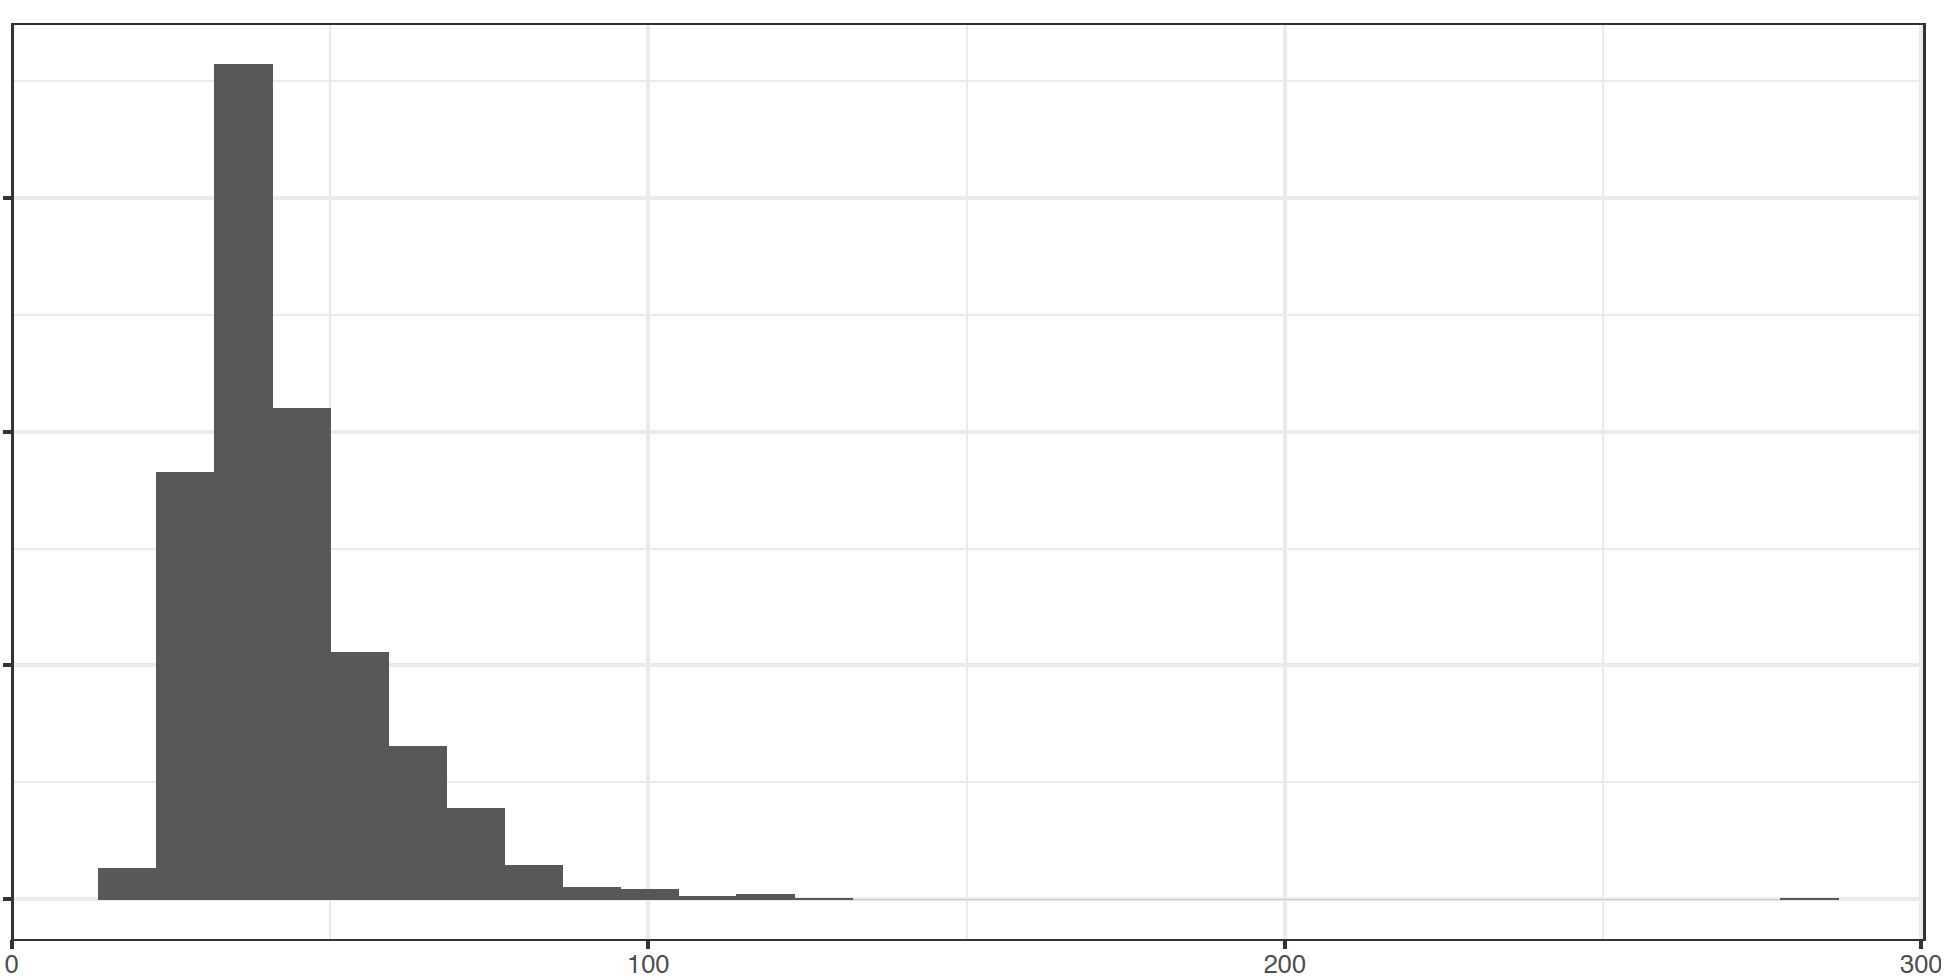
\includegraphics[width=\textwidth,height=5.20833in]{Pics/15.png}
\caption{\emph{Distribución de los pesos básicos de muestreo en una encuesta de hogares.}}
\end{figure}

\hypertarget{descarte-de-las-unidades-no-elegibles}{%
\subsubsection*{Descarte de las unidades no elegibles}\label{descarte-de-las-unidades-no-elegibles}}
\addcontentsline{toc}{subsubsection}{Descarte de las unidades no elegibles}

Si hay viviendas seleccionadas desde el marco de muestreo que han cambiado su estado de ocupación y ahora no contienen ningún hogar, entonces el segundo paso consiste en ajustar su peso básico de la siguiente manera:

\[
d_{2k} = 
\begin{cases}
0, \ \ \ \ \ \text{si la unidad $k$ no pertenece a la población objetivo}\\
d_{1k},\ \ \ \text{en otro caso }
\end{cases}
\]

\hypertarget{ajuste-por-elegibilidad-desconocida}{%
\subsubsection*{Ajuste por elegibilidad desconocida}\label{ajuste-por-elegibilidad-desconocida}}
\addcontentsline{toc}{subsubsection}{Ajuste por elegibilidad desconocida}

El tercer paso consiste en redistribuir el peso de las unidades cuyo estado de elegibilidad es desconocido. Por ejemplo, si la encuesta está enfocada en la población mayor de 15 años y hay personas que no proveen ninguna información acerca de su edad, entonces es necesario distribuir estos pesos. Esta situación también se puede presentar a nivel de hogar cuando no puede ser contactado porque nadie nunca atendió el llamado del encuestador (\emph{nadie en casa}). Se acostumbra a redistribuir los pesos de los UNK entre las unidades que sí disponen de su estatus de elegibilidad (ER, ENR, IN).

Luego, si no es posible determinar la elegibilidad de algunas unidades que aparecen en el marco de muestreo, se tendrá una muestra \(s\) que contendrá el conjunto de las unidades \emph{elegibles} en la muestra \(s_{e}\), el conjunto de las unidades \emph{no elegibles} en la muestra \(s_{n}\) y el conjunto de las unidades con \emph{elegibilidad desconocidad} \(s_{u}\). En este último caso, la elegibilidad de estos casos es desconocida, a no ser que de manera arbitraria sean clasificadas como ENR (elegibles no respondientes), o se tenga información auxiliar en el marco de muestreo que permita imputar su estado de elegibilidad.

Se recomienda formar \(B\) \((b = 1, \ldots, B)\) categorías\footnote{Se acostumbra a formar categorías con al menos 50 casos.} basadas en la información del marco de muestreo. Estas categorías pueden ser estratos o cruces de subpoblaciones. Siendo \(s_b\) la muestra de unidades en la categoría \(b\) (que incluye a ER, ENR y UNK), se define el factor de ajuste por elegibilidad como:

\[
a_b = \frac{\sum_{s_b}d_{2k}}{\sum_{s_b \cap s_e}d_{2k}}
\]
Para la categoría \(b\), los pesos ajustados por elegibilidad desconocida para aquellas unidades cuya elegibilidad si pudo ser establecida (independientemente de su estado de respuesta) estarán dados por la siguiente expresión:

\[
d_{3k} = a_b * d_{2k}
\]

\begin{figure}
\centering
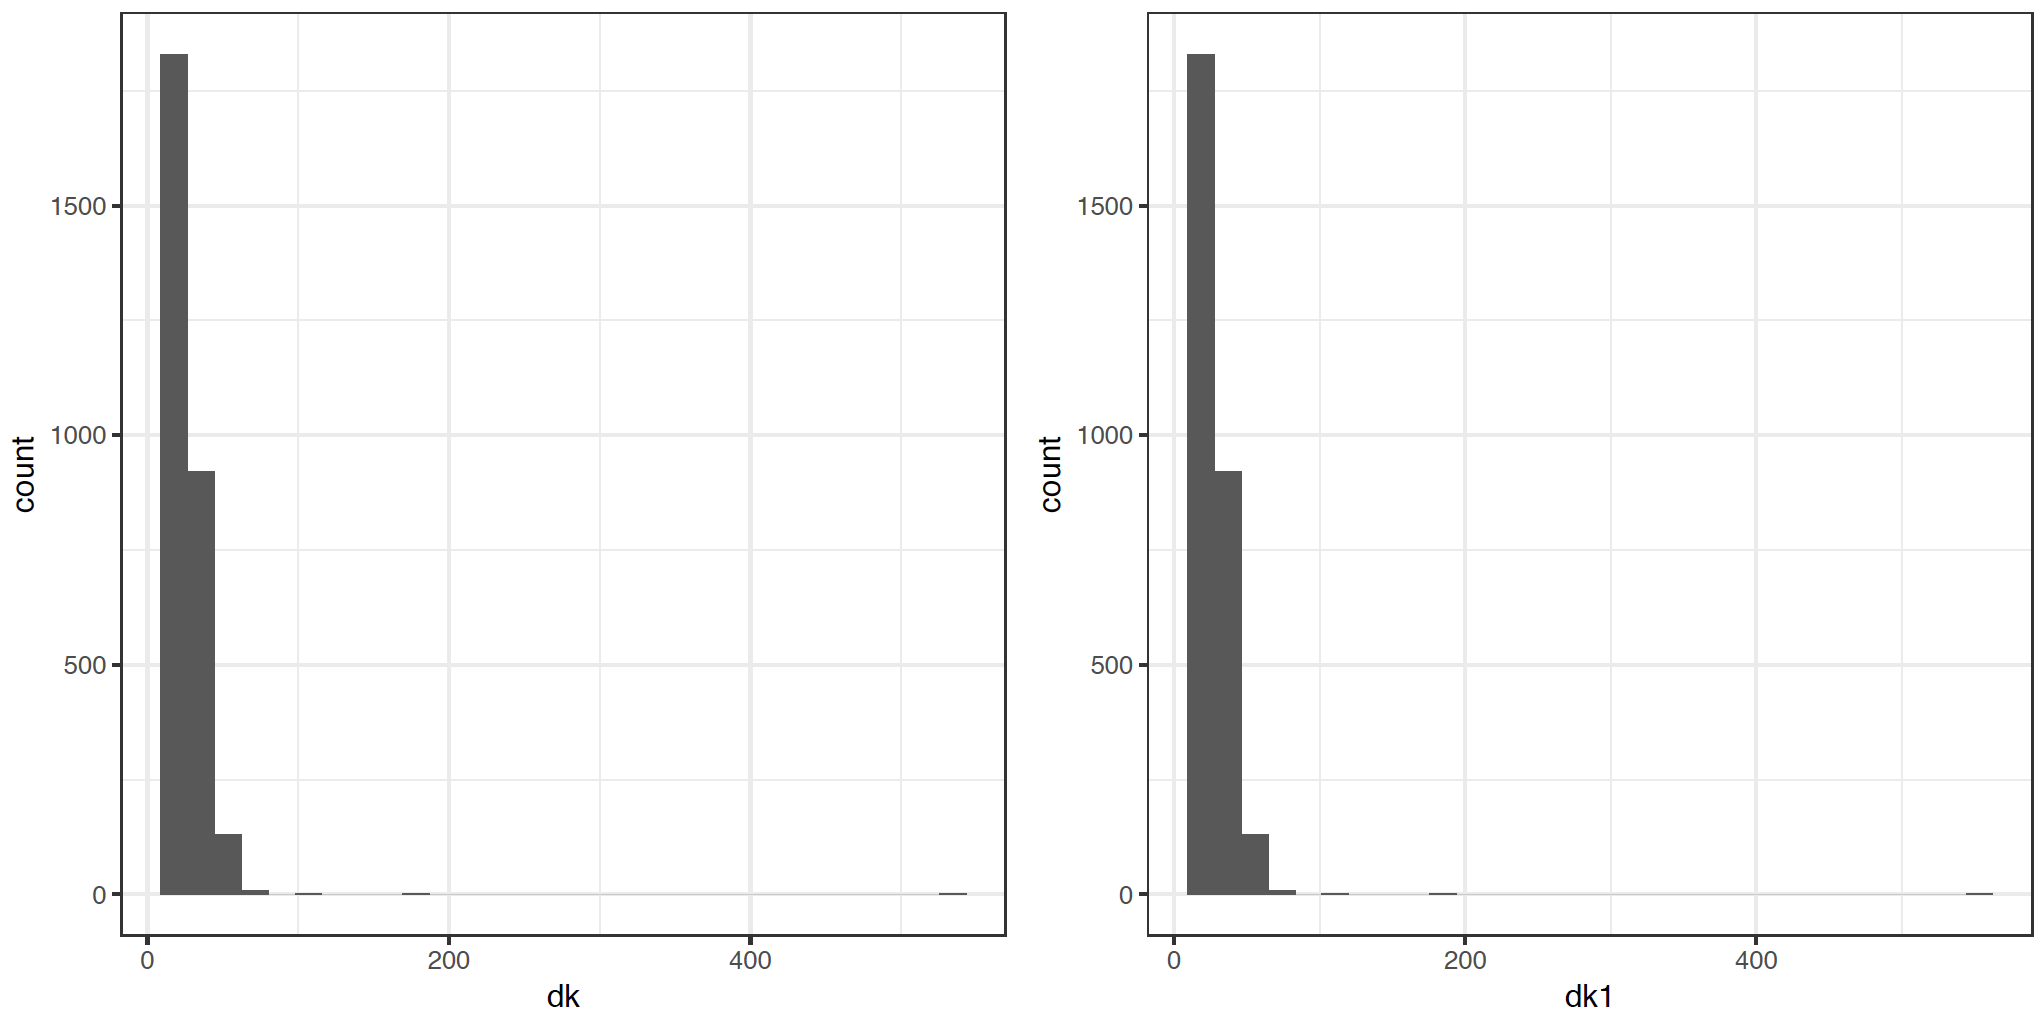
\includegraphics[width=\textwidth,height=5.20833in]{Pics/16.png}
\caption{\emph{Comparación de la distribución de los pesos básicos de muestreo (izquierda) con los pesos ajustados por el estado de elegibilidad (derecha) en una encuesta de hogares.}}
\end{figure}

\hypertarget{ajuste-por-ausencia-de-respuesta}{%
\subsubsection*{Ajuste por ausencia de respuesta}\label{ajuste-por-ausencia-de-respuesta}}
\addcontentsline{toc}{subsubsection}{Ajuste por ausencia de respuesta}

En este paso los pesos básicos de los ER se ajustan para tener en cuenta a los ENR. Al final del proceso, los pesos de los ER se incrementan para compensar el hecho de que algunas unidades elegibles no proveyeron información. Para el manejo efectivo de la ausencia de respuesta se consideran las siguientes variables aleatorias:

\[
I_k=
\begin{cases}
1,  &\text{si $k$ pertenece a la muestra $s$}\\
0,  &\text{en otro caso.}
\end{cases}
\]

\[
D_k=
\begin{cases}
1,  &\text{si $k$ pertenece al conjunto de respondientes $s_r$}\\
0,  &\text{en otro caso.}
\end{cases}
\]

Al suponer que la distribución de las respuestas puede ser estimada, entonces la probabilidad de respuesta (\emph{propensity score}) está dada por
\[
Pr(k\in s_r|k\in s)=Pr(D_k = 1|I_k = 1)=\phi_k 
\]

Si el patrón de ausencia de respuesta es completamente aleatorio (en donde la no respuesta no sigue ningún patrón específico) o aleatorio (en donde el patrón de la no respuesta puede ser explicado por covariables \(\mathbf{x}\) de la encuesta), entonces

\[
\phi_k = f(\mathbf{x}_k, \boldsymbol{\beta})
\]

Ahora, si es posible tener acceso a las covariables \(\mathbf{x}\), entonces es posible estimar el patrón de ausencia de respuesta mediante

\[
\hat{\phi}_k = f(\mathbf{x}_k, \hat{\boldsymbol{\beta}})
\]

Por otro lado, si el patrón de ausencia de respuesta es no aleatorio (en donde el patrón de la no respuesta es explicado por la variable de interés; por ejemplo cuando los desempleados son los que no responden), entonces

\[
\phi_k = f(\mathbf{y}_k, \beta)
\]

Luego, como no es posible tener acceso a la variables de interés para todos los individuos en la muestra (porque no todos respondieron), entonces no es posible estimar el patrón de ausencia de respuesta y por ende hay sesgo. Bajo los dos primeros escenarios, es posible definir el siguiente estimador insesgado
\[
\hat{t}_y=\sum_{k\in s_r}d_{4k}y_k
\]

En donde

\[
d_{4k} = \frac{d_{3k}}{\hat{\phi_k}}
\]

Nótese que el sesgo se anula puesto que

\[
E(I_kD_k) 
= EE(I_kD_k|I_k) 
= E(I_k)E(D_k|I_k) = \pi_k \phi_k
\]

XXXXXXXX

Si se tiene acceso a información auxiliar (contenida en el marco de muestreo o en otras preguntas de la encuesta), y si se considera que el mecanismo que genera la ausencia de respuesta en la encuesta de hogares es MAR, es posible ajustar un modelo para la ausencia de respuesta (en donde la variable dependiente es una variable indicadora de la respuesta del individuo por lo general supeditado a una distribución Bernoulli o Binomial). \textcite{Kim_Riddles_2012} muestran que es posible utilizar un modelo basado en el \emph{propensity score} de las respuestas. Si la muestra de los respondientes se denota como \(s_r\) entonces la probabilidad de que un individuo conteste es \(\phi_k = Pr(k \in s_r)\). Al suponer que existe un vector de información auxiliar \(\mathbf{z}_k\) conocido para todo \(k\in s\) es posible estimarla por medio de un modelo de regresión logística; esto es,

\[
\hat{\phi}_k = \frac{\exp\{\mathbf{z}_k'\hat{\boldsymbol{\beta}}\}}{1 + \exp\{\mathbf{z}_k'\hat{\boldsymbol{\beta}}\}}
\]

donde \(\hat{\mathbf{\beta}}\) es el vector de coeficientes estimado de la regresión logística. Finalmente, el nuevo peso estimador para un total poblacional, con el ajuste debido a la ausencia de respuesta no ignorable, queda expresado como

\[
\hat{t}_{y}^{(adj)}= \sum_{k\in s_r} \frac{w_k}{\hat{\phi}_k}y_k
\]

XXXXXX

\begin{figure}
\centering
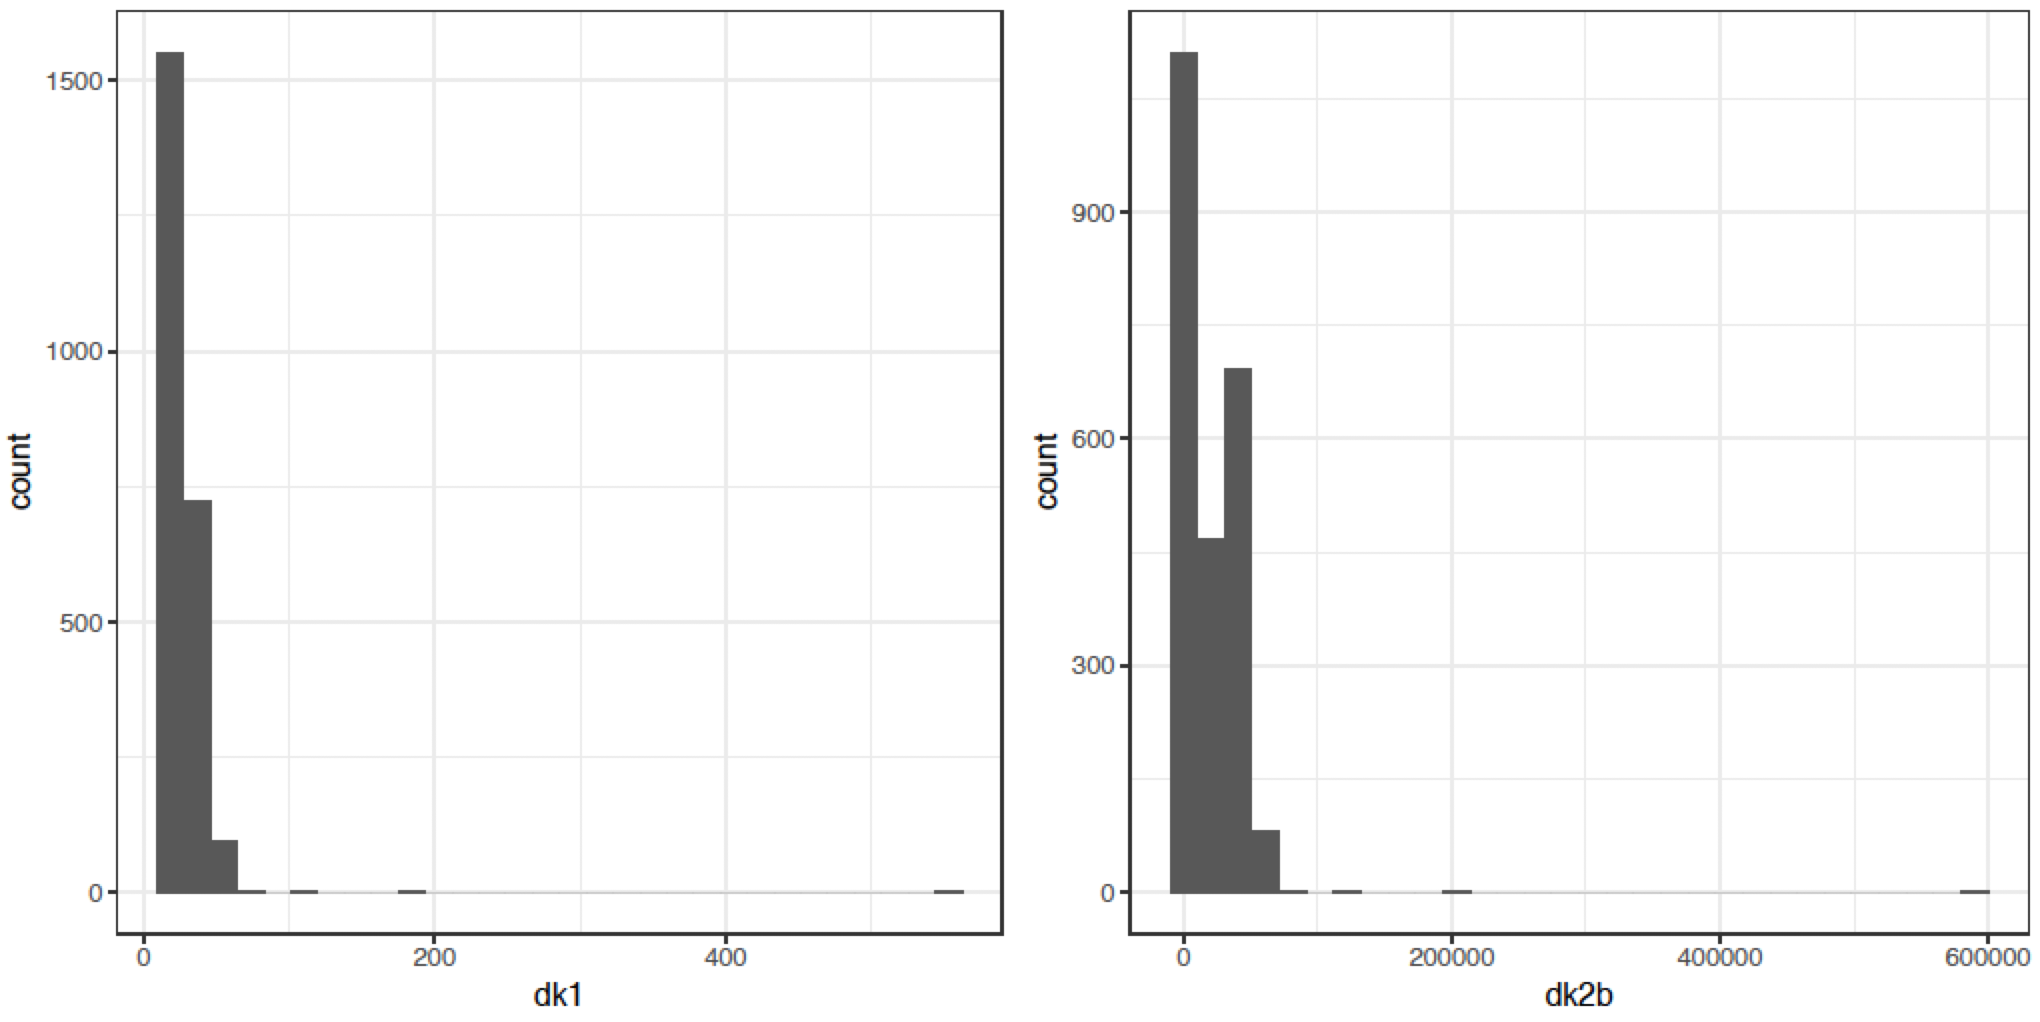
\includegraphics[width=\textwidth,height=5.20833in]{Pics/17.png}
\caption{\emph{Comparación de la distribución de los pesos básicos de muestreo (izquierda) con los pesos ajustados por ausencia de respuesta (derecha) en una encuesta de hogares.}}
\end{figure}

\hypertarget{calibracion-de-los-pesos}{%
\subsubsection*{Calibración de los pesos}\label{calibracion-de-los-pesos}}
\addcontentsline{toc}{subsubsection}{Calibración de los pesos}

Después de conformar el sistema de ponderación de pesos de muestreo en la encuesta, es posible calibrar estos pesos con la información auxiliar disponible para cada país, a nivel nacional, por estratos de interés, e incluso por variable continuas sobre las que se tenga interés. \textcite{Sarndal_Lundstrom_2006} afirman que cuando los estudios por muestreo están afectados por la ausencia de respuesta, es deseable tener las siguientes propiedades en la estructura inferencial que sustenta el muestreo:

\begin{enumerate}
\def\labelenumi{\arabic{enumi}.}
\tightlist
\item
  Sesgo pequeño o nulo.
\item
  Errores estándares pequeños.
\item
  Un sistema de ponderación que reproduzca la información auxiliar disponible\footnote{Por ejemplo, el número de hogares o habitantes en el país.}.
\item
  Un sistema de ponderación que sea eficiente al momento de estimar cualquier característica de interés en un estudio multipropósito.
\end{enumerate}

A pesar de que cada vez es más extendido el uso de los pesos calibrados en las encuestas de América Latina, es necesario que se disemine más esta práctica metodológica que induce estimadores muestrales que reproducen exactamente la información auxiliar conocida a nivel poblacional. Debido a la construcción teórica de los estimadores de calibración, los pesos finales responden a la siguiente restricción

\[
\sum_{s}w^*_{k}\boldsymbol{x}_k = \sum_{U}\boldsymbol{x}_{k} = \boldsymbol{t}_{\boldsymbol{x}}
\]

El ejemplo más básico se encuentra cuando se desea que los pesos de muestreo deberían reproducir con exactitud el tamaño de las regiones \(N_h\) y el tamaño del país \(N\). Es así como, utilizar la metodología de calibración \autocite{Deville_Sarndal_1992} hace que se cumpla la siguiente ecuación de calibración sobre los nuevos pesos calibrados \(w_k^*\) para todos lo estratos explícitos

\[
\sum_{s_h} w_k^* = N_h
\]

Esta coherencia entre las cifras oficiales y las que la encuesta puede producir hace que sea preferible el uso de los estimadores de calibración. Las anteriores características son satisfechas al usar el enfoque de calibración que induce una estructura inferencial robusta en presencia de información disponible puesto que reduce tanto el error de muestreo como el error debido a la ausencia de respuesta. Los estimadores de calibración son \textbf{aproximandamente insesgados}, pero la magnitud del sesgo está dada por la siguiente expresión:

\[
Bias(\hat{t}_{y, cal}) = E_p \left[ \sum_{k \in s} (w_k - d_k) y_k \right]
\]

Si los nuevos pesos calibrados son cercanos a los pesos originales en todas las posibles muestras, entonces el sesgo será insignificante. Ahora, si el tamaño de muestra es insuficiente no conviene utilizar este tipo de estimadores. Además, se sugiere que el coeficiente de variación del estimador de Horvitz-Thompson para las covariables (inducidas por todos los cruces y celdas considerados) sea menor del 10\% para asegurar que el sesgo de los estimadores de calibración sea despreciable.

Por otro lado, cuando se tienen múltiples variables discretas es posible que el cruce de categorías contenga muy pocas unidades para las cuales se deba ajustar los pesos originales. Esto induce sesgo en cada subgrupo ajustado. Si aún así se decide optar por múltiples aumentar las variables de calibración, es necesario hacer un chequeo empírico del ajuste que cada modelo pueda tener con todas las variables de la encuesta, aunque se advierte que este chequeo a veces puede ser demorado e ir en contravía de las apretadas agendas de producción estadísticas que se manejan en el INE.

\textcite{Silva_2004} presenta algunas consideraciones al respecto del sesgo que puede generarse al usar esta metodología en las encuestas de hogares y aborda algunos criterios para evaluar la calidad de la calibración.

La idea general del proceso de calibración es encontrar un número de restricciones parsimonioso que permita tener estimaciones aproximadamente insesgadas con una varianza menor a la generada con los factores de expansión originales. En general los INE podrán clasificar sus procesos de calibración en una de las siguientes tres categorías:

\begin{enumerate}
\def\labelenumi{\arabic{enumi}.}
\tightlist
\item
  Calibración con variables continuas, que es el caso en donde la calibración se realiza con los totales de variables continuas como ingreso, gasto, entre otras.
\item
  Post-estratificación con variables categóricas, que representa el caso en donde la calibración se realiza con los tamaños poblacionales (basados en proyecciones demográficas o registros administrativos) de subgrupos de interés.
\item
  \emph{Raking} con variables categóricas, que se define como una calibración sobre los tamaños marginales de tablas de contingencia de subgrupos de interés. A diferencia del caso anterior, esta calibración no tiene en cuenta los tamaños de los cruces, sino solo los tamaños marginales; por ende, este método induce menos restricciones.
\end{enumerate}

En un encuesta de hogares las restricciones de calibración pueden establecerse sobre características de hogares y características de personas al mismo tiempo. De esta forma, por ejemplo, es posible calibrar sobre las proyecciones demográficas de personas y al mismo tiempo controlar las estimaciones del número de hogares en el país de manera conjunta. \textcite{Estevao_Sarndal_2006} discuten una amplia variedad de casos en donde se calibra conjuntamente en distintos niveles de desagregación sobre diferentes esquema de muestreo. Por ejemplo, para la \emph{Encuesta Continua de Empleo} de Bolivia la calibración está inducida por una post-estratificación sobre los tamaños poblacionales de los cruces resultantes entre las variable Departamento (hay 9 departamentos), Zona (rural y urbano) y PET (con dos categorías: mayor o igual a 10 años y menor de 10 años).

El asesor regional dio una charla acerca de la metodología de calibración al equipo del Departamento de Investigación y Desarrollo, en donde se presentaron algunas medidas de calidad como protección en contra del sesgo generado por considerar demasiadas restricciones y se resaltó la importancia de que las variables utilizadas para la calibración sean estimadas de manera precisa por los estimadores clásicos de muestreo. Por ejemplo, si el número de personas por hogar es utilizada como una variable de calibración (utilizando como total auxiliar las proyecciones demográficas), entonces el coeficiente de variación del estimador de Horvitz-Thompson sobre esta variable debería ser menor al 10\%.

\begin{figure}
\centering
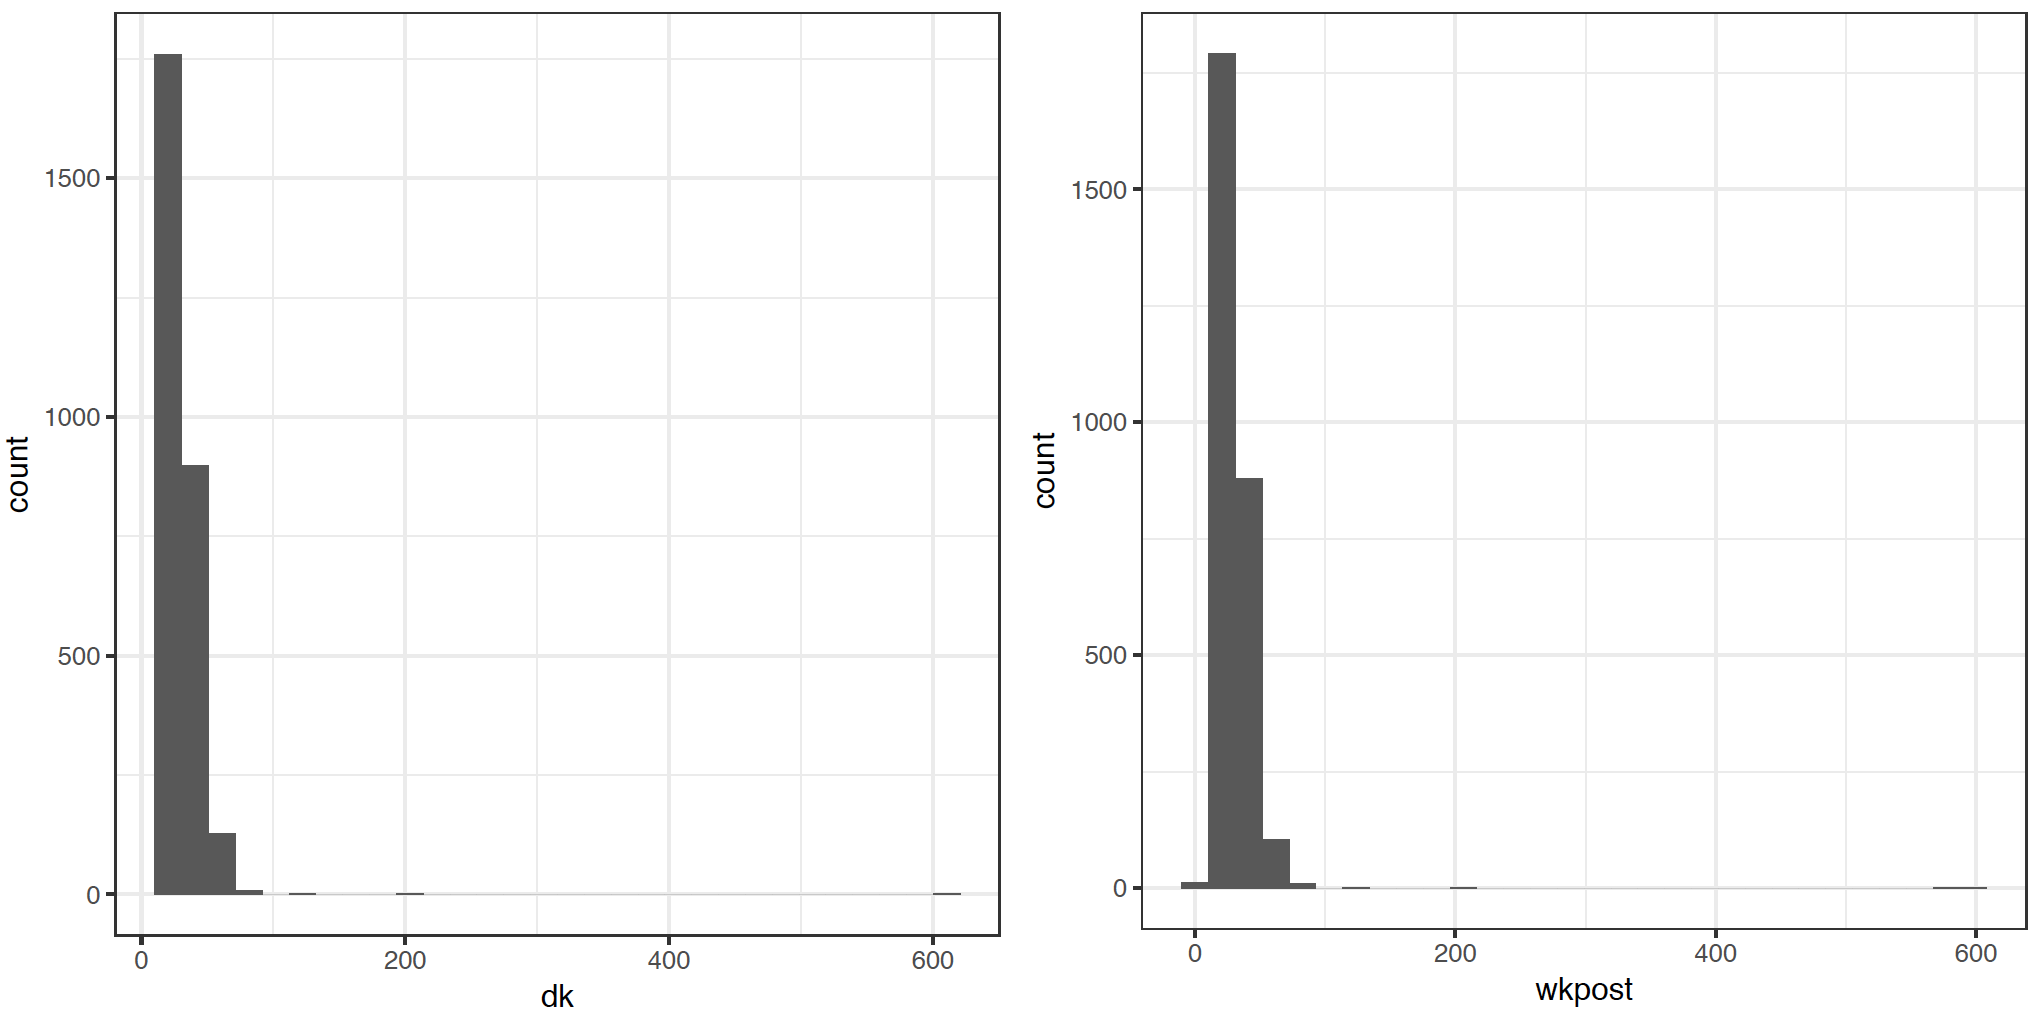
\includegraphics[width=\textwidth,height=5.20833in]{Pics/18.png}
\caption{\emph{Comparación de la distribución de los pesos básicos de muestreo (izquierda) con los pesos ajustados por ausencia de respuesta (derecha) en una encuesta de hogares.}}
\end{figure}

La teoría afirma que entre más variables de calibración se tengan menor será la varianza asociada a las estimaciones (no así el sesgo). Sin embargo, existen problemas computacionales cuando crecen las restricciones que se deben satisfacer son demasiadas. Una primera opción es verificar que no se tengan variables que puedan tener codependencia lineal con otras. Al descartar estas variables es posible conservar una varianza pequeña puesto que se descartan combinaciones lineales de otras variables.

Si los pesos de calibración resultan ser menores que uno su interpretación puede tornarse difícil (aunque no reviste un problema teórico). El usuario común entiende al factor de expansión como un factor de representatividad: \emph{es la cantidad de veces que una persona se represnta a sí misma y a algunas otras más en la población}. Por ende, los pesos negativos o menores que uno no resisten esta interpretación intuitiva y natural. Además, los pesos negativos pueden conllevar a estimaciones negativas para algunos dominios en donde el tamaño de muestra es pequeño, lo cual resulta ser problemático en un contexto en donde todas las variables de estudio son no negativas.

Para garantizar que los pesos se ubiquen en un intervalo determinado, se debe minimizar una distancia que a su vez debe inducir pesos restringidos a este intervalo y que respete las ecuaciones de calibración. Es posible que no se tenga una solución exacta para todas las restricciones de calibración e incluso que el algoritmo de calibración no converja. Nótese que los estimadores de calibración se pueden escribir como

\[
w_k = g_k * d_k
\]

Con base en lo anterior, es necesario analizar los pesos \(g_k\) en perspectiva en cada dominio, estrato y postestrato de interés. Una buena idea puede ser identificar aquellos \(g_k\) que resulten potencialmente grandes o influyentes. Se recomienda postestratificar la muestra, y aplicar la calibración a aquellas unidades en los que los \(g_k\) sean estables y usar los pesos originales en el restante conjunto.

Es posible hacer que los pesos de calibración estén restringidos a un espacio predefinido por el usuario, mediante límites \((L, U)\) sobre los \(g_k\). De esta forma, si \(w_k \geq 1\) implica \(g_k \geq 1\) y por tanto \(L=1\). Se acostumbra a tomar \(U > Q_3 + 1.5 * (Q_3 - Q_1)\) en donde \(Q_3\) y \(Q_1\) están dados en términos de la distribución de \(g_k\) y corresponden al tercer y primer cuartil, respectivamente.

Si el mecanismo que genera la ausencia de respuesta no es aleatorio (MAR) o completamente aleatorio (MCAR), es posible que los ponderadores de calibración induzcan sesgo en las estimaciones finales. En general, cuando hay ausencia de respuesta es más probable que aparezcan pesos de calibración negativos y que los pesos de calibración no convergieran a los pesos originales. Además, la varianza de los estimadores de calibración no convergerá a los resultados usuales de los estimadores de regresión.

\textcite{Silva_2004} presenta algunas medidas que permiten decidir cuáles escenarios de calibración son los mejores. A continuación se citan tales medidas.

\begin{itemize}
\item
  Error relativo promedio sobre las variables auxiliares
  \[
  M1= \frac{1}{p} \sum_{j=1}^p \frac{|\hat{t}_{xc} - t_x|}{t_x}
  \]
\item
  Coeficiente de variación HT relativo promedio
  \[M2= \frac{1}{p} \sum_{j=1}^p \frac{(Var(\hat{t}_{x\pi}))^{1/2}}{t_x} \]
\item
  Proporción de pesos extremos (límite inferior)
  \[M3 = \frac{1}{n} \sum_{k \in s}I(g_k<L)\]
\item
  Proporción de pesos extremos (límite superior)
  \[M4= \frac{1}{n} \sum_{k \in s}I(g_k>U)\]
\item
  Coeficiente de variación de los \(g_k\)
  \[M5= \frac{\sigma(g)}{\bar{g}}\]
\item
  Distancia entre los pesos de calibración y los pesos originales
  \[M6 = \frac{1}{n}\sum_{k \in s} \frac{(w_k - d_k)^2}{d_k}
  = \frac{1}{n}\sum_{k \in s} d_k(g_k - 1)^2\]
\item
  Eficiencia de los estimadores de calibración sobre la estimación del diseño de muestreo
  \[M7 = \frac{1}{J}\sum_{j=1}^J \frac{Var(\hat{t}_{y_jc})}{Var(\hat{t}_{y_j\pi})} \]
\item
  Efecto de la calibración sobre la dispersión de los ponderadores (DEFFk)
  \[M8 = 1+\frac{\sigma^2_w}{\bar{w}^2}\]
\end{itemize}

\hypertarget{calibracion-de-personas-con-bases-de-datos-de-hogares}{%
\subsubsection*{Calibración de personas con bases de datos de hogares}\label{calibracion-de-personas-con-bases-de-datos-de-hogares}}
\addcontentsline{toc}{subsubsection}{Calibración de personas con bases de datos de hogares}

Una de las preguntas recurrentes en la calibración de encuestas de hogares es el nivel al cual se debería realizar este ajuste. En prinicpio, es posible realizar la calibración al nivel de las personas, o al nivel de los hogares. Cada una de estas opciones trae algunas ventajas y consideraciones que se deben tener en cuenta.

Calibrar al nivel de los hogares implica que el hogar tendrá unos nuevos pesos que cumplen con las restricciones de calibración, y esos pesos los heredará a las personas que habitan el hogar. De esta forma todas las personas pertenecientes a un mismo hogar tendrán el mismo peso de muestreo, sin importar sus diferencias en composición demográfica. Es decir que, hombres, mujeres, menores y mayores de 15 años tendrán el mismo peso de muestreo. Esta propiedad es atractiva puesto que emula el diseño de muestreo que se definió en la fase de planeación. Por otro lado, realizar la calibración a nivel de los hogares hace que dentro de las unidades primarias de muestreo (UPMs) los hogares no tengan un peso homogeneo, lo que se distancia de las propiedades del diseño sistemático simple que se usa para la selección de los hogares dentro de las UPMs.

Por otro lado, calibrar a nivel de personas implica que los pesos de muestreo de los hogares también pueden verse alterados, y que los pesos finales de muestreo de las personas sean diferentes dentro de los hogares. De esta forma, de acuerdo a las características de las personas se tendrá un peso diferente. Es decir que hombres, mujeres, menores y mayores de 15 años \textbf{no} tendrían el mismo peso de muestreo. Por consiguiente cuando se calibra por personas y se utiliza un filtro sobre esa base de personas para crear una base de hogares, las características observadas de los jefes de hogares influenciarían los pesos d emuestreo resultantes en dicha base de datos de hogares.

En principio, se supone que se selecciona una muestra de unidades de una población finita \(U = \lbrace 1,2,\ldots,k,\ldots,M\rbrace\) la cual está agrupada en conglomerados \(U_I = \lbrace 1, 2,\ldots, i, \ldots, N_I \rbrace\). El proceso de selección se puede resumir de la siguiente manera \autocite{Gutierrez_2016}:

\begin{itemize}
\tightlist
\item
  Se selecciona una muestra \(S_I\) de conglomerados de \(U_I\) con probabilidades de inclusión \(\pi_{I_i}\) para \(i\in U_I\). Los pesos muestrales de la primera etapa son \(d_{I_i} = \frac{1}{\pi_{I_i}}\)
\item
  En la segunda etapa se seleccionan unidades para \(i\in S_I\). Se enumeran las unidades en \(U_i\) y se selecciona una muestra \(S_i\) con probabilidades de inclusión condicionales \(\pi_{k|i}\).
\item
  De esta forma, \(d_{k|i} = \frac{1}{\pi_{k|i}}\) son los pesos condicionales y \(d_k = d_{I_i}d_{k|i}\) es el peso de muestreo general para la k-ésima unidad, siendo \(s =\bigcup_{i\in s_I}S_i\) la muestra de unidades.
\end{itemize}

Para calibrar sobre la información auxiliar a nivel de hogar, se deben satisfacer las siguientes ecuaciones:

\[
\sum_{i \in S_I}w_{I_i}x_{ci} = \sum_{i \in U_I}x_{ci} = t_{x_c}
\]

En donde \(x_{ci}\) denota el vector de variables auxiliares a nivel del hogar, que siempre será definido como un conteo de individuos con cierta característica en el hogar. Por ejemplo, en su caso más básico \(x_{ci}\) puede ser el número de individuos en el hogar, mientras que el total auxiliar \(t_{x_c} = \sum_{i \in U_I}x_{ci}\) será el número de individuos en todos los hogares de Chile Luego de que se ha calibrado la base de hogares, se construyen los pesos a nivel de persona recurriendo a la siguiente expresión:

\[
w_k = d_{k|i}w_{I_i} \quad \forall k \in S_i
\]

Y además, se preserva la siguiente propiedad
\[
\frac{w_k}{w_{I_i}}=d_{k|i}
\]

Lo anterior imita la propiedad del muestreo en dos etapas de que

\[
\frac{d_k}{d_{I_i}}=d_{k|i}
\]

Como todos los individuos pertenecientes a un hogar son seleccionados para que respondan la encuesta de hogares, se tiene que \(d_{k|i} = 1\), por definición. Por lo tanto, el peso del individuo (en la base de datos de la muestra de personas) será idéntico al peso calibrado del hogar; es decir \(w_k = w_{I_i} \quad \forall k \in S_i\). Por lo anterior, dado que el muestreo es de conglomerados en la última etapa y todos los individuos del hogar son seleccionados, entonces el peso de muestreo del hogar será el promedio de los pesos individuales.

\[
w_{I_i}=\sum_{k\in S_i}\frac{w_k}{N_i}=\sum_{k\in U_i}\frac{w_k}{N_i}=\bar{w}_i
\]

Por último, nótese que la matriz de calibración toma la siguiente forma:

\[
X_{[i]}=X=
\begin{bmatrix}
x_{c11} & x_{c12} & \cdots & x_{c1p}\\
x_{c21} & x_{c22} & \cdots & x_{c2p}\\
x_{c31} & x_{c32} & \cdots & x_{c3p}\\
\vdots  & \vdots & \ddots &\\
x_{cN_I1} & x_{cN_I2} & \cdots & x_{cN_Ip}
\end{bmatrix}
\]

Por otro lado, la calibracion se puede realizar a nivel de las personas o a nivel de los hogares. Por ejemplo, si la calibración se realiza a nivel de personas y se calibra sobre la población en edad de trabajar, esto traerá como consecuencia que los factores de expansión sean diferentes para los miembros de un mismo hogar, puesto que la metodología buscará ajustar los totales de las personas en edad de trabajar y las personas que no están en la fuerza de trabajo de manera independiente. Por esta razón en la mayoría de hogares, en donde hay personas que son parte de la fuerza de trabajo y personas que no lo son, los pesos de muestreo no serán equivalentes. En principio, y debido al diseño de las encuesta, los pesos de muestreo originales son idénticos para todos los miembros de un mismo hogar. Sin embargo, cuando la calibración trata de ajustar los totales de las restricciones, y debido a que la población no está equitativamente distribuida, entonces de igual manera se presenta un reajuste en los factores de calibración. Por otro lado, calibrar a nivel de hogar hace que se cree un único factor de expansión para el hogar, que será heredado por todos sus miembros. Sin embargo, en este acercamiento y debido a que la composición de los hogares es diferente, entonces dentro de una misma UPM se tendrán hogares con diferentes pesos de muestreo.

En el caso particular en que haya información auxiliar disponible a nivel de personas y hogares (al mismo tiempo), es posible calibrar conjuntamente ambas variables en un sólo procedieminto de calibración. \textcite[sec.~5]{Estevao_Sarndal_2006} recrea la calibración conjunta para hogares y personas, en donde se genera una variable indicadora para el jefe de hogar y sobre esta se crea una nueva restricción de calibración que utilice los totales auxiliares de los hogares. Con esta nueva calibración, se generan unos nuevos pesos de calibración en la base de datos de personas. Al filtrar esta base de datos por el jefe de hogar, se crea inmediatamente una base de hogares (puesto que solo hay un único jefe de hogar) que puede ser utilizada para combinarla con la información de los hogares. De esta forma, los pesos que venían de la base de datos de personas serán los que se utilicen en la base de datos de hogares obteniendo estimaciones consistentes.

\hypertarget{estimadores-y-error-de-muestreo}{%
\chapter{Estimadores y error de muestreo}\label{estimadores-y-error-de-muestreo}}

\hypertarget{estimadores-puntuales}{%
\section{Estimadores puntuales}\label{estimadores-puntuales}}

La mayoría de indicadores sociales a nivel nacional pueden verse como funciones de totales de una o más variables de interés. Por ejemplo, si el interés está en estimar un total \(t_y=\sum_U y_k\), el estimador de expansión provee una metodología que induce insesgamiento.

\[
\hat{t}_y = \sum_s w_k y_k
\]

En donde la muestra \(s\) hace referencia al subconjunto de la población que fue seleccionado siguiendo un diseño de muestreo probabilístico que induce los pesos de muestreo \(w_k\) que expanden el valor de la variable de interés \(y_k\) para el \(k\)-ésimo individuo. Nótese que \(w_k\) es función de la probabilidad de inclusión de \(k\)-ésimo individuo en la muestra \(\pi_k=Pr(k\in s)\). En presencia de esquemas de estratificación y selección de conglomerados y varias etapas, esta probabilidad resulta ser el producto de las probabilidades condicionales que surgen en los subsecuentes procesos de selección probabilística. Por tanto, el peso final de muestreo resulta ser por lo general una multiplicación de factores de expansión en cada etapa del esquema de muestreo.

Por ejemplo, si el diseño de la encuesta es estratificado por regiones \(h\) (agrupaciones de municipios), con tres etapas de selección dentro de cada estrato (la primera etapa con selección de municipios \(i\) dentro del estrato, la segunda con selección de segmentos cartográficos \(j\) y la última con selección de hogares \(k\)), entonces el peso de muestreo final y el estimador del total estará dado por la siguiente expresión

\[
\hat{t}_y = \sum_s w_j y_k = \sum_h \sum_{i \in s_h} \sum_{j \in s_{hi}} \sum_{k \in s_{hij}} w_{hijk} y_{hijk}
\]

En presencia de información auxiliar es posible mejorar la eficiencia de la estimación acudiendo a diferentes formas funcionales que estiman el total, por ejemplo, con el estimador de Hájek:

\[
\hat{t}_y = t_x \frac{\sum_s w_k y_k}{\sum_s w_k x_k}
\]

En donde \(t_x\) denota el total poblacional, que se supone conocido para toda la población, de una variable auxiliar \(x\) que es preguntada en la encuesta de hogares. Por supuesto, en el análisis de este tipo de encuestas es común realizar inferencias sobre parámetros que tienen una forma no lineal. Uno de los más básicos es la razón poblacional \(R_U = t_{y_1} / t_{y_2}\) cuya estimación se lleva a cabo estimando ambos componentes de la fracción

\[
\hat{R}= \frac{\hat{t}_{y_1}}{\hat{t}_{y_2}}
= \frac{\sum_s w_k y_{1k}} {\sum_s w_k y_{2k}}
\]

La estimación de un promedio poblacional \(\bar{y}_U = t_y / N\), se lleva a cabo de forma eficiente estimando el tamaño de la población y se puede ver como un caso particular de la estimación de una razón

\[
\hat{\bar{y}}_s= \frac{\hat{t}_y}{\hat{N}} 
= \frac{\sum_s w_k y_k}{\sum_s w_k}
\]

Las encuestas de hogares con diseños panel o rotativos, tienen un mayor interés en la estimación del cambio de indicadores en dos periodos tiempo \(\Delta = t_y^{(t)} - t_y^{(t-1)}\). Nótese que un estimador de este parámetro está dado por

\[
\hat{\Delta} = \hat{t}_{y^{(t)}} - \hat{t}_{y^{(t-1)}}
\]

Además, es posible mejorar la estimación del total actual \(t_y^{(t)}\) al tener en cuenta la información inducida por el traslape de la encuesta en el segundo periodo, así:

\[
\tilde{t}_{y^{(t)}} = \alpha \hat{t}_{y^{(t)}} 
+ (1 -\alpha) (\tilde{t}_{y^{(t-1)}} - \hat{\Delta})
\]

En donde \(0 < \alpha < 1\). Por otro lado, si el interés está en estimar algunas características asociadas con la pobreza, es posible utilizar estimadores más complejos. Siendo \(y_k\) el ingreso del individuo \(k\) y \(l\) el umbral de pobreza, entonces el siguiente estimador puede ser utilizado

\[
\hat{F}_{\alpha}=\frac{1}{N}\sum_{k\in s} w_k 
\left(\frac{l-y_k}{l}\right)^{\alpha}I(y_k<l)
\]

En donde \(I(y_k<l)\) es una variable indicadora que toma el valor uno si \(y_k<l\) o cero, en cualquier otro caso. Note que si \(\alpha = 0\), se tiene una estimación de la incidencia de la pobreza y si \(\alpha = 1\), se obtiene un estimación de la brecha de la pobreza \autocite{Foster_Greer_Thorbecke_1984}.

La selección del estimador está altamente relacionada con el diseño de la encuesta. Por ejemplo, si se pretende estimar un indicador para un periodo de tiempo definido, el diseño de la encuesta no debería inducir un esquema de rotación que tenga traslape de hogares, puesto que la correlación del indicador induciría un aumento de su varianza y por ende pérdida de eficiencia. Sin embargo, si se desea estimar el cambio del indicador entre dos periodos de tiempos, es necesario contar con un esquema de rotación que asegure un tamaño de muestra suficiente para estimar con precisión este cambio. \textcite[sección 12.13]{Cochran_1977} afirma que, cuando el interés se centra tanto en la estimación del indicador en el periodo actual como en la estimación del cambio entre periodos, es recomendable tener una tasa de traslape de 2/3, 3/4 o 4/5 de una ronda a otra.

\hypertarget{estimacion-del-error-de-muestreo}{%
\section{Estimación del error de muestreo}\label{estimacion-del-error-de-muestreo}}

Aunque la escogencia del diseño de muestreo y el estimador sean de libre elección para los investigadores, no lo es el cálculo de las medidas de confiabilidad y precisión. Dado que la base científica sobre la cual descansa el muestreo es la inferencia estadística, se deben respetar las normas básicas para la asignación y posterior cálculo del margen de error, que constituye una medida unificada del error total de muestreo que cuantifica la incertidumbre acerca de las estimaciones en una encuesta.

\hypertarget{la-tecnica-del-ultimo-conglomerado}{%
\subsection{La técnica del último conglomerado}\label{la-tecnica-del-ultimo-conglomerado}}

Debido a las dificultades algebricas y computacionales, estimar la varianza en encuestas complejas que contemplan esquemas de conglomeración, selección en varias etapas y estratifcación, puede tornarse bastante tedioso, costoso y además muy demorado. En este documento se explica por qué la técnica del último conglomerado resulta ser una buena opción a la hora de aproximar la varianza en una encuesta compleja.

Para la estimación de la varianza de los estimadores de interés en encuestas multi-etápicas, los programas computacionales existentes utilizan una aproximación conocida como la técnica del último conglomerado. Esta aproximación, que sólo tiene en cuenta la varianza de los estimadores en la primera etapa, supone que ese muestreo fue realizado con reemplazo. Los procedimientos de muestreo en etapas posteriores de la selección son ignorados a menos que el factor de corrección para poblaciones finitas sea importante a nivel municipal.

En particular considere cualquier estimador del total poblacional dado por la siguiente combinación lineal

\begin{equation}
\label{est}
\hat{t}_{y}=\sum_{k\in s} d_k y_k = \sum_{k\in U} I_k d_k y_k 
\end{equation}

En donde \(I_k\) son variables indicadoras de la pertenecia del elemento \(k\) a la muestra \(s\). Ahora, asumamos que el factor de expansión de la encuesta \(d_k\) cumple con los supuestos básicos de un ponderador que hace insesgado a \(\hat{t}_{y}\), es decir:

\begin{equation*}
E_p(I_k d_k) = 1
\end{equation*}

Se supone un diseño de muestreo en varias etapas (dos o más) en donde la primera etapa supone la selección de una muestra \(s_I\) de \(m_I\) unidades primarias de muestreo (UPM) \(U_i\) (\(i\in s_I\)) de tal forma que

\begin{itemize}
\tightlist
\item
  Si la selección se realizó con reeemplazo, la \(i\)-ésima UPM tiene probabhilidad de selección \(p_{I_i}\).
\item
  Si la selección se realizó sin reeemplazo, la \(i\)-ésima UPM tiene probabilidad de inclusión \(\pi_{I_i}\).
\end{itemize}

En las subsiguientes etapas de muestreo, se procede a seleccionar una muestra de elementos para cada una de las UPM seleccionadas en la primera etapa de muestreo. Dentro de la \(i\)-ésima UPM se selecciona una muestra \(s_i\) de elementos; en particular la probabilidad condicional de que el \(k\)-ésimo elemento pertenzca a la muestra dada que la UPM que la contiene ha sido seleccionada en la muestra de la primera etapa está dada por la siguiente expresión:

\begin{equation*}
\pi_{k|i} = Pr(k \in s_i | i \in s_I)
\end{equation*}

Por ejemplo, si el muestreo es sin reemplazo en todas sus etapas, la probabilidad de inclusión del \(k\)-ésimo elemento a la muestra \(s\) está dada por

\begin{align*}
\label{piki}
\pi_k & = Pr(k \in s)\\ 
& = Pr(k \in s_i, i \in s_I) \\
& = Pr(k \in s_i | i \in s_I) Pr(i \in s_I) = \pi_{k|i} \times \pi_{I_i}
\end{align*}

Dado que el inverso de las probabilidades de inclusión son un ponderador natural, entonces se definen las siguientes cantidades:

\begin{enumerate}
\def\labelenumi{\arabic{enumi}.}
\tightlist
\item
  \(d_{I_i} = \frac{1}{\pi_I}\), que es el factor de expansión de la \(i\)-ésima UPM.
\item
  \(d_{k|i} = \frac{1}{\pi_{k|i}}\), que es el factor de expansión del \(k\)-ésimo elemento dentro para la \(i\)-ésima UPM.
\item
  \(d_k = d_{I_i} \times d_{k|i}\), que es el factor de expansión final del \(k\)-ésimo elemento para toda la población \(U\).
\end{enumerate}

\textbf{Resultado}: \emph{Bajo un diseño de muestreo en varias etapas, el estimador de Hansen-Hurwitz para el total poblacional está dada por:}
\begin{equation}
\label{HH}
\hat{t}_{y,p}=\frac{1}{m_I}\sum_{i=1}^{m_I}\frac{\hat{t}_{y_i}}{p_{I_i}}
\end{equation}

\emph{Y su varianza estimada es:}
\begin{equation}
\label{var}
\widehat{Var}(\hat{t}_{y,p})=\frac{1}{m_I(m_I-1)}\sum_{i=1}^{m_I}\left(\frac{\hat{t}_{y_i}}{p_{I_i}}-\hat{t}_{y,p}\right)^2
\end{equation}

Supongamos ahora que la encuesta tiene un diseño complejo \(p(s)\) que no contempla reeemplazo en la primera etapa. Por lo tanto, algunas cantidades deben ser equiparadas para poder utilizar esta aproximación. En principio, nótese que las cantidades \(\hat{t}_{y_i}\) representan lo totales estimados de la variable de intereés en la \(i\)-ésima UPM y están dados por:

\begin{equation}
\hat{t}_{y_i} = \sum_{k \in s_i} \frac{y_k}{\pi_{k|i}}
= \sum_{k \in s_i} d_{k|i} y_k 
\end{equation}

Utilizar la aproximación de la varianza requiere equiparar los términos de manera apropiada. En primer lugar, fijémonos en los estimadores dados por \eqref{HH} y \eqref{est}. Para realizar esta comparación, se requiere que
se asuma la siguiente igualdad en las probabilidades de inclusión de la primera etapa:

\begin{equation}
\label{cons}
\pi_{I_i} = p_{I_i} \times m_I 
\end{equation}

Por lo tanto, el estimador del total poblacional quedaría definido desde \eqref{est} como un estimador tipo Hanwen-Hurwitz.

\begin{align*}
\hat{t}_{y} =\sum_{k\in s} d_k y_k  
= \sum_{i=1}^{m_I}\sum_{k \in s_i} d_k y_k 
= \sum_{i=1}^{m_I}\sum_{k \in s_i} \frac{1}{\pi_{I_i} \pi_{k|i}} y_k 
= \sum_{i=1}^{m_I}\frac{\hat{t}_{y_i}}{\pi_{I_i}} 
\approx \frac{1}{m_I}\sum_{i=1}^{m_I}\frac{\hat{t}_{y_i}}{p_{I_i}}
\end{align*}

Ahora, dado que la forma del estimador ha sido equiparada con un estimador tipo Hanwen-Hurwitz, es posible utilizar su estimación de varianza. Aún más, después de un poco de álgebra y tuilizando la equiparación dada por \eqref{cons}, es posible tener la siguiente aproximación, cuya gran ventaja es que sólo hace uso de los factores de expansión finales \(d_k\), que suelen ser reportados por los Institutos Nacionales de Estadística cuando liberan los microdatos de sus encuestas, en vez de los factores de expansión de la primera etapa o los factores de expansión condicionales dentro de las UPM.

\begin{align*}
\widehat{Var}(\hat{t}_{y,p})&=\frac{1}{m_I(m_I-1)}\sum_{i=1}^{m_I}\left(\frac{\hat{t}_{y_i}}{p_{I_i}}-\hat{t}_{y}\right)^2\\
&=\frac{m_I}{m_I-1}\sum_{i=1}^{m_I}\frac{1}{m_I^2}\left(\frac{\sum_{k \in s_i} d_{k|i} y_k }{p_{I_i}}-\sum_{i=1}^{m_I}\sum_{k \in s_i} d_k y_k \right)^2 \\
&=\frac{m_I}{m_I-1}\sum_{i=1}^{m_I}\left(\frac{\sum_{k \in s_i} d_{k|i} y_k }{m_I p_{I_i}}-\frac{1}{m_I}\sum_{i=1}^{m_I}\sum_{k \in s_i} d_k y_k \right)^2 \\
&=\frac{m_I}{m_I-1}\sum_{i=1}^{m_I}\left(\frac{\sum_{k \in s_i} d_{k|i} y_k }{\pi_{I_i}}-\frac{1}{m_I}\sum_{i=1}^{m_I}\sum_{k \in s_i} d_k y_k \right)^2 \\
&=\frac{m_I}{m_I-1}\sum_{i=1}^{m_I}\left( \sum_{k \in s_i} d_k y_k -\frac{1}{m_I}\sum_{i=1}^{m_I}\sum_{k \in s_i} d_k y_k \right)^2 
\end{align*}

Basado en lo anterior, al definir \(\breve{t}_{y_i} = \sum_{k \in s_i} d_k y_k\) como la contribución\footnote{Note que la suma de estas contribuciones en la muestra de la primera etapa da como resultado la estimación \(\hat{t}_y\).} de la \(i\)-ésima UPM a la estimación del total poblacional y \(\bar{\breve{t}}_{y}=\frac{1}{m_I}\sum_{i=1}^{m_I}\breve{t}_{y_i}\) como la contribución promedio en el muestreo de la primera etapa, entonces el estimador de varianza toma la siguiente forma, conocida como el estimador de varianza del \textbf{último conglomerado}.

\begin{align}
\label{UC}
\widehat{Var}(\hat{t}_{y,p})
=\frac{m_I}{m_I-1}\sum_{i=1}^{m_I}\left( \breve{t}_{y_i} -\frac{1}{m_I}\sum_{i=1}^{m_I}\breve{t}_{y_i} \right)^2 
=\frac{m_I}{m_I-1}\sum_{i=1}^{m_I}\left( \breve{t}_{y_i} - \bar{\breve{t}}_{y} \right)^2
\end{align}

Siguiendo con el escenario de muestreo planteado en las secciones anteriores, si el diseño de la encuesta es estratificado por regiones \(h\), con tres etapas de selección dentro de cada estrato, entonces al utilizar la técnica del último conglomerado, el estimador de la varianza de \(\hat{t}_{y}\) estaría dado por

\[
\hat{V}(\hat{t}_{y}) = 
\sum_h\frac{n_h}{n_h-1}\sum_{i\in s_h}\left(\hat{t}_{y_i}-\bar{\hat{t}}_{y_h}\right)^2
\]

En donde \(\hat{t}_{y_i} = \sum_{k \in s_{hi}} w_k y_k\), \(\bar{\hat{t}}_{y_h}=(1/n_h)\sum_{i \in s_h}\hat{t}_{y_i}\) y \(n_h\) es el número de UPMs seleccionadas en el estrato \(h\). Este procedimiento, propuesto por \textcite{hansen1953sample} tiende a sobrestimar la varianza verdadera, aunque resulta ser una técnica apetecida por los investigadores puesto que utiliza directamente los pesos finales de muestreo o factores de expansión que son publicados por los INE.

Utilizar la técnica del \textbf{último conglomerado} es una salida práctica al problema de la estimación de la varianza que, para la mayoría de encuestas que brindan estadísticas oficiales a los países, puede tornarse bastante complejo. Si bien, la expresión \eqref{UC} no brinda estimaciones de varianza estrictamente insesgadas, sí constituye una aproximación bastante precisa.

¿Qué es un \textbf{último conglomerado}? Es la primera unidad de muestreo en un diseño complejo. Por ejemplo, considere el siguiente diseño de muestreo en cuatro etapas:

\begin{equation*}
\underbrace{\textbf{Municipio}}_{\text{UPM}} \Rrightarrow
\underbrace{\textbf{Sector}}_{\text{USM}} \Rrightarrow
\underbrace{\textbf{Vivienda}}_{\text{UTM}} \Rrightarrow
\underbrace{\textbf{Hogar}}_{\text{UFM}}
\end{equation*}

En la primera las unidades primarias de muestreo (UPM) son los municipios; dentro de cada municipio, se seleccionan unidades secundarias de muestreo (USM) que corresponden a sectores cartográficos; de esta forma, el submuestreo continua hasta seleccionar las unidades finales de muestreo (UFM) que son los hogares.

Ahora, por lo general, la primera etapa de muestreo de una encuesta está inducida por dos tipos de diseños: estratificado o con probabilidad de selección proporcional al tamaño del municipio. En cualquiera de los dos casos, se cren subgrupos de inclusión forzosa. En el muestreo estratificado serán las ciudades grandes y en el muestreo proporcional también, puesto que la medida de tamaño inducira probabilidades de inclusión mayores a uno.
Luego, los municipios pertenecientes a este subgrupo de inclusión forzosa no pueden ser condierados como UPM, sino como un estrato de ciudades grandes. En cada ciudad de este estrato se realizará un muestreo de la siguiente manera:

\begin{equation*}
\underbrace{\textbf{Sector}}_{\text{UPM}} \Rrightarrow
\underbrace{\textbf{Vivienda}}_{\text{USM}} \Rrightarrow
\underbrace{\textbf{Hogar}}_{\text{UFM}}
\end{equation*}

Es necesario tener en cuenta esta particularidad de las encuestas para poder aplicar correctamente esta técnica de aproximación de varianzas. En resumen, para aquellas ciudades que pertenecen al estrato de inclusión forsoza, las UPM serán los sectores cartográficos, y para el resto del país, las UPM serán los municipios cuya probabilidad de inclusión en la muestra de la primera etapa es menor a uno.

\hypertarget{linealizacion-de-taylor}{%
\subsection{Linealización de Taylor}\label{linealizacion-de-taylor}}

Cuando se trata de estimar parámetros que tienen una forma no lineal, es posible recurrir al uso de las herramientas del análisis matemático para aproximar sus varianzas con el fin de publicar las cifras oficiales con sus respectivos errores estándar. \textcite{Valliant_Dever_Kreuter_2013} mencionan que esta técnica se basa en expresar el estimador como función de estimadores lineales de totales. Por ejemplo, si el interés recae en estimar un parámetro poblacional \(\theta\) que a su vez depende de \(p\) estimadores lineales, entonces su estimador de muestreo se debe expresar como

\[
\hat{\theta}=f(\hat{t}_1, \ldots, \hat{t}_p)
\]

En donde \(\hat{t}_j=\sum_{k\in s}w_k y_{jk}\) es un estimador del \(j\)-ésimo total. La linealización de Taylor supone que es posible definir una aproximación lineal de \(\hat{\theta}\) así

\[
\hat{\theta} - \theta 
\approx \sum_{j=1}^p \frac{\partial f(\hat{t}_1, \ldots, \hat{t}_p) }{\partial \hat{t}_j}(\hat{t}_j - t_j)
= \sum_{k\in s} w_k z_k + c
\]

En donde \(z_k= \sum_{j=1}^p \frac{\partial f(\hat{t}_1, \ldots, \hat{t}_p) }{\partial \hat{t}_j} y_{jk}\) son variables linealizadas y \(c\) son constantes determinísticas que por consiguiente no aportan a la varianza de \(\hat{\theta}\). Nótese lo conveniente de expresar esta aproximación de esta manera puesto que al final, las cantidades que intervienen en la varianza se pueden expresar como una suma ponderada de las variables \(z_k\) y por consiguiente es posible aplicar todos los principios establecidos anteriormente. De esta forma, asumiendo el escenario de muestreo planteado en las secciones anteriores, el estimador de la varianza de la aproximación lineal de \(\hat{\theta}\) está dado por

\[
\hat{V}(\hat{\theta}) = 
\sum_h\frac{n_h}{n_h-1}\sum_{i\in s_h}\left(\hat{t}_{z_i}-\bar{\hat{t}}_{z_h}\right)^2
\]

En donde \(\hat{t}_{z_i} = \sum_{k \in s_{hi}} w_k z_k\) y \(\bar{\hat{t}}_{z_h}=(1/n_h)\sum_{i \in s_h}\hat{t}_{z_i}\). Por ejemplo, si el interés estuviera en estimar una razón, entonces las nuevas variables linealizadas son \(z_k=(1/\hat{t}_{y_2})(y_{1k}-\hat{\theta}y_{2k})\).

En la región la \emph{Pesquisa Nacional por Amostra de Domicilios Continua}, en Brasil, y la \emph{Encuesta de Caracterización Socioeconómica Nacional}, en Chile, utilizan esquemas de linealización de Taylor en conjunción con el acercamiento del último conglomerado.

\hypertarget{replicas}{%
\subsection{Réplicas}\label{replicas}}

Las complicaciones en el cálculo de los errores de muestreo pueden ser mayores dependiendo de la escogencia del estimador y del diseño de muestreo asumido para la recolección de la información primaria. En algunas ocasiones, el proceso de linealización puede resultar complicado, por lo que es posible optar por una estrategia computacional aproximada que permite pasar por alto el proceso teórico de definición de las cantidades que estiman la varianza del estimador. Este conjunto de métodos supone la idea de la selección sistemática de \emph{submuestras} que son utilizadas para estimar el parámetro de interés, utilizando los mismos principios de estimación que con la muestra completa. Por lo anterior, se obtienen estimaciones puntuales para cada réplica, las cuales son utilizadas para estimar la varianza del estimador de interés.

En particular, hay tres metodologías que abordan este problema: las réplicas repetidas balanceadas \autocites{McCarthy_1969}{Judkins_1990}, el Jackknife \autocite{Krewski_Rao_1981} y el Bootstrap \autocite{Rao_Wu_1988}. La idea general detrás de estos métodos es que, partiendo de la muestra completa, en cada réplica se seleccione un conjunto de UPMs manteniendo todas las unidades que hayan sido seleccionadas dentro de esas UPMs. Luego, es necesario reponderar los pesos de muestreo para que se conserve la representatividad; de esta manera, para cada réplica se obtendrá un nuevo conjunto de pesos de muestreo. Con estos pesos, se calcula la estimación de interés, obteniendo tantas estimaciones como réplicas definidas. \textcite{Wolter_2007} provee todos los detalles teóricos referentes al problema de la estimación de la varianza utilizando réplicas.

Por ejemplo, al utilizar la técnica de Jackknife, y asumiendo el escenario de muestreo planteado en las secciones anteriores (estratificado con varias etapas de muestreo), si se quiere estimar el error asociado a una medida de pobreza estimada, entonces se eliminará la primera UPMs del primer estrato para formar la primera réplica, luego la segunda UPMs del primer estrato para formar la segunda réplica y así sucesivamente hasta que se hayan formado todas las réplicas necesarias. De esta forma, si la UPMs \(i\) del estrato \(h\) fue eliminada, se deben crear los siguientes pesos de muestreo para las unidades que permanecen en la submuestra

\[
w_{k}^{(hi)} = 
\begin{cases}
0, & \text{si $k$ pertenece a la UPMs $i$ del estrato $h$.} \\
\frac{n_h}{n_h-1}w_k, & \text{si $k$ pertenece a la UPMs $i$ del estrato $h$.} \\
w_k, & \text{si $k$ no pertenece al estrato $h$.} 
\end{cases}
\]

Con cada nuevo conjunto de pesos, es necesario estimar la medida de pobreza requerida utilizando la siguiente expresión:

\[
\hat{F}_{\alpha}^{(hi)}=\frac{1}{N}\sum_{k\in s^{(hi)}} w_k^{(hi)} 
\left(\frac{l-y_k}{l}\right)^{\alpha}I(y_k<l)
\]

En donde \(s^{(hi)}\) hace referencia al subconjunto de la muestra inducida por la réplica al eliminar la UPMs \(i\) del estrato \(h\). Luego, de obtener cada una de las estimaciones, la varianza de \(\hat{F}_{\alpha}\) será estimada de la siguiente manera

\[
\hat{V}_{J}(\hat{F}_{\alpha})=\sum_{h}\frac{n_h-1}{n_h}
\sum_{i\in s_h} \left(\hat{F}_{\alpha}^{(hi)} - \hat{F}_{\alpha}\right)
\]

En lo concerniente con las técnicas de remuestreo y la utilización de las réplicas para el cálculo de los errores de muestreo se recalca que la técnica de \emph{Jackknife} es útil para estimar parámetros lineales, pero no tiene un buen comportamiento cuando se trata de estimar percentiles o funciones de distribución. La técnica de \emph{réplicas repetidas balanceadas} es útil para estimar parámetros lineales y no lineales, pero puede ser deficiente cuando se tienen dominios pequeños que pueden inducir estimaciones nulas en la configuración de los pesos. Sin embargo, el ajuste de Fay a la técnica anterior resulta palear todos los anteriores inconvenientes. En este caso es importante utilizar una matriz de Hadammard que induzca no más de 120 réplicas para que la publicación de la base de datos no se sobrecargue. Por último, el \emph{bootstrap} debe ser utilizado con con detenimiento porque debe replicar el diseño de muestreo exacto y esto se hace construyendo una población a partir de los pesos de muestreo.

XXXX

Las fórmulas computacionales requeridas para estimar la varianza de estadísticas descriptivas como la media muestral están disponibles para algunos diseños complejos que incorporan elementos como la estratificación y el muestreo por conglomerados. Sin embargo, en el caso de estadísticas analíticas más complejas, tales como coeficientes de correlación y coeficientes de regresión, no se encuentra fácilmente las fórmulas específicas en diseños muestrales que se aparten del muestreo aleatorio simple. Estas fórmulas son enormemente complicadas o, en última instancia, se resisten al análisis matemático (Frankel, 1971).

En ausencia de fórmulas adecuadas, en los últimos años han aparecido una variedad de técnicas empíricas que proporcionan \emph{varianzas aproximadas que parecen satisfactorias para fines prácticos} (Kish, 1995). Estos métodos utilizan una muestra de datos para construir submuestras y generar una distribución para las estimaciones de los parámetros de interés utilizando cada submuestra. Los resultados de la submuestra se analizan para obtener una estimación del parámetro, así como intervalos de confianza para esa estimación.

Entre los métodos de muestreo, se encuentran principalmente la técnica de Jackknife, el método de las Réplicas Repetidas Balanceadas (RRB) y el método de Bootstrap.

\hypertarget{la-tecnica-de-jackknife}{%
\subsubsection*{La técnica de Jackknife}\label{la-tecnica-de-jackknife}}
\addcontentsline{toc}{subsubsection}{La técnica de Jackknife}

Es posible estimar la varianza de los estimadores de interés usando la técnica de Jackknife. El desarrollo del procedimiento de Jackknife se remonta a un método utilizado por Quenouille (1956) para reducir el sesgo de las estimaciones. El refinamiento ulterior del método (Mosteller \& Tukey, 1968) llevó a su aplicación en una serie de situaciones de las ciencias sociales en las que las fórmulas no están fácilmente disponibles para el cálculo de errores de muestreo.

Este procedimiento ofrece los siguientes beneficios:

\begin{enumerate}
\def\labelenumi{\arabic{enumi}.}
\tightlist
\item
  \emph{Mayor flexibilidad}: el Jackknife puede implementarse en una amplia variedad de diseños muestrales.
\item
  \emph{Facilidad de uso}: el Jackknife no requiere de software especializado.
\end{enumerate}

El concepto principal de esta técnica parte de una muestra de tamaño \(n\), la cual se divide en \(A\) grupos de igual
tamaño \(m=n/A\), a partir de esta división, la varianza de un estimador \(\hat{\theta}\) se estima a partir de la varianza observada en los \(A\) grupos.

Para cada grupo \((a=1,2,...,A)\), se calcula \(\hat{\theta}_{(a)}\), una estimación para el parámetro \(\theta\), calculada de la misma forma que la estimación \(\hat{\theta}\) obtenida con la muestra completa, pero solo con la información restante (luego de la eliminación del grupo \(a\)). Para \(a=1,2,...,A\) se define

\[\hat{\theta}_{a}=A\hat{\theta}-(A-1)\hat{\theta}_{(a)}\]

como un pseudovalor de \(\theta\). El estimador obtenido mediante Jackknife se presenta como una alternativa a \(\hat{\theta}\) y se define como:

\[\hat{\theta}_{JK}=\dfrac{1}{A}\sum_{a=1}^{A}\hat{\theta}_{a}\]

mientras que el estimador de la varianza obtenido mediante Jackknife se obtiene como:

\[\hat{V}_{JK1}=\dfrac{1}{A(A-1)}\sum_{a=1}^{A}\left(\hat{\theta}_{a}-\hat{\theta}_{JK}\right)^{2}\]

También es posible utilizar como estimador alternativo:

\[\hat{V}_{JK2}=\dfrac{1}{A(A-1)}\sum_{a=1}^{A}\left(\hat{\theta}_{a}-\hat{\theta}\right)^{2}\]

Para diseños estratificados y multietápicos en los cuales unidades primarias de muestreo han sido seleccionadas en el estrato \(h\), para \(h=1, \ldots, H\), el estimador de varianza de Jackknife para la estimación de un parámetro poblacional está dado por

\[ \hat{V}_{JK}(\hat{\theta}) = \sum_{h=1}^H \frac{n_h - 1}{n_h} \sum_{i=1}^{n_h}
(\hat{\theta}_{(hi)}-\hat{\theta})^2\]

donde \(\hat{\theta}_{(hi)}\) es la estimación de \(\theta\) usando los datos de la muestra excluyendo las observaciones en la \(i\)-ésima unidad primaria de muestreo (Korn \& Graubard, 1999, pg. 29 -- 30). Shao \& Tu (1995, Teorema 6.2) garantiza la convergencia en probabilidad de este estimador hacia la varianza teórica, de donde se puede concluir que es un estimador aproximadamente insesgado para la varianza teórica. Computacionalmente, se puede obtener la estimación Jackknife por medio de la creación de la base de datos omitiendo las observaciones necesarias usando comando \texttt{as.svrepdesign} de la librería \texttt{survey} del software estadístico `R para calcular \(\hat{V}_{JK}(\hat{\theta})\), y posteriormente calcular el valor de la estimación Jackknife.

En el contexto de este estudio, se tiene un número relativamente grande de unidades primarias de muestreo: 289 escuelas para el grado tercero y 287 para el grado sexto, por lo que el método de Jackknife puede ser un poco ineficiente puesto que implica la creación de 289 réplicas para el grado tercero y 287 réplicas para el sexto, por lo cual se recurrirá otro método de remuestreo, presentado más adelante, donde el usuario define el número de réplicas.

\begin{figure}
\centering
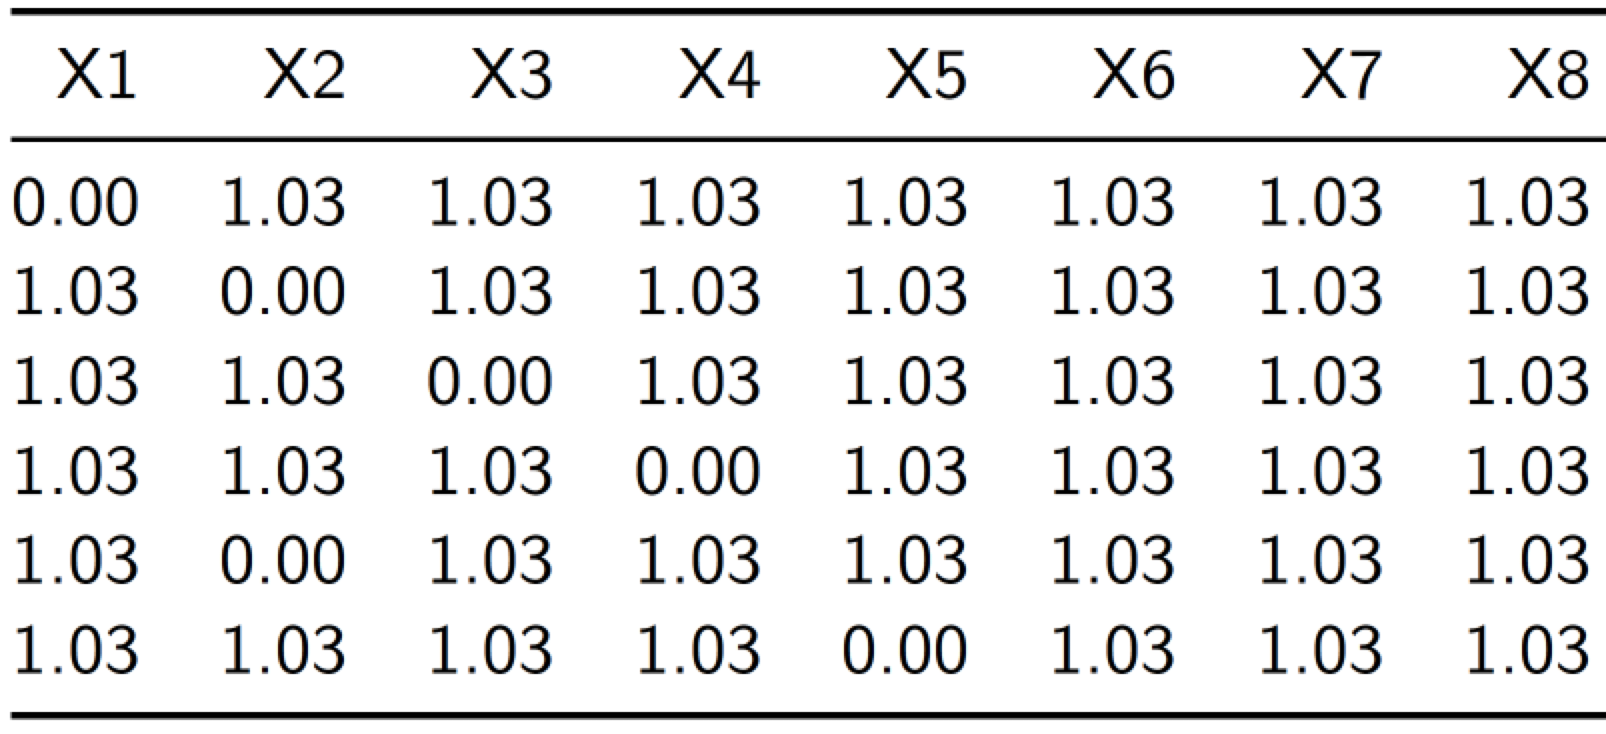
\includegraphics{Pics/20.png}
\caption{\emph{Primeras ocho réplicas del método de JacKnife.}}
\end{figure}

\hypertarget{el-metodo-de-las-replicas-repetidas-balanceadas}{%
\subsubsection*{El método de las Réplicas Repetidas Balanceadas}\label{el-metodo-de-las-replicas-repetidas-balanceadas}}
\addcontentsline{toc}{subsubsection}{El método de las Réplicas Repetidas Balanceadas}

Las varianzas de muestreo tabmién pueden ser calculadas haciendo uso del método conocido como Réplicas Repetidas Balanceadas, el cual permite explicar la varianza que se obtiene en las estimaciones debido al muestreo. Este método es el que utilizan pruebas internacionales como PISA para realizar los análisis de datos. Bajo la metodología BRR, el estimador de la varianza toma la siguiente forma:
\[
Var(\hat{\theta}) = \frac{1}{A}\sum_{a=1}^A(\hat{\theta}_a - \hat\theta )^2
\]

\begin{figure}
\centering
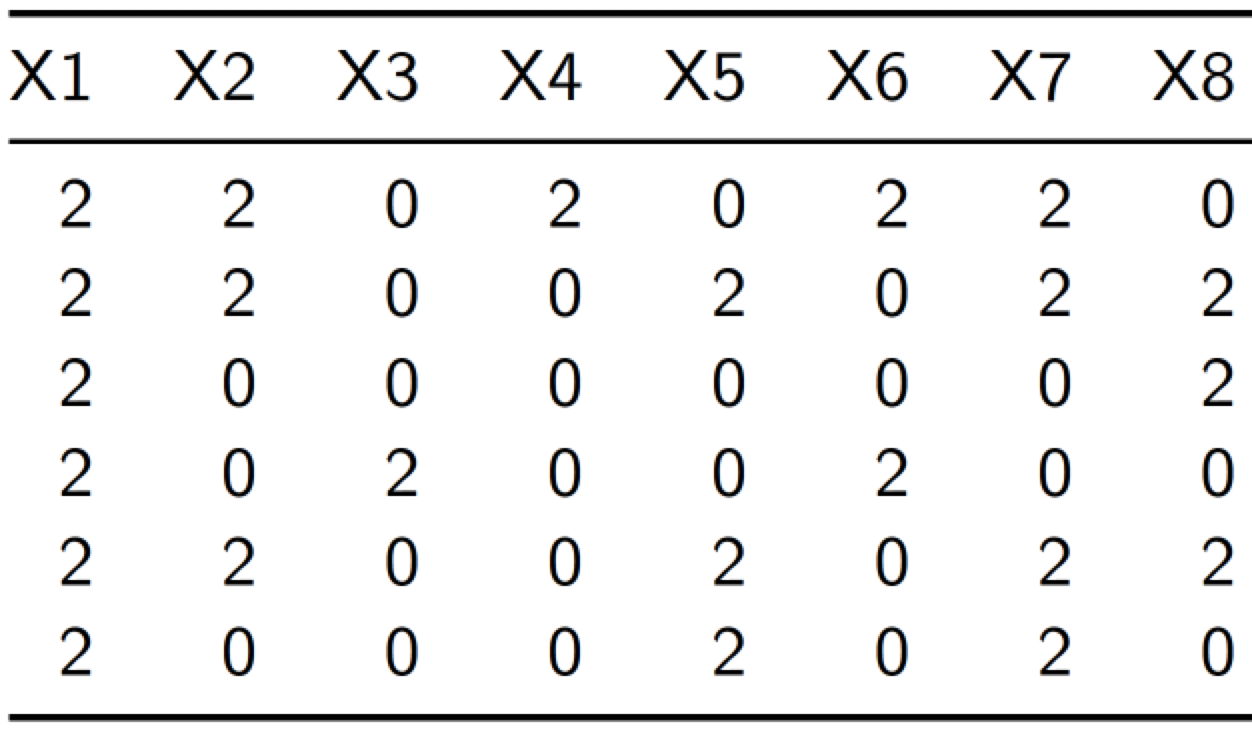
\includegraphics{Pics/21.png}
\caption{\emph{Primeras ocho réplicas del método de las Réplicas Repetidas Balanceadas.}}
\end{figure}

Para la aplicación de la Réplicas Repetidas Balanceadas es recomendable usar el método de Fay, el cual es similar al método Jackknife, pero es más apropiado cuando hay funciones no diferenciables en el estudio. En PISA, por ejemplo, el método de Fay es preferido porque el método Jackknife no proporciona un estimador de varianza estadísticamente consistente para los cuantiles. Por otro lado, la Réplicas Repetidas Balanceadas brinda estimadores lineales simples que son imparciales y consistentes. Además, tiene una consistencia asintótica deseable para un conjunto amplio de estimadores, bajo diseños complejos y estudios de simulación empírica. Bajo la metodología BRR con el ajuste de Fay, el estimador de la varianza toma la siguiente forma:
\[
Var(\hat{\theta}) = \frac{1}{A(1-\rho)^2}\sum_{a=1}^A(\hat{\theta}_a - \hat\theta )^2
\]

En donde \(0<\rho<1\) es el modificador del peso de muestreo de las UPM de la siguiente manera:
\[
d_k^a=
\begin{cases}
\rho*d_k\\ \text{si $k$ no pertenece a la *half-sample*}
(2-\rho)d_k \text{en otro caso}
\end{cases}
\]

Algunos estudios por simulación han mostrado una buena eficiencia para valores de \(\rho\) iguales a 0.3, 0.5 o 0.7.

Para la aplicación de este método, los pesos de muestreo se ajustan para generar los pesos de repetición y, posteriormente, se repiten los ajustes por ausencia de respuesta de escuelas y estudiantes para estos nuevos pesos. Con estos pesos de repetición se estiman los errores de muestreo y la varianza de muestreo, incluyendo el impacto de la ausencia de respuesta, el cual se espera que sea pequeño, pero relevante en el momento de calcular estimadores más precisos.

\begin{figure}
\centering
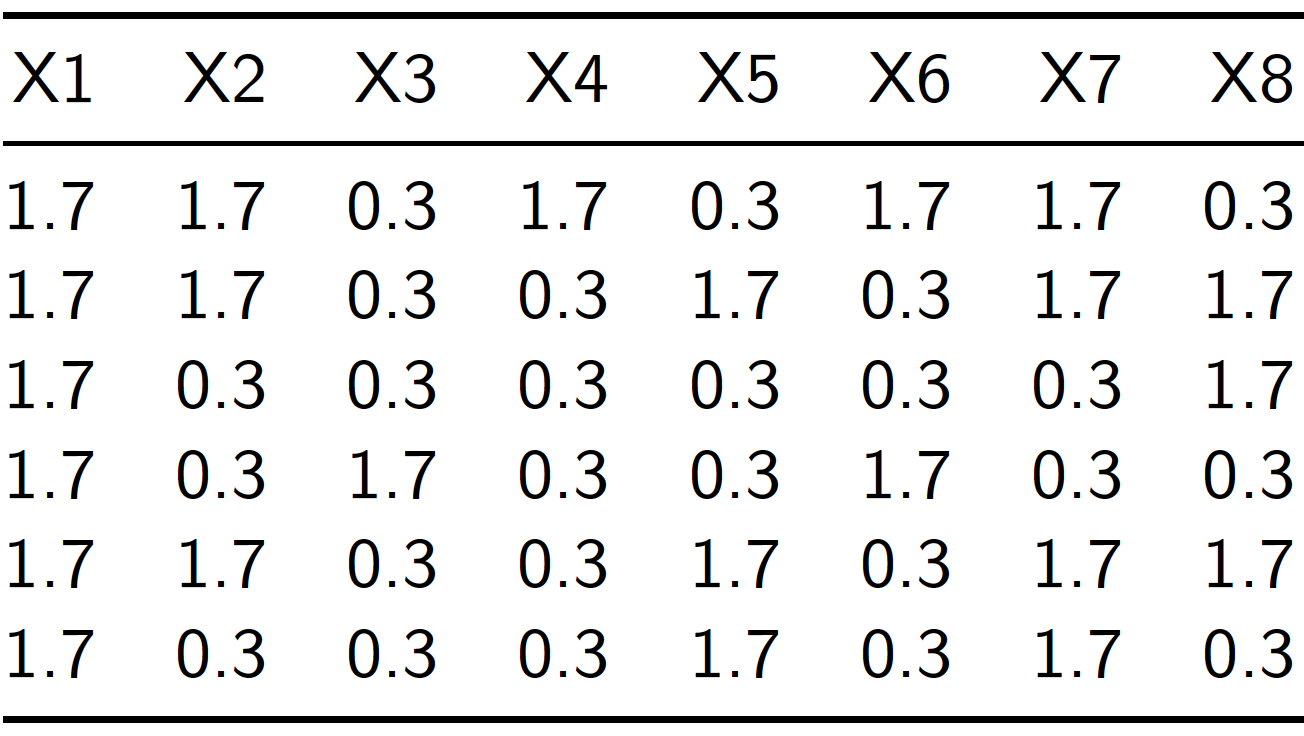
\includegraphics{Pics/22.png}
\caption{\emph{Primeras ocho réplicas del método de las Réplicas Repetidas Balanceadas con el ajuste de Fay.}}
\end{figure}

Para este estudio, si se quiere aplicar esta metodología, debe seguir los siguientes pasos: primero, las unidades de muestreo (escuelas y estudiantes) deben ser agrupadas en los estratos definidos por las tres variables: departamento, sector y zona; segundo, dentro de cada estrato se eliminó una de las unidades (siguiendo una matriz de Hadamard) y se recalcula el peso (peso replicado) para la otra; y tercero, para cada conjunto de pesos replicados se calcula el indicador de interés y se determina su error estándar.

Retomando observaciones hechas anteriormente, hay estratos donde se encuetra solo una escuela, por lo que el método de las réplicas repetidas balanceadas no es aplicable puesto que al eliminar una unidad, algunos estratos quedarán vacíos.

\hypertarget{metodo-de-bootstrap}{%
\subsubsection*{Método de Bootstrap}\label{metodo-de-bootstrap}}
\addcontentsline{toc}{subsubsection}{Método de Bootstrap}

En este apartado se presenta el método de Bootstrap, introducido por Bradley Efron (1979). Este método de remuestreo es el utilizado para este estudio, pues es un método que se implementa fácil, es flexible en términos del número de réplicas que se crean.

Teniendo los pesos muestrales calibrados (denotados por \(w_k^{cal}\)), se procede a crear las réplicas con el método de remuestreo con el fin de poder calcular estimaciones de indicadores junto con las varianzas de estimación. En el contexto de este estudio, se trata de realizar un remuestreo a las unidades primarias de muestreo (escuelas). Se toma a las \(n_I\) escuelas de la muestra como si fuera la población, y de esta población se selecciona una muestra con reemplazo de \(n_I\) selecciones teniendo en cuenta la probabilidad de selección del diseño \(\pi\)-PT de las escuelas. Dado que la selección es con reemplazo, una escuela puede quedar seleccionada más de una vez en esta nueva muestra. Al terminar la selección, se obtiene un vector de tamaño \(n\) (tamaño muestral de los estudiantes) indicando el número de veces que la escuela correspondiente queda seleccionada, posteriormente se multiplica este vector con los pesos muestrales de los estudiantes \(w_k^c\). El anterior proceso se repite un número grande de veces, que para este estudio, se escogió usar 200 réplicas (se usó la función \texttt{as.svrepdesign} de la librería \texttt{survey} para la creación de estas réplicas).

En resumen, para la \(i\)-ésima réplica, se tiene los pesos muestrales \(w_1^i,w_2^i, \cdots, w_n^i\), con \(i=1,\cdots,200\), y estos pesos serán utilizados para calcular las estimaciones de totales, proporciones, promedios y razones y sus respectivas varianzas o desviaciones. Por ejemplo, si para una variable \(y_k\) se requiere estimar el total poblacional \(t_y\), se proce a calcular el total en cada una de las 200 réplicas

\[\hat{t}_y^i=\sum_{k\in s} y_kw_k^i\]
con \(i=1,\cdots,200\). La estimación de \(t_y\) es
\[\hat{t}_y=\frac{1}{200}\sum_{i=1}^{200}\hat{t}_y^i\]
y varianza estimada de la estimación es
\[\hat{Var}(\hat{t}_y)=\frac{1}{199}\sum_{i=1}^{200}(\hat{t}_y^i-\hat{t}_y)^2\]
Usando la anterior expresión de la varianza se puede calcular medidas de precisión para las estimaciones, tales como: coeficiente de variación, margen de error relativo, margen de error absoluto e intervalo de confianza.

\begin{figure}
\centering
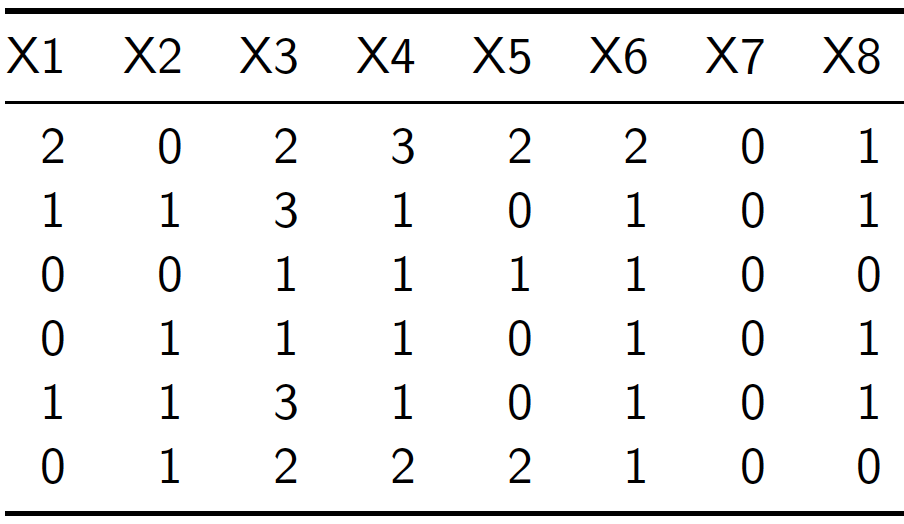
\includegraphics{Pics/23.png}
\caption{\emph{Primeras ocho réplicas del método de Bootstrap.}}
\end{figure}

\hypertarget{error-de-muestreo-utilizando-imputacion-multiple}{%
\subsection*{Error de muestreo utilizando imputación múltiple}\label{error-de-muestreo-utilizando-imputacion-multiple}}
\addcontentsline{toc}{subsection}{Error de muestreo utilizando imputación múltiple}

Por ejemplo, si se quiere realizar mediciones de pobreza utilizando la imputación múltiple es necesario primero establecer un modelo sobre los ingresos \(y_k\) y luego generar \(Q\) posibles valores \(y_k^q \ (q=1, \ldots, Q)\) para cada individuo que no respondió. Luego, utilizando los \(Q\) conjuntos de datos completos, es necesario estimar la siguientes cantidades

\[
\hat{F}_{\alpha}^{q}=\frac{1}{N}\sum_{k\in s} w_k 
\left(\frac{l-y_k}{l}\right)^{\alpha}I(y_k<l) \ \ \ \ \ \ \ \ \ 
q= 1,\ldots, Q.
\]

El estimador final basado en la técnica de imputación múltiple será el promedio simple de las anteriores estimaciones, dado por

\[
\tilde{F}_{\alpha}=\frac{1}{Q}\sum_{q=1}^Q \hat{F}_{\alpha}^{q}
\]

La varianza de esta metodología se puede descomponer en dos componentes, el primero correspondiente a la variación dentro de cada conjunto de datos creado, y el segundo correspondiente a la variación entre cada estimación resultante. Por lo tanto, la varianza asociada a \(\tilde{F}_{\alpha}\) es

\[
\hat{V}(\tilde{F}_{\alpha})
= \frac{1}{Q}\sum_{q=1}^Q \hat{V}(\hat{F}_{\alpha}^{q})
+ \left(1+\frac{1}{Q}\right)\frac{1}{Q-1}\sum_{q=1}^Q (\hat{F}_{\alpha}^{q}-\tilde{F}_{\alpha})^2
\]

Nótese que, una vez se tienen los conjuntos de datos completos, es posible estimar \(\hat{V}(\hat{F}_{\alpha}^{q})\) utilizando las técnicas del último conglomerado en conjunción con el Jackkinfe. Por último, existen otras formas de imputación no probabilística, tales como el vecino más cercano, técnicas de \emph{hot-deck}, imputación lógica, entre otras. En resumen, la característica principal del proceso imputación es utilizar la información auxiliar para aproximar con precisión los valores faltantes. De esta forma, las estimaciones poblacionales de los parámetros de interés tendrán sesgo nulo o despreciable y la confiabilidad de la estrategia de muestreo se mantendrá como se planeó en una primera instancia.

XXXX

\hypertarget{el-efecto-de-diseno-y-el-error-de-muestreo}{%
\section{El efecto de diseño y el error de muestreo}\label{el-efecto-de-diseno-y-el-error-de-muestreo}}

Cuando se selecciona una muestra utilizando un diseño de muestreo complejo es muy improbable que exista independencia entre las observaciones. Una forma sencilla de incorporar el efecto de aglomeración en las expresiones de tamaño de muestra está dada por la siguiente relación, denotada como efecto de diseño \autocite{Kish_1965}:

\[
DEFF=\frac{Var_p(\hat{\theta})}{Var_{MAS}(\hat{\theta})}
\]

En donde \(Var_p(\hat{\theta})\) denota la varianza de un estimador \(\hat{\theta}\) bajo un diseño de muestreo complejo \(p\) y \(Var_{MAS}(\hat{\theta})\) denota la varianza del mismo estimador \(\hat{\theta}\) bajo un diseño de muestreo aleatorio simple \(MAS\). Esta cifra da cuenta del efecto de aglomeración causado por la utilización de un diseño de muestreo complejo \((p)\), frente a un diseño de muestreo aleatorio simple \(MAS\), en la inferencia de un parámetro de la población finita \(\theta\), que puede ser un total, una proporción, una razón, un coeficiente de regresión, etc.

Por ejemplo, suponiendo que el parámetro de interés es la media poblacional (\(\bar{y}_U\)) de una variable de interés \(y\), como el ingreso mensual, es posible escribir la varianza del estimador bajo el diseño de muestreo complejo como

\[
Var_p(\hat{\bar{y}}_U) = \frac{DEFF}{n}\left(1-\frac{n}{N}\right)S^2_{y_U}
\]

En donde \(S^2_{y_U}\) corresponde a la varianza de la características de interés, \(N\) es el tamaño de la población de interés y \(n\) el tamaño de la muestra de individuos. Ahora, al partir de la anterior expresión, es posible mostrar que el tamaño de muestra requerido para estimar este parámetro de interés en una encuesta repetida, con un error de muestreo relativo menor a \(\delta\) y una confianza estadística mayor a \(1-\alpha/2\), está dado por la siguiente expresión.

\[ 
n \geq \dfrac{S^2_{y_U}DEFF}{\dfrac{\delta^2 \bar{y}_U^2}{z_{\alpha}^2}+\dfrac{S^2_{y_U}DEFF}{N}}
\]

En donde \(z_{\alpha}\) es el percentil (\(1- \alpha/2\)) asociado a una distribución normal estándar. Nótese que si \(\rho\) es grande, entonces el valor del efecto de diseño \(DEFF\) también lo será y por consiguiente el tamaño de muestra deberá ser más grande. Por ejemplo, al medir ingresos en la región, debido a la realidad económica de los países, es común encontrar que el tipo de hogar está altamente asociado con el ingreso de los individuos. Esto quiere decir que los ingresos no están uniformemente dispersos a través de todos los hogares, y por ende el coeficiente de correlación intraclase será alto.

Por otro lado, si lo que se quiere estimar es una proporción \(P\), entonces la expresión apropiada para calcular el tamaño de muestra estará dada por

\[ 
n \geq \dfrac{P\ (1-P)\ DEFF}{\dfrac{\delta^2}{z_{\alpha}^2 }+\dfrac{P\ (1-P) \ DEFF}{N}}
\]

La estimación del efecto de diseño es un problema común cuando se trabaja con estimaciones desagregadas en subpoblaciones de interés. Luego, cuando las subpoblaciones constituyen estratos (o agregaciones de estratos) planeados de antemano, para los cuales se conoce previamente su tamaño poblacional, se tiene el siguiente efecto de diseño:

\[
DEFF_h= \frac{Var_p (\hat\theta_h) }{Var_{MAS}^h(\hat\theta_h) }
\]

En donde \(Var_{MAS}^h(\hat\theta_h)\) es la varianza restringida al estrato \(h (h=1,\ldots, H)\), cuyo valor es el siguiente:
\[
Var_{MAS}^h(\hat\theta_h)=\frac{1}{n_h}\left(1-\frac{n_h}{N_h}\right)S_{z_h}^2
\]
Siendo \(n_h\) el tamaño de la muestra en el estrato \(h\), \(N_h\) el tamaño poblacional del estrato \(h\) y \(S_{z_h}^2\) la varianza muestral de la variable linealizada restringida al subgrupo \(h\).

Por otro lado, cuando la subpoblación de interés no es un estrato sino un subgrupo aleatorio - como por ejemplo las personas pobres, las personas menores de 25 años, o cualquier otro subgrupo no planeado en el diseño de la encuesta - cuyo tamaño de muestra es aleatorio entonces la estimación correcta del efecto de diseño es la siguiente:

\[
DEFF_U= \frac{Var_p (\hat\theta_h) }{Var_{MAS}^U(\hat\theta_h) }
\]

En donde \(Var_{MAS}^U(\hat\theta_h)\) es la varianza poblacional del estimador de interés, cuyo valor es el siguiente:

\[
Var_{MAS}^U(\hat\theta_h)=\frac{1}{n}\left(1-\frac{n}{N}\right)S_{z_{hU}}^2
\]

En donde \(S_{z_{hU}}^2\) es la varianza muestral de la variable linealizada calculada en toda la población. Por lo tanto, en ambos efectos de diseño, la estimación de la varianza del diseño de muestreo complejo \(Var_p (\hat\theta_h)\) es la misma, pero el denominador cambia dependiendo de si el subgrupo es un estrato o no. Es por esta razón que en los tres softwares las cifras relacionadas con la estimación puntual, errores estándar, intervalos de confianza y coeficientes de variación coinciden plenamente en los tres softwares.

Ahora, tanto los software Stata como SPSS estiman por defecto el \(DEFF_U\). Nótese que, en este caso, las estimaciones de \(Var_{MAS}^U(\hat\theta_h)\) y \(Var_{MAS}^h(\hat\theta_h)\) serán diferentes, puesto que la primera involucra a toda la muestra, mientras que la segunda involucra únicamente a la muestra del estrato. Retomando el ejemplo, debido a que los subgrupos de interés son agregaciones de los estratos de diseño, no es correcto utilizar el enfoque que Stata trae por defecto.

\hypertarget{agregacion-de-encuestas-y-analisis-longitudinal}{%
\chapter{Agregación de encuestas y análisis longitudinal}\label{agregacion-de-encuestas-y-analisis-longitudinal}}

Para producir indicadores sociales de forma anual, es común recurrir a la agregación de las bases de datos provenientes de las encuestas de hogares, cuya periodicidad puede ser mensual, trimestral o semestral. En este docuemnto se exploran algunas estrategias de estimación ligadas al tratamiento de los pesos inducidos por el diseño de muestreo complejo y al tratamiento de las unidades que se repiten en algún periodo debido al caracter rotativo de la medición.

Uno de los primeros acercamientos al problema de la estimación conjunta de indicadores sociales utilizando varios periodos de recolección se presenta en \textcite{Gurney_Daly_1965}, en donde se examina cómo mejorar el estimador puntual por medio de la correlación natural que se tiene con periodos anteriores, siguiendo un enfoque inferencail basado en modelos estocásticos. \textcite{Lent_Miller_Duff_1999} definen una aproximación a un estimador para las distintas clasificaciones de la fuerza de trabajo que está basado en la optimización de los coeficientes de un estimador compuesto. Por su parte, \textcite{Fuller_1990} provee una discusión acerca de los sesgos que se pueden generar en el análisis de encuestas repetidas debido a errores de medición y revisa detalladamente algunos modelos estimados con mínimos cuadrados. Además, \textcite{Bell_2001} examina varios acercamientos al problema de estimar indicadores sociales, específicamente relacionados con la fuerza de trabajo, provenientes de encuestas de hogares que tienen definido un esquema de rotación y traslape entre distintos periodos de tiempo.

Recientemente, \textcite{Steel_McLaren_2008} revisaron las principales dificualtades al momento de diseñar y analizar encuestas repetidas. Teniendo en cuenta los patrones de rotación en la estimación de los indicadores de nivel y de camnbio, examinan su efecto en la estrategia de estimación de las varianzas de los estimadores de interés. Luego, \textcite{Lewis_2017} definieron algunos procediemientos que se deben seguir al momento de combinar dos o más conjuntos de datos con el propósito de implementar eficicientemente pruebas de significación estadística sobre indicadores de cambio sobre el tiempo, además de incrementar el tamaño de meustra para realizar inferencias de subgrupos poblacionales que están insuficientemente representados en una sola medición.

\hypertarget{esquemas-de-acumulacion-de-muestras}{%
\section{Esquemas de acumulación de muestras}\label{esquemas-de-acumulacion-de-muestras}}

Antes de entrar en los detalles técnicos involucrados en este tipo de procedeimitnos, tomemos una situación ejemplificante específica para ilustrar la problemática que se quiere abordad. Para esto, suponga que una Oficina Nacional de Estadística en América Latina ha previsto una nueva forma de análisis de su encuesta de empleo. Con el fin de tener representatividad a nivel más desagregado (provinicial, por ejemplo), y poder estimar con mayor precisión, ha decidido realizar una agregación anual de todos los levantamientos de su encuesta de empleo. Por ejemplo, suponga que en los meses de marzo, junio, septiembre y diciembre se planean levantamientos trimestrales y que este esquema tenía representatividad nacional, en el área urbana y rural, pero no tenía representatividad provincial, ni de las ciudades principales del país. Con la metodología de agregación de muestras podría ser posible asegurar la representatividad en las provincias desagregadas por área (urbano o rural).

Los procesos de acumulación de muestras son realizados con frecuencia en las encuestas continuas con publicación trimestral. Por ejemplo, se pueden planear levantamientos mensuales y acumular tres meses para realizar la publicación trimestral de la cifra de desempleo. De hecho, algunos países han decidio publicar cifras mensuales del desempleo teniendo en cuenta la acumulación de los úlitmos tres levantamientos, lo que es conocido cono trimiestres móviles. Teniendo en cuenta el diseño rotativo de la mayoría de encuestas en América Latina, una de las bondades de estos esquemas de agregación de muestras en los trimestres móviles es el panel original se mantiene y además, por diseño, la misma vivienda no es entrevistada dos veces en el trimestre movil. En este tipo de diseños, inclusive es posible que, al final de cada año en diciembre, se contemple la publicación de un gran agregado anual que contemple la agregación de los doce meses anteriores. En este escenario sí existen viviendas que han sido entrevistadas dos veces y este porcentaje, dependiendo del diseño rotativo, puese no ser bajo. Por ejemplo, en un panel 2(2)2, el diseño rotativo induce un traslape natural del 50\% entre trimestres.

\textcite[capítulos 7 y 8]{Korn_Graubard_1999} proveen un recuento exhaustivo sobre las opciones de ponderación y otros temas a considerar cuando se combinan datos a lo largo del tiempo en encuestas complejas. En el caso de la agregación de muestras se resalta que todas las viviendas que han sido entrevistadas en más de una ocasión deben pertenecer a la misma UPM por diseño. Es muy importante que la identificación de las UPMs y de los estratos de muestreo se debe realizar de manera inequívoca y se debe asegurar que los siguientes principios se cumplas a cabalidad:

\begin{quote}
\emph{1. Cuando se combinan dos o más oleadas del mismo panel es importante asegurarse que las UPMs sean emparejadas correctamente, de tal forma que el software las reconozca como iguales.}
\end{quote}

\begin{quote}
\emph{2. Cuando se combinan dos o más muestras independientes es importante asegurarse que las UPMs estén codificada de tal forma que el software las reconozca como distintas.}
\end{quote}

Cuando se trata de estimar las varianzas de este tipo de estimadores, los cálculos analíticos se tornan mucho más complicados. \textcite{Train_Cahoon_Makens_1978} muestran lo complicado que puede ser calcular las variaciones de los promedios de las estimaciones de múltiples períodos de tiempo en una encuesta repetida y cómo estos cálculos dependen en gran manera del patrón de traslape definido en el diseño de la encuesta. Para las encuestas de población activa, a menudo se utiliza un enfoque computacional basado en métodos de remuestreo, como \emph{Jackknife}, \emph{Bootstrap} o \emph{BRR}. Nótese que el uso apropiado de tales métodos, también dependerá del origen de la encuesta y de sus objetivos. Por ejemplo, los insumos de aplicación de los métodos serían unos si la encuesta está orientada a medir el desempleo (por ejemplo, porque es una encuesta nacional de la fuerza de trabajo llevada a cabo por un instituto nacional de estadística), y serían diferentes si la encuesta está diseñada para estimar los cambios brutos entre dos periodos de tiempo.

Actualmente, los softwares estadísticos más comunmente utilizados incluyen procedimientos para la estimación de la varianza teniendo en cuenta diseños de muestreo complejos. Una forma sencilla de usarlos es siguiendo estos pasos:

\begin{enumerate}
\def\labelenumi{\arabic{enumi}.}
\tightlist
\item
  Modificar los pesos, de tal forma que cumplan las restricciones poblacionales básicas.
\item
  Definir los estratos de interés en donde el diseño de meustreo se realiza de forma independiente.
\item
  Definir estrictamente las UPM como aglomerados poblacionales que incluyen a los hogares y personas (con sus múltiples entrevistas).
\item
  Realizar una estimación de la razón entre el número de personas desempleadas, como el numerador, y el núemro de personas que pertenecen a la fuerza de trabajo, como el denominador.
\end{enumerate}

Suponiendo una muestra grande, la varianza resultante, calculada de esta manera, será un poco conservadora (sobreestimada).

\hypertarget{factores-de-expansion-y-estimadores-de-muestreo}{%
\section{Factores de expansión y estimadores de muestreo}\label{factores-de-expansion-y-estimadores-de-muestreo}}

Si el investigador está interesado en estimar la tasa de desempleo anual de una encuesta rotativa, que se lleva a cabo cuatro veces al año, es posible usar los cuatro conjuntos de datos y unir los cuatro trimestres para estimar la tasa de desempleo anual. Una solución inicial a este problema consiste en unir los cuatro conjuntos de datos y dividir los pesos de muestreo de cada periodo por un factor de cuatro. El anterior procedimiento induce estimadores puntuales aproximadamente insesgados, aunque las estimaciones de los errores estándar se tornan un poco más complicadas, puesto que se debe concatenar exahustivamente las UPM (o incluso crear algunas pseudo-UPM), si el archivo no contiene códigos de grupo.

Por supuesto, las encuestas que utilizan diseños rotativos, en donde un hogar es entrevistado en varias ocasiones, deben adjuntar dos clases de pesos de muestreo: los transversales y los longitudinales. Los pesos transversales, discutidos en las secciones anteriores, son aquellos inducidos por el diseño de muestreo de la encuesta en cada aplicación y que permiten obtener estimaciones de los parámetros de interés de forma periódica (mensual, trimestral o semestral). De esta forma, por ejemplo en una encuesta de fuerza de trabjo, los datos transversales se usarán para producir estimaciones periódicas de la participación en la fuerza de trabajo, o de la tasa de pobreza, o de la tasa de desempleo, de manera periódica. Por ejemplo, la estimación de la tasa de desempleo usa un promedio ponderado de la siguiente forma

\[\hat\theta=\frac{\sum_s w_ky_k}{\sum_s w_kz_k}\]

En donde, para la persona \(k\)-ésima, \(w_k\) representa su peso de muestreo, \(y_k\) representa su estado de ocupación (específicamente, \(y_k=1\) si la persona está desempleada) y \(z_k\) es su estado en la fuerza de trabajo (específicamente, \(z_k=1\) si la persona pertenece a la fuerza de trabajo). Esta estrategia de estimación asume que cada persona se representa a sí misma y a otras más en la población. Nótese que los pesos transversales asignados estarán determinados por la probabilidad de selección de las UPMs, la probabilidad de selección del hogar dentro de la UPMs, el ajuste por ausencia de respuesta en ese mismo mes, ajustes de submuestreo, calibración, entre otros. Por tales razones, aunadas a la incorporación de la nueva muestra en un diseño rotativo, además de la ausencia de respuesta y también por los cambios en el tamaño de la población de interés, el peso de un individuo puede cambiar de un periodo a otro. De esta forma, si \(w_k^{t-1}\) y \(w_k^{t}\) representan el peso de muestreo del individuo \(k\) en los periodos \(t-1\) y \(t\), respectivamente, es casi seguro que

\[w_k^{t-1} \neq w_k^t\]

Es posible considerar diferentes acercamientos ante esta situación. \textcite{Feinberg_Stasny_1983} asumen que las diferencias en los dos pesos ocurren solamente como resultado de los flujos naturales de entrada y salida de la población de interés. Por ejemplo, si el individuo es clasificado como empleado en ambos tiempos y \(w_k^{t-1}=300\) y \(w_k^{t}=305\), entonces el peso mínimo, 300, se añade a la celda (Empleado - Empleado) de la tabla de cambios brutos y la diferencia entre los pesos, 5, se añade a la celda (Fuera - Empleado). Si por el contrario, \(w_k^{t-1}=305\) y \(w_k^{t}=300\), entonces el peso mínimo, 300, se añade a la celda (Empleado - Empleado) de la tabla de cambios brutos y la diferencia entre los pesos, 5, se añade a la celda (Empleado - Fuera). Este enfoque supone que las diferencias entre los pesos están supeditadas a las fluctuaciones que se puedan presentar en la fuerza de trabajo. Aunque es posible considerar otros supuestos, en cualquier caso es necesario crear un nuevo conjunto de pesos (llamados pesos longitudinales) que resulten del traslape de las bases de datos en los tiempos \(t-1\) y \(t\). Por ejemplo, siguiendo la metodología de la encuesta \emph{Survey of Labour and Income Dynamics} \autocites{Naud_2002}{LaRoche_2003}, estos pesos pueden ser ajustados por un factor \(\gamma\) (que resulta ser el inverso de la probabilidad de traslape). De esta forma un primer paso para crear los pesos longitudinales es mediante la siguiente expresión

\[w_k^{longitudinal} = \gamma \  w_k^{t}\]

En conjunción con lo anterior y teniendo en cuenta que es posible que los INE ya hayan publicado las cifras oficiales del parámetros de interés en los tiempos \(t-1\) y \(t\), es necesario que los totales fila coincidan con las estimaciones publicadas en el periodo \(t-1\) y que los totales columna coincidan con las estimaciones publicadas en el periodo \(t\). Para mantener esta consistencia es posible utilizar el método de \emph{Raking} que se incializa con un factor de expansión inicial para el análisis de los trimestres móviles que debe ser modificado de manera proporcional a los pesos originales de los levantamientos mensuales teniendo en cuenta la siguiente relación

\[
\hat{t}_y = \sum_{s1 \cup s2 \cup s3} w_k y_k
= \sum_{s1} d_{1k} y_k + \sum_{s2} d_{2k} y_k + \sum_{s3} d_{3k} y_k
\]

Por lo tanto, en la agregación trimestral el factor de expansión de cada individuo y hogar debe ser multiplicado por el siguiente factor:

\[
a_i = \frac{\sum_{k\in s_i}d_{ik}}{\sum_{i=1}^{3}\sum_{k\in s_i}d_{ik}}
\]

El factor de expansión para el análisis de la agregación anual debe ser modificado de manera proporcional a los pesos originales de los levantamientos mensuales y trimestrales teniendo en cuenta la siguiente relación

\[
\hat{t}_y = \sum_{s_1 \cup ... \cup s_{12}} w_k y_k
= \sum_{s_1} d_{1k} y_k + \cdots + \sum_{s_{12}} d_{12k} y_k
\]

Por lo tanto, en la agregación anual el factor de expansión de cada individuo y hogar debe ser multiplicado por el siguiente factor:

\[
b_i = \frac{\sum_{k\in s_i}d_{ik}}{\sum_{i=1}^{12}\sum_{k\in s_i}d_{ik}}
\]

La nueva estructura longitudinal de los pesos debe garantizar que la la suma de los pesos esté acorde con la población a la cual quiere representar.

\[
\sum_{i}^{3}\sum_{s_i} a_i d_{ik} \approx N
\]

\[
\sum_{i}^{12}\sum_{s_i} b_i d_{ik} \approx N
\]

Una vez se han construido los pesos longitudinales, es necesario realizar los siguientes chequeos para verificar que la ponderación es correcta:

\begin{itemize}
\tightlist
\item
  Suma de pesos en las cinco ciudades
\item
  Suma de pesos a nivel nacional
\item
  Suma de pesos por rural/urbano
\item
  Suma de pesos en cada una de las provincias (en el caso de la agregación anual)
\end{itemize}

Una vez que se haya generado la base de datos agregada (trimestral o anual) es necesario decidir acerca de qué totales auxiliares serán utilizados en esta calibración. Por ejemplo en la agregación trimestral, es posible escoger el mes intermedio o el promedio de los tres meses. Se espera que este ajuste final de los pesos sea minúsculo y no afecte la estructura de los pesos mensuales puesto que se trata de calibrar unos pesos que orignalmente fueron calibrados en las publicaciones mensuales. Por otro lado, debido a que este último paso se realiza con propósitos de mantener la consistencia de las publicaciones, es posible que la calibración se vea reducida al considerar menos restricciones sobre los totales auxiliares más relevantes.

Se recalca que las agregaciones deberían contemplar a todas las viviendas que fueron parte del trimestre móvil. Mientras que las agregaciones anuales deben contemplar las viviendas que han sido seleccionadas más de una vez (debido al esquema de rotación del panel) y por ende todas sus mediciones deben aparecer en la base de datos tantas veces como fueron visitadas. Por otro lado, las agregaciones trimestrales no deberían contemplar ninguna vivienda con mediciones repetidas puestos que el esquema de panel actual no lo contempla. Nótese que es necesario realizar el correspondiente ajuste a los pesos de muestreo sin diferenciar si la vivienda apareció una vez o fue medida en más de una ocasión.

En la estimación del error de muestreo para las agregaciones trimestrales se debe considerar que el muestreo es independiente en los tres meses que componen el trimestre móvil y por ende la posibilidad de tener viviendas repetidas es muy cercana a cero. Nótese que el estimador de interés toma la siguiente forma:

\[
\hat{t}_y 
= \sum_{s1} d_{1k} y_k + \sum_{s2} d_{2k} y_k + \sum_{s3} d_{3k} y_k
= \hat{t}_{y}^1 + \hat{t}_{y}^2 + \hat{t}_{y}^3
\]
En este caso, la varianza del estimador está dada por

\[
Var(\hat{t}_y)
= Var(\hat{t}_{y}^1) + Var(\hat{t}_{y}^2) + Var(\hat{t}_{y}^3)
\]

En la estimación del error de muestreo para las agregaciones anuales se debe considerar que el muestreo no es independiente en los doce meses. Nótese que el estimador de interés toma la siguiente forma:

\[
\hat{t}_y 
= \sum_{i=1}^{12}\sum_{s_i} d_{ik} y_k 
= \sum_{i=1}^{12} \hat{t}_{y}^i
\]

En este caso, la varianza del estimador está dada por

\[
Var(\hat{t}_y) 
= \sum_{i=1}^{12} Var(\hat{t}_{y}^i)
+ 2 \sum_{i=1}^{12} \sum_{j < i} Cov(\hat{t}_{y}^i, \hat{t}_{y}^j)
\]

Una vez que se ha llevado a cabo el proceso de computo de los nuevos pesos longitudinales en las agregaciones (trimestrales o anuales) es necesario que se realice nuevamente un proceso de calibración sobre las variables involucradas en la calibración mensual.

\hypertarget{efecto-del-tipo-de-encuesta-en-la-eficiencia-de-los-indicadores}{%
\section{Efecto del tipo de encuesta en la eficiencia de los indicadores}\label{efecto-del-tipo-de-encuesta-en-la-eficiencia-de-los-indicadores}}

Lograr una estimación adecuada del error de muestreo en las comparaciones de múltiples periodos de tiempo, ya sea con la agregación de datos o no, debe ser una de las principales tareas del investigador. Además, dependiendo del parámetro, la naturaleza del error de muestreo cambia así como el tamaño de muestra requerido para satisfacer las necesidades de precisión de las estimaciones.

\hypertarget{cambios-netos}{%
\subsection*{Cambios netos}\label{cambios-netos}}
\addcontentsline{toc}{subsection}{Cambios netos}

Por ejemplo, considere el cambio neto de la media de la variable de interés \(x\) en dos periodos de tiempo (\(t_2\) y \(t_1\))

\[
\Delta = \bar{x}_2 - \bar{x}_1
\]

Este parámetro de cambio en los dos periodos de tiempo es estimado de forma aproximadamente insesgada mediante la siguiente expresión:

\[
\hat{\Delta} = \hat{\bar{x}}_2 - \hat{\bar{x}}_1
= \frac{\sum_{k\in s_2}\frac{x_{k}}{\pi_k}}{\sum_{k\in s_2}\frac{1}{\pi_k}} - \frac{\sum_{k\in s_1}\frac{x_{k}}{\pi_k}}{\sum_{k\in s_1}\frac{1}{\pi_k}} 
\]

En donde \(s_2\) y \(s_1\) representan las muestras seleccionadas en los periodos de interés y \(\pi_k\) es la probabilidad de inclusión del elemento \(k\). La varianza del estimador de cambio se calcula mediante la siguiente expresión:

\[
Var(\hat{\Delta}) = Var(\hat{\bar{x}}_2) + Var(\hat{\bar{x}}_1) - 2Cov(\hat{\bar{x}}_2, \hat{\bar{x}}_1)
\]

En general, el último término se puede expresar como

\[
2Cov(\hat{\bar{x}}_2, \hat{\bar{x}}_1) = 
2\sqrt{Var(\hat{\bar{x}}_2)}\sqrt{Var(\hat{\bar{x}}_1)}\sqrt{T_2}\sqrt{T_1}R_{12}
\]

En donde \(T_2\) y \(T_1\) representan el porcentaje de muestra común que se traslapa en ambos levantamientos y \(R_{12}\) representa la correlación de la variable de interés \(x\) en los periodos observados. Suponiendo que la variación de la variable de interés es homogénea en ambos periodos y que el traslape es común por diseño, entonces la expresión de la varianza se reduce de la siguiente manera:

\[
Var(\hat{\Delta}) = 2Var(\hat{\bar{x}}) - 2\sqrt{Var(\hat{\bar{x}})}TR
=2Var(\hat{\bar{x}})(1-TR) 
\]

Nótese que la varianza de este indicador cambiará de acuerdo al tipo de encuesta que se elija:

\begin{itemize}
\tightlist
\item
  Encuesta repetida: en donde \(T=0\) y
  \[Var(\hat{\Delta}) = 2Var(\hat{\bar{x}})\].
\item
  Encuesta de panel, en donde \(T=1\), \(R > 0\) y
  \[Var(\hat{\Delta}) = 2Var(\hat{\bar{x}})(1-R)\].
\item
  Encuesta rotativa: en donde \(T\neq 0\), \(R > 0\) y
  \[Var(\hat{\Delta}) = 2Var(\hat{\bar{x}})(1-TR)\].
\end{itemize}

Si se supone que la \textbf{correlación es positiva} para la variable en los dos periodos de tiempo, entonces se tiene la siguientes conclusión:

\[
2Var(\hat{\bar{x}})(1-R) < 2Var(\hat{\bar{x}})(1-TR) < 2Var(\hat{\bar{x}})
\]

Es decir que se necesita \textbf{menos} tamaño de muestra para medir los cambios netos usando un diseño panel que un diseño sin traslape. Un camino medio es el diseño rotativo.

\hypertarget{promedio-trimestral}{%
\subsection*{Promedio trimestral}\label{promedio-trimestral}}
\addcontentsline{toc}{subsection}{Promedio trimestral}

Considere una encuesta continua y mensual en donde se quiere estimar el promedio trimestral de la variable de interés \(x\) en tres periodos de tiempo (\(t_3\), \(t_2\) y \(t_1\))

\[
\Theta = \frac{\bar{x}_3 + \bar{x}_2 + \bar{x}_1}{3}
\]

Un estimador del promedio trimestral que es estimado de forma aproximadamente insesgada mediante la siguiente expresión:

\[
\hat{\Theta} = \frac{1}{3} \left( \hat{\bar{x}}_3 + \hat{\bar{x}}_2 + \hat{\bar{x}}_1 \right)
= \frac{1}{3}\left( \frac{\sum_{k\in s_3}\frac{x_{k}}{\pi_k}}{\sum_{k\in s_3}\frac{1}{\pi_k}} + \frac{\sum_{k\in s_2}\frac{x_{k}}{\pi_k}}{\sum_{k\in s_2}\frac{1}{\pi_k}} + \frac{\sum_{k\in s_1}\frac{x_{k}}{\pi_k}}{\sum_{k\in s_1}\frac{1}{\pi_k}} \right)
\]

En donde \(s_3\), \(s_2\) y \(s_1\) representan las muestras seleccionadas en los periodos de interés y \(\pi_k\) es la probabilidad de inclusión del elemento \(k\). La varianza del estimador del promedio trimestral se calcula mediante la siguiente expresión:

\[
\begin{split}
Var(\hat{\Theta}) & = \frac{1}{9}[Var(\hat{\bar{x}}_3) + Var(\hat{\bar{x}}_2) + Var(\hat{\bar{x}}_2) + \\ 
&2Cov(\hat{\bar{x}}_3, \hat{\bar{x}}_2)) + 2Cov(\hat{\bar{x}}_3, \hat{\bar{x}}_1)) + 2Cov(\hat{\bar{x}}_2, \hat{\bar{x}}_1)]
\end{split}
\]

Suponiendo que la variación de la variable de interés es homogénea en ambos periodos y que el traslape es común por diseño y que los errores de muestreo son débilmente estacionarios entre dos y tres meses, entonces la expresión de la varianza se reduce de la siguiente manera:

\[
Var(\hat{\Theta}) = \frac{1}{9} Var(\hat{\bar{x}})[3 + 6TR]
\]

En donde \(R\) es la correlación de la variable de interés en dos y tres meses (asumida homogénea). Nótese que la varianza de este indicador cambiará de acuerdo al tipo de encuesta que se elija:

\begin{itemize}
\tightlist
\item
  Encuesta repetida: en donde \(T=0\) y
  \[Var(\hat{\Theta}) = \frac{1}{3} Var(\hat{\bar{x}})\].
\item
  Encuesta de panel, en donde \(T=1\), \(R > 0\) y
  \[Var(\hat{\Theta}) = \frac{1}{3} Var(\hat{\bar{x}}) [3+6R]\].
\item
  Encuesta rotativa: en donde \(T\neq 0\), \(R > 0\) y
  \[Var(\hat{\Theta}) = \frac{1}{3} Var(\hat{\bar{x}}) [3+6TR]\].
\end{itemize}

De esta forma, si se supone que la \textbf{correlación es positiva} para la variable en los tres periodos de tiempo, entonces se tiene la siguiente conclusión:

\[
\frac{1}{3} Var(\hat{\bar{x}}) [3+6R] > \frac{1}{3} Var(\hat{\bar{x}}) [3+6TR] > \frac{1}{3} Var(\hat{\bar{x}})
\]

Es decir que se necesita \textbf{más} tamaño de muestra para estimar un promedio trimestral usando un diseño panel que un diseño sin traslape.

\hypertarget{pruebas-de-hipotesis-sobre-indicadores-longitudinales}{%
\section{Pruebas de hipótesis sobre indicadores longitudinales}\label{pruebas-de-hipotesis-sobre-indicadores-longitudinales}}

Para decidir si un cambio en la dinámica de los parámetros de interés es significativo entre dos periodos de tiempo es necesario llevar a cabo una prueba de hipóstesis. Por ejemplo, tomando en cuenta la dinámica del mercado de trabajo, es posible realizar comparaciones entre dos trimestres seguidos o entre dos años consecutivos para conocer, por ejemplo, si hay un cambio significativo e importante en la reducción de la desocupación (entre grupos y en distintos periodos del tiempo).

Para realizar comparaciones entre grupos de un mismo corte transversal (por ejemplo comparar la situación laboral de hombres y mujeres en un mes específico) es necesario tener en cuenta que el muestreo de la primera etapa es de UPMs y que el tamaño de muestra de hombres y mujeres es aleatorio. Para realizar comparaciones nacionales o regionales en dos periodos de tiempo (por ejemplo comparar la situación laboral de un paíse entre dos trimestres) es necesario tener en cuenta que el muestreo puede no ser independiente entre trimestres ni entre años, siendo este el caso de las enceustas que contemplan diseños de panel rotativo. Considere el siguiente sistema de hipótesis:

\[
H_0: \theta_2 - \theta_1 = 0 \ \ \ \ vs. \ \ \ \ H_1: \theta_2 - \theta_1 \neq 0
\]

Para llevar a cabo la prueba de hipótesis trabajamos con el siguiente estimador de diferencias:

\[
\hat{d} = \hat{\theta}_2 - \hat{\theta}_1
\]

La varianza asociada a este estimador está dada por

\[
Var(\hat{d}) 
= Var(\hat{\theta}_2) + Var(\hat{\theta}_1) - 2 Cov(\hat{\theta}_1, \hat{\theta}_2) 
\]

Y por último, el término de covarianza se puede escribir como

\[
Cov(\hat{\theta}_1, \hat{\theta}_2) = \sqrt{Var(\hat{\theta}_1)}\sqrt{Var(\hat{\theta}_2)}\sqrt{P_1}\sqrt{P_2}R_{1,2}
\]

Existen muchos escenarios de comparación que son de interés cuando se analizan datos de una encuesta de empleo. Estas comparaciones se hacen mas complejas cuando se incluye en el análisis el diseño en panel de la encuesta. Sin embargo, cuando se cumple el siguiente principio no habrá lugar a confusión

\begin{quote}
\emph{A no ser que los dos estimadores puntuales estén compuestos de observaciones provenientes de un conjunto disyunto de UPMs, el término de covarianza no será nulo.}
\end{quote}

\hypertarget{ejemplos}{%
\subsection{Ejemplos}\label{ejemplos}}

\hypertarget{covarianza-en-comparaciones-mensuales}{%
\subsubsection*{Covarianza en comparaciones mensuales}\label{covarianza-en-comparaciones-mensuales}}
\addcontentsline{toc}{subsubsection}{Covarianza en comparaciones mensuales}

Suponga que se quiere comparar la tasa de desempleo nacional entre dos meses consecutivos. En este escenario existe independencia en el muestreo de los dos meses consecutivos y por lo tanto el porcentaje de traslape de muestra entre los dos meses (que por diseño es nulo) es igual a cero.

Por lo tanto, \(P_1 = P_2 = 0\). Luego, el término de la covarianza se anula. En resumen, la varianza del estimador en este caso sería igual a:

\[
Var(\hat{d}) 
= Var(\hat{\theta}_2) + Var(\hat{\theta}_1)
\]

\hypertarget{covarianza-en-comparaciones-trimestrales-o-anuales}{%
\subsubsection*{Covarianza en comparaciones trimestrales o anuales}\label{covarianza-en-comparaciones-trimestrales-o-anuales}}
\addcontentsline{toc}{subsubsection}{Covarianza en comparaciones trimestrales o anuales}

Suponga que se quiere comparar la tasa de desempleo nacional entre trimestres consecutivos o entre el mismo mes de dos años consecutivos. En este escenario no existe independencia en el muestreo de los dos trimestres consecutivos puestos que la estructura del panel garantiza un traslape del 50\%. En este caso \(P_1 = P_2 \approx 0.5\).

Por otro lado, existe una correlación natural entre las viviendas comunes en el panel que se midieron en los periodos de interés, por lo tanto \(R_{1,2} \neq 0\). Note que esta correlación se calcula sobre los individuos comunes en el panel y sobre la variable dicotómica que induce la tasa de desempleo (perteneciente a la fuerza de trabajo + estado de ocupación).

En resumen, el término de covarianza en este caso sería igual a:

\[
Cov(\hat{\theta}_1, \hat{\theta}_2) = \frac{1}{2}\sqrt{Var(\hat{\theta}_1)}\sqrt{Var(\hat{\theta}_2)}R_{1,2}
\]

\hypertarget{covarianza-en-comparaciones-de-un-mismo-mes}{%
\subsubsection*{Covarianza en comparaciones de un mismo mes}\label{covarianza-en-comparaciones-de-un-mismo-mes}}
\addcontentsline{toc}{subsubsection}{Covarianza en comparaciones de un mismo mes}

Suponga que se quiere comparar la tasa de desempleo entre hombres y mujeres en un mismo mes. A pesar de que la estructura de panel no se considere, en este escenario no existe independencia en el muestreo de hombres y mujeres puesto que estos grupos no son estratos de muestreo. En este caso \(P_1\) es la proporción de hombres en la muestra y \(P_2\) es la proporción de mujeres en la muestra. Nótese que \(P_1 \neq P_2\).

Por otro lado, existe una correlación natural entre las UPMs que fueron seleccionadas y que contienen tanto a hombres como a mujeres, por lo tanto \(R_{12} \neq 0\). Note que esta correlación se calcula sobre todos los individuos de la muestra pertenecientes a la fuerza de trabajo y sobre la variable dicotómica que induce la tasa de desempleo. En resumen, el término de covarianza en este caso sería igual a:

\[
Cov(\hat{\theta}_1, \hat{\theta}_2) = \sqrt{Var(\hat{\theta}_1)}\sqrt{Var(\hat{\theta}_2)}\sqrt{P_1}\sqrt{P_2}R_{1,2}
\]

\hypertarget{covarianza-en-comparaciones-de-un-mismo-mes-1}{%
\subsubsection*{Covarianza en comparaciones de un mismo mes}\label{covarianza-en-comparaciones-de-un-mismo-mes-1}}
\addcontentsline{toc}{subsubsection}{Covarianza en comparaciones de un mismo mes}

Suponga que se quiere comparar la tasa de desempleo entre Quito y Guayaquil en un mismo mes. En este escenario existe independencia en el muestreo de las dos ciudades porque la selección es independiente en cada ciudad. Esta independencia se tiene por definición del diseño de muestreo puesto que ambas ciudades son estratos de muestreo. En este caso \(P_1\) es la proporción de personas de Quito en la muestra y \(P_2\) es la proporción de personas de Guayaquil en la muestra. Nótese que \(P_1 \neq P_2\).

Por otro lado, no existe una correlación entre las UPMs que fueron seleccionadas en Quito y Guayaquil porque la selección fue independiente, por lo tanto \(R_{12} = 0\). En resumen, el término de covarianza es nulo y por ende la varianza del estimador sería igual a:

\[
Var(\hat{d}) 
= Var(\hat{\theta}_2) + Var(\hat{\theta}_1)
\]

\hypertarget{estadistico-de-prueba}{%
\subsection{Estadístico de prueba}\label{estadistico-de-prueba}}

Una vez se ha definido la estructura de varianza del estimador de interés, el siguiente paso es definir si la siguiente cantidad es distinta de cero para determinar si el parámetro ha cambiado entre grupos o a lo largo del tiempo.

\[
t = \frac{\hat{d}}{\sqrt{Var(\hat{d})}}
\]

Este estadístico de prueba sigue una distribución \emph{t-student} con \(df\) grados de libertad que están dados por la resta entre el número de UPMs seleccionadas menos el número de estratos de muestreo considerados. De esta forma, se tiene que:

\[
df = \sum_{h=1}^H (n_{Ih} - 1) = \sum_{h=1}^H n_{Ih} - H = \#UPMs - \#Estratos
\]

Los grados de libertad permiten tener una inferencia precisa a medida que crecen. Por ejemplo, considere por ejemplo el percentil 0.975 para el cual los valores críticos de la distribución varían con respecto a sus grados de libertad: \(t_{0.975, 1}=12.7\), \(t_{0.975, 20}=2.08\), \(t_{0.975, 40}=2.02\), \(t_{0.975, \infty}=1.96\). Los grados de libertad son determinantes a la hora de hacer inferencias dentro de subpoblaciones de interés. En este caso los grados de libertad no se consideran fijos sino variables. \textcite{Korn_Graubard_1999} proponen el siguiente método de cálculo sobre los grados de libertad en subpoblaciones:

\[
df_{subpoblación} = \sum_{h=1}^H v_h(n_{Ih} - 1)
\]

En donde \(v_h\) es una variable indicadora que toma el valor uno si el estrato \(h\) contiene uno o mas casos de las subpoblaciones de interés y toma el valor cero en otro caso.

\hypertarget{criterios-de-calidad}{%
\chapter{Criterios de calidad}\label{criterios-de-calidad}}

Los equipos encargados del muestreo en las Oficinas Nacinoales de Estadística (ONEs) en Latinoamérica y el Caribe han adelantado un extenso trabajo en cuanto a los criterios de supresión de cifras para determinar si una estadística debe ser considerada como precisa y confiable en cuanto a su utilización para la toma de decisiones de política pública. El trabajo de socialización interna con los diferentes analistas de la infomración ha sido riguroso y debe continuar en la misma dirección apropiada hasta lograr interiorizar en las ONEs una visión más exhaustiva y amplia en cuanto a la confiabilidad de una cifra resultante de la encuesta.

En este contexto, mucho se ha discutido acerca del uso del coeficiente de varaición en la validación de la confiabilidad y precisión de las cifras que provienen de estudios por muestreo. Se realizó una revisión de las experiencias internacionales, para determinar si a nivel internacional se usan criterios de supresión de información y los umbrales que los Institutos Nacionales de Estadística utilizan para la validación de las cifras, tanto en encuestas de hogares como en encuestas de negocios. A continuación se muestra el resumen de lo encontrado.

\begin{quote}
\emph{En encuentas de hogares, se encontró que Sudáfrica utiliza el umbral del 35\% sobre el coeficiente de variación, Estado Unidos y los países del Mercosur utilizan un umbral del 30\%, Australia, Canadá y México usan como referencia un umbral del 25\%, Chile, Costa Rica, Eslovaquia, Holanda, Islandia y Portugal utilizan un umbrla del 20\%, Ecuador y Perú utilizan un umbral del 15\%, Alemania, Colombia, Eslovenia y Suiza utilizan un umbral del 10\%. De esta forma, cualquier cifra estimada cuyo coeficiente de variación sea mayor al umbral predefinido será suprimida o marcada como una cifra poco confiable.}
\end{quote}

Sarndal et. al. (2003) expresa que ``un estadístico puede expresar su opinión de que un valor del coeficiente de variación del 2\% es bueno, considerando las restricciones de la encuesta, mientras que un valor del coeficiente de variación de 9\% puede ser considerado inaceptable''. Cuando se sobrepasa el umbral del coeficiente de variación algunas ONE publican las cifras y junta a ellas algunas alertas, como las siguientes:

\begin{itemize}
\tightlist
\item
  No se publica
\item
  Usar con precaución.
\item
  Los coeficientes de variación mayores a 20, significan que los ingresos estimados están sujetos a una alta variabilidad, lo que limita su alcance para fines analíticos.
\item
  Las estimaciones requieren revisiones, no son precisas y se deben usar con precaución.
\item
  Poco confiable, menos preciso. Se usa la letra M o () para que se use con cuidado.
\item
  Con reserva, referencial, cuestionable.
\item
  Valores muy aleatorios, estimación pobre.
\end{itemize}

Una encuesta se planea con el fin de generar información precisa y confiable en los dominios de estudio que se han predefinido. Sin embargo, existen subgrupos poblacionales que la encuesta no abordó en su diseño, y sobre los cuales se quisiera una mayor precisión.

\begin{itemize}
\tightlist
\item
  Incidencia de la pobreza desagregado por departamento o provincia (tamaño de muestra conocido y planificado).
\item
  Tasa de desocupación desagregada por sexo (tamaño de muestra aleatorio, pero planificado).
\item
  Tasa de asistencia neta estudiantil en primaria desagregada por quintiles de ingreso (tamaño de muestra aleatorio).
\end{itemize}

Debido a que la encuesta es una investigación parcial sobre una población finita, es necesario saber que a partir de una encuesta, no se calculan indicadores, sino que se estiman con ayuda de los datos de la encuesta y, por ende, es necesario calcular el grado de error que se comete al no poder realizar una investigación exhaustiva. Este error es conocido como el error de muestreo.

La precisión de un estimador está supeditada al intervalo de confianza. Entre más angosto sea el intervalo, más precisión se genera y por ende se tiene un menor error de muestreo.
De esta forma, muchos institutos nacionales de estadística alrededor del mundo han considerado que las precisiones de las estadísticas resultantes de una encuesta estén supeditadas al comportamiento de su coeficiente de variación.
Sin embargo, en la discusión se encontró que el uso del coeficiente de variación como indicador de la confiabilidad de las estadísticas provenientes de encuestas de hogares debería ser complementado con algunas otras medidas que permitan crear reglas de confiabilidad y precisión. En general, la precisión de una estadística se debe estudiar a la luz del intervalo de confianza generado por la medida de probabilidad asociada al diseño de muestreo de la encuesta. Por ejemplo, si el parámetro de interés sobre el cual se busca realizar la inferencia es \(\theta\), y se ha definido una subpoblación de interés \(U_d\), entonces un intervalo del 95\% de confianza sobre esa subpoblación está dado por la siguiente expresión \autocite{Heeringa_West_Berglund_2010}:

\[
(\hat\theta - t_{0.975, df} * se(\hat\theta), \ \ \hat\theta + t_{0.975, df} * se(\hat\theta))
\]

En donde \(\hat\theta\) es un estimador por muestreo para el parámetro de interés \(\theta\), \(t_{0.975, df}\) es el percentil 0.975 de una distribución \emph{t-student} con \(df\) grados de libertad, que están dados por la resta entre el número de UPMs seleccionadas menos el número de estratos de muestreo considerados y \(se(\hat\theta)\) es el error estándar de la estimación. Nótese que los grados de libertad son determinantes a la hora de hacer inferencias dentro de subpoblaciones de interés. En este caso los grados de libertad no se consideran fijos sino variables. \textcite{Korn_Graubard_1999} proponen el siguiente método de cálculo sobre los grados de libertad en subpoblaciones:

\[
df_{subpoblación} = \sum_{h=1}^H v_h*(n_{Ih} - 1)
\]

En donde \(v_h\) es una variable indicadora que toma el valor uno si el estrato \(h\) contiene uno o mas casos de la subpoblación de interés y toma el valor cero en otro caso, \(n_{Ih}\) es el número de unidades primarias de muestreo (UPMs) en el estrato \(h\) \((h=1, \ldots, H)\). Nótese que en el caso más general en donde la subpoblación sea toda la población objetivo, entonces \(v_h = 1 \ \ \forall h=1, \ldots, H\) y en este caso los grados de libertad se reducen a la siguiente expresión:

\[
df = \# UPMs - \# Estratos
\]

Por lo tanto, vale la pena revisar con detalle los elementos que intervienen en la definición de los intervalos de confianza para poder tener una lectura más detallada del panorama de inferencia. Nótese que la longitud de los intervalos de confianza induce la seguridad de que un estimador es preciso:

\begin{itemize}
\tightlist
\item
  La incidencia de la pobreza en el departamento del país se estimó en 5.2\%, con un intervalo de confianza de (5.15\%, 5.25\%).
\item
  La tasa de desocupación en el país para los hombres se ubicó en en 7.5\%, con un intervalo de confianza de (7.1\%, 7.9\%); mientras que para las mujeres se ubicó en 9.2\%, con intervalo de confianza de (8.8\%, 9.6\%).
\item
  La tasa de asistencia neta estudiantil en primaria para el último quintil de ingreso se estimó en 85\%, con un intervalo de confianza de (48.2\%, 100.0\%).
\end{itemize}

\hypertarget{mas-alla-del-coeficiente-de-variacion}{%
\section{Más allá del coeficiente de variación}\label{mas-alla-del-coeficiente-de-variacion}}

\hypertarget{tamano-de-muestra-1}{%
\subsection*{Tamaño de muestra}\label{tamano-de-muestra-1}}
\addcontentsline{toc}{subsection}{Tamaño de muestra}

El tamaño de muestra afecta de manera indirecta la amplitud del intervalo de confianza, a través del error estándar que generalmente decrece a medida que el tamaño de muestra se hace más grande. Por otra parte, un adecuado tamaño de muestra garantiza la convergencia en distribución de los estimadores a la distribución teórica de donde se calculan los percentiles en el cálculo del intervalo de confianza. Por ejemplo, \textcite{Barnett_Walker_Chromy_Davis_Emrich_Odom_Packer_2003} proponen que todas las estimaciones basadas en un tamaño de muestra menor a 100 unidades deberían ser suprimidas o marcadas como no confiables.

\hypertarget{tamano-de-muestra-efectivo}{%
\subsection*{Tamaño de muestra efectivo}\label{tamano-de-muestra-efectivo}}
\addcontentsline{toc}{subsection}{Tamaño de muestra efectivo}

En la inferencia propia de las encuestas de hogares con diseños de muestreo complejos no existe una sucesión de variables que sean independientes e identicamente distribuidas, por tanto si se piensa en la muestra \((y_1, \ldots, y_n)\) como un vector en el espacio \(n\)-dimensional, el estándar clásico de la teoría estadística asume que cada componente del vector puede variar por sí mismo. Sin embargo, debido a la forma jerárquica de la selección de los hogares y a la interrelación de la variable de interés con las UPMs, la variabilidad de la inferencia en las encuestas complejas tiene un fuerte componente asociados al mismo conglomerado, por lo que la dimensión final del vector \((y_1, \ldots, y_n)\) es mucho menor que \(n\). De esta forma, se ha definido el tamaño de muestra efectivo como sigue
\[
n_{efectivo} = \frac{n}{Deff}
\]
En donde \(Deff\) es el efecto de diseño que depende del número de encuestas promedio que se realizaron en cada UPM y de la correlación existente entre la variable de interés y las mismas UPMs. Por ejemplo, \textcite{Hornik_Maklan_Cadell_Prado_Barmada_Jacobsohn_Orwin_Sridharan_Zador_Southwell_etal} consideran que si el tamaño de muestra efectivo no es mayor a 140, entonces la cifra no debería ser considerada para publicación.

\hypertarget{grados-de-libertad}{%
\subsection*{Grados de libertad}\label{grados-de-libertad}}
\addcontentsline{toc}{subsection}{Grados de libertad}

Son una medida de cuántas unidades independientes de información se tienen en la inferencia. Nótese que, en el caso extremo de realizar un censo en cada UPMs, sin importar el número de individuos que componen el conglomerado, el número de unidades independientes será únicamente el número de UPMs seleccionadas en al primera etapa de muestreo puesto que la UPM es la unidad de muestreo que contribuye en mayor medida a la variabilidad de las estimaciones. En las aplicaciones relaes de encuestas de hogares, en donde se realiza un submuestreo dentro de la UPM, la variabilidad de la estimación puede verse como la contribución del conglomerado a la gran media más una contribución (considerada insignificante) de la segunda etapa de muestreo. De esta forma, los grados de libertad inducidos por una subpoblación. Por ejemplo, \textcite{Parker_Talih_Malec_2017} consideran que si los grados de libertad inducidos por la subpoblación son menos de ocho, la cifra debería ser suprimida.

Por ejemplo, considere por ejemplo el percentil 0.975 para el cual los valores críticos de la distribución t varían con respecto a sus grados de libertad

\begin{itemize}
\tightlist
\item
  \(t-student_{gl = 1} = 12.7\)
\item
  \(t-student_{gl = 2} = 4.30\)
\item
  \(t-student_{gl = 2} = 4.30\)
\item
  \(t-student_{gl = 5} = 2.57\)
\item
  \(t-student_{gl = 40} = 2.02\)
\item
  \(t-student_{gl = \infty} = Z = 1.96\)
\end{itemize}

Es posible considerar que si los grados de libertad inducidos por la subpoblación son menores a un umbral predefinido, la cifra debería ser suprimida.

\hypertarget{coeficiente-variacion}{%
\subsection*{Coeficiente variación}\label{coeficiente-variacion}}
\addcontentsline{toc}{subsection}{Coeficiente variación}

Esta medida configura un acercamiento al error de muestreo que permite verificar si la inferencia es válida, su defnición es como sigue:
\[
cve = \frac{ee(\hat\theta)}{\hat\theta}
\]
Sin embargo, cuando se están estimando proporciones, esta medida tiene algunas desventajas: no se trata de una medida simétrica y, cuando la proporción es pequeña, el coeficiente de variación tiende a ser muy grande. Es posible realizar una transformación logaritmica sobre la proporción y utilizar su coeficiente de variación como una medida robusta del error de muestreo en las proporciones cercanas a cero.

\textcite{Sarndal_Swensson_Wretman_2003} expresan que un estadístico puede expresar su opinión de ``que un valor del coeficiente de variación del 2\% es bueno, considerando las restricciones de la encuesta, mientras que un valor del coeficiente de variación de 9\% puede ser considerado inaceptable.'' De esta forma, muchos institutos nacionales de estadística alrededor del mundo han considerado que las precisiones de las estadísticas resultantes de una encuesta estén supeditadas al comportamiento de su coeficiente de variación.

Por otro lado, fijar un umbral para el coeficiente de varaición tiene una interpretación directa sobre la amplitud relativa del intervalo de confianza. Por ejemplo, si la ONE decide fijar como umbral para el coefcicente de variación un 30\%, esto implica que la amplitud relativa (AR) del intervalo de confianza se fija de forma automática alrededor de 130\%, puesto que:

\[
AR = \frac{2*t_{0.975, df} * se(\hat\theta)}{\hat\theta} > 130\% \Rightarrow cve > 30\%
\]

\hypertarget{secuencia-logica-para-crear-reglas-de-supresion}{%
\section{Secuencia lógica para crear reglas de supresión}\label{secuencia-logica-para-crear-reglas-de-supresion}}

En este documento se ha querido enfatizar que la precisión de una estimación recae únicamente en los intervalos de confianza, que pueden ser descompuestos en elementos que pueden ser revisados para crear una secuencia lógica de supresción o publicación de cifras. Nótese que lo anterior tiene cabida puesto que la longitud de los intervalos de confianza induce la seguridad de que un estimador es preciso. Considere los siguientes ejemplos:

\begin{itemize}
\tightlist
\item
  La incidencia de la pobreza en el departamento del país se estimó en 5.2\%, con un intervalo de confianza de (5.15\%, 5.25\%).
\item
  La tasa de desocupación en el país para los hombres se ubicó en en 7.5\%, con un intervalo de confianza de (7.1\%, 7.9\%); mientras que para las mujeres se ubicó en 9.2\%, con intervalo de confianza de (8.8\%, 9.6\%).
\item
  La tasa de asistencia neta estudiantil en primaria para el último quintil de ingreso se estimó en 85\%, con un intervalo de confianza de (48.2\%, 100.0\%).
\end{itemize}

Cláramente en la última situación ejemplificada el intervalo de confianza no brinda la precisión adecuada para que una ONE publique esta cifra. Nótese además que los criterios mencionados en este docuemnto deberían seguir una secuencia lógica, puesto que es posible, por ejemplo, que se tenga un tamaño de muestra de \(n=90\), pero que junto a un \(DEFF=0.5\) implique \(n_{efectivo}=180\), lo cual puede llevar a malas interpretaciones por parte de los usuarios. Además, utilizar únicamente el coeficiente de variación como estándar para la supresión de cifras es un criterio que no tiene en cuenta toda las variantes asociadas a la inferencia en un muestreo complejo. En la revisión de la docuemntación de la literatura de las encuestas se ha encontrado que recientemente se están incorporando otros criterios adicionales a este.

De manera generla, se recomienda que las ONEs estudien a profundidad sus políticas de supresión de cifras en cada una de las enceustas que realiza y, de manera independiente, defina las reglas apropiadas para cada caso y que los criterios de supresión sean plasmados en forma de diagrama de flujo en la docuemntación de las encuestas.

A continuación se muestra una propuesta para las ONEs en cuanto a los criterios de supresión de cifras. Cada Oficina debería tener un plan de discusiones internas para cada encuesta, de tal manera que este algortimo sea considerado de manera particular en cada encuesta que se realice. Es decir, este algoritmo no necesariamente debe coincidir para cada operación estadística de la ONEs.

\begin{figure}
\centering
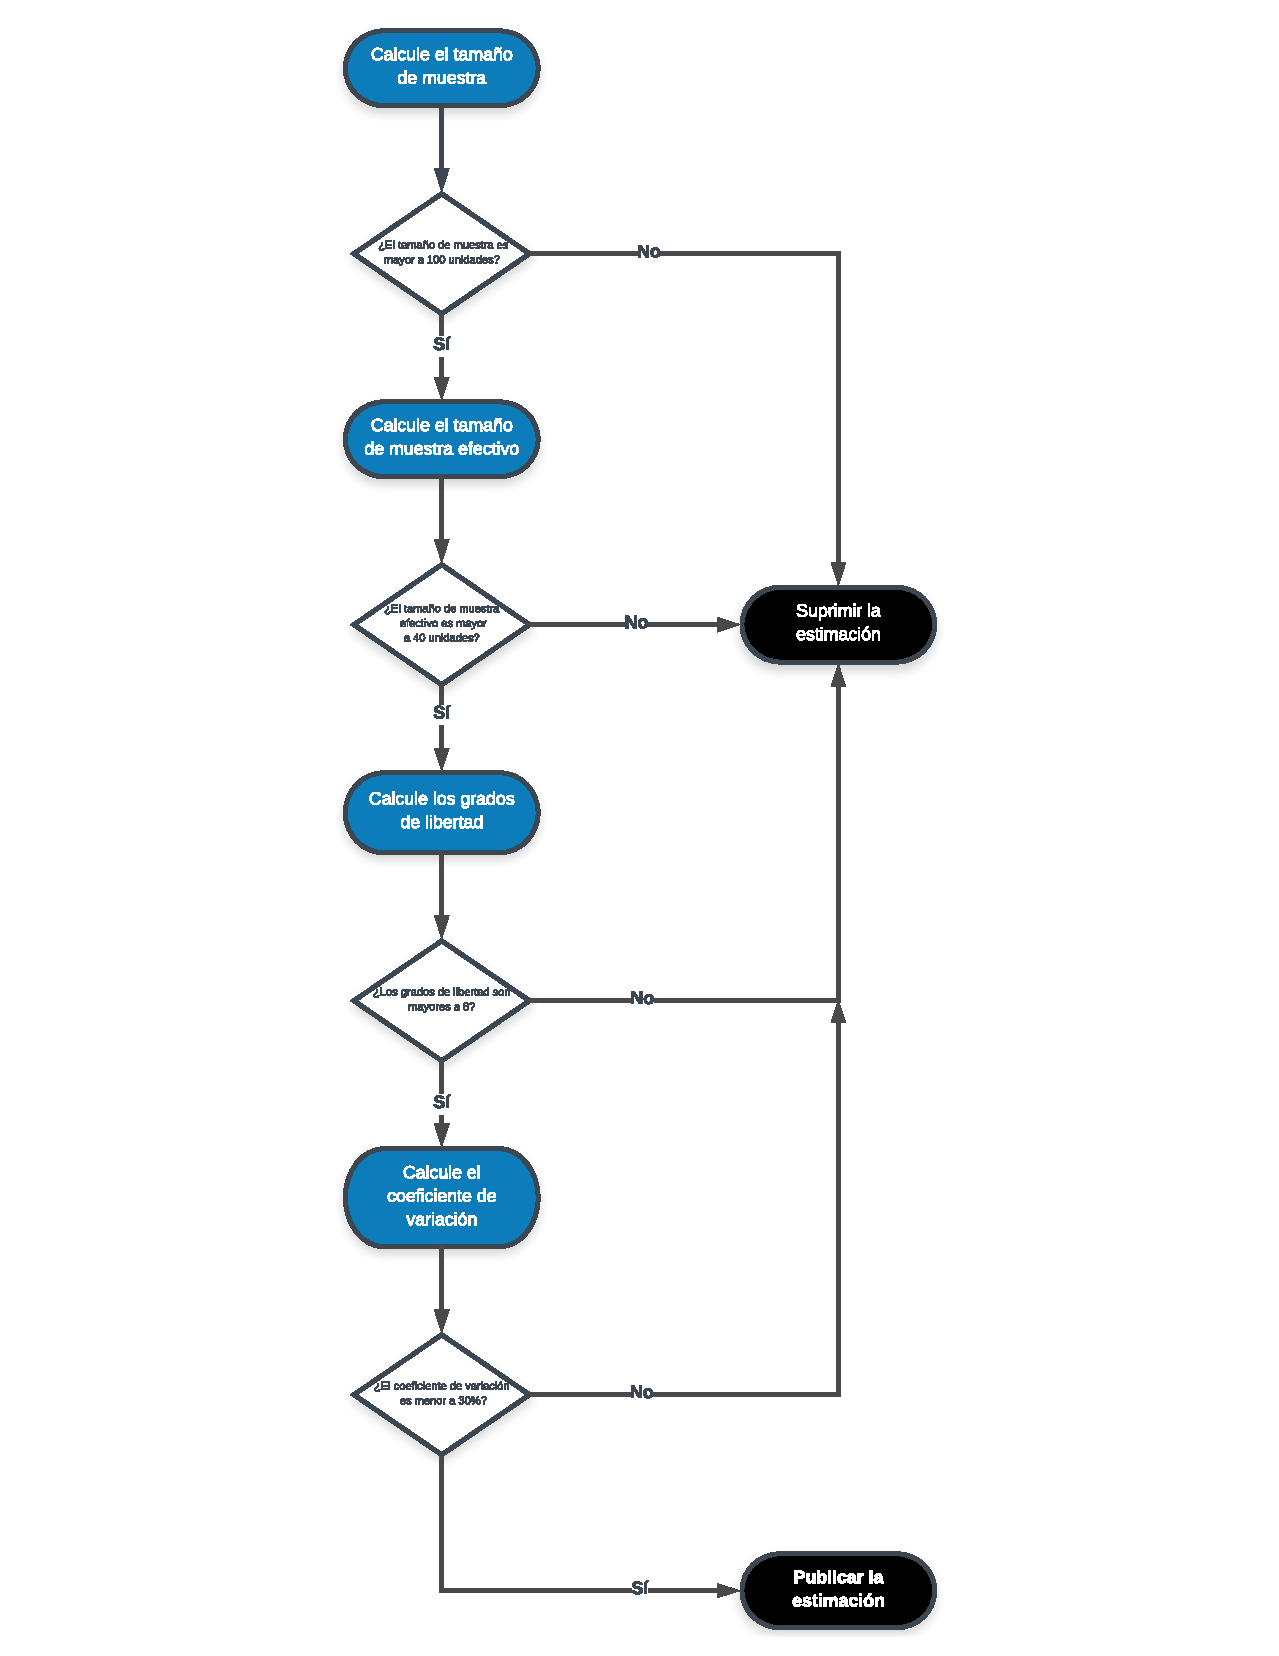
\includegraphics{Pics/14.pdf}
\caption{Ejemplo de diagramna de flujo para publicar/suprimir estimaciones en encuestas de hogares}
\end{figure}

\hypertarget{aplicacion}{%
\section{Aplicación}\label{aplicacion}}

País grande: desocupación urbana - Quintiles de ingreso - Sexo

\begin{longtable}[]{@{}lllllllllll@{}}
\toprule
Quintil Urbano & sexo & n & Deff & n.eff & gl & Desocupación\% & Li \% & Ls \% & cv \% & Alerta\tabularnewline
\midrule
\endhead
Quinto & Hombre & 29158 & 1.2 & 24293 & 4275 & 1.4 & 1.3 & 1.6 & 5.7 &\tabularnewline
Quinto & Mujer & 30848 & 1.3 & 24639 & 4215 & 1.8 & 1.7 & 2.0 & 4.9 &\tabularnewline
Cuarto & Hombre & 29245 & 1.4 & 21654 & 4584 & 2.3 & 2.1 & 2.5 & 4.8 &\tabularnewline
Cuarto & Mujer & 30094 & 1.3 & 22583 & 4574 & 2.7 & 2.4 & 2.9 & 4.3 &\tabularnewline
Tercero & Hombre & 29359 & 1.4 & 21385 & 4413 & 3.2 & 3.0 & 3.5 & 4.1 &\tabularnewline
Tercero & Mujer & 32121 & 1.5 & 21757 & 4542 & 4.0 & 3.7 & 4.3 & 3.6 &\tabularnewline
Segundo & Hombre & 30419 & 1.4 & 21806 & 4053 & 6.3 & 5.9 & 6.7 & 3.1 &\tabularnewline
Segundo & Mujer & 33619 & 1.4 & 23275 & 4169 & 7.6 & 7.2 & 8.0 & 2.6 &\tabularnewline
Primer & Hombre & 30381 & 1.5 & 20245 & 3531 & 12.7 & 12.1 & 13.3 & 2.4 &\tabularnewline
Primer & Mujer & 35233 & 1.5 & 23360 & 3700 & 12.5 & 12.0 & 13.0 & 2.1 &\tabularnewline
\bottomrule
\end{longtable}

País pequeño: desocupación urbana - Quintiles de ingreso - Sexo

\begin{longtable}[]{@{}lllllllllll@{}}
\toprule
Quintil Urbano & sexo & n & Deff & n.eff & gl & Desocupación\% & Li \% & Ls \% & cv \% & Alerta\tabularnewline
\midrule
\endhead
Quinto & Mujer & 2055 & 1.2 & 1757 & 309 & 1.0 & 0.4 & 1.6 & 30.6 & *\tabularnewline
Quinto & Hombre & 1969 & 1.1 & 1738 & 335 & 1.1 & 0.5 & 1.7 & 26.3 & *\tabularnewline
Cuarto & Hombre & 2245 & 1.2 & 1807 & 347 & 2.2 & 1.4 & 3.0 & 19.3 &\tabularnewline
Cuarto & Mujer & 2301 & 1.6 & 1466 & 357 & 4.1 & 2.7 & 5.5 & 17.5 &\tabularnewline
Tercero & Mujer & 2421 & 1.5 & 1646 & 336 & 6.1 & 4.3 & 7.9 & 15.1 &\tabularnewline
Segundo & Hombre & 2280 & 1.4 & 1654 & 295 & 5.9 & 4.3 & 7.5 & 13.8 &\tabularnewline
Tercero & Hombre & 2351 & 1.2 & 2025 & 331 & 4.6 & 3.4 & 5.8 & 13.3 &\tabularnewline
Segundo & Mujer & 2541 & 1.6 & 1547 & 310 & 10.8 & 8.0 & 13.6 & 13.1 &\tabularnewline
Primero & Mujer & 2862 & 2.0 & 1466 & 266 & 20.0 & 15.4 & 24.6 & 11.8 &\tabularnewline
Primero & Hombre & 2562 & 1.6 & 1610 & 263 & 11.9 & 9.4 & 14.5 & 10.9 &\tabularnewline
\bottomrule
\end{longtable}

País grande: desocupación rural - Quintiles de ingreso - Sexo

\begin{longtable}[]{@{}lllllllllll@{}}
\toprule
Quintil Rural & sexo & n & Deff & n.eff & gl & Desocupación\% & Li \% & Ls \% & cv \% & Alerta\tabularnewline
\midrule
\endhead
Quinto & Hombre & 5615 & 1.7 & 3279 & 282 & 0.7 & 0.4 & 1.0 & 22.1 & *\tabularnewline
Quinto & Mujer & 4637 & 1.6 & 2812 & 268 & 1.0 & 0.6 & 1.3 & 20.2 & *\tabularnewline
Cuarto & Hombre & 5506 & 1.3 & 4197 & 299 & 1.1 & 0.8 & 1.5 & 15.5 &\tabularnewline
Segundo & Hombre & 5328 & 1.3 & 4040 & 238 & 2.1 & 1.6 & 2.7 & 13.3 &\tabularnewline
Cuarto & Mujer & 4892 & 0.9 & 5176 & 291 & 1.4 & 1.1 & 1.8 & 12.5 &\tabularnewline
Tercero & Hombre & 5436 & 1.1 & 4946 & 284 & 2.1 & 1.7 & 2.6 & 11.2 &\tabularnewline
Primer & Mujer & 5100 & 1.3 & 4039 & 196 & 3.3 & 2.6 & 4.0 & 11.2 &\tabularnewline
Tercero & Mujer & 5145 & 1.3 & 4051 & 277 & 2.9 & 2.3 & 3.5 & 10.6 &\tabularnewline
Primer & Hombre & 5301 & 1.2 & 4292 & 193 & 4.2 & 3.4 & 5.0 & 9.7 &\tabularnewline
Segundo & Mujer & 5190 & 1.3 & 4101 & 238 & 3.9 & 3.2 & 4.7 & 9.6 &\tabularnewline
\bottomrule
\end{longtable}

País pequeño: desocupación rural - Quintiles de ingreso - Sexo

\begin{longtable}[]{@{}lllllllllll@{}}
\toprule
Quintil Rural & sexo & n & Deff & n.eff & gl & Desocupación\% & Li \% & Ls \% & cv \% & Alerta\tabularnewline
\midrule
\endhead
Primer & Mujer & 1788 & 0.6 & 2754 & 140 & 0.8 & 0.1 & 1.5 & 44.5 & *\tabularnewline
Cuarto & Hombre & 2112 & 1.7 & 1223 & 178 & 1.8 & 0.8 & 2.7 & 26.7 & *\tabularnewline
Segundo & Hombre & 2281 & 1.8 & 1236 & 156 & 2.6 & 1.3 & 3.9 & 25.7 & *\tabularnewline
Primer & Hombre & 1704 & 1.3 & 1324 & 137 & 2.8 & 1.4 & 4.2 & 25.5 & *\tabularnewline
Quinto & Mujer & 1780 & 1.3 & 1391 & 166 & 2.6 & 1.4 & 3.9 & 23.7 & *\tabularnewline
Segundo & Mujer & 2195 & 1.4 & 1579 & 158 & 5.3 & 2.9 & 7.6 & 22.7 & *\tabularnewline
Quinto & Hombre & 2127 & 1.4 & 1553 & 171 & 1.8 & 1.0 & 2.6 & 22.1 & *\tabularnewline
Tercero & Hombre & 2180 & 2.0 & 1068 & 169 & 3.7 & 2.1 & 5.2 & 21.4 & *\tabularnewline
Tercero & Mujer & 2023 & 1.4 & 1411 & 164 & 6.5 & 3.8 & 9.2 & 20.8 & *\tabularnewline
Cuarto & Mujer & 1942 & 1.6 & 1225 & 174 & 7.3 & 4.6 & 10.0 & 19.1 &\tabularnewline
\bottomrule
\end{longtable}

Las encuestas son instrumentos valiosos que permiten obtener información desagregada y precisa por los dominios de diseño.

A veces es posible obtener información desagregada y precisa en dominios que no fueron considerados en el diseño.

Muchas veces no es posible obtener información desagregada y precisa en dominios de interés para el seguimiento de los ODS.

Algunas Oficinas Nacionales de Estadística utilizan el coeficiente de variación como una medida única de información sobre la precisión de la cifra.

Existen otros elementos adicionales al coeficiente de variación que permiten tener una mejor panorámica de la precisión de las cifras.

Es posible extender el criterio de publicación y/o supresión de cifras a otras medidas que complementan el coeficiente de variación.

El coeficiente de variación no es simétrico con respecto a las proporciones.

Cuando las proporciones estimadas son muy pequeñas, es posible que el intervalo de confianza sea angosto y aún así tener coeficientes de variación que se salgan del umbral predefinido para publicación.

Es posible realizar una transformación sobre el coeficiente de variación que permita obtener mejores resultados en proporciones cercanas a cero.

Para las mismas desagregaciones y los mismos indicadores, las muestras de los países grandes tienen un mayor potencial de precisión en las estimaciones.

Para aumentar la precisión de los estimadores en las desagregaciones, los países podrían aumentar el tamaño de muestra de la encuesta.

Para aumentar la precisión de los estimadores en las desagregaciones, los países podrían apoyarse en información auxiliar externa a la encuesta.

Ante las limitaciones de las encuestas, los métodos de estimación en áreas pequeñas son una excelente opción para hacer frente a este reto.

\hypertarget{desafios-futuros}{%
\chapter{Desafios futuros}\label{desafios-futuros}}

La forma de medición de los indicadores sociales debe estar alineada con el diseño de la encuesta. Los equipos técnicos de los países deben ajustar sus metodologías a los requerimientos de la encuesta para proveer estadísticas oficiales que sean no sólo confiables y precisas sino eficientes en términos de los recursos que se destinan a la recolección de la información primaria, máxime cuando estos muchas veces se deben recortar por limitaciones en el presupuesto de los países.

En Latinomérica se observa un incremento progresivo de la tasa de ausencia de respuesta debido al aumento de viviendas no entrevistadas que se origina en la expansión urbana y en la desactualización de los marcos de muestreo. La continua expansión urbana en la región hace que los encuestadores afronten retos mayores cuando llegan a un área de muestreo y no encuentran la vivienda que se supone que deberían entrevistar, o en vez de una vivienda ahora encuentran un edificio de apartamentos. Con el uso, cada vez más frecuente de los dispositivos de almacenamiento electrónico y sistemas CAPI, es posible realizar un análisis mejor estructurado de los instrumentos de recolección de información. Por ejemplo, es posible programar saltos más complejos, estimar el tiempo promedio de respuesta en las preguntas del cuestionario, el tiempo promedio de respuesta en los bloques de preguntas, entre otras.

En el seguimiento a las metas de la Agenda 2030 y en la búsqueda del cumplimiento de los ODS, las Naciones Unidas ha expresado la necesidad de contar con estadísticas oficiales, no sólo a nivel nacional, sino a nivel de desagregaciones geográficas o de categorías demográficas de interés \autocite{United_Nations_2017}. Es así como se plantea la siguiente necesidad a los países:

\begin{quote}
\emph{La disponibilidad de datos desagregados, oportunos y de alta calidad es vital para la toma de decisiones basada en la evidencia y para garantizar la responsabilidad de la implementación de la Agenda 2030. El seguimiento del progreso en los Objetivos de Desarrollo Sostenible requiere una cantidad sin precedentes de datos y estadísticas en todos los niveles, lo que plantea un desafío importante para los sistemas estadísticos nacionales e internacionales. La comunidad estadística mundial está trabajando para modernizar y fortalecer los sistemas estadísticos para abordar todos los aspectos de la producción y el uso de datos para el desarrollo sostenible.}
\end{quote}

Por supuesto, la región no es ajena a este reto y debe desde ya plantearse la necesidad de crear capacidad en los equipos técnicos de los INE que deberán utilizar como insumo las encuestas de hogares y los registros administrativos para poder establecer metodologías de estimación en las desagregaciones de interés, que como mínimo deberán clasificarse por sexo, grupos etarios, ingreso, raza, etnia, estado migratorio, discapacidad y localización geográfica \autocite{United_Nations_2016}

Al respecto, uno de los primeros acercamientos al diseño de las encuestas de hogares para la publicación de estadísticas oficiales en dominios pequeños fue presentado por \textcite{Sinngh_Gambino_Mantel_1994} en donde se plantean algunas consideraciones para la estimación de indicadores sociales a nivel de dominios pequeños. Sin embargo, más allá de considerar el diseño metodológico, ahora es posible considerar otro tipo de acercamientos inferenciales que pretenden estimar indicadores a nivel de estos dominios pequeños. \textcite{Rao_Molina_2014} proveen un resumen exhaustivo de las técnicas más usadas en la diseminación de estadísticas oficiales en desagregaciones pequeñas. En América Latina, este tipo de metodologías, que utilizan como insumo las encuestas de hogares, se aplican con mayor frecuencia. Por ejemplo, \textcite{arias2007geography} realizan una estimación de la pobreza monetaria en las municipalidades de Bolivia utilizando los datos del censo poblacional del 2001; \textcite{araujo20071990} resume la experiencia ecuatoriana de la estimación de la pobreza en los municipios, cantones y provincias; \textcite{lopez2007poverty} presentan la estimación de indicadores de desarrollo humano utilizando estimación de áreas pequeñas en las municipalidades de México a través de la \emph{Encuesta Nacional de Ingresos y Gastos de los Hogares}. Finalmente, \textcite{Casas_Cordero_Valencia_Encina_Lahiri_2016} presentan un ejercicio de estimación de la pobreza en Chile utilizando la encuesta \emph{Encuesta de Caracterización Socioeconómica Nacional}.

Finalmente, vale la pena mencionar que con la llegada de los ciclos censales se actualizan los marcos de muestreo y por consiguiente la metodología de diseño y recolección de información primaria en las encuestas de hogares. En general, se debe evitar que las UPMs no tengan el mismo tamaño dentro de los estratos. Por ejemplo, en la ruralidad se pueden presentar casos en donde una única UPMs agrupa un conjunto de viviendas con demasiada heterogeneidad. Es así como es posible encontrar UPMs con pocas viviendas o UPMs con demasiadas viviendas. Esto constituye una desventaja técnica a la hora de establecer metodologías apropiadas para la recolección de la información primaria y además para la estimación de los errores de muestreo que se derivan de las encuestas de hogares. La distribución desigual de viviendas en las UPMs trae varias consecuencias negativas. Por ejemplo, las estimaciones de las varianzas son mucho más grandes y por ende las cifras oficiales serán menos precisas, necesitándose un tamaño de muestra más amplio para satisfacer un umbral de error de muestreo. Lo anterior se basa en que, en particular para la estimación de un total poblacional, el error de muestreo está en función de la siguiente expresión

\[Var(\hat{t}_y) \approx \frac{N_I^2}{n_I}\left(1-\frac{n_I}{N_I}\right)S^2_{t_{U_I}} \]

En donde \(N_I\) es número de UPMs en la población, \(n_I\) es el número de UPMs seleccionadas en la muestra de la primera etapa y \(S^2_{t_{U_I}}\) es la variación poblacional entre los totales de las UPMs. En particular \textcite[pág. 144]{SSW_2003} afirman que esta varianza se incrementa cuando la variación de los tamaños (número de viviendas) de las UPMs es alta.

\textcite{Beland_Dale_Dufour_Hamel_2005} describen los principales elementos del diseño de una encuesta de hogares y esta es una tarea que deben afrontar los equipos técnicos de los INE en términos de aprender de las experiencias del pasado para mejorar los procesos operativos, metodológicos y logísticos en las siguientes aplicaciones de las encuestas. Es así como ante la nueva oleada de censos que se avecina en la próxima década, será natural actualizar los marcos de muestreo y con ello se viene un reto para los equipos técnicos encargados de la encuestas de hogares en América Latina que consiste en evaluar el impacto del cambio de los marcos de muestreo y sus efectos en la comparabilidad de las cifras oficiales.

\hypertarget{anexos}{%
\chapter*{Anexos}\label{anexos}}
\addcontentsline{toc}{chapter}{Anexos}

\hypertarget{software}{%
\section*{Software}\label{software}}
\addcontentsline{toc}{section}{Software}

El diseño y análisis de la información proveniente de las encuestas de hogares debe contemplar el uso exhaustivo de las herramientas computacionales existentes. Esta sección revisa con detalle las aproximaciones computacionales del software estadístico utilizado para realizar cada uno de los procesos estadísticos que se necesitan para lograr el cometido de la publicación de cifras oficiales con altos niveles de precisión y confiabilidad. En particular, para los siguientes procesos:

\begin{enumerate}
\def\labelenumi{\arabic{enumi}.}
\tightlist
\item
  Selección de muestras acorde al diseño de muestreo definido
\item
  Generación de pesos de muestreo para cada individuo y hogar.
\item
  Modelación de la ausencia de respuesta e imputación estadística.
\item
  Calibración de los pesos de muestreo y ajustes por ausencia de respuesta.
\item
  Estimación de los errores de muestreo para cada indicador de interés en los cuadros de producción estadística.
\item
  Análisis de las relaciones multivariantes entre las variables de la encuesta.
\item
  Modelación de las estimaciones para la predicción del parámetro de interés en dominios pequeños.
\end{enumerate}

\textcite[sección 7.8]{United_Nations_2005} muestra la importancia de incluir la estructura del diseño de muestreo complejo en la inferencia que se realiza para la estimación de estadísticas oficiales a partir de encuestas de hogares y advierten con un ejemplo empírico que de no hacerlo, es posible que las estimaciones resultantes sean sesgadas y además sus errores de muestreo se vean subestimados. A continuación se muestran algunos de las características más importantes que los paquetes estadísticos computacionales incorporan en el manejo de datos que provienen de estructuras de muestreo complejas como las encontradas en las encuestas de hogares. Una revisión más exhaustiva y detallada que adjunta sintaxis y código computacional puede encontrarse en \textcite[Apéndice A]{Heeringa_West_Berglund_2010}.

En general, estas herramientas computacionales están pensadas para hacer más eficiente el uso de las aproximaciones de varianza en muestras complejas, así como las técnicas de replicación para obtener los estimativos de varianza inducidos por el diseño de muestreo \autocite{Westat_2007}. Algunos de estos softwares son de uso libre, aunque la mayoría corresponde a productos licenciados cuya licencia debe ser pagada. En general estos productos, además de proveer estadísticas descriptivas (como medias, totales, proporciones, percentiles y razones), permiten ajustar modelos de regresión lineales y logísticos. Todas las estadísticas resultantes están basadas en el diseño de muestreo de la encuesta.

\hypertarget{r}{%
\subsection*{R}\label{r}}
\addcontentsline{toc}{subsection}{R}

R es un software de uso libre cuyo uso es cada vez más frecuente en la investigación social, puesto que es muy probable encontrar los más recientes hallazgos científicos programados en este software \autocite{R_2017}. Al ser de uso libre, los investigadores pueden subir sus propias colecciones de funciones computacionales al repositorio oficial (\texttt{CRAN}) y ponerlas a disposición de la comunidad. El paquete \texttt{samplesize4surveys} \autocite{ss4s} permite determinar el tamaño de muestra de individuos y hogares en encuestas de hogares repetidas, tipo panel y con rotación. Los paquetes \texttt{sampling} \autocite{Yves} y \texttt{TeachingSampling} \autocite{TS} permiten seleccionar muestras probabilísticas desde los marcos de muestreo bajo un gran variedad de diseños y algoritmos de muestreo. El paquete \texttt{survey} \autocite{TL}, una vez que el diseño de muestreo ha sido predefinido mediante la función \texttt{svydesign()}, permite analizar datos provenientes de encuestas de hogares y obtener estimaciones apropiadas de los errores estándar.

\hypertarget{spss}{%
\subsection*{SPSS}\label{spss}}
\addcontentsline{toc}{subsection}{SPSS}

El módulo \texttt{complex\ samples} de \texttt{SPSS} \autocite{IBM_2017} incorpora la selección de muestras complejas mediante la definición de un esquema de muestreo establecido por el usuario. Luego, es necesario crear un plan de análisis mediante la asignación de variables de diseño, métodos de estimación y tamaños de las unidades de muestreo. Una vez definido el plan de muestreo, el módulo integra la posibilidad de estimar conteos, estadísticas descriptivas y celdas de tablas cruzadas. También es posible realizar estimaciones de razones y de coeficientes de regresión en modelos lineales, junto con las respectivas estadísticas de pruebas de hipótesis. Por último el módulo permite estimar modelos no lineales, como regresiones logísticas, regresiones ordinales o regresiones de Cox.

\hypertarget{sas}{%
\subsection*{SAS}\label{sas}}
\addcontentsline{toc}{subsection}{SAS}

Este software estadístico incluye un procedimiento para la selección de muestras probabilísticas llamado \texttt{SURVEYSELECT} que integra los métodos de selección más comunes como muestreo aleatorio simple, muestreo sistemático, muestreo con probabilidad proporcional al tamaño, y algunas herramientas de afijación en los estratos. Para analizar los datos provenientes de muestras complejas se han programado algunos procedimientos \autocite{SAS_2017}. \texttt{SURVEYMEANS}, que estima totales, medias, proporciones, y percentiles, junto con sus respectivos errores estándar, límites de los intervalos de confianza y pruebas de hipótesis. \texttt{SURVEYFREQ}, estima las estadísticas descriptivas (como totales y proporciones) de interés en tablas de una y dos vías, brinda las estimaciones del error de muestreo, y realiza un análisis de la bondad del ajuste de las estimaciones, independencia, riesgos y razones de \emph{odds}. \texttt{SURVEYREG} y \texttt{SURVEYLOGISTIC} ajustan modelos de regresión lineal y logísticas, respectivamente. Estos procedimientos estiman los coeficientes de regresión, con sus respectivos errores, y adjunta un análisis exhaustivo de las propiedades de los modelos. Por último, \texttt{SURVEYPHREG} ajusta modelos de riesgos utilizando técnicas de máxima-pseudo verosimilitud.

\hypertarget{stata}{%
\subsection*{STATA}\label{stata}}
\addcontentsline{toc}{subsection}{STATA}

El entorno \texttt{svy} provee un conjunto de herramientas para hacer una inferencia apropiada de las estadísticas oficiales provenientes de encuestas de hogares \autocite{STATA_2017}. El comando \texttt{svyset} permite especificar las variables que identifican las características del diseño de muestreo de la encuesta, como los pesos de muestreo, los conglomerados y los estratos. El comando \texttt{svydescribe} proporciona tablas que describen los estratos y las unidades de muestra para una determinada etapa de la encuesta. Una vez cargadas las definiciones del diseño de muestreo, cualquier modelo puede ser estimado y sus estadísticos resultantes estarán basados en el diseño de muestreo de la encuesta. El entorno \texttt{svy} también permite la ejecución de algunos comandos predictivos.

\hypertarget{algunas-encuestas-de-hogares-en-la-region}{%
\section*{Algunas encuestas de hogares en la región}\label{algunas-encuestas-de-hogares-en-la-region}}
\addcontentsline{toc}{section}{Algunas encuestas de hogares en la región}

Esta sección presenta una breve descripción del estado de la situación de las encuestas de hogares en la región. Aunque no se pretende hacer un resumen exhaustivo de cada encuesta y de sus componentes metodológicos, con seguridad el lector podrá enterarse de las características principales de la encuestas de hogares y sus condiciones de aplicación.

\hypertarget{argentina}{%
\subsection*{Argentina}\label{argentina}}
\addcontentsline{toc}{subsection}{Argentina}

El Instituto Nacional de Estadística y Censo lleva a cabo de forma trimestral la \emph{Encuesta Permanente de Hogares} la cual permite caracterizar la situación social de los individuos y las familias teniendo en cuenta su inserción en la estructura social y económica \autocite{INDEC-AR}. Esta encuesta revela información sobre características demográficas básicas de los miembros del hogar y su situación laboral, ingresos de los individuos, así como sus características educacionales y de migración. También permite caracterizar las viviendas.

Por otro lado, la \emph{Encuesta Nacional de Gastos de los Hogares} proporciona información sobre los hogares argentinos mediante el relevamiento de sus gastos e ingresos. Sus resultados contribuyen con la elaboración de la canasta de bienes y servicios que se utiliza para medir el índice de precios al consumidor, así como aportan información para la estimación de la pobreza y la producción de indicadores de la economía nacional \autocite{INDEC-AR2}.

\hypertarget{bolivia}{%
\subsection*{Bolivia}\label{bolivia}}
\addcontentsline{toc}{subsection}{Bolivia}

El objetivo principal de la \emph{Encuesta Continua de Hogares} aplicada anualmente por el Instituto Nacional de Estadística es suministrar información sobre las condiciones de vida de los hogares, a partir de la recopilación de información de variables económicas y demográficas de la población para le diseño de programas sociales y formulación, evaluación y seguimiento de las políticas públicas. Dentro de los ejes temáticos que aborda la encuesta se encuentran la estimación de las necesidades básicas insatisfechas, el acceso a los servicios públicos, la caracterización demográfica de los individuos, los desplazamientos de la población en los últimos cinco años, el estado de salud de los miembros del hogar, las características educativas, las condiciones de ocupación, los ingresos percibidos y los gastos del hogar. Esta encuesta permite medir oportunamente los indicadores de pobreza de la población boliviana, así como el acceso a la vivienda, los servicios básicos, la educación, entre otros. Mediante la EH, el INE obtiene estadísticas e indicadores socioeconómicos y demográficos de la población que son necesarias para la formulación, evaluación, monitoreo y seguimiento de las políticas del estado \autocite{INE-BO}.

\hypertarget{brasil}{%
\subsection*{Brasil}\label{brasil}}
\addcontentsline{toc}{subsection}{Brasil}

La \emph{Pesquisa Nacional por Amostra de Domicílios} es implementada anualmente por el Instituto Brasileiro de Geografia e Estatística. Esta encuesta tiene como objetivo producir información básica para el estudio de la evolución económica de Brasil y la publicación continua de indicadores demográficos. Los constructos de ingreso, gastos y empleo son evaluados de forma continua, mientras que anualmente se abordan otros módulos de interés. Otros temas adicionales investigados en la encuesta están relacionados con las características de la vivienda, migración de los individuos del hogar, trabajo infantil, fecundidad, salud y seguridad alimentaria, uso de las tecnologías de información, transferencias de renta, uso del tiempo, entre otros \autocite{IBGE-BR_2017}.

La \emph{Pesquisa de Orçamentos Familiares} tiene como propósito obtener informaciones generales sobre domicilios, familias y personas, hábitos de consumo, gastos y recibos de las familias encuestadas, teniendo como unidad de recolección los domicilios. Permite actualizar la canasta básica de consumo y obtiene nuevas estructuras de ponderación para los índices de precios que componen el Sistema Nacional de Índices de Precios al Consumidor del IBGE y otras instituciones \autocite{IBGE-BR2018}

\hypertarget{chile}{%
\subsection*{Chile}\label{chile}}
\addcontentsline{toc}{subsection}{Chile}

El Ministerio de Desarrollo Social aplica la \emph{Encuesta de Caracterización Socioeconómica Nacional} de forma bianual y su objetivo es conocer periódicamente la situación de los hogares y de la población, especialmente de aquella en situación de pobreza, con relación a aspectos demográficos, de educación, salud, vivienda, trabajo e ingresos. De esta forma, la encuesta permite estimar la magnitud de la pobreza y la distribución del ingreso; identificar carencias y demandas de la población en las áreas señaladas; y evaluar las distintas brechas que separan a los diferentes segmentos sociales y ámbitos territoriales. Esta encuesta también permite medir la eficacia de los programas sociales que ha implementado el gobierno para la toma de decisiones de política pública. Entre otros, la encuesta se compone de los módulos de registro, que incluye información de identificación de los hogares; educación, que indaga por la situación educacional de los miembros del hogar y la cobertura del sistema educativo; trabajo, que permite conocer la evolución de la situación laboral y ocupacional para formular y evaluar políticas públicas; ingresos, que permite investigar las condiciones de vida de los miembros del hogar; salud, en donde se indaga por la cobertura de los programas públicos \autocite{MDS-CL_2015}.

La \emph{Encuesta de Presupuestos Familiares} es una encuesta socioeconómica aplicada a hogares, cuyo propósito es recopilar información sobre gastos en los que estos incurren y los ingresos que perciben en un período de tiempo determinado. La información que recoge la EPF es la base para elaborar la canasta de bienes y servicios con la cual se calcula el Índice de Precios al Consumidor y también se utiliza para actualizar las líneas de pobreza extrema y pobreza empleadas en las estadísticas oficiales de Chile \autocite{INE_CL}.

\hypertarget{colombia}{%
\subsection*{Colombia}\label{colombia}}
\addcontentsline{toc}{subsection}{Colombia}

El Departamento Nacional de Estadística aplica la \emph{Gran Encuesta Integrada de Hogares} de forma mensual. Esta encuesta tiene como objetivo general proporcionar información económica básica con énfasis en las características de la fuerza de trabajo. Además indaga por constructos sociales y económicos. Dentro de la temática social, se pregunta por el acceso a la educación formal, condiciones de calidad de vida, ingresos y gastos, trabajo infantil y aspectos de seguridad y convivencia ciudadana. La temática económica indaga aspectos relacionados con industria, comercio, servicios y transporte. El instrumento de recolección de la encuesta está dividido en capítulos que abordan la información relacionada con la vivienda y el hogar, además de hacer un registro de las personas que conforman el hogar y su relación con el jefe de hogar, estableciendo así una caracterización general de la población. Por lo demás también indaga por el acceso a la seguridad social en salud, las características educativas de las población mayor de tres años y clasifica a las personas mayores de 10 años en las categorías establecidas para la fuerza de trabajo \autocite{DANE-COL_2017}.

La \emph{Encuesta Nacional de Presupuestos de los Hogares} es una investigación dirigida a los hogares, en la cual se indagan en forma detallada todos los ingresos de los miembros del hogar de 10 años y más (ingresos por trabajo, ingresos de capital, subsidios, transferencias, ingresos ocasionales, etc) así como todos los posibles gastos en que puede incurrir un hogar, captados con diferentes periodicidades (semanal, mensual, trimestral y anual). Dentro de sus objetivos específicos está el obtener información para realizar actualizaciones del IPC, estimar líneas de indigencia y pobreza, caracterizar la distribución del ingreso del hogar con características demográficas, educativas y económicas, etc. \autocite{DANE-COL_2018}

\hypertarget{costa-rica}{%
\subsection*{Costa Rica}\label{costa-rica}}
\addcontentsline{toc}{subsection}{Costa Rica}

La \emph{Encuesta Nacional de Hogares}, llevada a cabo por el Instituto Nacional de Estadística y Censos de forma anual, tiene como objetivo producir estimaciones del nivel de bienestar de la población, especialmente centrados en la conformación del ingreso de los hogares, su distribución y características de los hogares y la población en situación de pobreza. El constructo principal y la motivación de esta encuesta está referido a la pobreza multidimensional y la desigualdad midiendo el ingreso promedio de los hogares por fuente y su distribución, su incidencia y severidad, así como las brechas y perfiles. Esta encuesta permite obtener estas estimaciones a nivel de región y ha incluido algunos módulos especiales de victimización, gasto en los hogares y acceso a la salud \autocite{INEC-CR_2017}.

La \emph{Encuesta Nacional de Ingresos y Gastos} de los Hogares proporciona datos económicos de los hogares para conocer las diversas fuentes de ingresos que tienen éstos y cómo distribuyen sus ingresos en la adquisición de los diferentes bienes y servicios. La encuesta suministra gran parte de la información necesaria para estimar la secuencia de cuentas del Sector Hogares, dentro del sistema de Cuentas Nacionales del país. También brinda los datos necesarios para actualizar la canasta de bienes y servicios que componen el Índice de Precios al Consumidor (IPC); entre otros estudios sobre la estructura de gastos de los hogares y la distribución del ingreso \autocite{INEC-CR_2018}.

\hypertarget{cuba}{%
\subsection*{Cuba}\label{cuba}}
\addcontentsline{toc}{subsection}{Cuba}

La Oficina Nacional de Estadística e Información aplica anualmente la \emph{Encuesta Nacional de Ocupación} y la \emph{Encuesta de Situación Económica de los Hogares}. Lo objetivos de estas investigaciones se centran en la caracterización de la población en edad de trabajar y su ocupación, así como en obtener indicadores para la toma de decisiones en materia de políticas sociales y económicas \autocite{ONE-CU}.

Estas encuestas investigan temas relacionados como las características de las viviendas, la educación en los hogares, las características económicas de los miembros del hogar (para las personas mayores de 15 años), la movilidad laboral y los ingresos en el hogar.

\hypertarget{ecuador}{%
\subsection*{Ecuador}\label{ecuador}}
\addcontentsline{toc}{subsection}{Ecuador}

El Instituto Nacional de Estadística y Censos cuenta con el Sistema Integrado de Encuestas a Hogares con el cual se produce información de las características demográficas y económicas de los hogares y personas. Entre otras, el sistema cuenta con la \emph{Encuesta de Empleo, Desempleo y Subempleo en Área Urbana y Rural}, con periodicidad mensual; la \emph{Encuesta Nacional de Ingresos y Gastos de los Hogares Urbanos y Rurales}, con periodicidad quinquenal; y la \emph{Encuesta de Condiciones de Vida}, con periodicidad cuatrienal. Las anteriores encuestas cuentan con temas en común, como condiciones de vivienda, caracterización de los hogares, educación de los miembros del hogar, condición de la actividad económica de los individuos, acceso a servicios públicos e ingreso \autocite{INEC-EC}.

Por ejemplo, la \emph{Encuesta de Condiciones de Vida} permite obtener indicadores sobre los niveles de vida y el bienestar de la población relacionando varios factores como educación, salud, pobreza e inequidad para la aplicación de política pública. La ECV 2013 -- 2014 incluye temas nuevos como hábitos, prácticas y uso del tiempo de los hogares, bienestar psicosocial, percepción del nivel de vida, capital social, seguridad ciudadana y retorno migratorio \autocite{INEC2-EC}.

\hypertarget{el-salvador}{%
\subsection*{El Salvador}\label{el-salvador}}
\addcontentsline{toc}{subsection}{El Salvador}

La \emph{Encuesta de Hogares de Propósitos Múltiples} es implementada anualmente por la Dirección General de Estadística y Censos y su objetivo es generar información estadística relacionada con las condiciones económicas y demográficas de la población con el fin de evaluar y focalizar las políticas públicas del gobierno para elevar el bienestar de la población. Esta encuesta indaga por la información general de los miembros del hogar, su situación educacional (analfabetismo, escolaridad y asistencia), también pregunta por las características de la vivienda y la situación de ocupación de la población Contiene a su vez un módulo de actividad del productor agropecuario que recolecta información acerca de la tenencia de la tierra, superficie cultivada, y la actividad agropecuaria del entrevistado. Por último también pregunta acerca de variables de salud, dinámica de las remesas y los gastos del hogar \autocite{DIGESTYC-SV}.

La \emph{Encuesta de Ingresos y Gastos de los Hogares} permite determinar la canasta de mercado para el desarrollo del Índice de Precios al Consumidor (IPC), el consumo privado en las Cuentas Nacionales (CN) y para análisis de bienestar y pobreza. La encuesta también mide la educación, el empleo, las condiciones de la vivienda, la posesión de bienes durables, la construcción y los otros negocios y actividades agrícolas relacionados al hogar \autocite{DIGESTYC2-SV}.

\hypertarget{guatemala}{%
\subsection*{Guatemala}\label{guatemala}}
\addcontentsline{toc}{subsection}{Guatemala}

El Instituto Nacional de Estadística aplica de manera semestral la \emph{Encuesta Nacional de Empleo e Ingresos}. Los objetivos de esta encuesta son dar seguimiento a un conjunto básico de variables e indicadores del mercado laboral y producir información que permita conocer el comportamiento y evolución del empleo, el desempleo, las características, composición, estructura y funcionamiento del mercado de trabajo. Además de investigar aspectos generales del mercado laboral, esta encuesta indaga las características de informalidad, ocupación y formas de contratación. Tiene un componente de ingresos, así como algunos aspectos demográficos y de educación en los hogares de Guatemala. Algunos cambios recientes han incluido módulos de uso del tiempo y uso de las tecnologías de información \autocite{INE-GT}.

La \emph{Encuesta Nacional de Condiciones de Vida} tiene como principal objetivo, conocer y evaluar las condiciones de vida de la población, así como determinar los niveles de pobreza existentes en Guatemala y los factores que los determinan caracterizando a la población pobre t no pobre del país, brindando resultados a nivel nacional, regional y departamental \autocite{INE2-GT}.

\hypertarget{honduras}{%
\subsection*{Honduras}\label{honduras}}
\addcontentsline{toc}{subsection}{Honduras}

La \emph{Encuesta Permanente de Hogares de Propósitos Múltiples} es una investigación semestral dirigida por el Instituto Nacional de Estadística de Honduras con el fin de recolectar información sobre las características generales de la población hondureña, en términos de vivienda, tasas de ocupación, desocupación y subempleo, ingreso en los hogares y acceso a las tecnologías de la información \autocite{INE-HN}.

La \emph{Encuesta de Condiciones de Vida de los Hogares} es una investigacion de carácter multipropósito que permite conocer los diferentes aspectos y dimensiones del bienestar de los hogares. Incluye, además de los ingresos y gastos de las unidades familiares, un conjunto de variables que describen los niveles de vida de los hogares. En este sentido esta publicación incorpora información sobre: Características de la vivienda, demografía, migración, educación, salud, antropometría, mercado laboral (género, personas con problemas laborales, trabajo infantil y juvenil), ingresos y gasto de los hogares, pobreza y otros temas de importancia \autocite{INE2-HN}.

\hypertarget{mexico}{%
\subsection*{México}\label{mexico}}
\addcontentsline{toc}{subsection}{México}

La \emph{Encuesta Nacional de Ocupación y Empleo} aplicada cada dos años por el Instituto Nacional de Estadística y Geografía tiene como objetivo proporcionar un panorama estadístico del comportamiento de los ingresos y gastos de los hogares en cuanto a su monto, procedencia y distribución; adicionalmente, ofrece información sobre las características ocupacionales y demográficas de los integrantes del hogar, así como las características de la infraestructura de la vivienda y el equipamiento del hogar. Además de lo anterior, la encuesta cubre algunos constructos como percepciones y erogaciones financieras y de capital de los hogares y sus integrantes, características de la vivienda, características demográficas de los residentes de la vivienda, condición de actividad y características ocupacionales de los integrantes del hogar de 12 y más años, equipamiento del hogar y acceso a servicios \autocite{INEGI-MX}.

La \emph{Encuesta Nacional de Ingresos y Gastos de los Hogares} tiene como objetivo proporcionar un panorama estadístico del comportamiento de los ingresos y gastos de los hogares en cuanto a su monto, procedencia y distribución; adicionalmente, ofrece información sobre las características ocupacionales y sociodemográficas de los integrantes del hogar, así como las características de la infraestructura de la vivienda y el equipamiento del hogar \autocite{INEGI2-MX}.

\hypertarget{nicaragua}{%
\subsection*{Nicaragua}\label{nicaragua}}
\addcontentsline{toc}{subsection}{Nicaragua}

Nicaragua lleva a cabo de forma trimestral la \emph{Encuesta Nacional de Hogares Sobre la Medición de Niveles de Vida}, a través del Instituto Nacional de Información de Desarrollo, cuyo objetivo general es producir información continua sobre características ocupacionales, demográficas y evolución de la pobreza. Esta encuesta indaga exhaustivamente acerca de las características demográficas de todos los miembros del hogar, además de la actividad económica y condición de los individuos en edad de trabajar y sus ingresos. Indaga también por el estado de la vivienda y sus características. Esta encuesta también dispone de las variables necesarias para la construcción de otras medidas de bienestar, como agregado de ingreso, necesidades básicas insatisfechas, etc. \autocite{INIDE-NI}.

\hypertarget{panama}{%
\subsection*{Panamá}\label{panama}}
\addcontentsline{toc}{subsection}{Panamá}

El Instituto Nacional de Estadística y Censo de Panamá aplica anualmente la \emph{Encuesta de Propósitos Múltiples} cuyos objetivos están encaminados a la producción de estadísticas de empleo e ingresos y a la estimación de la situación del mercado Laboral. Como la principal finalidad de la encuesta es la medición de los cambios del mercado laboral, se indaga por la condición de actividad económica, ocupación, lugar de trabajo e ingresos. También se debe resaltar que la encuesta aborda, de manera no continua, algunos temas relacionados con el acceso a la tecnología, el interés y colaboración con actividades de protección y conservación de los recursos naturales, dinámica de turismo en los hogares, identificación de recibo o envío de remesas y migración (desplazamiento interno y externo de la población durante un intervalo), así como el uso de servicios financieros \autocite{INEC-PA}.

La \emph{Encuesta de Ingresos y Gastos de los Hogares} se realiza para actualizar la información de los ingresos de los hogares en panamá y como estos distribuyen los presupuestos para obtener diferentes bienes y servicios. La información recopilada tiene como principales objetivos obtener coeficientes de ponderación y canastas de consumo que serán utilizadas para el cálculo del IPC y la CBFA. Por otra parte permite estructurar la demanda de los hogares en bienes de consumo privado \autocite{INEC2-PA}.

\hypertarget{paraguay}{%
\subsection*{Paraguay}\label{paraguay}}
\addcontentsline{toc}{subsection}{Paraguay}

La \emph{Encuesta Permanente de Hogares} ejecutada anualmente por la Dirección General de Estadística, Encuestas y Censos tiene como objetivo la generación de indicadores anuales sobre las principales características de las condiciones de vida de la población y sus resultados son utilizados para las estimaciones de pobreza. Algunos de los constructos que investiga esta encuesta se relacionan con las características de las viviendas, educación de los miembros del hogar, salud, empleo e ingresos, condición de ocupación, acceso a programas sociales del gobierno y remesas \autocite{DGEEC-PY}.

La \emph{Encuesta de Ingresos y Gastos y de Condiciones de Vida} tiene como principal objetivo actualizar la estructura de la Canasta Básica de Alimentos y la Canasta Total Familiar, cuyos valores constituyen las líneas de pobreza, así como el de caracterizar y analizar las Condiciones de Vida de la Población del Paraguay. Esta información es recopilada a través de cuestionarios que recogen datos acerca de temas de educación, salud, ingresos, actividades independientes no agropecuarias, perfiles de ingresos y de tipo productivo, etc. \autocite{DGEEC2-PY}.

\hypertarget{peru}{%
\subsection*{Perú}\label{peru}}
\addcontentsline{toc}{subsection}{Perú}

La \emph{Encuesta Nacional de Hogares sobre Condiciones de Vida y Pobreza} es una investigación mensual que realiza el Instituto Nacional de Estadística e Informática cuyo objetivo es la obtención de información estadística, social, demográfica y económica, proveniente de los hogares para el cálculo de indicadores para la medición de aspectos económicos y sociales; y conocer y explicar los determinantes o factores causales del comportamiento de dichos aspectos para el diseño, monitoreo y medición de resultados de las políticas públicas. Dentro de los módulos que la encuesta aborda se encuentran la caracterización de la vivienda y el hogar, la educación de los miembros del hogar, así como su estado de salud, la condición de actividad de empleo, ingresos y gastos, acceso a programas sociales, participación ciudadana, así como la percepción de la gobernabilidad y algunos tópicos concernientes al fenómeno de la discriminación \autocite{INEI-PE_2016}.

\hypertarget{republica-dominicana}{%
\subsection*{República Dominicana}\label{republica-dominicana}}
\addcontentsline{toc}{subsection}{República Dominicana}

La Oficina Nacional de Estadística cuenta con un Sistema Integrado de Encuestas de Hogares que agrupa, entre otras, a la \emph{Encuesta Nacional de Hogares de Propósitos Múltiples}, con periodicidad anual y la \emph{Encuesta Nacional de Fuerza de Trabajo}, con periodicidad semestral. La primera es una encuesta orientada a recopilar periódicamente datos sobre diferentes temas sociales, económicos y ambientales; mientras que la segunda está orientada a obtener indicadores de la población en edad de trabajar y su ocupación. Algunos de los aspectos principales que evalúa el sistema de encuestas de hogares están relacionados con las condiciones y características de las viviendas y personas, así como con la educación de los miembros del hogar, el acceso a tecnologías de información y algunas características de seguridad ciudadana y convivencia \autocite{ONE-DO}.

Por ejemplo, la Encuesta Nacional de Ingresos y Gastos de los Hogares es un estudio estadístico que se realiza generalmente cada 10 años para conocer la distribución del gasto en bienes y servicios de consumo de los hogares, así como los ingresos que éstos obtienen por diferentes fuentes para financiar su consumo. Dentro de sus objetivos se encuentra el obtener información para conocer el nivel y la estructura de los gastos de consumo de los hogares y su distribución en rubros de: alimentos y bebidas no alcohólicas; bebidas alcohólicas, tabaco y estupefacientes; prendas de vestir y calzado; alojamiento, agua, electricidad, gas, y otros combustibles; muebles, artículos para el hogar y para la conservación ordinaria del hogar; salud; transporte; comunicaciones; recreación y cultura; educación; restaurantes y hoteles y, bienes y servicios diversos \autocite{ONE2-DO}.

\hypertarget{uruguay}{%
\subsection*{Uruguay}\label{uruguay}}
\addcontentsline{toc}{subsection}{Uruguay}

El Instituto Nacional de Estadística aplica mensualmente la \emph{Encuesta Continua de Hogares} que brinda los indicadores oficiales del mercado laboral (actividad, empleo y desempleo) y de ingresos de los hogares y las personas. Además esta encuesta permite estimar la proporción de hogares y personas por debajo de la línea de pobreza y de indigencia de forma anual. El cuestionario de la encuesta indaga por las características de las viviendas y de los hogares, así como las características demográficas de los miembros del hogar y algunas variables de migración, acceso a la salud, educación, alimentación y uso de las tecnologías de información. De la misma forma, la encuesta aborda de manera exhaustiva los constructos de actividad laboral, ingresos y egresos personales y del hogar \autocite{INE-UY_2016}.

La \emph{Encuesta de Gastos e Ingresos de los Hogares}, se realiza aproximadamente cada 10 años y permite conocer la realidad económica y social del país. A partir de los resultados obtenidos, se podrá elaborar una canasta actualizada para el Índice de Precios al Consumo (IPC) y también determinar las líneas de indigencia y de pobreza nacionales. Esta es una encuesta muy importante, ya que a partir de los datos brindados, se puede obtener la información de base para elaborar indicadores que interesan a toda la sociedad, como son los de inflación y pobreza \autocite{INE2-UY}.

\hypertarget{venezuela}{%
\subsection*{Venezuela}\label{venezuela}}
\addcontentsline{toc}{subsection}{Venezuela}

La \emph{Encuesta de Hogares por Muestreo} es una investigación que desarrolla el Instituto Nacional de Estadística con periodicidad semestral. Esta encuesta de propósitos múltiples brinda información sobre la estructura y evolución del mercado de trabajo, así como de las características económicas y demográficas de la población. Algunos de las temáticas más relevantes de esta encuesta se centran en la actividad económica de los miembros del hogar y su estado de empleo, así como la caracterización de las viviendas y de los hogares y algunas variables educativas, que dan origen a indicadores de analfabetismo. Asimismo, la \emph{Encuesta Nacional de Presupuestos Familiares}, es una investigación por muestreo dirigida a los hogares, que tiene por objeto obtener información sobre sus ingresos, egresos, características de las viviendas que habitan, composición de los hogares y otras variables económicas y sociales de sus miembros. Dentro de sus objetivos se encuentra conocer los cambios ocurridos en los patrones de consumo de los hogares, actualizar la canasta de bienes y servicios y las ponderaciones del IPC, etc. \autocite{INE-VE}.

\newpage
\blandscape

\begin{longtable}[]{@{}llllll@{}}
\caption{\emph{Características de las algunas encuestas repetidas en América Latina.}}\tabularnewline
\toprule
\begin{minipage}[b]{0.13\columnwidth}\raggedright
País\strut
\end{minipage} & \begin{minipage}[b]{0.38\columnwidth}\raggedright
Nombre de la encuesta\strut
\end{minipage} & \begin{minipage}[b]{0.06\columnwidth}\raggedright
Tipo\strut
\end{minipage} & \begin{minipage}[b]{0.08\columnwidth}\raggedright
Periodicidad\strut
\end{minipage} & \begin{minipage}[b]{0.06\columnwidth}\raggedright
Rotación\strut
\end{minipage} & \begin{minipage}[b]{0.13\columnwidth}\raggedright
Muestra de viviendas\strut
\end{minipage}\tabularnewline
\midrule
\endfirsthead
\toprule
\begin{minipage}[b]{0.13\columnwidth}\raggedright
País\strut
\end{minipage} & \begin{minipage}[b]{0.38\columnwidth}\raggedright
Nombre de la encuesta\strut
\end{minipage} & \begin{minipage}[b]{0.06\columnwidth}\raggedright
Tipo\strut
\end{minipage} & \begin{minipage}[b]{0.08\columnwidth}\raggedright
Periodicidad\strut
\end{minipage} & \begin{minipage}[b]{0.06\columnwidth}\raggedright
Rotación\strut
\end{minipage} & \begin{minipage}[b]{0.13\columnwidth}\raggedright
Muestra de viviendas\strut
\end{minipage}\tabularnewline
\midrule
\endhead
\begin{minipage}[t]{0.13\columnwidth}\raggedright
Argentina\strut
\end{minipage} & \begin{minipage}[t]{0.38\columnwidth}\raggedright
Encuesta Permanente de Hogares\strut
\end{minipage} & \begin{minipage}[t]{0.06\columnwidth}\raggedright
Panel\strut
\end{minipage} & \begin{minipage}[t]{0.08\columnwidth}\raggedright
Trimestral\strut
\end{minipage} & \begin{minipage}[t]{0.06\columnwidth}\raggedright
50\%\strut
\end{minipage} & \begin{minipage}[t]{0.13\columnwidth}\raggedright
25000\strut
\end{minipage}\tabularnewline
\begin{minipage}[t]{0.13\columnwidth}\raggedright
Bolivia\strut
\end{minipage} & \begin{minipage}[t]{0.38\columnwidth}\raggedright
Encuesta Continua de Hogares\strut
\end{minipage} & \begin{minipage}[t]{0.06\columnwidth}\raggedright
Panel\strut
\end{minipage} & \begin{minipage}[t]{0.08\columnwidth}\raggedright
Anual\strut
\end{minipage} & \begin{minipage}[t]{0.06\columnwidth}\raggedright
25\%\strut
\end{minipage} & \begin{minipage}[t]{0.13\columnwidth}\raggedright
10000\strut
\end{minipage}\tabularnewline
\begin{minipage}[t]{0.13\columnwidth}\raggedright
Brasil\strut
\end{minipage} & \begin{minipage}[t]{0.38\columnwidth}\raggedright
Pesquisa Nacional por Amostra de Domicilios\strut
\end{minipage} & \begin{minipage}[t]{0.06\columnwidth}\raggedright
Repetida\strut
\end{minipage} & \begin{minipage}[t]{0.08\columnwidth}\raggedright
Anual\strut
\end{minipage} & \begin{minipage}[t]{0.06\columnwidth}\raggedright
-\strut
\end{minipage} & \begin{minipage}[t]{0.13\columnwidth}\raggedright
115000\strut
\end{minipage}\tabularnewline
\begin{minipage}[t]{0.13\columnwidth}\raggedright
Brasil\strut
\end{minipage} & \begin{minipage}[t]{0.38\columnwidth}\raggedright
Pesquisa Nacional por Amostra de Domicilios Continua\strut
\end{minipage} & \begin{minipage}[t]{0.06\columnwidth}\raggedright
Panel\strut
\end{minipage} & \begin{minipage}[t]{0.08\columnwidth}\raggedright
Mensual\strut
\end{minipage} & \begin{minipage}[t]{0.06\columnwidth}\raggedright
20\%\strut
\end{minipage} & \begin{minipage}[t]{0.13\columnwidth}\raggedright
70000\strut
\end{minipage}\tabularnewline
\begin{minipage}[t]{0.13\columnwidth}\raggedright
Chile\strut
\end{minipage} & \begin{minipage}[t]{0.38\columnwidth}\raggedright
Encuesta de Caracterización Socioeconómica Nacional\strut
\end{minipage} & \begin{minipage}[t]{0.06\columnwidth}\raggedright
Repetida\strut
\end{minipage} & \begin{minipage}[t]{0.08\columnwidth}\raggedright
Bienal\strut
\end{minipage} & \begin{minipage}[t]{0.06\columnwidth}\raggedright
-\strut
\end{minipage} & \begin{minipage}[t]{0.13\columnwidth}\raggedright
84000\strut
\end{minipage}\tabularnewline
\begin{minipage}[t]{0.13\columnwidth}\raggedright
Colombia\strut
\end{minipage} & \begin{minipage}[t]{0.38\columnwidth}\raggedright
Gran Encuesta Integrada de Hogares\strut
\end{minipage} & \begin{minipage}[t]{0.06\columnwidth}\raggedright
Repetida\strut
\end{minipage} & \begin{minipage}[t]{0.08\columnwidth}\raggedright
Mensual\strut
\end{minipage} & \begin{minipage}[t]{0.06\columnwidth}\raggedright
-\strut
\end{minipage} & \begin{minipage}[t]{0.13\columnwidth}\raggedright
20000\strut
\end{minipage}\tabularnewline
\begin{minipage}[t]{0.13\columnwidth}\raggedright
Costa Rica\strut
\end{minipage} & \begin{minipage}[t]{0.38\columnwidth}\raggedright
Encuesta Nacional de Hogares\strut
\end{minipage} & \begin{minipage}[t]{0.06\columnwidth}\raggedright
Repetida\strut
\end{minipage} & \begin{minipage}[t]{0.08\columnwidth}\raggedright
Anual\strut
\end{minipage} & \begin{minipage}[t]{0.06\columnwidth}\raggedright
-\strut
\end{minipage} & \begin{minipage}[t]{0.13\columnwidth}\raggedright
13000\strut
\end{minipage}\tabularnewline
\begin{minipage}[t]{0.13\columnwidth}\raggedright
Cuba\strut
\end{minipage} & \begin{minipage}[t]{0.38\columnwidth}\raggedright
Encuesta Nacional de Ocupación\strut
\end{minipage} & \begin{minipage}[t]{0.06\columnwidth}\raggedright
Panel\strut
\end{minipage} & \begin{minipage}[t]{0.08\columnwidth}\raggedright
Anual\strut
\end{minipage} & \begin{minipage}[t]{0.06\columnwidth}\raggedright
33\%\strut
\end{minipage} & \begin{minipage}[t]{0.13\columnwidth}\raggedright
63000\strut
\end{minipage}\tabularnewline
\begin{minipage}[t]{0.13\columnwidth}\raggedright
Ecuador\strut
\end{minipage} & \begin{minipage}[t]{0.38\columnwidth}\raggedright
Encuesta de Empleo, Desempleo y Subempleo en Área Urbana y Rural\strut
\end{minipage} & \begin{minipage}[t]{0.06\columnwidth}\raggedright
Panel\strut
\end{minipage} & \begin{minipage}[t]{0.08\columnwidth}\raggedright
Trimestral\strut
\end{minipage} & \begin{minipage}[t]{0.06\columnwidth}\raggedright
50\%\strut
\end{minipage} & \begin{minipage}[t]{0.13\columnwidth}\raggedright
16000\strut
\end{minipage}\tabularnewline
\begin{minipage}[t]{0.13\columnwidth}\raggedright
El Salvador\strut
\end{minipage} & \begin{minipage}[t]{0.38\columnwidth}\raggedright
Encuesta de Hogares de Propósitos Múltiples\strut
\end{minipage} & \begin{minipage}[t]{0.06\columnwidth}\raggedright
Repetida\strut
\end{minipage} & \begin{minipage}[t]{0.08\columnwidth}\raggedright
Anual\strut
\end{minipage} & \begin{minipage}[t]{0.06\columnwidth}\raggedright
-\strut
\end{minipage} & \begin{minipage}[t]{0.13\columnwidth}\raggedright
20000\strut
\end{minipage}\tabularnewline
\begin{minipage}[t]{0.13\columnwidth}\raggedright
Guatemala\strut
\end{minipage} & \begin{minipage}[t]{0.38\columnwidth}\raggedright
Encuesta Nacional de Empleo e Ingresos\strut
\end{minipage} & \begin{minipage}[t]{0.06\columnwidth}\raggedright
Repetida\strut
\end{minipage} & \begin{minipage}[t]{0.08\columnwidth}\raggedright
Semestral\strut
\end{minipage} & \begin{minipage}[t]{0.06\columnwidth}\raggedright
-\strut
\end{minipage} & \begin{minipage}[t]{0.13\columnwidth}\raggedright
6000\strut
\end{minipage}\tabularnewline
\begin{minipage}[t]{0.13\columnwidth}\raggedright
Honduras\strut
\end{minipage} & \begin{minipage}[t]{0.38\columnwidth}\raggedright
Encuesta Permanente de Hogares de Propósitos Múltiples\strut
\end{minipage} & \begin{minipage}[t]{0.06\columnwidth}\raggedright
Repetida\strut
\end{minipage} & \begin{minipage}[t]{0.08\columnwidth}\raggedright
Semestral\strut
\end{minipage} & \begin{minipage}[t]{0.06\columnwidth}\raggedright
-\strut
\end{minipage} & \begin{minipage}[t]{0.13\columnwidth}\raggedright
7200\strut
\end{minipage}\tabularnewline
\begin{minipage}[t]{0.13\columnwidth}\raggedright
México\strut
\end{minipage} & \begin{minipage}[t]{0.38\columnwidth}\raggedright
Encuesta Nacional de Ingresos y Gastos de los Hogares\strut
\end{minipage} & \begin{minipage}[t]{0.06\columnwidth}\raggedright
Repetida\strut
\end{minipage} & \begin{minipage}[t]{0.08\columnwidth}\raggedright
Bienal\strut
\end{minipage} & \begin{minipage}[t]{0.06\columnwidth}\raggedright
-\strut
\end{minipage} & \begin{minipage}[t]{0.13\columnwidth}\raggedright
20000\strut
\end{minipage}\tabularnewline
\begin{minipage}[t]{0.13\columnwidth}\raggedright
Nicaragua\strut
\end{minipage} & \begin{minipage}[t]{0.38\columnwidth}\raggedright
Encuesta Nacional de Hogares Sobre la Medición de Niveles de Vida\strut
\end{minipage} & \begin{minipage}[t]{0.06\columnwidth}\raggedright
Panel\strut
\end{minipage} & \begin{minipage}[t]{0.08\columnwidth}\raggedright
Trimestral\strut
\end{minipage} & \begin{minipage}[t]{0.06\columnwidth}\raggedright
20\%\strut
\end{minipage} & \begin{minipage}[t]{0.13\columnwidth}\raggedright
7500\strut
\end{minipage}\tabularnewline
\begin{minipage}[t]{0.13\columnwidth}\raggedright
Panamá\strut
\end{minipage} & \begin{minipage}[t]{0.38\columnwidth}\raggedright
Encuesta de Propósitos Múltiples\strut
\end{minipage} & \begin{minipage}[t]{0.06\columnwidth}\raggedright
Repetida\strut
\end{minipage} & \begin{minipage}[t]{0.08\columnwidth}\raggedright
Anual\strut
\end{minipage} & \begin{minipage}[t]{0.06\columnwidth}\raggedright
-\strut
\end{minipage} & \begin{minipage}[t]{0.13\columnwidth}\raggedright
15000\strut
\end{minipage}\tabularnewline
\begin{minipage}[t]{0.13\columnwidth}\raggedright
Paraguay\strut
\end{minipage} & \begin{minipage}[t]{0.38\columnwidth}\raggedright
Encuesta Permanente de Hogares\strut
\end{minipage} & \begin{minipage}[t]{0.06\columnwidth}\raggedright
Repetida\strut
\end{minipage} & \begin{minipage}[t]{0.08\columnwidth}\raggedright
Anual\strut
\end{minipage} & \begin{minipage}[t]{0.06\columnwidth}\raggedright
-\strut
\end{minipage} & \begin{minipage}[t]{0.13\columnwidth}\raggedright
6000\strut
\end{minipage}\tabularnewline
\begin{minipage}[t]{0.13\columnwidth}\raggedright
Perú\strut
\end{minipage} & \begin{minipage}[t]{0.38\columnwidth}\raggedright
Encuesta Nacional de Hogares sobre Condiciones de Vida y Pobreza\strut
\end{minipage} & \begin{minipage}[t]{0.06\columnwidth}\raggedright
Panel\strut
\end{minipage} & \begin{minipage}[t]{0.08\columnwidth}\raggedright
Anual\strut
\end{minipage} & \begin{minipage}[t]{0.06\columnwidth}\raggedright
20\%\strut
\end{minipage} & \begin{minipage}[t]{0.13\columnwidth}\raggedright
32000\strut
\end{minipage}\tabularnewline
\begin{minipage}[t]{0.13\columnwidth}\raggedright
República Dominicana\strut
\end{minipage} & \begin{minipage}[t]{0.38\columnwidth}\raggedright
Encuesta Nacional de Hogares de Propósitos Múltiples\strut
\end{minipage} & \begin{minipage}[t]{0.06\columnwidth}\raggedright
Repetida\strut
\end{minipage} & \begin{minipage}[t]{0.08\columnwidth}\raggedright
Anual\strut
\end{minipage} & \begin{minipage}[t]{0.06\columnwidth}\raggedright
-\strut
\end{minipage} & \begin{minipage}[t]{0.13\columnwidth}\raggedright
34000\strut
\end{minipage}\tabularnewline
\begin{minipage}[t]{0.13\columnwidth}\raggedright
República Dominicana\strut
\end{minipage} & \begin{minipage}[t]{0.38\columnwidth}\raggedright
Encuesta Nacional de Fuerza de Trabajo\strut
\end{minipage} & \begin{minipage}[t]{0.06\columnwidth}\raggedright
Panel\strut
\end{minipage} & \begin{minipage}[t]{0.08\columnwidth}\raggedright
Semestral\strut
\end{minipage} & \begin{minipage}[t]{0.06\columnwidth}\raggedright
25\%\strut
\end{minipage} & \begin{minipage}[t]{0.13\columnwidth}\raggedright
10000\strut
\end{minipage}\tabularnewline
\begin{minipage}[t]{0.13\columnwidth}\raggedright
Uruguay\strut
\end{minipage} & \begin{minipage}[t]{0.38\columnwidth}\raggedright
Encuesta Continua de Hogares\strut
\end{minipage} & \begin{minipage}[t]{0.06\columnwidth}\raggedright
Repetida\strut
\end{minipage} & \begin{minipage}[t]{0.08\columnwidth}\raggedright
Mensual\strut
\end{minipage} & \begin{minipage}[t]{0.06\columnwidth}\raggedright
-\strut
\end{minipage} & \begin{minipage}[t]{0.13\columnwidth}\raggedright
53000\strut
\end{minipage}\tabularnewline
\begin{minipage}[t]{0.13\columnwidth}\raggedright
Venezuela\strut
\end{minipage} & \begin{minipage}[t]{0.38\columnwidth}\raggedright
Encuesta de Hogares por Muestreo\strut
\end{minipage} & \begin{minipage}[t]{0.06\columnwidth}\raggedright
Repetida\strut
\end{minipage} & \begin{minipage}[t]{0.08\columnwidth}\raggedright
Semestral\strut
\end{minipage} & \begin{minipage}[t]{0.06\columnwidth}\raggedright
-\strut
\end{minipage} & \begin{minipage}[t]{0.13\columnwidth}\raggedright
45000\strut
\end{minipage}\tabularnewline
\bottomrule
\end{longtable}

\newpage

\begin{longtable}[]{@{}llll@{}}
\caption{\emph{Características de las algunas encuestas transversales en América Latina.}}\tabularnewline
\toprule
\begin{minipage}[b]{0.17\columnwidth}\raggedright
País\strut
\end{minipage} & \begin{minipage}[b]{0.50\columnwidth}\raggedright
Nombre\strut
\end{minipage} & \begin{minipage}[b]{0.08\columnwidth}\raggedright
Año\strut
\end{minipage} & \begin{minipage}[b]{0.14\columnwidth}\raggedright
Tamaño de Muestra\strut
\end{minipage}\tabularnewline
\midrule
\endfirsthead
\toprule
\begin{minipage}[b]{0.17\columnwidth}\raggedright
País\strut
\end{minipage} & \begin{minipage}[b]{0.50\columnwidth}\raggedright
Nombre\strut
\end{minipage} & \begin{minipage}[b]{0.08\columnwidth}\raggedright
Año\strut
\end{minipage} & \begin{minipage}[b]{0.14\columnwidth}\raggedright
Tamaño de Muestra\strut
\end{minipage}\tabularnewline
\midrule
\endhead
\begin{minipage}[t]{0.17\columnwidth}\raggedright
Argentina\strut
\end{minipage} & \begin{minipage}[t]{0.50\columnwidth}\raggedright
Encuesta Nacional de Gastos de los Hogares\strut
\end{minipage} & \begin{minipage}[t]{0.08\columnwidth}\raggedright
2017-2018\strut
\end{minipage} & \begin{minipage}[t]{0.14\columnwidth}\raggedright
45000\strut
\end{minipage}\tabularnewline
\begin{minipage}[t]{0.17\columnwidth}\raggedright
Bolivia\strut
\end{minipage} & \begin{minipage}[t]{0.50\columnwidth}\raggedright
Encuesta de Hogares\strut
\end{minipage} & \begin{minipage}[t]{0.08\columnwidth}\raggedright
2017\strut
\end{minipage} & \begin{minipage}[t]{0.14\columnwidth}\raggedright
11136\strut
\end{minipage}\tabularnewline
\begin{minipage}[t]{0.17\columnwidth}\raggedright
Brasil\strut
\end{minipage} & \begin{minipage}[t]{0.50\columnwidth}\raggedright
Encuesta de Presupuestos familiares\strut
\end{minipage} & \begin{minipage}[t]{0.08\columnwidth}\raggedright
2008-2009\strut
\end{minipage} & \begin{minipage}[t]{0.14\columnwidth}\raggedright
53154\strut
\end{minipage}\tabularnewline
\begin{minipage}[t]{0.17\columnwidth}\raggedright
Chile\strut
\end{minipage} & \begin{minipage}[t]{0.50\columnwidth}\raggedright
VIII Encuesta de Presupuestos Familiares\strut
\end{minipage} & \begin{minipage}[t]{0.08\columnwidth}\raggedright
2016-2017\strut
\end{minipage} & \begin{minipage}[t]{0.14\columnwidth}\raggedright
15239\strut
\end{minipage}\tabularnewline
\begin{minipage}[t]{0.17\columnwidth}\raggedright
Colombia\strut
\end{minipage} & \begin{minipage}[t]{0.50\columnwidth}\raggedright
Encuesta Nacional de Presupuestos de los Hogares\strut
\end{minipage} & \begin{minipage}[t]{0.08\columnwidth}\raggedright
2016-2017\strut
\end{minipage} & \begin{minipage}[t]{0.14\columnwidth}\raggedright
87201\strut
\end{minipage}\tabularnewline
\begin{minipage}[t]{0.17\columnwidth}\raggedright
Costa Rica\strut
\end{minipage} & \begin{minipage}[t]{0.50\columnwidth}\raggedright
Encuesta Nacional de Ingresos y Gastos de los hogares\strut
\end{minipage} & \begin{minipage}[t]{0.08\columnwidth}\raggedright
2018-2019\strut
\end{minipage} & \begin{minipage}[t]{0.14\columnwidth}\raggedright
9828\strut
\end{minipage}\tabularnewline
\begin{minipage}[t]{0.17\columnwidth}\raggedright
Ecuador\strut
\end{minipage} & \begin{minipage}[t]{0.50\columnwidth}\raggedright
Encuesta de Condiciones de Vida\strut
\end{minipage} & \begin{minipage}[t]{0.08\columnwidth}\raggedright
2013-2014\strut
\end{minipage} & \begin{minipage}[t]{0.14\columnwidth}\raggedright
29052\strut
\end{minipage}\tabularnewline
\begin{minipage}[t]{0.17\columnwidth}\raggedright
El Salvador\strut
\end{minipage} & \begin{minipage}[t]{0.50\columnwidth}\raggedright
Encuesta de Ingresos y Gastos de Hogares\strut
\end{minipage} & \begin{minipage}[t]{0.08\columnwidth}\raggedright
2005-2006\strut
\end{minipage} & \begin{minipage}[t]{0.14\columnwidth}\raggedright
4576\strut
\end{minipage}\tabularnewline
\begin{minipage}[t]{0.17\columnwidth}\raggedright
Guatemala\strut
\end{minipage} & \begin{minipage}[t]{0.50\columnwidth}\raggedright
Encuesta Nacional de Condiciones de Vida\strut
\end{minipage} & \begin{minipage}[t]{0.08\columnwidth}\raggedright
2014\strut
\end{minipage} & \begin{minipage}[t]{0.14\columnwidth}\raggedright
11536\strut
\end{minipage}\tabularnewline
\begin{minipage}[t]{0.17\columnwidth}\raggedright
Honduras\strut
\end{minipage} & \begin{minipage}[t]{0.50\columnwidth}\raggedright
Encuesta de Condiciones de Vida de los Hogares\strut
\end{minipage} & \begin{minipage}[t]{0.08\columnwidth}\raggedright
2004\strut
\end{minipage} & \begin{minipage}[t]{0.14\columnwidth}\raggedright
8155\strut
\end{minipage}\tabularnewline
\begin{minipage}[t]{0.17\columnwidth}\raggedright
México\strut
\end{minipage} & \begin{minipage}[t]{0.50\columnwidth}\raggedright
Encuesta Nacional de Ingresos y Gastos de los Hogares\strut
\end{minipage} & \begin{minipage}[t]{0.08\columnwidth}\raggedright
2016\strut
\end{minipage} & \begin{minipage}[t]{0.14\columnwidth}\raggedright
81515\strut
\end{minipage}\tabularnewline
\begin{minipage}[t]{0.17\columnwidth}\raggedright
Nicaragua\strut
\end{minipage} & \begin{minipage}[t]{0.50\columnwidth}\raggedright
Encuesta Nacional de Hogares sobre Medición de Nivel de Vida\strut
\end{minipage} & \begin{minipage}[t]{0.08\columnwidth}\raggedright
2014\strut
\end{minipage} & \begin{minipage}[t]{0.14\columnwidth}\raggedright
6851\strut
\end{minipage}\tabularnewline
\begin{minipage}[t]{0.17\columnwidth}\raggedright
Panamá\strut
\end{minipage} & \begin{minipage}[t]{0.50\columnwidth}\raggedright
Encuesta de Ingresos y Gastos de los Hogares\strut
\end{minipage} & \begin{minipage}[t]{0.08\columnwidth}\raggedright
2007-2008\strut
\end{minipage} & \begin{minipage}[t]{0.14\columnwidth}\raggedright
10152\strut
\end{minipage}\tabularnewline
\begin{minipage}[t]{0.17\columnwidth}\raggedright
Paraguay\strut
\end{minipage} & \begin{minipage}[t]{0.50\columnwidth}\raggedright
Encuesta de Ingresos y Gastos de Condiciones de Vida\strut
\end{minipage} & \begin{minipage}[t]{0.08\columnwidth}\raggedright
2011-2012\strut
\end{minipage} & \begin{minipage}[t]{0.14\columnwidth}\raggedright
6000\strut
\end{minipage}\tabularnewline
\begin{minipage}[t]{0.17\columnwidth}\raggedright
Perú\strut
\end{minipage} & \begin{minipage}[t]{0.50\columnwidth}\raggedright
Encuesta Nacional de Hogares sobre Condiciones de Vida y Pobreza\strut
\end{minipage} & \begin{minipage}[t]{0.08\columnwidth}\raggedright
2017\strut
\end{minipage} & \begin{minipage}[t]{0.14\columnwidth}\raggedright
36996\strut
\end{minipage}\tabularnewline
\begin{minipage}[t]{0.17\columnwidth}\raggedright
República Dominicana\strut
\end{minipage} & \begin{minipage}[t]{0.50\columnwidth}\raggedright
Encuesta Nacional de Ingresos y Gastos de los hogares\strut
\end{minipage} & \begin{minipage}[t]{0.08\columnwidth}\raggedright
2006-2007\strut
\end{minipage} & \begin{minipage}[t]{0.14\columnwidth}\raggedright
8358\strut
\end{minipage}\tabularnewline
\begin{minipage}[t]{0.17\columnwidth}\raggedright
Uruguay\strut
\end{minipage} & \begin{minipage}[t]{0.50\columnwidth}\raggedright
Encuesta Nacional de Gastos e Ingresos de los Hogares\strut
\end{minipage} & \begin{minipage}[t]{0.08\columnwidth}\raggedright
2016-2017\strut
\end{minipage} & \begin{minipage}[t]{0.14\columnwidth}\raggedright
7500\strut
\end{minipage}\tabularnewline
\begin{minipage}[t]{0.17\columnwidth}\raggedright
Venezuela\strut
\end{minipage} & \begin{minipage}[t]{0.50\columnwidth}\raggedright
IV Encuesta Nacional de Presupuestos Familiares\strut
\end{minipage} & \begin{minipage}[t]{0.08\columnwidth}\raggedright
2008-2009\strut
\end{minipage} & \begin{minipage}[t]{0.14\columnwidth}\raggedright
45768\strut
\end{minipage}\tabularnewline
\bottomrule
\end{longtable}

\elandscape

\hypertarget{documentacion-de-los-disenos-de-muestreo-en-las-encuestas-de-hogares}{%
\section*{Documentación de los diseños de muestreo en las encuestas de hogares}\label{documentacion-de-los-disenos-de-muestreo-en-las-encuestas-de-hogares}}
\addcontentsline{toc}{section}{Documentación de los diseños de muestreo en las encuestas de hogares}

El presente documento presenta las acciones que se deben tomar por parte de los técnicos dentro de las oficinas nacionales de estadística para el diseño de una encuesta de hogares. Se trata de una guía que recoje las experiencias internacionales encontradas por el asesor regional que puede ser mejorada o complementada con otras experiencias o actualizaciones teóricas. Este documento pretende definir un proceso que debe ser seguido en estricto orden para documentar correctamente el diseño de muestreo de las encuestas de hogares. Por su naturaleza, el docuemnto no pretende abordar detalles teóricos, ni tampoco discusiones epistemológicas de los métodos.

\hypertarget{caracteristicas-y-objetivos-de-la-encuesta}{%
\subsection*{Características y objetivos de la encuesta}\label{caracteristicas-y-objetivos-de-la-encuesta}}
\addcontentsline{toc}{subsection}{Características y objetivos de la encuesta}

Una de las tareas más importantes en una encuesta es formular sus objetivos. Esto establece no solo las necesidades de información de la encuesta, sino también las definiciones operativas que se utilizarán, los temas específicos que se abordarán y el plan de análisis. Este paso de la encuesta determina qué se debe incluir en la encuesta y qué debe excluirse.

\begin{enumerate}
\def\labelenumi{\arabic{enumi}.}
\tightlist
\item
  Especificar los objetivos de la encuesta tan minuciosa y claramente como sea posible.

  \begin{itemize}
  \tightlist
  \item
    Detallar el objetivo general y los objetivos específicos.
  \end{itemize}
\item
  Defina los principales conceptos (pobreza, ingreso, empleo, ocupación, consumo, hogar, vivienda, etc.).
\item
  Hacer una breve descripción de los módulos de la encuesta.
\item
  Establezca el período de referencia y la cobertura geográfica para la encuesta.

  \begin{itemize}
  \tightlist
  \item
    Es posible que la encuesta esté compuesta por módulos que resultan ser representativos para algunas desagregaciones geográficas y para otras no.
  \end{itemize}
\item
  Determine los usuarios y usos de la información que producirá la encuesta.
\item
  Determine el periodo de levantamiento de la encuesta y el método de recolección que se quiere utilizar.
\end{enumerate}

\hypertarget{definicion-de-la-poblacion-objetivo}{%
\subsection*{Definición de la población objetivo}\label{definicion-de-la-poblacion-objetivo}}
\addcontentsline{toc}{subsection}{Definición de la población objetivo}

La población objetivo debe ser definida de forma clara, concisa y escueta en función de los objetivos de la encuesta. Se deben establecer las definiciones pertinentes que estén involucradas en la medición y observación de las unidades de interés. En este sentido es pertinente definir quiénes son los sujetos objeto de medición. Una primera definición que vale la pena aclarar es la de \textbf{subpoblaciones de interés} que denota aquellos subconjuntos de la población objetivo para los que se quiere una cierta representatividad. Por ejemplo, \textcite{INE_ES_2002} define como subpoblaciones de interés a los subestratos definidos por condición de ocpuàción y sector (agricultores, trabajadores cuenta propia, directivos y profesionales, etc).

\begin{enumerate}
\def\labelenumi{\arabic{enumi}.}
\tightlist
\item
  Describa la población objetivo.

  \begin{itemize}
  \tightlist
  \item
    En algunas encuestas la unidad objetivo es el hogar, en otras, como encuestas de empleo la población objetivo son las personas mayores de 15 años.
  \end{itemize}
\item
  Defina las unidades de observación y su ubicación geográfica.
\item
  Establezca quién contestará la encuesta en el hogar
  En algunas enceustas se usa un informante adecuado que cumple ciertas características.
\item
  Descripción de las subpoblaciones de interés en donde se quiere representatividad estadística.

  \begin{itemize}
  \tightlist
  \item
    las subpoblaciones generalmente son geográficos (estados, departamentos, ciudades grandes), de zona (urbano, rural), aunque también pueden depender de la definición de la variable de interés (porcentaje de pobreza, gasto promedio del hogar en vestimenta, alimentos, licor, etc.).
  \item
    Definir las áreas en términos del número de habitantes.
  \item
    Es de interés tener representatividad en los cruces o sólo en los marginales de las subpoblaciones.
  \item
    Enumerar los municipios (o agregacioenes geográficas) que deben ser autorrepresentados (siempre deben ser parte de) en la enceusta.
  \end{itemize}
\end{enumerate}

\hypertarget{definicion-de-los-parametros-y-variables-de-diseno}{%
\subsection*{Definición de los parámetros y variables de diseño}\label{definicion-de-los-parametros-y-variables-de-diseno}}
\addcontentsline{toc}{subsection}{Definición de los parámetros y variables de diseño}

\begin{enumerate}
\def\labelenumi{\arabic{enumi}.}
\tightlist
\item
  Descripción de las variables de interés que serán medidas en la encuesta.
\item
  Definición de los parámetros claves que resuelven el objetivo general de la encuesta.

  \begin{itemize}
  \tightlist
  \item
    Definir si los parámetros de interés son de nivel o de cambio, o ambos.
  \end{itemize}
\item
  Descripción y presentación de las expresiones matemáticas de los parámetros de interés.
\item
  Haga un primer resumen de los cruces necesarios para establecer el plan de tabulación de la encuesta.
\end{enumerate}

\hypertarget{consolidacion-del-marco-de-muestreo}{%
\subsection*{Consolidación del marco de muestreo}\label{consolidacion-del-marco-de-muestreo}}
\addcontentsline{toc}{subsection}{Consolidación del marco de muestreo}

En esta etapa viene a colación la definición de \textbf{estrato} que representa un subconjunto de la población de interés para el cual se ha decidido realizar un muestreo independiente de los otros estratos. En algunas ocasiones los estratos coinciden con las subpoblaciones de interés. Sin embargo, la creación de los estratos no necesariamente garantiza representativad, mientras que las subpoblaciones de interés sí lo hacen.

\begin{enumerate}
\def\labelenumi{\arabic{enumi}.}
\tightlist
\item
  Descripción general del plan de recolección de información.

  \begin{itemize}
  \tightlist
  \item
    Dependiendo de los parámetros de interés los hogares se visitarían sólo una vez o podría haber algún tipo de rotación en la muestra.
  \end{itemize}
\item
  Descripción de las unidades de muestreo en cada etapa del plan.

  \begin{itemize}
  \tightlist
  \item
    Conformación de las UPMs en las subpoblaciones de interés. Por ejemplo, en el sector urbano una UPM contiene entre 80 y 160 viviendas; en el complemento urbano, entre 80 y 160 viviendas; en el sector rural entre 160 y 300 viviendas.
  \end{itemize}
\item
  Identificación de las áreas que serán excluidas de la población objetivo.

  \begin{itemize}
  \tightlist
  \item
    Áreas de dificil acceso, UPMs con un número de viviendas o hbaitantes muy pequeño (por ejemplo, menos de 10 viviendas), UPMs que estén siendo visitadas por otros operativos de campo, zonas de conflicto, etc.
  \item
    Presentar una tabla en donde se nombre la zona, su ubicación geográfica (en qué departamento o estado se encuentra), enumerar el número de hogares descartados y el porcentaje poblacional.
  \end{itemize}
\item
  Definición y descripción de los marcos de muestreo que se utilizarán para la selección de todas las unidades de muestreo.

  \begin{itemize}
  \tightlist
  \item
    Para los marcos de áreas cartográficas hacer un resumen de cómo fue construido, asociado a qué levantamiento censal y la última vez que fue actualizado.
  \item
    Calcular la cobertura del marco de muestreo (diferencia porcentual entre la población de interés y la población enmarcada).
  \item
    Recuento del número de unidades primarias de muestreo, viviendas, hogares y personas a nivel nacional.
  \item
    Recuento del número total y proporción de unidades primarias de muestreo, viviendas, hogares y personas por cada subpoblación de interés.

    \begin{itemize}
    \tightlist
    \item
      La suma de las proporciones debería ser igual a 100\% si las subpoblaciones son mutuamente excluyentes.
    \item
      En caso contrario, cuando las subpoblaciones no están anidados, presentar tablas separadas y en cada tabla la suma porcentual debe ser 100\%.
    \end{itemize}
  \end{itemize}
\item
  Descripción de las medidas de tamaño en cada marco de muestreo.

  \begin{itemize}
  \tightlist
  \item
    En general las medidas de tamaño están asociadas al número de habitantes por UPM, pero también pueden estar definidas como el número de viviendas por UPM.
  \item
    En el caso de que la medida de tamaño se el número de vivienda, es necesario verificar que la vivienda se encuentre habitada.
  \item
    Es necesario justificar la creación de la medida de tamaño si resulta ser función de dos o más variables del marco.
  \end{itemize}
\item
  Descripción de la metodología de estratificación explícita de las unidades primarias de muestreo (por nivel socioeconómico, zona, etc.).

  \begin{itemize}
  \tightlist
  \item
    Verificar que todas las subpoblaciones sean estratos (pero no todos los estratos son subpoblaciones).
  \item
    Docuemntar la creación de estratos de UPMs que no coinciden necesariamente con las subpoblaciones de interés, pero para los que se hace un muestreo independiente para reducir la varianza.
  \item
    Definición de las agregaciones geográficas (ciudad, centro poblado, rural, resto rural) en términos del número de habitantes por zona.

    \begin{itemize}
    \tightlist
    \item
      Definición de zona (generalmente rural está supeditada a activades de autoconsumo).
    \item
      Cuando el presupuesto es limitado, es posible estratificar implícitamente por el tamaño de la localidad (por ejemplo, localidades con más de 10mil habitantes, entre 15mil y 99mil, entre 2.5mil y 15mil, menos de 2.5mil habitantes).
    \item
      Delimitación del área urbana (por ejemplo, centros poblados con más de 2mil habitantes)
    \item
      Presentación de las variables de estratificaión socioeconómica (habitualmente de tenencia de bienes muebles y de necesidades básicas).
    \item
      Presentación del método utilzado (Dalenius, Jarque, \emph{k-means}, etc) y de las medidas de distancia utilizadas para la creación de estratos estadísticos (generalmente son función del número de viviendas en las UPM, agregaciones sociodemosgráficas y de otras variables de interés)

      \begin{itemize}
      \tightlist
      \item
        La estratificación de las UPMs debe llevarse a cabo para todo el país.
      \item
        Presentación de escenarios de estratificación (varaindo el núemro de estratos) y justificación del escenario escogido.
      \item
        Presentación de tabla con el número de estratos diferentes en el cruce de subpoblación de interés (Departamento) con tamaño de localidad.
      \item
        Presentación de tablas con el número de UPM por estrato socioeconómico y subpoblación de interés (Departamento).
      \item
        Presentación de tablas con el número de viviendas por estrato socioeconómico, subpoblación de interés (Departamento) y tamaño de localidad.
      \end{itemize}
    \end{itemize}
  \item
    Presentación de un gráfico (ver Figura 1) que muestre la división del país en términos de zona, agregaciones geográficas y UPMs.
  \end{itemize}
\item
  Descripción de la metodología de estratificación implícita
\end{enumerate}

\hypertarget{diseno-de-muestreo}{%
\subsection*{Diseño de muestreo}\label{diseno-de-muestreo}}
\addcontentsline{toc}{subsection}{Diseño de muestreo}

\begin{enumerate}
\def\labelenumi{\arabic{enumi}.}
\tightlist
\item
  Definición del diseño de muestreo probabilístico general.
\item
  Definición del diseño de muestreo en cada una de las etapas o fases de la encuesta.

  \begin{itemize}
  \tightlist
  \item
    En caso de que existan variables auxiliares en el marco de muestreo de las UPMs, es posible utilizar un muestreo balanceado para equilibrar la muestra.

    \begin{itemize}
    \tightlist
    \item
      Descripción de las variables de balanceo o de las medidas de tamaño (usualmente la medida de tamaño es el número de hogares, pero las varaibles de balanceo pueden ser número de hombres, mujeres y edades por grupos quinquenales).
    \end{itemize}
  \item
    El esquema de Pareto (\(\pi\)PT, sin reemplazo y de tamaño de muestra fijo) induce buenas propiedades logísticas (coordinación de muestras) cuando hay varios opertaivos de campo, es óptimo y produce estimaciones de varianza válidas (a diferencia del muestreo sistemático \(\pi\)PT).
  \end{itemize}
\item
  Definición de los algoritmos de selección que serán utilizados en todas las etapas, estratos o fases.

  \begin{itemize}
  \tightlist
  \item
    Citar la bibliografía de los algoritmos de muestreo y hacer un esquema general del algoritmo presentando el proceso de selección.
  \item
    En cada etapa de selección el esquema deberá contextualizar al lector acerca del proceso de muestreo de las unidades que se están seleccionando.
  \end{itemize}
\end{enumerate}

\hypertarget{calculo-del-tamano-de-muestra}{%
\subsection*{Cálculo del tamaño de muestra}\label{calculo-del-tamano-de-muestra}}
\addcontentsline{toc}{subsection}{Cálculo del tamaño de muestra}

\textbf{A nivel nacional}

\begin{enumerate}
\def\labelenumi{\arabic{enumi}.}
\tightlist
\item
  Definición del nivel de precisión a nivel nacional en términos de la variable de diseño, el parámetro de interés, su margen de error relativo, el margen de error absoluto, nivel de confianza y de los correspondientes intervalos de confianza.

  \begin{itemize}
  \tightlist
  \item
    En algunas ocasiones, dependiendo del comportamiento del parámetro de interés en las subpoblaciones, es necesario definir diferentes niveles de precisión. Por ejemplo, \textcite{Caceres_2015} considera cuatro categorias de pobreza (\textless{}2\%, 2\%-5\%, 5\%-10\%, \textgreater{}10\%) con diferentes errores relativos en cada caso (80\%, 65\%, 50\%, 36\%).
  \end{itemize}
\item
  Definición y justificación del efecto de diseño (DEFF) y del coeficiente de correlación intraclase de la variable de diseño con las UPM del marco de áreas.

  \begin{itemize}
  \tightlist
  \item
    Por lo general, las encuestas demográficas y de migraciones normalmente
    requieren muestras más grandes dentro de cada UPM, ya que las características demográficas tienen una correlación intraclase más baja que las económicas.
  \end{itemize}
\item
  Cálculo y justificación del tamaño de muestra de las unidades de observación, hogares, viviendas y unidades primarias de muestreo a nivel nacional.
\item
  Presentación de escenarios de muestreo variando el número promedio de hogares a nivel nacional

  \begin{itemize}
  \tightlist
  \item
    Escogencia y justificación del escenario de muestreo que mejor se ajuste a los intereses de la encuesta
  \end{itemize}
\end{enumerate}

\textbf{A nivel de subpoblación}

\begin{enumerate}
\def\labelenumi{\arabic{enumi}.}
\tightlist
\item
  Definición del nivel de precisión a nivel nacional en términos de la variable de diseño, el margen de error relativo, el margen de error absoluto, nivel de confianza y de los correspondientes intervalos de confianza.
\item
  Definición y justificación del efecto de diseño (DEFF) y del coeficiente de correlación intraclase de la variable de diseño con las UPM del marco de áreas.
\item
  Cálculo y justificación del tamaño de muestra de las unidades de observación, hogares, viviendas y unidades primarias de muestreo por subpoblación.

  \begin{itemize}
  \tightlist
  \item
    Presentar de manera clara y exhaustiva todas las expresiones matemáticas involucradas en este cálculo.
  \end{itemize}
\item
  Presentación de escenarios de muestreo variando el número promedio de hogares a nivel nacional

  \begin{itemize}
  \tightlist
  \item
    Incluir la fracción de muestreo esperada en cada subpoblación de interés.
  \item
    La fracción de muestreo no debería superar el 10\% o 20\%.
  \end{itemize}
\end{enumerate}

\textbf{Asignación de la muestra final}

El insumo más importante para el cálculo del tamaño de muestra es el número promedio de hogares por UPM. Sin emabrgo, no todas las UPM tienen el mismo número de hogares.

\begin{enumerate}
\def\labelenumi{\arabic{enumi}.}
\tightlist
\item
  Definir el porcentaje de sobremuestra sobre el tamaño de muestra inicial.

  \begin{itemize}
  \tightlist
  \item
    Este ajuste debería ser diferenciado cuando hay información auxiliar a nivel de subpoblación.
  \end{itemize}
\item
  Estratificación de las UPMs por composición en términos del número de hogares.

  \begin{itemize}
  \tightlist
  \item
    Presentación de una tabla que indique el número promedio de viviendas en la población y en la muestra de las agregaciones geográficas (urbano alto, complemento urbano, rural).
  \item
    En la tabla anterior verificar que el promedio ponderado de hogares seleccionados coincida con la cifra usada para la determinación del tamaño de muestra nacional.
  \end{itemize}
\item
  Para los estratos que no coinciden con las subpoblaciones de interés docuemntar la asignación de tamaño de muestra que se utilizó (Neyman, proporcional, potencia, Lavallée-Hidiroglou, Kish, etc.)

  \begin{itemize}
  \tightlist
  \item
    El número de UPMs \(n_{Ih}\) que se deben seleccionar en cada estrato \(h\) está dado por la siguiente relación entre el número de hogares \(n_{IIh}\) que se debn seleccionar en el estrato \(h\) y el núemro promedio de hogares que se seleccionan en cada UPM \(\bar{n}_{IIh}\)
    \[n_{Ih} = \frac{n_{IIh}}{\bar{n}_{IIh}}\]

    \begin{itemize}
    \tightlist
    \item
      El número de hogares \(n_{IIh}\) que se debn seleccionar en el estrato \(h\) se calcula de manera proporcional al número de hogares \(N_{IIh}\) resportados en el marco de muestreo.
    \end{itemize}
  \item
    Incluir una tabla de resumen de los estratos de interés que presente el número de UPMs en el marco y el porcentaje, el núemro de UPMs seleccionadas y el porcentaje, el total de viviendas u hogares y su porcentaje.

    \begin{itemize}
    \tightlist
    \item
      Para garantizar que no haya problemas posteriores en la estimación de los errores de muestreo, es necesario que por cada estrato hayan mínimo dos UPMs.
    \item
      En los casos en que sólo se puede seleccionar una UPM por estrato, es necesario colapsar.
    \end{itemize}
  \item
    Incluir una tabla de resumen de las subpoblaciones de interés que presente el valor esperado del estimador, el tamaño de muestra de hogares y personas, el efecto de diseño, el error absoluto, el error relativo, el coeficiente de variación, el margen de error y los límites de los intervalos de confianza
  \end{itemize}
\item
  Verificar que la ditribución (de habitantes y viviendas) en la muestra a nivel de estratos (o subpoblaciones) coincida con la distribución poblacional.

  \begin{itemize}
  \tightlist
  \item
    En algunas ocasiones las distruibuciones poblacionales y muestrales no necesariamente coincidirán. En este caso es necesario argumentar por qué.

    \begin{itemize}
    \tightlist
    \item
      La principal razón debiera ser que las subpoblaciones requieren un tamaño de muestra mínimo e independiente para garantizar la representatividad.
    \end{itemize}
  \end{itemize}
\end{enumerate}

\hypertarget{definicion-de-los-factores-de-expansion}{%
\subsection*{Definición de los factores de expansión}\label{definicion-de-los-factores-de-expansion}}
\addcontentsline{toc}{subsection}{Definición de los factores de expansión}

El siguiente diagrama presenta una visión general de la creación, tratamiento, ajuste y corrección de los factores de expansión a través del levantamiento de la ifnroación.

\begin{enumerate}
\def\labelenumi{\arabic{enumi}.}
\tightlist
\item
  Presentación de los factores de expansión básicos inducidos por el diseño de muestreo en cada etapa y estrato.

  \begin{itemize}
  \tightlist
  \item
    Presentar los ponderadores con la notación anidada \(hi\) que quiere decir que la vivienda (o individuo) está presente en la UPM \(i\) del estrato \(h\).
  \item
    Presentar una tabla con la información poblacional del marco de muestreo del número de UPMs y número de viviendas por subpoblación de interés junto con la suma de los factores de expansión de UPMs y viviendas.
  \item
    Para cada etapa, verificar que la suma de los factores de expansión coincida con su contraparte poblacional.
  \item
    Presentar una tabla con suma, mínimo, máximo, media, mediana y desviación estandar de los ponderadores finales en cada subpoblación de interés.
  \end{itemize}
\item
  Ajuste por exclusión

  \begin{itemize}
  \tightlist
  \item
    Si se ha definido que algunas áreas geográficas no serán encuestadas (o algunas UPM con un número de viviendas muy bajo) es necesario calcular un ajuste a los ponderadores de la segunda etapa de muestreo (selección de viviendas).
  \item
    Este ajuste se realiza por estratos dividiendo el número de viviendas en el marco de muestreo para el estrato \(h\) sobre la suma ponderada por el factor de expansión de la primera etapa del número de viviendas seleccionadas en el estrato \(h\).
  \end{itemize}
\item
  Corrección por elegibilidad

  \begin{itemize}
  \tightlist
  \item
    Identificación de viviendas no elegibles
  \item
    Identificación de viviendas con estatus de elegibilidad desconocida
  \end{itemize}
\item
  Ajuste por la ausencia de respuesta

  \begin{itemize}
  \tightlist
  \item
    Creación de modelos que expliquen la probabilidad de respuesta.
  \item
    Creación de subgrupos que expliquen el fenómeno de ausencia de respuesta (deciles a pertir de las probabilidades de predicción o clases a partir de árboles de clasificación).
  \end{itemize}
\item
  Presentación de las variables de calibración de los factores de expansión.

  \begin{itemize}
  \tightlist
  \item
    Presentación del método escogido para calibrar (postestratificación, raking, calibración mixta)
    + Descripción de las pseudo-distancias de calibración y de los umbrales L y U utilizados para acotar los pesos de muestreo.
    + El factor de expansión calibrado \(w_k*\) se puede ver como \(w_k* = w_k g_k\). Es pertinente revisar el comportamiento de los factores \(g_k\) con los mínimos, máximos, medias y medianas.
  \item
    Descripción de las proyecciones poblacionales utilizadas para calibrar.
    + Presentación de las tablas con las correspondientes proyecciones demográficas en los post-estratos de interés.
  \item
    Descripción de las variables continuas utilizadas para calibrar (por ejemplo en encuestas panel para la creación de pesos compuestos longitudinales).
  \end{itemize}
\item
  Compilado de los factores de expansión
  + Presentar gráficos de boxplot para las subpoblaciones de interés de los factores de expansión en cada etapa.
  + Presentar histogramas suavizados de los factores de expansión nacionales.
\end{enumerate}

\hypertarget{esquema-de-rotacion-si-aplica}{%
\subsection*{Esquema de rotación (si aplica)}\label{esquema-de-rotacion-si-aplica}}
\addcontentsline{toc}{subsection}{Esquema de rotación (si aplica)}

Para las encuestas que han sido planeadas de forma que sigan a los hogares a lo largo del tiempo (panel, split panel, rotativas). Ver por ejemplo \textcite{IBGE_2014}

\begin{enumerate}
\def\labelenumi{\arabic{enumi}.}
\tightlist
\item
  Descripción y justificación del esquema de rotación

  \begin{itemize}
  \tightlist
  \item
    Definir el número de veces que un hogar es encuestado en el ciclo de vida de la encuesta.
  \item
    Describir el porcentaje traslape de la encuesta en los diferntes levantamientos del año (mensual, trimestral, semestral y anual).
  \item
    Incluir el esquema de rotación de forma gráfica.
  \end{itemize}
\item
  Selección de las UPMs y hogares en los turnos de rotación

  \begin{itemize}
  \tightlist
  \item
    Descripción del algortimo que respalda el proceso de selección rotativa en línea con el esquema de rotación propuesta para la encuesta.
  \item
    Tabla que indique el número de UPMs a visitar por semana en un trimestre agrupada para las subpoblaciones (geográficas) de interés.
  \end{itemize}
\item
  Construcción de pesos longitudinales
\item
  Agregación de bases periódicamente

  \begin{itemize}
  \tightlist
  \item
    Construcción de factores de expansión agregados
  \end{itemize}
\end{enumerate}

\hypertarget{definicion-de-los-estimadores}{%
\subsection*{Definición de los estimadores}\label{definicion-de-los-estimadores}}
\addcontentsline{toc}{subsection}{Definición de los estimadores}

\begin{enumerate}
\def\labelenumi{\arabic{enumi}.}
\tightlist
\item
  Definición de expresiones teóricas de estimadores de nivel.
\item
  Definición de expresiones teóricas de estimadores para cambios (en encuestas rotativas).
\end{enumerate}

\hypertarget{calculo-del-error-de-muestreo}{%
\subsection*{Cálculo del error de muestreo}\label{calculo-del-error-de-muestreo}}
\addcontentsline{toc}{subsection}{Cálculo del error de muestreo}

\begin{enumerate}
\def\labelenumi{\arabic{enumi}.}
\tightlist
\item
  Definición de expresiones teóricas para estimar insesgadamente la
  varianza de los estimadores presentados en la sección anterior.

  \begin{itemize}
  \tightlist
  \item
    Escribir las fórmulas del último conglomerado para totaltes y medias.

    \begin{itemize}
    \tightlist
    \item
      Si la fracción de muestreo es significativa, utilizar la aproximación con el factor de corrección por finitud.
    \end{itemize}
  \item
    Adecuar las fórmulas del último conglomerado para variables linealizadas de razones o estimadores no lineales.
  \end{itemize}
\item
  Descripción de los detalles computacionales para métodos de remuestreo

  \begin{itemize}
  \tightlist
  \item
    Descripción de la creación de estratos de varianza (\emph{varstrat}) y unidades de varianza (\emph{varunits}) en la aplicación de Jackknife o BRR.

    \begin{itemize}
    \tightlist
    \item
      Por ejemplo, optar por hacer \emph{varstrat} agrupando UPMs en las mismas subpoblaciones de interés.
    \item
      Por ejemplo, optar por hacer \emph{varunits} agrupando hasta 30 viviendas en rural y hasta 50 viviendas en urbano.
    \end{itemize}
  \item
    Si se opta por BRR con ajuste de Fay, presentar la matriz de Hadamard que se utilizará y el coeficiente de Fay.
  \item
    Presentar tabla con resumen por subpoblaciones de interés del número de estratos y UPMs originales y del número de \emph{varstrat} y \emph{varunits} creados.
  \end{itemize}
\end{enumerate}

\printbibliography


\end{document}
